\documentclass[12pt,letterpaper]{report}

\usepackage{natbib}
\usepackage{geometry}
\usepackage{fancyhdr}
\usepackage{afterpage}
\usepackage{graphicx}
\usepackage{dcolumn,array}
\usepackage{tocloft}
\usepackage{asudis}

\setlength{\headheight}{14.5pt} % Added by me to remove fancyhdr error

%%%%%%%%%%%%%%%%%%%% Package  %%%%%%%%%%%%%%%%%%%%
\usepackage[T1]{fontenc}
\usepackage{lmodern}
\usepackage{amsmath,amstext,amssymb,mathtools,amsbsy,graphicx,graphics,color,wrapfig,lipsum}
\usepackage{tikz}
\usepackage{theorem}
\usepackage{color}               
\usepackage{fancybox}
\usepackage[active]{srcltx}
\usepackage{romannum}
\usepackage{algorithm}
\usepackage{algpseudocode}
%\usepackage[inline]{enumitem}
\usepackage{amsmath}
\usepackage{paralist}

% Subfigure/caption packages
% \usepackage{subfig}   % Template original
\usepackage[caption=false]{subfig}
% \usepackage{caption}
% \usepackage{subcaption}
% \usepackage{subfigure}    % What I was using for prospectus

\usepackage{rotating}
\usepackage[pageanchor=true,plainpages=false,pdfpagelabels,bookmarks,bookmarksnumbered]{hyperref}

%%%%%%%%%%%%%%%%%%%% Environnement  %%%%%%%%%%%%%%%%%%%%
\theorembodyfont{\normalfont\slshape}
\newtheorem{assumption}{Assumption}
\newtheorem{definition}{Definition}
\newtheorem{theorem}{Theorem}
\newtheorem{proposition}{Proposition}[section]
\newtheorem{corollary}[proposition]{Corollary}
\newtheorem{propriety}[proposition]{Propriety}
\newtheorem{lemma}[proposition]{Lemma}
\newtheorem{remark}[proposition]{Remark}
\newtheorem{remarks}[proposition]{Remarks}
\newtheorem{example}[proposition]{Example}
\newenvironment{proof}%
{{\par\noindent \bf Proof. \nobreak}}%
{\nobreak \removelastskip \nobreak \hfill $\Box$ \medbreak}
\newenvironment{proof2}%
{{\par\noindent \bf Proof \nobreak}}%
{\nobreak \removelastskip \nobreak \hfill $\Box$ \medbreak}
\newenvironment{proof_lem}%
{{\par\noindent \bf Proof lemma. \nobreak}}%
{\nobreak \removelastskip \nobreak \bf End proof lemma. \medbreak}
%%%%%%%%%%%%%%%%%%%% Numbers equation  %%%%%%%%%%%%%%%%%%%%
\def\theequation{\thesection.\arabic{equation}}
\def\Section#1{\setcounter{equation}{0} \section{#1} \markboth{#1}{#1}
  \leavevmode\par}
\def\paragraph#1{{\bf #1\ }}

%%%%%%%%%%%%%%%%%%%% Macros  %%%%%%%%%%%%%%%%%%%%
\newcommand{\expo}{\mathrm{e}}
\newcommand{\ds}{\displaystyle}
\newcommand{\nb}{\nonumber}
\newcommand{\Esp}{\mathrm{E}}
\newcommand{\Cor}{\mathrm{Cor}}
\newcommand{\dd}{\mathrm{d}}
\DeclareMathOperator*{\argmin}{arg\,min}
\DeclareMathOperator*{\argmax}{arg\,max}

%%%%%%%%%%%%%%%%%%%% My Commands  %%%%%%%%%%%%%%%%%%%%
\renewcommand{\arraystretch}{1.5}	% Change of table scale factor

% Discrete notation:
\newcommand{\aVec}{\mathbf{a}}	% Vector
\newcommand{\bVec}{\mathbf{b}}	% Vector
\newcommand{\cVec}{\mathbf{c}}	% Vector
\newcommand{\dVec}{\mathbf{d}}	% Vector
\newcommand{\kVec}{\mathbf{k}}	% Vector
\newcommand{\kMat}{K}				% Matrix
\newcommand{\pVec}{\mathbf{p}}	% Vector
\newcommand{\rVec}{\mathbf{r}}	% Vector
\newcommand{\fVec}{\mathbf{f}}	% Vector
\newcommand{\gVec}{\mathbf{g}}	% Vector
\newcommand{\xVec}{\mathbf{x}}	% Vector
\newcommand{\xTrue}{\mathbf{x}_{\text{true}}}	% Vector (true solution)
\newcommand{\yVec}{\mathbf{y}}	% Vector
\newcommand{\tVec}{\mathbf{t}}	% Vector
\newcommand{\uVec}{\mathbf{u}}	% Vector
\newcommand{\wVec}{\mathbf{w}}	% Vector
\newcommand{\trans}[1]{{#1}^\mathsf{T}}	% Matrix transpose
\newcommand{\ctrans}[1]{{#1}^\mathsf{H}}	% Hermitian transpose
\newcommand{\invTrans}[1]{{#1}^{-\mathsf{T}}}	% Inverse of transposed matrix
\newcommand{\inv}[1]{{#1}^{-1}}	% Inverse of a matrix
\newcommand{\pinv}[1]{{#1}^\dagger}	% Inverse of a matrix
\newcommand{\partition}{\omega}  % Partition values
\newcommand{\midpoint}{\partition_{\text{m}}}   % Midpoint partition values
\DeclareMathOperator{\trace}{trace}		% Trace
\DeclareMathOperator{\diag}{diag}	% Diagonal matrix
\DeclareMathOperator{\rank}{rank}	% Rank of a matrix
\DeclareMathOperator{\range}{range}	% Range (space) of a matrix
\DeclareMathOperator{\nullspace}{null}	% Null (space) of a matrix
\DeclareMathOperator{\proj}{proj}	% Projection
\DeclareMathOperator{\pdet}{det^\dagger}	
\DeclareMathOperator{\sgn}{sgn}	% Signum function
\DeclareMathOperator{\alias}{A}	% Aliasing operator
\newcommand{\dct}[1]{\breve{#1}}	% DCT of vector
\newcommand{\dft}[1]{\widehat{#1}}	% DFT of vector
\DeclareMathOperator{\vcat}{vcat}	% Concatenation of vector
\DeclareMathOperator{\shift}{\sigma}	% Shift operator
\DeclareMathOperator{\vectorize}{vec}	% Vectorization operator
\DeclareMathOperator{\arr}{array}	% Array operator

% Regularization notation:
\newcommand{\regparam}{\alpha}  % Regularization parameter
\newcommand{\regparamVec}{\bm{\regparam}}   % Vector of regularization parameters
\newcommand{\R}{R_{\regparam}}	% Regularization matrix
\newcommand{\regf}{\fVec_{\regparam}}	% Regularized solution
\newcommand{\xReg}{\xVec(\regparam)}	% Regularized solution
\newcommand{\xWin}{\xVec_{\text{win}}(\regparam)}	% Windowed regularized solution
\newcommand{\xSol}{\xVec}	% True solution

% Filter function:
\newcommand{\filt}{\phi}
\newcommand{\mfilt}{\psi}

% Statistics notation:
\newcommand{\noise}{\eta}	% Noise (single component/variable)
\newcommand{\noiseSD}{\sigma}	% Standard deviation
\newcommand{\noiseVec}{\boldsymbol{\noise}}	% Noise vector
\newcommand{\gnoiseVec}{\widetilde{\gVec}}	% Vector
\DeclareMathOperator{\Var}{Var}	% Variance
\DeclareMathOperator{\Cov}{Cov}	% Covariance
\DeclareMathOperator{\E}{E}	% Expected value
\renewcommand{\Re}{\operatorname{Re}}	% Real part
\renewcommand{\Im}{\operatorname{Im}}	% Imaginary part
\newcommand{\NCchi}{\chi'\:}	% Noncentral chi-squared
\newcommand{\zeroVec}{\boldsymbol{0}}	% Noise (single component/variable)

% SVD notation:
\newcommand{\singular}{s}	% Singular values
\newcommand{\svd}[1]{\widehat{#1}}	% Notation for (U^T)d

% UPRE derivation notation:
\newcommand{\regres}{\mathbf{r}_{\regparam}}	% Regularized residual
\newcommand{\A}{A(\regparam)}	% Influence matrix
\newcommand{\U}{F_{\text{UPRE}}}	% UPRE function
\newcommand{\UDown}[1]{{}_{#1}\U}	% Downsampled UPRE function
\newcommand{\avgU}{\overline{U}}	% UPRE function
\newcommand{\UPRE}{\text{UPRE}}	% Text of UPRE for use in math mode
\newcommand{\Uwin}{\U_{\text{win}}}	% Windowed UPRE function

% GCV derivation notation:
\newcommand{\G}{F_{\text{GCV}}}	% GCV function
\newcommand{\GDown}[1]{{}_{#1}\G}	% Downsampled GCV function
\newcommand{\GCV}{\text{GCV}}	% Text of GCV for use in math mode
\newcommand{\Gwin}{\G_{\text{win}}}	% Windowed GCV function

% Discrepancy principle derivation notation:
\newcommand{\D}{F_{\text{MDP}}}	% Discrepancy principle function
\newcommand{\DDown}[1]{{}_{#1}\D}	% Downsampled MDP function
\newcommand{\MDP}{\text{MDP}}	% Text of MDP for use in math mode
\newcommand{\safeparam}{\epsilon}	% Safety parameter for the MDP method
\newcommand{\Dwin}{\D_{\text{win}}}	% Windowed GCV function

\begin{document}
%-----------------------front matter
\pagenumbering{roman}
\title{Adaptive methods for the selection of regularization parameters}
\author{Michael J. Byrne}
\degreeName{Doctor of Philosophy}
\paperType{Dissertation}
\defensemonth{April}
\defenseyear{2021}
\gradmonth{May }
\gradyear{2021}
\chair{Rosemary Renaut}
\memberOne{Bruno Welfert}
\memberTwo{Jana Gevertz}
\memberThree{Yun Kang}
\memberFour{Eric Kostellich}

\maketitle
\doublespace
%\begin{abstract}





%\end{abstract}
\tableofcontents
% This puts the word "Page" right justified above everything else.
\addtocontents{toc}{~\hfill Page\par}
% Asking LaTeX for a new page here guarantees that the LOF is on a separate page
% after the TOC ends.
\newpage
% Making the LOT and LOF "parts" rather than chapters gets them indented at
% level -1 according to the chart: top of page 4 of the document at
% ftp://tug.ctan.org/pub/tex-archive/macros/latex/contrib/tocloft/tocloft.pdf
\addcontentsline{toc}{part}{LIST OF TABLES}
\renewcommand{\cftlabel}{Table}
\listoftables
% This gets the headers for the LOT right on the first page.  Subsequent pages
% are handled by the fancyhdr code in the asudis.sty file.
\addtocontents{lot}{Table~\hfill Page \par}
\newpage
\addcontentsline{toc}{part}{LIST OF FIGURES}
\addtocontents{toc}{CHAPTER \par}
\renewcommand{\cftlabel}{Figure}
% This gets the headers for the LOF right on the first page.  Subsequent pages
% are handled by the fancyhdr code in the asudis.sty file.
\addtocontents{lof}{Figure~\hfill Page \par}
\listoffigures
%-----------------------body

\doublespace
\pagenumbering{arabic}
\chapter{Introduction} \label{ch:Introduction}
Given functions $g(x)$ and $k(x,t)$, the \textit{Fredholm equation of the first kind} is
\begin{equation}
g(x) = \int_a^b k(x,t)f(t)\:dt,
\label{eq:FIE}
\end{equation}
where the function $f(t)$ is unknown \cite[p.~218]{DebnathMikusinski2005}. If the kernel $k(x,t)$ is of the form $k(x,t) = k(x-t)$ and the limits of integration are infinite, then the integral equation represents the continuous convolution $g(x) = (k * f)(x)$. In general, convolution is a smoothing operation: if $k(x-t)$ is integrable and $f(t)$ is bounded and locally integrable, then $g(x)$ is a continuous function \cite{DebnathMikusinski2005}. In particular, if $k(x-t)$ and $f(t)$ are at least piecewise smooth and bounded, the resulting convolution $g(x)$ is continuous. \par
If convolution is considered a smoothing operation, then finding $f(t)$ such that $g(x) = (k * f)(x)$, given $g(x)$ and $k(x-t)$, could be considered a ``sharpening" operation. For instance, consider the kernel $k(t) = \exp(-200(t-\frac{1}{2})^2)$ and the piecewise-smooth function $f(t)$ defined as:
\begin{equation}
f(t) = \begin{cases}
\sin\left(8\pi{t}\right), & 0 < t \leq \frac{1}{4} \\
0, & \frac{1}{4} < t \leq \frac{1}{3} \\
24\left(t-\frac{1}{3}\right), & \frac{1}{3} < t \leq \frac{3}{8} \\
1, & \frac{3}{8} < t \leq \frac{5}{8} \\
-24\left(t-\frac{2}{3}\right), & \frac{5}{8} < t \leq \frac{2}{3} \\
0, & \frac{2}{3} < t \leq \frac{3}{4} \\
\sin\left(8\pi\left(t-\frac{3}{4}\right)\right), & \frac{3}{4} < t \leq 1
\end{cases}.
\label{eq:Test Function 2}
\end{equation}
The kernel $k(x-t)$ is smooth and bounded on $[0,1]$, and the function $f(t)$ is 1-periodic and bounded. Plots of $f(t)$ and $k(t)$ are shown in Figure \ref{FunctionKernelPlot}. \par
The kernel $k(t) = \exp(-200(t-\frac{1}{2})^2)$ is an example of a Gaussian kernel. The form of a Gaussian kernel comes from the probability density function of the Gaussian distribution,
\begin{equation}
p(t) = \frac{1}{\sqrt{2\pi\noiseSD^2}}\exp\left(\frac{-(t-\mu)^2}{2\noiseSD^2}\right),
\label{eq:Gaussian kernel}
\end{equation}
where $\mu$ is the mean and $\noiseSD^2$ is the variance. The mean is the center of the Gaussian distribution, as well as the abscissa of the absolute maximum of the probability density function $p(t)$. The variance $\noiseSD^2$ is a measure of dispersion of the distribution; as $\noiseSD^2$ increases, the width of the graph of $p(t)$ increases. The standard deviation $\noiseSD$ is also a measure of dispersion. The scale factor $1/\sqrt{2\pi\noiseSD^2}$ ensures that $\int_{\mathbb{R}} p(t) \: dt = 1$, an essential property of a continuous probability distribution defined on the entire real line. For Gaussian kernels, however, this scale factor may be dropped since having a unitary integral is not required of kernels in general.  For the Gaussian kernel example $k(t) = \exp(-200(t-\frac{1}{2})^2)$, the mean is 1/2 and $-1/2\noiseSD^2 = -200$ implies that $\noiseSD = 1/20$. For the sake of convenience, the width parameter of a Gaussian kernel will refer to the value of $1/2\noiseSD^2$. Figure \ref{GaussianDistributions} illustrates the relationship between variance and width of the Gaussian distribution. As a last remark, we use the kernel $k(x,t)$, function $f(t)$ \eqref{eq:Test Function 2}, and resulting function $g(x)$ repeatedly for the numerical examples.

\begin{figure}
	\centerline{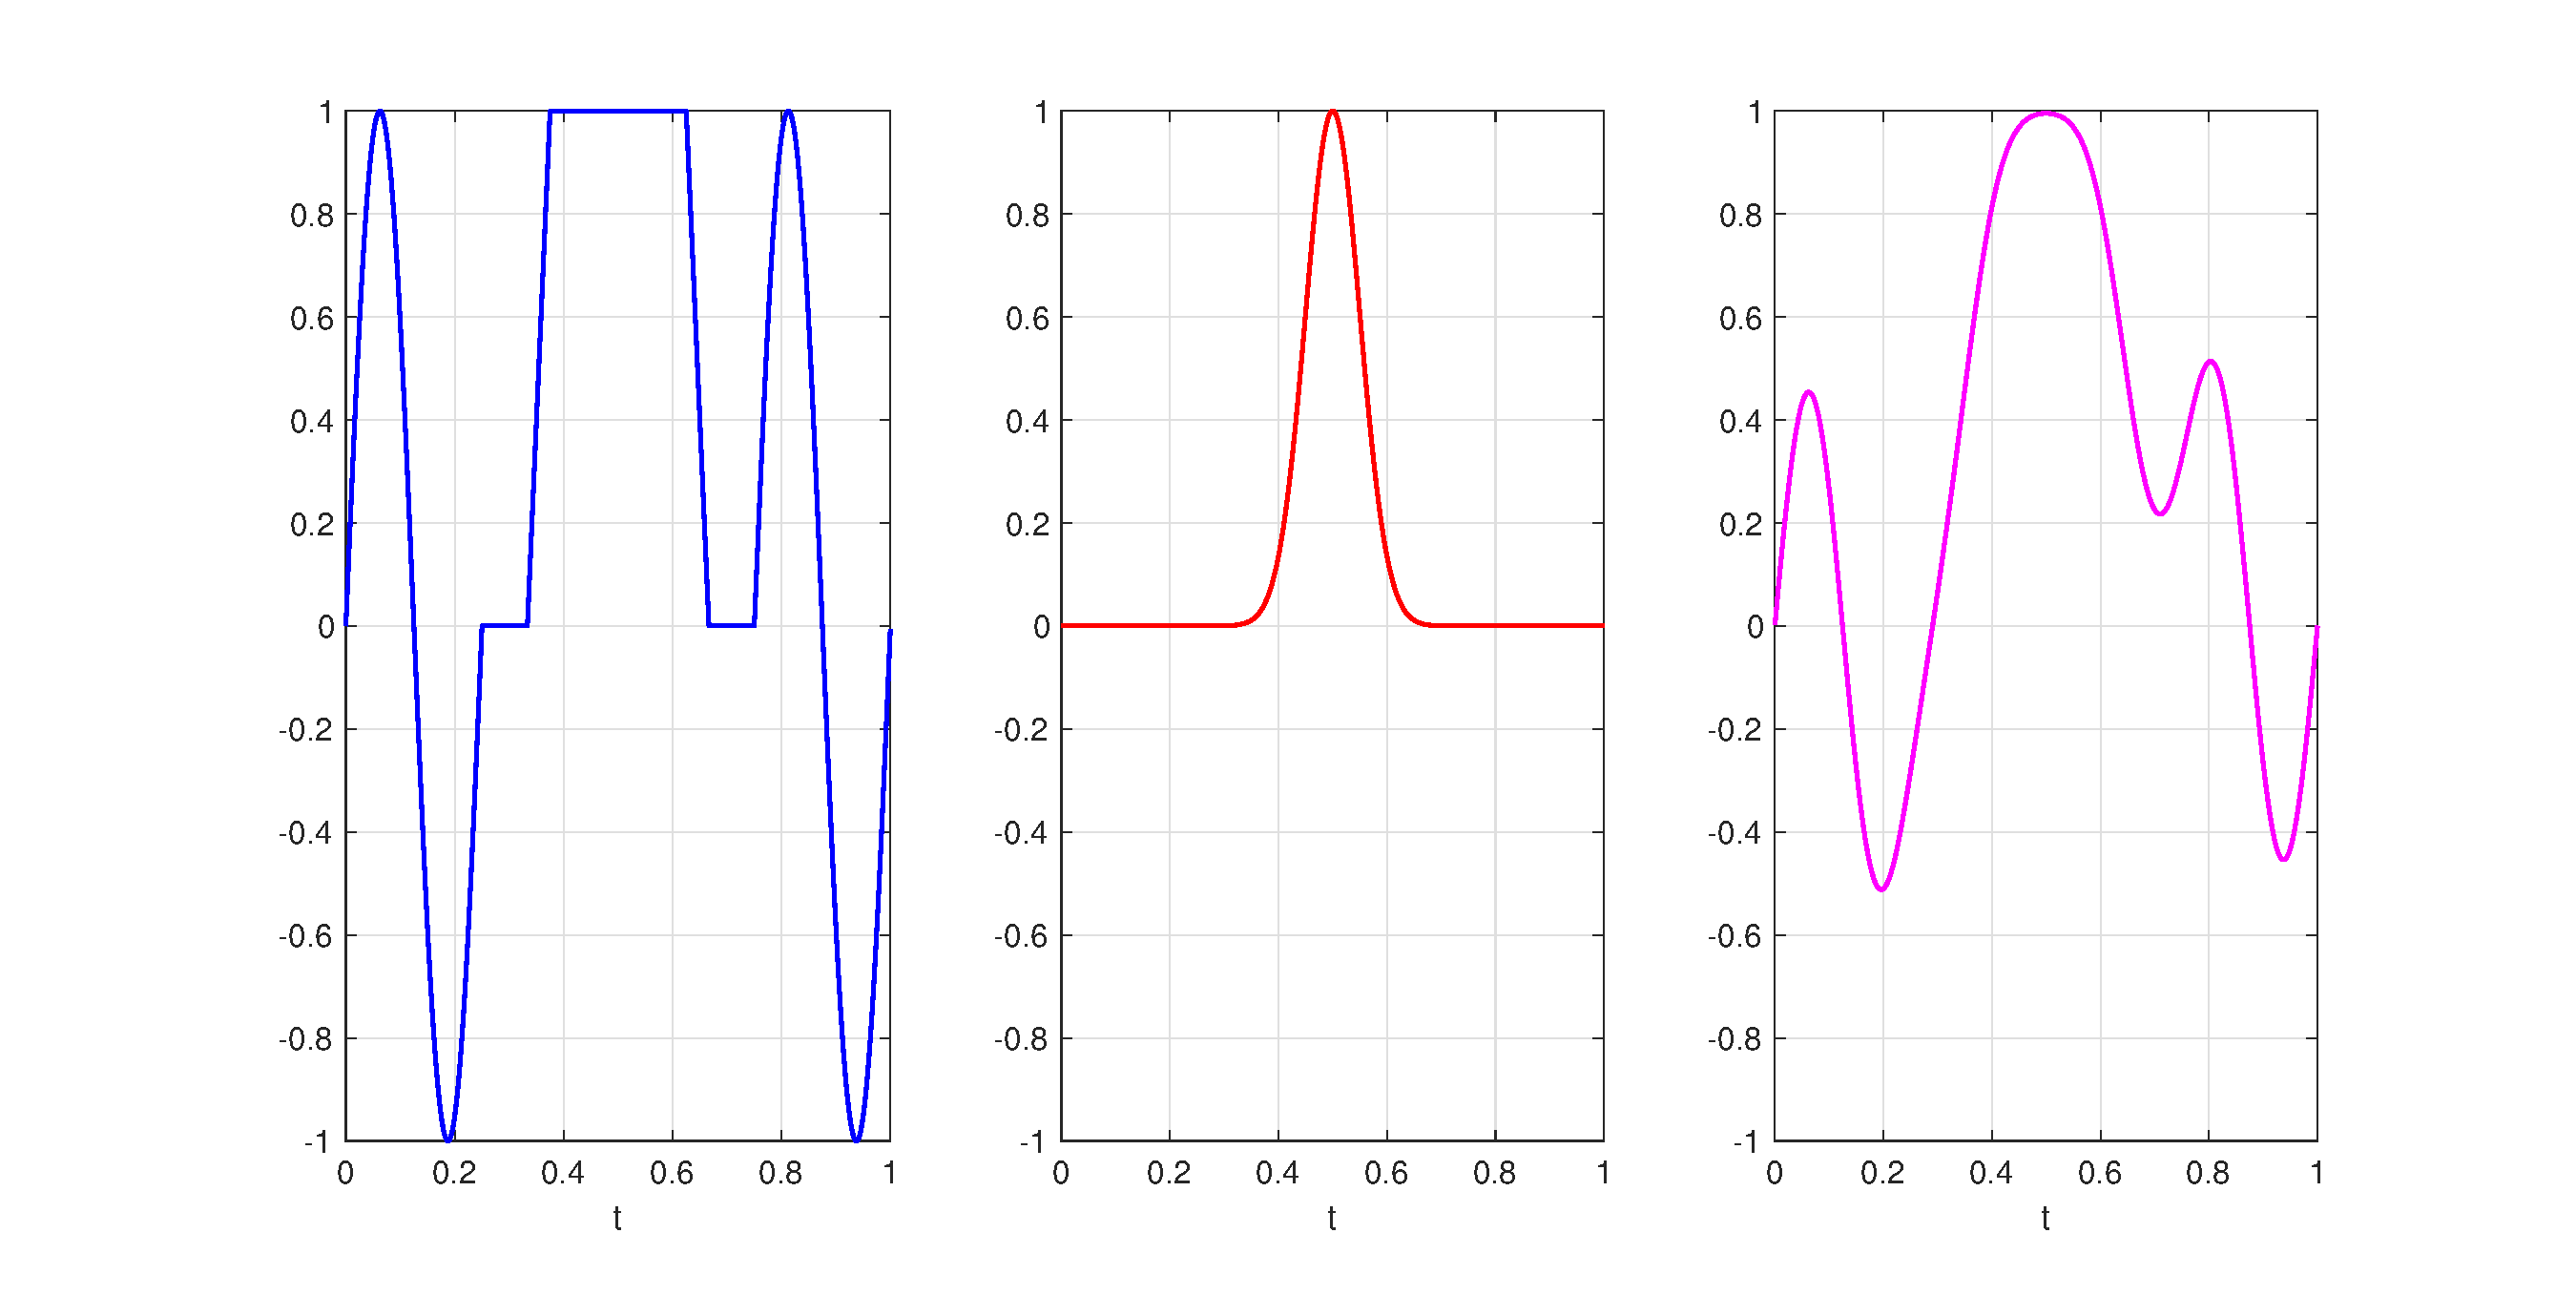
\includegraphics[scale=0.4]{Figures/FunctionKernelPlot.eps}}
\caption{Left: The graphs of the piecewise-smooth function $f(t)$ given by \eqref{eq:Test Function 2}. Center: The Gaussian kernel $k(t)$. Right: The function $g(x) = (f * g)(x)$. Notice that the corners of the graph of $f(t)$ have been smoothed over as a result of the convolution.}
\label{FunctionKernelPlot}
\end{figure}

\begin{figure}
	\centerline{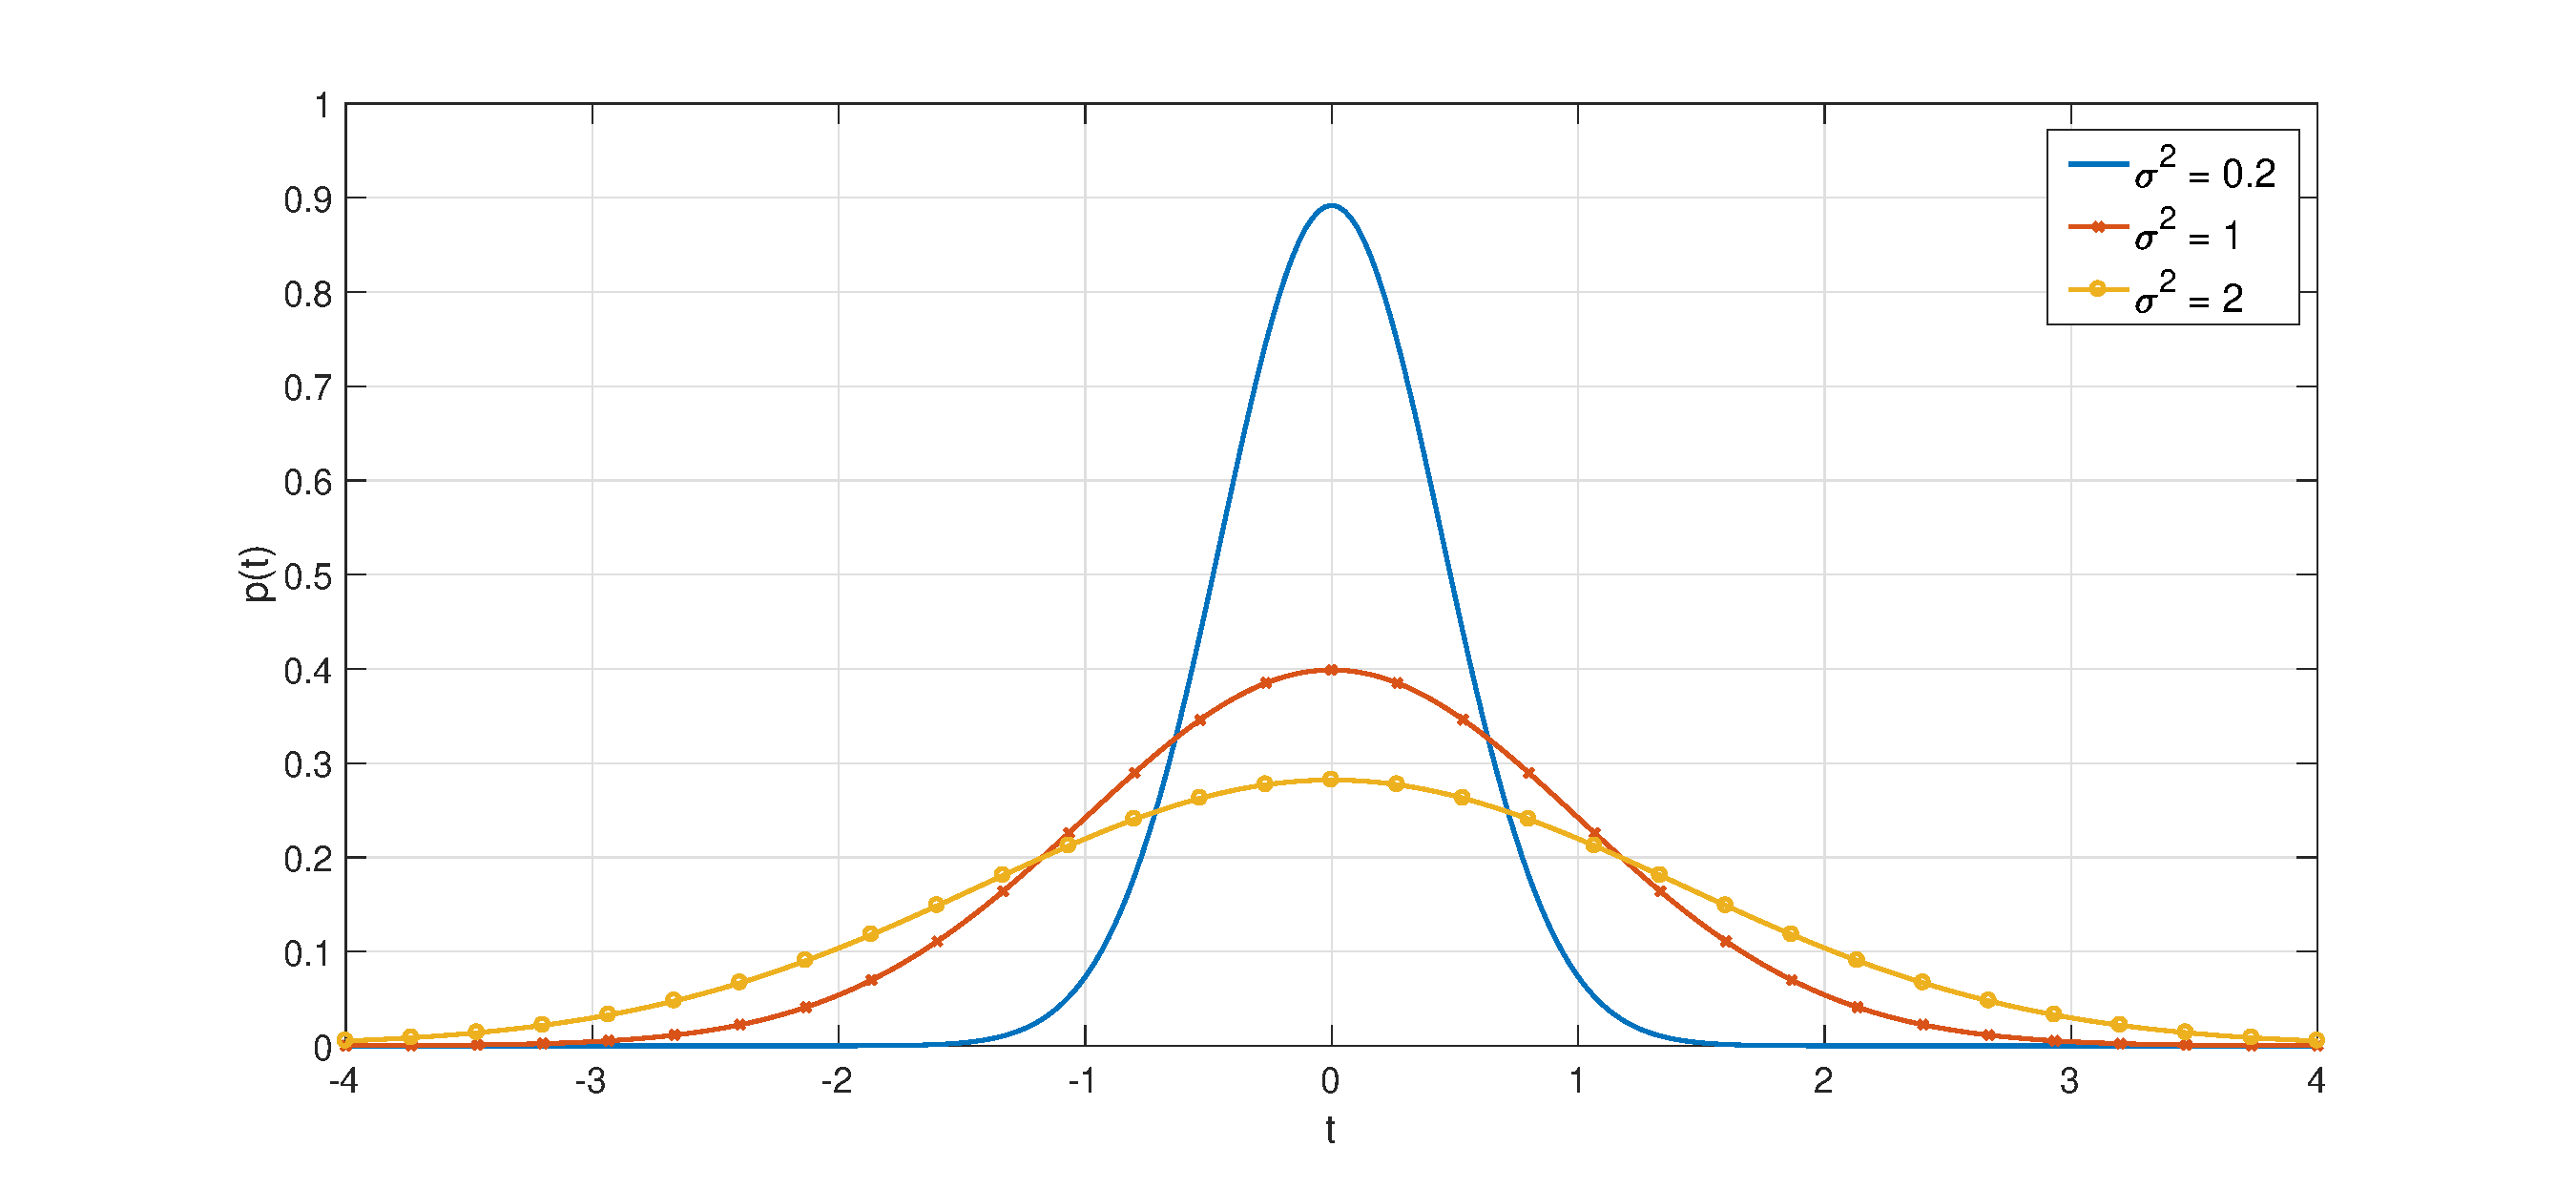
\includegraphics[scale=0.4]{Figures/GaussianDistributions.eps}}
\caption{Gaussian distributions for difference values of variance $\noiseSD^2$, all centered at the origin ($\mu = 0$). As $\noiseSD^2$ increases, the width of the distribution increases.}
\label{GaussianDistributions}
\end{figure}

If the kernel $k(x-t)$ in \eqref{eq:FIE} has compact support, then the limits of integration can be expressed as finite values that depend upon the support of $k(x-t)$. For example, if the support of $k(x-t)$ is $[\alpha_k,\beta_k]$, then \eqref{eq:FIE} becomes
\begin{equation}
\label{eq:FIE 2}
g(x) = \int_{-\infty}^{\infty} k(x-t)f(t) ~dt = \int_{x-\beta_k}^{x-\alpha_k} k(x-t)f(t) ~dt.
\end{equation} 
More rigorously, if $k(x-t)$ is compactly supported and $f(t)$ is locally integrable, then $g(x) = (k*f)(x)$ exists and is continuous. Existence follows directly from the condition of local integrability, which means that $\int_a^b f(t) ~dt$ exists for every $-\infty < a < b < \infty$; the space of locally integrable functions is a subspace of $L^1(\mathbb{R})$ \cite[p.~63]{DebnathMikusinski2005}. In real-world applications, data is finite and in the context of \eqref{eq:FIE}, this means that information about $g(x)$ is only known over a finite interval. Suppose information about $g(x)$ is only known over the interval $[\alpha_g,\beta_g]$. Then using \eqref{eq:FIE 2}, $g(\alpha_g)$ and $g(\beta_g)$ are given by
\[g(\alpha_g) = \int_{\alpha_g-\beta_k}^{\alpha_g-\alpha_k} k(\alpha_g - t)f(t) ~dt, \quad g(\beta_g) = \int_{\beta_g - \beta_k}^{\beta_g - \alpha_k} k(\beta_g-t)f(t) ~dt.\]
Without loss of generality, suppose $[\alpha_k,\beta_k] = [-\frac{1}{2},\frac{1}{2}]$ and $[\alpha_g,\beta_g] = [0,1]$. Then $\alpha_g-\beta_k = -\frac{1}{2}$ and $\beta_g - \alpha_k = \frac{3}{2}$, meaning that the support of $f(t)$ affecting the given data about $g(x)$ is $[-\frac{1}{2},\frac{3}{2}]$. In other words, if a solution $f(t)$ is only desired over the support of $g(x)$, then boundary conditions must be imposed on $f(t)$ so that the corresponding discrete system will not be underdetermined; this is addressed in Chapter \ref{ch:Results}. \par 
To find a solution to the forward problem, which is the evaluation of $g(x) = (k * f)(x)$, a quadrature method can be used to find a numerical approximation to the convolution integral. In the discrete setting, (1) can be stated as
\begin{equation}
\bVec = A\xVec,
\label{eq:Dis}
\end{equation}
where $\xVec$ and $\bVec$ are the vector discretization of $f(t)$ and $g(x)$, respectively, and $A$ is a matrix representing the discrete convolution of $k(x,t)$ with $f(t)$. For example, suppose $k(x,t)$ is a zero-centered Gaussian kernel and the domain of integration in \eqref{eq:FIE} is $[0,1]$. Given some $x_j \in [0,1]$, the continuous forward problem is to evaluate
\[g(x_j) = \int_0^1 \exp\left(\frac{-(x_j - t)^2}{2\noiseSD^2}\right)f(t) \: dt.\]
If a left Riemann sum is used with $t_k = k/n$ for $k \in \{0,1,\ldots,n-1\}$, representing an equispaced discretization of $[0,1]$ using $n$ points, then
\[g(x_j) \approx \sum_{k=1}^n \frac{1}{n}\exp\left(\frac{-(x_j - t_k)^2}{2\noiseSD^2}\right)f(t_j).\]
For approximations to $g(x)$ at the same points that make up the equispaced discretization of $[0,1]$, i.e. at the points $x_j = j/n$ for $j \in \{0,1,\ldots,n-1\}$, then \eqref{eq:Dis} is exactly the system that provides these approximations with $\xVec = [x(t_0),x(t_1),\ldots,x(t_{n-1})]$, $\bVec = [g(x_0),g(x_1),\ldots,g(x_{n-1})]$, and the elements of $A$ being
\[A_{j,k} = \frac{1}{n}\exp\left(\frac{-(j - k)^2}{2\noiseSD^2}\right), \quad 0 \leq j,k \leq n-1.\]
Note that taking the collocation and quadrature points as the same ensures that the matrix $A$ is square. Changing the number of collocation points, or the quadrature method, can change $A$ from square to rectangular; see Section \ref{sec:DFT}. \par
If the matrix $A$ is nonsingular, then the solution to the inverse problem \eqref{eq:Dis} is $\xVec = \inv{A}\dVec$. As with many linear systems, however, direct matrix inversion is discouraged and usually impractical since the matrix $A$ can become increasingly ill-conditioned as the size of the system grows \cite[p.~2]{Vogel:2002}. Unfortunately, large systems are often necessary to adequately approximate the continuous problem, and so other methods of solving for $\xVec$ must be considered. \par
Before discussing the consequences of ill-conditioning, the concept of a well-posed problem will be introduced, which is due to Hadamard \cite{Hadamard1904}. Given an operator $A : \mathcal{H}_1 \rightarrow \mathcal{H}_2$, where $\mathcal{H}_1$ and $\mathcal{H}_1$ are Hilbert spaces, the equation $Af = g$ is said to be well-posed if
\begin{enumerate}
\item[(i)] for each $g \in \mathcal{H}_2$ there exists a solution $f \in \mathcal{H}_1$ to $Af = g$,
\item[(ii)] the solution $f$ is unique, and
\item[(iii)] if $Af_* = g_*$ and $Af = g$, then $f \rightarrow f_*$ whenever $g \rightarrow g_*$.
\end{enumerate}
In order, these conditions require that a solution exists, is unique, and is stable under perturbations in $g$. If one of these conditions is not met, then $Af = g$ is said to be an ill-posed problem. The discrete problem $A\xVec = \bVec$ can be ill-posed under a number of circumstances: singularity of $A$ violates conditions (i) and (ii), and a poor condition number of nonsingular $A$ violates condition (iii). If the matrix $A$ is rectangular, then $A$ is singular and certainly (i) is violated.  \par 
A primary consequence of $A$ being ill-conditioned relates to the accuracy of the vector $\bVec$. If $\bVec$ contains errors, as is often the case in practical applications, the errors are amplified during the multiplication $\inv{A}\bVec$ since $A$ is ill-conditioned. As a result, the obtained solution $\xVec$ will suffer from a large amount error; $\xVec$ is thus sensitive to errors in $\bVec$. For this consideration, the following system will be the assumed model
\begin{equation}
\dVec = A\xVec + \noiseVec,
\label{eq:DisNoise}
\end{equation}
where $\noiseVec$ is a vector that represents any errors in $\bVec$ (this is equivalent to the statement $\dVec = \bVec + \noiseVec$). For further simplicity, assume that $\noiseVec \sim \mathcal{N}(\zeroVec,\noiseSD^2I)$, where $\zeroVec$ is the zero vector of length $n$ and $I$ is the $n \times n$ identity matrix. In other words, the error vector $\noiseVec$ is a realization of an $n$-dimension Gaussian random variable with mean zero and variance $\noiseSD^2$. 

\section{Main contributions and overview}
The contributions of this research are twofold. First, the regularization parameter estimation functions pertaining to the unbiased predictive risk estimator, the generalized cross validation method, and the discrepancy principle are formulated from the perspective of the discrete Fourier and cosine transform. In other words, the functions use the discrete Fourier and cosine transform components as opposed to singular values. Second, the effects of downsampling on parameter estimation are evaluated both qualitatively and quantitatively. The qualitative characteristics of these effects can be analyzed by using empirical statistics obtained from numerical examples in conjunction with multiple realizations of noise (see Section \ref{sec:Downsampling and white noise}). The quantitative characteristics are currently incomplete and are one of the goals of future research. \par
Chapter \ref{ch:Analytical tools} will present tools and ideas that are commonly used for the solution of inverse problems. Two primary tools, the discrete  Fourier and cosine transforms, are discussed in Section \ref{sec:Discrete trig. transforms}. The numerical examples considered in conjunction with these transforms are explained in Chapter \ref{ch:Results}. \par 
Since the assumed model problem \eqref{eq:DisNoise} contains random noise, a discussion of statistical results is included in Chapter \ref{ch:Stats}. The statistical results pertain not only to the nature of the noise under various transformations but also serve as a motivation for the parameter estimation methods contained in Chapter \ref{ch:Parameter estimation methods}. In addition to introducing the parameter estimation methods, Chapter \ref{ch:Parameter estimation methods} also presents new formulations of the parameter estimation functions which are based on the DFT and DCT. Versions of the the parameter estimation functions which assume the availability multiple data sets are available are also provided.  \par  
A two-dimension problem is considered in Chapter \ref{ch:Results}, which presents some of the interesting extensions of the one-dimensional concepts. Lastly, some conclusions and observations are made in Chapter \ref{ch:Conclusion}. The observations are used to motivate the goals of future work, which include consideration of three-dimensional numerical examples and quantitative descriptions of the effects of downsampling.

\chapter{Analytical tools} \label{ch:Analytical tools}

A number of analytic tools will be utilized. The singular value decomposition and the numerical difficulties of direct inversion are covered in Section \ref{sec:SVD}; these numerical difficulties will motivate the need for regularization. Section \ref{sec:Tikhonov reg.} introduces Tikhonov regularization, as well as a discussion regarding the forms in which Tikhonov regularization can be stated.  To conclude the chapter, Section \ref{sec:Classes of matrices} presents some of the properties of a number of classes of matrices that will be used in later chapters.

\section{The Singular Value Decomposition} \label{sec:SVD}

Direct matrix inversion is not always practical, and not even possible when $\kMat$ can be singular. Fortunately, the singular value decomposition (SVD) of $\kMat$ can used instead if the system is not too large. Even for problems resulting in large discrete systems, the SVD is useful for analyzing solution methods.  Assuming $\kMat$ is a real $m \times n$ matrix, the SVD of $\kMat$ is
\begin{equation}
\kMat = U\Sigma\trans{V}
\label{eq:SVD}
\end{equation}
where the $m \times m$ matrix $U$ and the $n \times n$ matrix $V$ have orthogonal columns and $\Sigma$ is a $m \times n$ diagonal matrix. The diagonal elements of $\Sigma$ are the singular values of $\kMat$, denoted $\singular_\ell$ and satisfying $\singular_0 \geq \singular_1 \geq \ldots \geq \singular_{n-1} \geq 0$. The columns of $U$ and $V$ will be denoted $U_{\cdot,\ell}$ and $V_{\cdot,\ell}$, respectively; these vectors are known as the left and right singular vectors of $\kMat$, respectively. A matrix of complex values has a SVD as well, the only difference being that the transpose is replaced with conjugate transpose. \par
Let $r$ denote the rank of $\kMat$. Then $\singular_0 \geq \ldots \geq \singular_{r-1} > 0$, i.e. the number of nonzero singular values of $\kMat$ is equal to the rank of $\kMat$.  A common variation of the SVD is the compact SVD (or economy SVD \cite{GolubVanLoan2013}), in which $\Sigma = \diag(\singular_0,\ldots,\singular_{r-1})$, $U$ is an $m \times r$ matrix and $\trans{V}$ is an $r \times n$ matrix. The matrices $U$ and $V$ are no longer orthogonal in the traditional sense because they are not square (unless $\kMat$ is nonsingular). Instead, $U$ and $V$ are column orthonormal. \par 
By using $\kMat^{-1} = V\Sigma^{-1}\trans{U}$ when $\kMat$ is nonsingular, the product $\kMat^{-1}\gnoiseVec$ is
\begin{equation}
\kMat^{-1}\gnoiseVec = \kMat^{-1}\left(\kMat\fVec + \noiseVec\right) = \fVec + \kMat^{-1}\noiseVec = \fVec + V\Sigma^{-1}\trans{U}\noiseVec = \fVec + \sum_{\ell = 0}^{n-1} \frac{\trans{U}_\ell\noiseVec}{\singular_\ell}V_{\cdot,\ell}. 
\label{eq:InvProd}
\end{equation}
Even if $\kMat$ is singular, a solution can still be obtained by using the pseudoinverse $\kMat^\dagger = V{\Sigma^\dagger}\trans{U}$, where $\Sigma^\dagger = \diag(1/\singular_0,\ldots,1/\singular_{r-1})$, and the upper bound of summation in \eqref{eq:InvProd} becomes $r-1$. In either the nonsingular or singular case for $\kMat$, however, the summands in \eqref{eq:InvProd} are numerically unstable for small $\singular_\ell$. For a visual representation of this instability, a Picard plot can be constructed. A Picard plot is a graph showing the terms $|\trans{U}_{\cdot,\ell}\noiseVec|/\singular_\ell$ in decreasing order with respect to the singular values. If the terms $|\trans{U}_{\cdot,\ell}\noiseVec|$ decay faster than $\singular_\ell$ as $\ell$ increases, then the terms $|\trans{U}_{\cdot,\ell}\noiseVec|/\singular_\ell$ do not become excessively large; this is the discrete Picard condition \cite{ABT}. The discrete Picard condition is thus a measure of instability. If the discrete Picard condition is not met, then the terms $|\trans{U}_{\cdot,\ell}\noiseVec|/\singular_\ell$ blow up as $\ell$ increases, often resulting in worthless solutions. In this report, the discrete Fourier and cosine transforms will be used to obtain solutions analogous to those obtained by \eqref{eq:InvProd}. Figure \ref{PicardPlot} in Chapter \ref{ch:DFT} is an example of a Picard plot is provided that demonstrates the relationship between the noise, the width of the Gaussian blur, and the resulting numerical instabilities related to obtaining meaningful solutions. See \cite{Hansen1990} for more information on Picard plots and the associated discrete Picard condition. \par 
A common approach to overcome numerical instabilities is to multiply the summands in \eqref{eq:InvProd} by \textit{filter functions} $\filt$ that depend upon $\singular_\ell$ and a non-negative \textit{regularization parameter} $\regparam$. By doing so, an approximate solution is obtained:
\begin{equation}
\fVec_\regparam = \sum_{\ell = 0}^{n-1} V_{\cdot,\ell}\filt(\regparam,\singular_\ell)\left(\frac{{\trans{U}_\ell}\gnoiseVec}{\singular_\ell}\right) = V\Phi\Sigma^\dagger \trans{U}\gnoiseVec,
\label{eq:ApproxSol}
\end{equation}
where the matrix $\Phi$ is diagonal with $\Phi_{\ell,\ell} = \filt(\regparam,\singular_\ell)$ for $\ell = 0,\ldots,{n-1}$. The most desired property of the filter functions is that $\filt(\singular_\ell)/\singular_\ell \approx 1$  for large values of $\singular_\ell$ and $\filt(\singular_\ell)/\singular_\ell \approx 0$ for small values of $\singular_\ell$.  Perhaps the simplest filter function is
\[\filt(\regparam,\singular_\ell) = \begin{cases}
1, & \singular_\ell^2 > \regparam \\
0, & \singular_\ell^2 \leq \regparam
\end{cases}\]
Using this function in (3) gives the approximate solution
\[\fVec_\regparam = \sum_{\singular_\ell^2 > \regparam} \frac{{\trans{U}_\ell}\gnoiseVec}{\singular_\ell}V_{\cdot,\ell}\]
which actually corresponds to the solution obtained using a truncated singular value decomposition (TSVD) of the matrix $\kMat$ \cite[p.~3-5]{Vogel:2002}. \par

\section{Tikhonov regularization} \label{sec:Tikhonov reg.}

A less simple filter function is
\begin{equation}
\filt(\regparam,\singular_\ell)  = \frac{\singular_\ell^2}{\singular_\ell^2 + \regparam^2}
\label{eq:TikFilt}
\end{equation}
which is known as the Tikhonov filter function. For large values of $\regparam$, \eqref{eq:TikFilt} is close to zero and for small values of $\regparam$ (and nonzero values of $\singular_\ell$), it is close to one. Another property of \eqref{eq:TikFilt} is that for fixed nonzero $\singular_\ell$, it is monotone decreasing in $\regparam$. Since the expression $1 - \filt(\regparam,\singular_\ell)$ arises a number of times in the methods introduced in Chapter \ref{ch:Parameter estimation methods}, let
\begin{equation}
\mfilt(\regparam,\singular_\ell) = 1 - \filt(\regparam,\singular_\ell) = \frac{\regparam^2}{\singular_\ell^2 + \regparam^2}.
\label{eq:TikFiltPsi}
\end{equation}
to simplify notation. In contrast to \eqref{eq:TikFilt}, \eqref{eq:TikFiltPsi} is close to one for large values of $\regparam$ and monotone increasing in $\regparam$ for fixed $\singular_\ell$; see Figure \ref{fig:Phi Psi Plot}. \par 

\begin{figure}
	\centerline{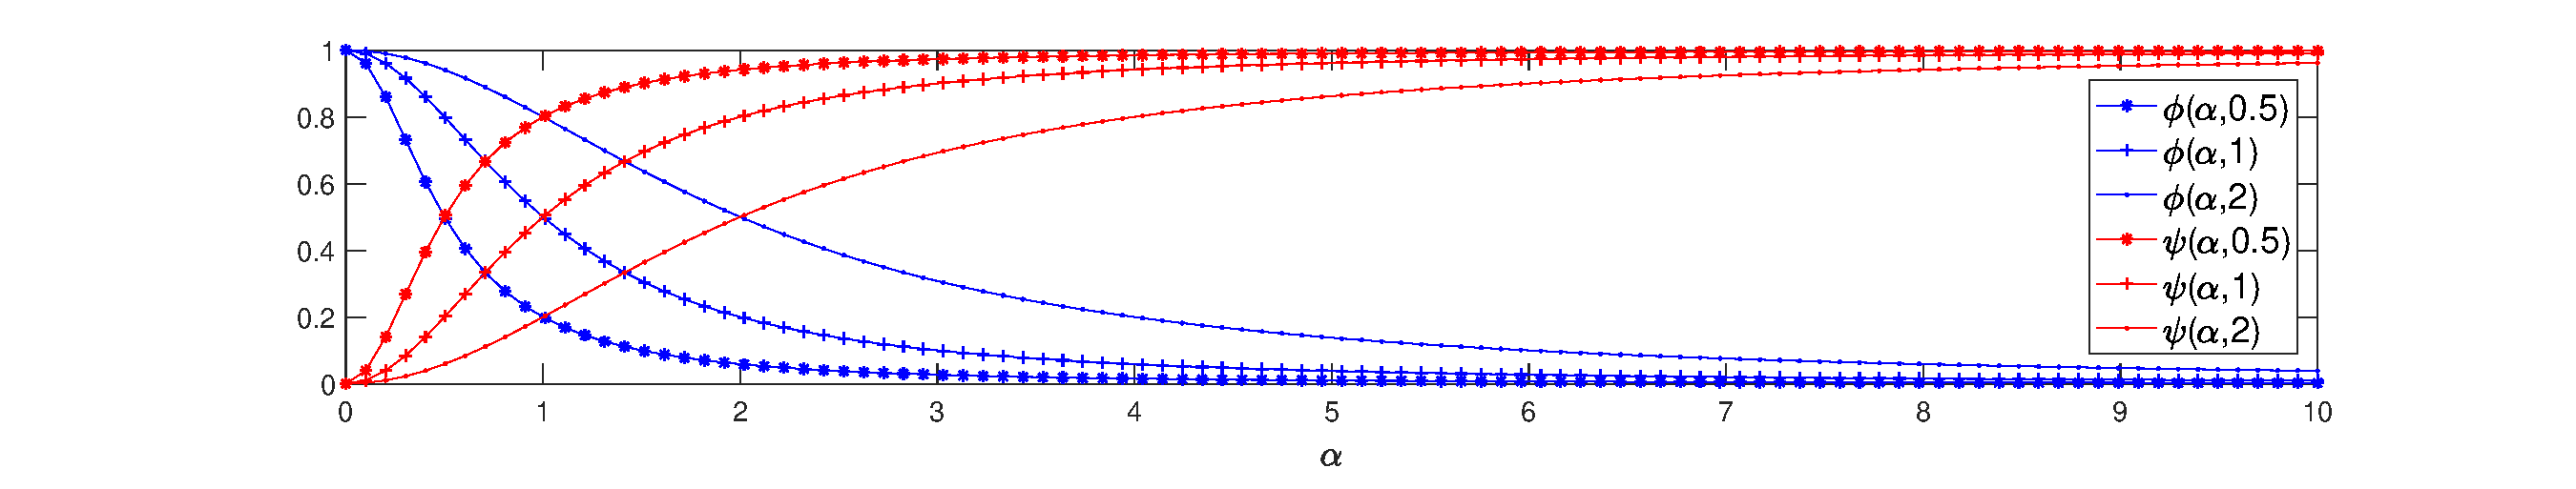
\includegraphics[scale = 0.4]{Figures/Phi_Psi_Plot.eps}}
\caption{The behavior of the Tikhonov filter function $\filt(\regparam,\singular_\ell)$ and corresponding $\mfilt(\regparam,\singular_\ell) = 1 - \filt(\regparam,\singular_\ell)$ is displayed for choice values of $\singular_\ell$. For fixed $\singular_\ell$, $\filt(\regparam,\singular_\ell) \rightarrow 0$ and $\mfilt(\regparam,\singular_\ell) \rightarrow 1$ as $\regparam \rightarrow \infty$. Notice also that $\filt(\regparam,\singular_\ell) = \mfilt(\regparam,\singular_\ell) = 1/2$ for $\alpha = \singular_\ell$.}
\label{fig:Phi Psi Plot}
\end{figure}

The use of the Tikhonov filter function to generate an approximate solution is known as \textit{Tikhonov regularization} \cite{Tikh1963}; in terms of an SVD, the obtained solution is
\begin{equation}
\fVec_\regparam = \sum_{\ell = 1}^n \filt(\regparam,\singular_\ell)\frac{{\trans{U}_\ell}\gnoiseVec}{\singular_\ell}V_{\cdot,\ell} = \sum_{\ell = 0}^{n-1} \frac{\singular_\ell{\trans{U}_\ell}\gnoiseVec}{\singular_\ell^2 + \regparam^2}V_{\cdot,\ell} = V\Phi\Sigma^\dagger \trans{U}\gnoiseVec.
\label{eq:TikSol}
\end{equation}
An alternative (and more general) representation of the above Tikhonov solution is
\begin{equation}
\fVec_\regparam = \argmin_{\fVec \in \mathbb{R}^n} \left\{\|\kMat\fVec - \gnoiseVec\|^2 + \regparam^2\|D\fVec\|^2\right\},
\label{eq:TikSol2}
\end{equation}
where $D$ is the matrix representation of a linear operator and $\|\cdot\|$ is the 2-norm. The term $\|D\fVec\|^2$ is commonly called the penalty function \cite{Vogel:2002}. The representation \eqref{eq:TikSol} follows from selecting $D$ to be $I$, the $n \times n$ identity matrix. The solution \eqref{eq:TikSol2} can also be expressed in block form as
\begin{equation}
\fVec_\regparam = \argmin_{\fVec \in \mathbb{R}^n} \left\| \begin{bmatrix}
\kMat \\
\regparam D
\end{bmatrix}\fVec - \begin{bmatrix}
\gnoiseVec \\
\zeroVec
\end{bmatrix} \right\|^2.
\label{eq:TikSol3}
\end{equation}
If the matrix $D$ in \eqref{eq:TikSol2} is non-singular, then the substitutions $\mathbf{y} = D\fVec$, $A = \kMat{D}^{-1}$, and $\mathbf{b} = \gnoiseVec$ give
\begin{equation}
\mathbf{y}(\regparam) = \argmin_{\mathbf{y} \in \mathbb{R}^n} \|A\mathbf{y} - \mathbf{b}\|^2 + \regparam^2\|\mathbf{y}\|^2.
\label{eq:TikSol Standard Form}
\end{equation}
This is known as standard form of the regularization problem. Once $\mathbf{y}$ is obtained from \eqref{eq:TikSol Standard Form}, the final solution is recovered by $\fVec = D^{-1}\mathbf{y}$.  \par 
However, there are many examples of matrices $D$ that are singular, such as finite difference matrices that approximate derivative operators. In such cases, the regularization can still be recast in standard form, which can be accomplished in a convenient way using the generalized singular value decomposition (GSVD). To simplify the derivation of the GSVD, it will be assumed that the matrix $\trans{[\kMat, \regparam D]}$ in \eqref{eq:TikSol3} has full column rank, i.e. $\nullspace(\kMat) \cap \nullspace(D) = \varnothing$, which ensures that the solution $\fVec_\regparam$ is unique. Another simplifying assumption being that the $p \times n$ matrix $D$ with $p \leq n$ has full row rank. Under these assumptions \cite[p.~104]{ABT}, the matrices $\kMat$ and $D$ can be expressed as
\begin{equation}
\label{eq:GSVD matrices}
\kMat = U\Lambda \trans{X}, \quad D = VM\trans{X}
\end{equation}
where the matrices $U$, $V$, $\Lambda$, $M$, and $X$ satisfy the following: 
\begin{itemize}
\item $U$ is an orthogonal $m \times m$ matrix. 
\item $V$ is an orthogonal $p \times p$ matrix.
\item $\Lambda$ is an $m \times n$ matrix with the property that the nonzero entries satisfy
\[0 \leq \Lambda_{1,k+1} \leq \ldots \leq \Lambda_{m,k+m} \leq 1,\]
where $k = 0$ if $m > n$ and $k = n-m$ otherwise. 
\item $M$ is a diagonal $p \times n$ matrix with $M_{1,1} \geq \ldots \geq M_{p,p} \geq 0.$
\item $\trans{M} M + \trans{\Lambda} \Lambda = I$ (the dimension of the identity matrix being $n \times n$).
\item $X$ is a nonsingular $n \times n$ matrix.
\end{itemize}
The generalized singular values of $\kMat$ and $D$ are defined as $\gamma_\ell = \lambda_{\ell}/\mu_{\ell}$, where
\begin{equation}
\label{eq:GSVD lambda}
\lambda_\ell = \sqrt{(\trans{\Lambda} \Lambda)_{\ell,\ell}}, \quad \mu_\ell = \sqrt{(\trans{M} M)_{\ell,\ell}}
\end{equation}
for $\ell = 0,\ldots,{n-1}$. In contrast to the SVD, the generalized singular values are ordered $\gamma_0 \leq \ldots \leq \gamma_{n-1}$. It is also possible that $\mu_\ell = 0$ for some $\ell$, in which case $\gamma_\ell$ is not defined. Even when $\mu_\ell$ is small the resulting value of $\gamma_\ell$ can be excessively large, again emphasizing the need for regularization. By applying the orthogonality properties of the GSVD matrices \cite[p.~105-106]{ABT}, the regularized solution \eqref{eq:TikSol3} can be expressed as
\begin{equation}
\label{eq:TikSol GSVD}
\fVec_\regparam = \sum_{\ell=0}^{n-1} \frac{\gamma_\ell^2}{\gamma_\ell^2 + \regparam^2} \frac{\trans{U}_{\cdot,\ell+k}\gnoiseVec}{\lambda_\ell}Y_{\cdot,\ell}
\end{equation}
where $Y = \invTrans{X}$ (the inverse of $\trans{X}$). The terms $\gamma_\ell^2/(\gamma_\ell^2 + \regparam^2)$ are known as the GSVD filter factors, which are identical in form to the filter factors \eqref{eq:TikFilt}. \par 
With the derivation of the GSVD established, an extension of the transformation that rendered \eqref{eq:TikSol Standard Form} is now stated \cite[p.~38]{Hansen:98}. First, a weighted version of the pseudoinverse $D^\dagger$ is defined as
\[D_{\kMat}^\dagger = \left(I - \left(\kMat\left(I - D^\dagger D\right)\right)^\dagger \kMat\right)D^\dagger.\]
If $p \geq n$, then $D_{\kMat}^\dagger$ is the same as $D^\dagger$. We must also consider
\[\fVec_0 \equiv \left(\kMat\left(I - D^\dagger D\right)\right)^\dagger \gnoiseVec,\]
which is the component of the solution contained in $\nullspace(D)$.  Using the GSVD matrices from \eqref{eq:GSVD matrices}, $D_{\kMat}^\dagger$ and $\fVec_0$ can be written as
\begin{equation}
\label{eq:Trans. 1}
D_{\kMat}^\dagger = X \begin{bmatrix}
M^{-1} \\
\mathbf{0}
\end{bmatrix}\trans{V}, \quad \fVec_0 = \sum_{\ell=m+1}^{n} \trans{U}_{\cdot,\ell}\gnoiseVec X_{\cdot,\ell}
\end{equation}
where $\zeroVec$ is the zero matrix of appropriate dimension. The form of the regularized solution can be expressed as \eqref{eq:TikSol Standard Form} with substitutions $\mathbf{y} = D\fVec$, $A = \kMat{D_{\kMat}^\dagger}$, and $\mathbf{b} = \gnoiseVec - \kMat\fVec_0$. 
%This is shown by writing
%\begin{align*}
%\|A\mathbf{y} - \mathbf{b}\|^2 + \regparam^2\|\mathbf{y}\|^2 &= \|\kMat{D_{\kMat}^\dagger}D\fVec - (\gnoiseVec - \kMat\fVec_0)\|^2 + \regparam^2\|D\fVec\|^2 \\
%&=  \|\kMat({D_{\kMat}^\dagger}D\fVec + \fVec_0) - \gnoiseVec\|^2 + \regparam^2\|D\fVec\|^2
%\end{align*}
%as well as 
%\ToDo{
%\begin{align*}
%{D_{\kMat}^\dagger}D\fVec + \fVec_0 &= \left(I - \left(\kMat\left(I - D^\dagger D\right)\right)^\dagger \kMat\right)D^\dagger D\fVec + \left(\kMat\left(I - D^\dagger D\right)\right)^\dagger \gnoiseVec \\
%&= D^\dagger D\fVec - \left(\kMat\left(I - D^\dagger D\right)\right)^\dagger \kMat D^\dagger D\fVec + \left(\kMat\left(I - D^\dagger D\right)\right)^\dagger \gnoiseVec \\ 
%&= D^\dagger D\fVec + \left(\kMat\left(I - D^\dagger D\right)\right)^\dagger \left[\gnoiseVec - \kMat D^\dagger D\fVec\right] \\
%&= 
%\end{align*}}
The final solution is then recovered by $\fVec = D_{\kMat}^\dagger \mathbf{y} + \fVec_0$. 

%\section{Discrete convolution} \label{sec:Discrete convolution}
%As described in the Chapter \ref{ch:Introduction}, the operation of convolution arises in various settings pertaining to inverse problems. Discrete convolution will first be described  in a general setting, followed by specific instances and connections to appropriate numerical examples. \par
%Let $(x_n)$ and $(y_n)$ be sequences of complex numbers indexed by the integers. Then the discrete convolution of $(x_n)$ and $(y_n)$, denoted $x*y$, is defined by
%\[(x*y)_n = \sum_{\ell=-\infty}^\infty x_{n-\ell}y_\ell.\]
%The series in the definition of discrete convolution is bi-infinite, meaning that the discrete convolution might not be well-defined for any two arbitrary sequences. For example, if $x_n = y_n = 1$ for all $n \in \mathbb{Z}$, then the series defining $(x*y)_n$ is $\sum_{j=-\infty}^\infty 1$, which does not converge. In various cases, however, the discrete convolution is well-defined. These cases include sequences having only finitely-many nonzero terms and sequences in $\ell^1$. (In fact, the set of sequences having finitely-many nonzero terms is a linear subspace of $\ell^1$).  \par 
%Fortunately, real-world applications usually involve finite sequences (vectors), which can be thought of as infinite or bi-infinite sequences having finitely-many nonzero terms. While such sequences do not require the evaluation of infinite series to compute discrete convolutions, it is helpful to have general results regarding the length and indices of discrete convolutions. Let $(x_n)$ and $(y_n)$ be nonzero sequences with finitely-many nonzero terms. For $(x_n)$, the assumptions imply the existence of integers $b_x$ and $e_x$ such that $x_n = 0$ for all $n \in \mathbb{Z}$ with either $n < b_x$ or $e_x < n$. Such integers exist for $(y_n)$ and will be denoted $b_y$ and $e_y$. The choice of letters reflects the fact that $s$ and $e$ represent the starting and ending indices of the section of the sequence where the terms can be nonzero. Extending this notation, the number of terms in this section of sequence is $n_x = e_x - b_x + 1$ and $n_y = e_y - b_y + 1$ for $(x_n)$ and $(y_n)$, respectively. From \cite{BoggessNarcowich2009}, the values of $s_{x*y}$, $e_{x*y}$, and $n_{x*y}$ are
%\begin{align}
%s_{x*y} &= b_x + b_y, \nonumber \\
%e_{x*y} &= e_x + e_y, \label{eq:FIEResults} \\
%n_{x*y} &= n_x + n_y - 1. \nonumber
%\end{align}
%As an illustrative example, let $\mathbf{x} = [1,2,3]$ and $\mathbf{y} = [4,5,6,7]$ be row vectors. The vectors can be thought of as the bi-infinite sequences $(x_n) = (\ldots,0,1,2,3,0\ldots)$ and $(y_n) = (\ldots,0,4,5,6,7,0,\ldots)$. If the sequences are indexed so that $x_1 = 1$ and $y_1 = 4$, then $b_x = b_y = 1$, $e_x = n_x = 3$, and $e_y = n_y = 4$. Then by \eqref{eq:FIEResults}, $s_{x*y} = 2$, $e_{x*y} = 8$, and $n_{x*y} = 6$. The bi-infinite sequence produced from the convolution is
%\[x*y = (\ldots,0,4,13,28,34,32,21,0,\ldots),\]
%where $(x*y)_2 = 4$ and $(x*y)_8 = 21$. \par 
%Since the numerical examples are conducted in MATLAB, a brief remark regarding discrete convolutions in MATLAB is be given. If the built-in function \texttt{conv} is used to evaluate the discrete convolution of row vectors $\mathbf{x}$ and $\mathbf{y}$ described in the previous example, the output is the row vector $[4,13,28,34,32,21]$.  All vectors in MATLAB have a starting index of 1, and the vector resulting from the convolution is no different: the component 4 has an index of 1. While this seems to conflict with \eqref{eq:FIEResults} (recall that $s_{x*y} = 2$, not 1), from a practical standpoint there is little reason for concern; usually the components themselves are of interest and not the indexing of the bi-infinite sequence. If one wants to keep track of the indexing as the convolution is evaluated, index vectors can be defined for $\mathbf{x}$ and $\mathbf{y}$ and \eqref{eq:FIEResults} can be applied to obtain an index vector for the resulting convolution. See \cite{BoggessNarcowich2009} for an explicit MATLAB example. \par 

\section{Classes of matrices} \label{sec:Classes of matrices}
The first type of matrix to be discussed is a \textit{Toeplitz matrix}. A matrix $T$ is called a Toeplitz matrix if it is constant along each diagonal. The following are examples of Toeplitz matrices:
\[A = \begin{bmatrix}
1 & 2 \\
3 & 1 \\
0 & 3
\end{bmatrix}, \quad 
B = \begin{bmatrix}
4 & 8 & 5 \\
7 & 4 & 8 \\
1 & 7 & 4
\end{bmatrix}.\]
By definition, Toeplitz matrices need not be square. However if a Toeplitz matrix is square with dimension $n \times n$, then it is uniquely determined by $2n-1$ entries. If a Toeplitz matrix is symmetric, then it is determined by $n$ entries. \par
Some notation for symmetric Toeplitz matrices will be introduced that will be used in Chapter \ref{ch:DCT}. Given a column vector $\mathbf{v}$ of length $n$, let $T(\mathbf{v})$ denote the $n \times n$ symmetric Toeplitz matrix with $\mathbf{v}$ as its first column. As example, the matrix $T(\mathbf{v})$ where $\mathbf{v} = \trans{[1,2,3,4]}$ is
\[T(\mathbf{v}) = \begin{bmatrix}
1 & 2 & 3 & 4 \\
2 & 1 & 2 & 3 \\
3 & 2 & 1 & 2 \\
4 & 3 & 2 & 1 
\end{bmatrix}.\] 
The primary connection to be made is that discrete convolutions can be described in the context of matrix-vector multiplication using Toeplitz matrices. For example, the discrete convolution of $\mathbf{x} = [1,2,3]$ and $\mathbf{y} = [4,5,6]$ can be cast as a matrix-vector product by defining a matrix $X$ to be
\[X = \begin{bmatrix}
1 & 0 & 0  \\
2 & 1 & 0 \\
3 & 2 & 1 \\
0 & 3 & 2 \\
0 & 0 & 3 
\end{bmatrix}.\]
Certainly $X$ is a Toeplitz matrix, and $x*y$ can be expressed as $X\trans{y}$ with $x*y$ being a (column) vector of length $n_{x*y} = 6$. The operation $X\trans{y}$ is equivalent to \texttt{conv(x,y)} in MATLAB. \par 
A type of matrix that is closely related to Toeplitz matrices is a Hankel matrix. A Hankel matrix is a matrix that is constant along each anti-diagonal. The following are examples of Hankel matrices:
\[A = \begin{bmatrix}
-1 & 2 \\
2 & 0 \\
0 & -6
\end{bmatrix}, \quad 
B = \begin{bmatrix}
1 & 2 & 5 \\
2 & 5 & 3 \\
5 & 3 & 9
\end{bmatrix}.\]
Similar to square Toeplitz matrices, a square Hankel matrix with dimension $n \times n$ is uniquely defined by $2n -1$ entries and symmetric Hankel matrices are determined by $n$ entries. Extending the notation for symmetric Toeplitz matrices, let $H(\mathbf{v})$ be the $n \times n$ symmetric Hankel matrix with the $n$-vector $\mathbf{v}$ as its first column. \par
A specific type of square Hankel matrix is the exchange matrix $J$, defined by ones along the main anti-diagonal and zero elsewhere. As a visual, the $4 \times 4$ exchange matrix is
\[J = \begin{bmatrix}
0 & 0 & 0 & 1 \\
0 & 0 & 1 & 0 \\
0 & 1 & 0 & 0 \\
1 & 0  & 0 & 0
\end{bmatrix}.\]
The exchange matrix is so-named for the property that the product of $J$ with a vector $\mathbf{v}$ has the effect of ``exchanging" (or ``reversing") the entries of $\mathbf{v}$. For example, if $\mathbf{v} = \trans{[1,2,3,4]}$ then $J\mathbf{v} = \trans{[4,3,2,1]}$. As a result of this property, the exchange matrix is an involution, i.e. $J^2 = I$. Another result of the properties of $J$ is that the product of a Toeplitz matrix with the exchange matrix is a Hankel matrix. Lemma \ref{lem:TJ = H} outlines a specific case where the Toeplitz matrix is symmetric.
\begin{lemma}
\label{lem:TJ = H}
Let $\mathbf{v} \in \mathbb{R}^n$ and let $J$ be the $n \times n$ exchange matrix. Then $T(J\mathbf{v})J = H(\mathbf{v})$.
\end{lemma}
\begin{proof}
By the symmetry of $T(J\mathbf{v})J$, it suffices to argue that the first column of $T(J\mathbf{v})J$ is $\mathbf{v}$. Since $T(J\mathbf{v})$ is post-multiplied by $J$, the first column of the product is equal to the last column of $T(J\mathbf{v})$. By definition, the last column of $T(J\mathbf{v})$ is $J(J\mathbf{v}) = J^2\mathbf{v} = \mathbf{v}$.
\end{proof}
If a matrix $C$ has the property that each row is the circular right shift of the components of the preceding row, then $C$ is called a \textit{circulant matrix}. The \textit{circular right shift} of a row vector $[x_0,x_1,\ldots,x_{n-1}]$ is $[x_{n-1},x_0,\ldots,x_{n-2}]$. From this definition, every circulant matrix is also a Toeplitz matrix. For example,
\[C = \begin{bmatrix}
1 & 2 & 3 & 4 \\
4 & 1 & 2 & 3 \\
3 & 4 & 1 & 2 \\
\end{bmatrix}\] 
is a circulant matrix generated by circular right shifts of the vector $[1,2,3,4]$. A final observation regarding circulant matrices can be made about their indexing. If $\mathbf{c} = [c_0,\cdots,c_{n-1}]$ is the first row of a circulant matrix $C$, then
\begin{equation}
\label{eq:Circulant indexing}
C_{j,k} = c_{k-j \bmod n}
\end{equation}
for all $0 \leq j,k \leq n-1$. A significant property of square circulant matrices discussed in Chapter \ref{ch:DFT} is that they are diagonalized by the discrete Fourier transform; \eqref{eq:Circulant indexing} can be used to prove this property.

\section{Discrete trigonometric transforms} \label{sec:Discrete trig. transforms}

The discrete Fourier transform will be introduced from the perspective of approximating coefficients of the Fourier series of a $2\pi$-periodic function $f$ \cite[p.~132-134]{BoggessNarcowich2009}. On the interval $[0,2\pi]$, the $j$th complex Fourier coefficient of $f(t)$ is given by
\[c_j = \frac{1}{2\pi}\int_0^{2\pi} f(t)\exp(-ijt)\:dt,\]
where $i = \sqrt{-1}$.  Applying the trapezoidal rule for approximating this integral with $n$ points then produces
\[c_j \approx \frac{1}{n}\sum_{\ell = 0}^{n-1} f\left(\frac{2\pi{\ell}}{n}\right)\exp\left(\frac{-2\pi{ij\ell}}{n}\right).\]
The \textit{discrete Fourier transform} (DFT) is a mapping $\mathcal{F}:\mathbb{C}^n \rightarrow \mathbb{C}^n$ defined by
\begin{equation}
\mathcal{F}(\mathbf{f})_j = \frac{1}{\sqrt{n}}\sum_{\ell=0}^{n-1} f_{\ell}\exp\left(\frac{-2\pi{ij\ell}}{n}\right), \quad \mathbf{f}\in\mathbb{C}^n, \quad 0 \leq k \leq n-1.
\label{eq:DFT}
\end{equation}
The DFT of a vector $\mathbf{f}$ will be denoted by $\dft{\mathbf{f}}$. The inverse DFT of a vector $\dft{\mathbf{f}}$ is given by
\begin{equation}
\mathcal{F}^{-1}(\dft{\mathbf{f}})_j = \frac{1}{\sqrt{n}}\sum_{\ell=0}^{n-1} \dft{f}_\ell\exp\left(\frac{2\pi{ij\ell}}{n}\right) = f_j.
\end{equation}
These definitions are nonstandard; typically the factors $1/\sqrt{n}$ in both the forward and inverse DFT definitions are combined as a single factor of $1/n$ in the definition of the forward DFT. The DFT can also be stated in terms of matrix-vector multiplication. Given an $\mathbf{f} \in \mathbb{C}^n$, $\dft{\mathbf{f}}$ can be expressed as $F\mathbf{f}$ where the matrix $F\in\mathbb{C}^{n\times{n}}$ has components
\begin{equation}
F_{j,k} = \frac{1}{\sqrt{n}}\exp\left(\frac{-2\pi{ijk}}{n}\right), \quad 0 \leq j,k \leq n-1.
\label{eq:DFT-Matrix}
\end{equation}
The matrix representing the inverse DFT is then $\ctrans{F}$, where $\ctrans{}$ denotes conjugate transposition. A property of $F$ is that $\ctrans{F} F = F\ctrans{F} = (1/n)\diag(n) = I$, and so splitting the factor of $1/n$ as $(1/\sqrt{n})(1/\sqrt{n})$ for the definition of the DFT provides the benefit of $F$ being a unitary matrix. A direct consequence of the DFT being unitary is Parseval's theorem: $\|\mathbf{f}\| = \|F\mathbf{f}\|$ for any $\mathbf{f} \in \mathbb{C}^n$. Parseval's theorem follows directly from \eqref{eq:DFT} because
\begin{align*}
\|F\mathbf{f}\|^2 &= \sum_{\ell=0}^{n-1} |\mathcal{F}(\mathbf{f})_\ell |^2 \\
&= \sum_{\ell=0}^{n-1} \left(\frac{1}{\sqrt{n}}\sum_{j=0}^{n-1} f_{j}\exp\left(\frac{-2\pi{ij\ell}}{n}\right)\right)\overline{\left(\frac{1}{\sqrt{n}}\sum_{j'=0}^{n-1} f_{j'}\exp\left(\frac{-2\pi{ij'\ell}}{n}\right)\right)} \\
&= \frac{1}{n} \sum_{\ell=0}^{n-1} \left(\sum_{j=0}^{n-1} f_{j}\exp\left(\frac{-2\pi{ij\ell}}{n}\right)\right) \left(\sum_{j'=0}^{n-1} \overline{f_{j'}}\exp\left(\frac{2\pi{ij'\ell}}{n}\right)\right) \\
&= \frac{1}{n} \sum_{\ell=0}^{n-1} \left(\sum_{j=0}^{n-1} f_{j} \sum_{j'=0}^{n-1} \overline{f_{j'}} \exp\left(\frac{2\pi{i(j'-j)\ell}}{n}\right)\right) \\
&= \frac{1}{n} \sum_{j=0}^{n-1} f_j \sum_{j'=0}^{n-1} \overline{f_{j'}} \sum_{\ell=0}^{n-1} \exp\left(\frac{2\pi{i(j'-j)\ell}}{n}\right).
\end{align*}
Since the innermost sum is geometric,
\[\sum_{\ell=0}^{n-1} \exp\left(\frac{2\pi{i(j'-j)\ell}}{n}\right) = \begin{cases}
\frac{\exp(2\pi{i}(j-j')) - 1}{\exp(2\pi{i}(j-j')/n) - 1} = 0, & j \neq j' \\
n, & j = j'
\end{cases}.\]
Therefore
\[\|F\mathbf{f}\|^2 = \frac{1}{n} \sum_{j=0}^{n-1} f_j \sum_{j'=0}^{n-1} \overline{f_{j'}} \sum_{\ell=0}^{n-1} \exp\left(\frac{2\pi{i(j'-j)\ell}}{n}\right) = \sum_{j=0}^{n-1} f_j\overline{f_j} = \|\mathbf{f}\|^2,\]
which proves Parseval's theorem. \par
As stated previously, a significant property of circulant matrices is that they are diagonalized by the DFT. Using the definition of the $n \times n$ unitary Fourier matrix $F$, the property can be stated as
\begin{equation}
C = \ctrans{F}\diag(\sqrt{n}\dft{\mathbf{c}})F,
\label{eq:CircDiag}
\end{equation}
where $C$ is any $n \times n$ circulant matrix and $\dft{\mathbf{c}}$ is the DFT of the first row of $C$ (recall that the rows of a circulant matrix are circulant right shifts of a single row vector of length $n$). This property can be shown directly by showing that $C_{j,k} = (\ctrans{F}\diag(\dft{\mathbf{c}})F)_{j,k}$ for any $0 \leq j,k \leq n-1$. Using the definition of the DFT and \eqref{eq:Circulant indexing}, the component of $\ctrans{F}\diag(\sqrt{n}\dft{\mathbf{c}})F$ in $j$th row and $k$th column is given by
\begin{align*}
\sum_{\ell=0}^{n-1} \left[\frac{1}{\sqrt{n}}  \exp\left(\frac{2\pi{i}k\ell}{n}\right)\right] \left[\sqrt{n}\dft{c}_\ell\right] \left[\frac{1}{\sqrt{n}} \exp\left(\frac{-2\pi{i}j\ell}{n}\right)\right] &= \frac{1}{\sqrt{n}} \sum_{\ell=0}^{n-1} \dft{c}_\ell \exp\left(\frac{2\pi{i}(k-j)\ell}{n}\right) \\
&= c_{k-j \bmod n} \\
&= C_{j,k}.
\end{align*}
It should be noted that by defining the DFT with the factor of $1/n$ as part of the inverse transformation (while keeping the factor split as $(1/\sqrt{n})(1/\sqrt{n})$ in the matrix form) would allow the property to be stated simply as $C = \ctrans{F}\diag(\dft{\mathbf{c}})F$. \par 
Now the properties of the DFT will be connected with the SVD of a circulant matrix, which will be the basis for the design of the numerical examples in \ref{sec:Numerical results (DFT)}. Let $\fVec$ and $\kVec$ be the $N$-point discretizations of functions $f$ and $k$ on some interval $[a,b]$. Then the cyclic convolution $\gVec = \kVec * \fVec$ can be computed as a matrix-vector product by constructing an $N \times N$ circulant matrix $\kMat$ from $\kVec$. This construction is carried out by setting the first row of $\kMat$ to be $\kVec$, and each subsequent row to be a circular right shift of the preceding row (see \ref{sec:Classes of matrices}). In MATLAB, the command \texttt{toeplitz([k(1) fliplr(k(2:end))], k)} constructs the matrix $\kMat$. Then $\gVec = \kMat\fVec$, and after the addition of noise the equation \eqref{eq:DisNoise} is obtained. Then by using the property \eqref{eq:CircDiag} with the $N \times N$ unitary Fourier matrix $F$ and assuming that $\kMat$ is invertible, 
\begin{equation}
\kMat^{-1}\gnoiseVec = \fVec + (\ctrans{F}\diag(\dft{\kVec})F)^{-1}\noiseVec = \fVec + \ctrans{F}\diag(\dft{\kVec})^{-1}F\noiseVec = \fVec + \sum_{\ell = 0}^{n-1} \ctrans{F}_{\ell,\cdot}\left(\frac{\dft{\noise}_\ell}{\dft{k}_\ell}\right),
\label{eq:InvProdDFT}
\end{equation}
where $\dft{\noise}_\ell$ and $\dft{k}_\ell$ are the $\ell$th Fourier coefficients of $\noiseVec$ and $\kVec$, respectively, and $\ctrans{F}_{\ell,\cdot}$ is the conjugate transpose of the $\ell$th row of $F$ (i.e. the $\ell$th column of the matrix $\ctrans{F}$). Analogous to \eqref{eq:InvProd}, instabilities can arise if $\dft{k}_\ell$ is small. By introducing filter factors to reduce possible instability, an approximate solution
\begin{equation}
\fVec_\regparam = \sum_{\ell = 0}^{n-1} \ctrans{F}_{\ell,\cdot}\left(\frac{\filt(\regparam,\dft{k}_\ell)\dft{\gnoiseVec}_\ell}{\dft{k}_\ell}\right) = \ctrans{F}\Phi\dft{\kMat}^\dagger F\gnoiseVec
\label{eq:ApproxSolDFT}
\end{equation}
can be obtained analogous to \eqref{eq:ApproxSol}, where $\dft{\kMat}^\dagger = \diag(1/\dft{\kVec})$.
Since $\ctrans{F}$ is a matrix representation of the inverse DFT, the approximate solution can be rewritten as
\[\fVec_\regparam = \ctrans{F} \frac{\filt(\regparam,\dft{\kVec})\dft{\gnoiseVec}}{\dft{\kVec}}.\]
Here $\filt(\regparam,\dft{\kVec})\dft{\gnoiseVec}/{\dft{\kVec}}$ is a vector where the operations of multiplication and division are performed component-wise. This representation is useful for making a connection with the MATLAB implementation. \par
As mentioned in Chapter \ref{ch:Introduction}, a Picard plot is often useful in analyzing the numerical instabilities of solutions obtained from either or \eqref{eq:InvProd} or \eqref{eq:InvProdDFT}. Figure \ref{PicardPlot} shows an example of a Picard plot. The terms $|\dft{k}_\ell|$ decrease down to machine precision, though the $|\dft{\gnoiseVec}_\ell|$ decrease but then level off just above the variance in the noise. As a result, the terms $|\dft{\gnoiseVec}_\ell|/|\dft{k}_\ell|$ only decrease so far and then begin increasing. The steady increase can produce a blow up of the approximate solution. While illustrating these relationships, a Picard plot is also useful in determining how to truncate the sum in \eqref{eq:ApproxSolDFT} to avoid blow up in the solution. For the plot in Figure \ref{PicardPlot}, the sum in \eqref{eq:ApproxSolDFT} should be truncated around index 8 to obtain a meaningful solution. \par 

\begin{figure}[htb]
	\centerline{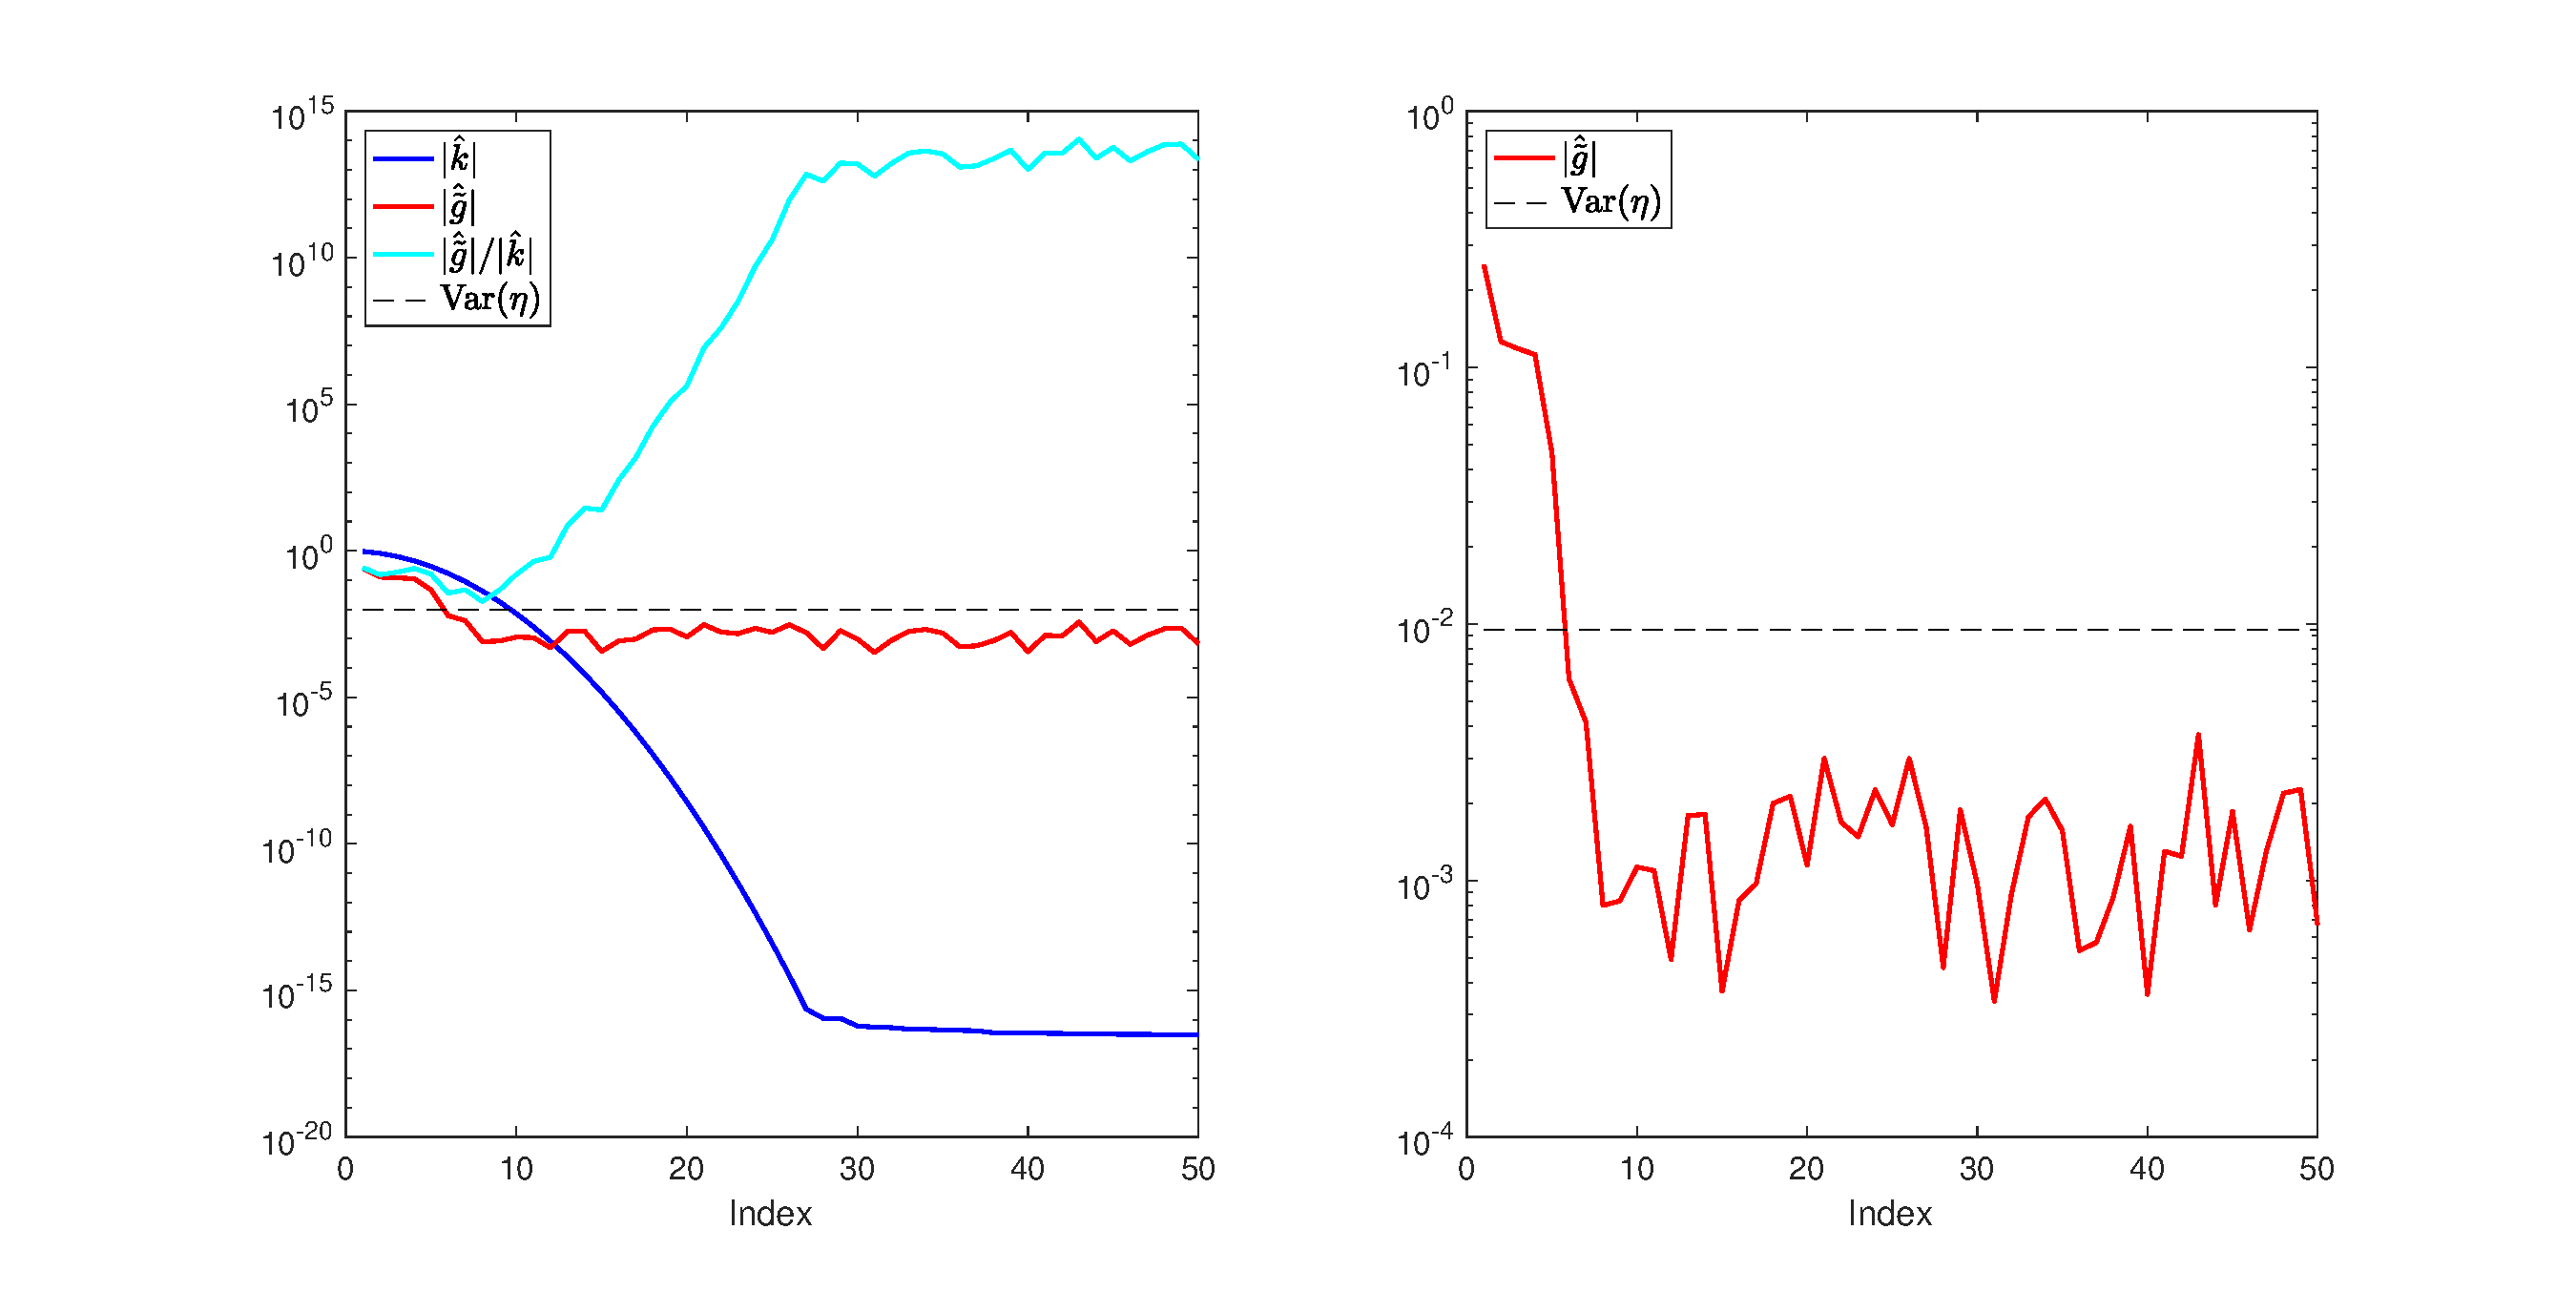
\includegraphics[scale = 0.45]{Figures/PicardPlot1D_F2_S15_W200.eps}}
\caption{(Left) A Picard plot generated from the second test function, a Gaussian blur with a width of 200, and an SNR of 15. The terms $|\dft{\gnoiseVec}_\ell|/|\dft{k}_\ell|$ decrease until index 8, at which case the terms increase in magnitude. This is due to the fact that the $|\dft{k}_\ell|$ steadily decrease, while the $|\dft{\gnoiseVec}_\ell|$ level off just below the variance in the noise. (Right) A zoom-in of the Picard plot is provided, showing that elements of the DFT of $\gnoiseVec$ decay only slightly below the variance of the noise in $\gnoiseVec$.}
\label{PicardPlot}
\end{figure}

While the connection between lines \eqref{eq:InvProdDFT} and \eqref{eq:ApproxSolDFT} and the SVD have been noted in regard to the structure of the terms and equations, a complete connection can be made if another property about $\kMat$ is assumed. Until this point $\kMat$ is assumed to be an invertible $N \times N$ circulant matrix formed from a vector $\kVec$. If $\kMat$ is also assumed to be symmetric, then the SVD of $\kMat$ is the same as the diagonalization by the unitary DFT matrix $F$ and the singular values of $\kMat$ are also the eigenvalues. \par 
Analogous to the DFT, the discrete cosine transform (DCT) can be introduced from the perspective of approximating the coefficients of a cosine series. Given a function $f(t)$ defined on the interval $[0,1]$, consider the even extension of $f_e(t)$ defined by
\[f_e(t) = \begin{cases}
f(t), & 0 \leq t \leq 1 \\
f(-t), & -1 \leq t < 0
\end{cases}.\]
From \cite[p.~49]{BoggessNarcowich2009}, the Fourier series expansion of $f_e(t)$ will only contain cosine terms and the coefficients of these terms are
\begin{align*}
a_0 &= \int_0^1 f(t)~dt, \\
a_j &= 2\int_0^1 f(t) \cos(j\pi{t})~dt, \quad j \leq 1.
\end{align*}
Approximating the integral for $a_j$ with $j \geq 1$ using the midpoint rule with $N$ subintervals of $[0,1]$ gives
\[a_j \approx \frac{2}{N}\sum_{k=0}^{N-1} f\left(\frac{1}{N}\left(k+\frac{1}{2}\right)\right)\cos\left(\frac{j\pi}{N}\left(k+\frac{1}{2}\right)\right).\]
Adjusting the scale factor and rewriting the argument of cosine yields the discrete transform. Given an $N$-vector $\mathbf{x}$ of real numbers, the discrete cosine transform (DCT) of $\mathbf{x}$, denoted $\dct{x}$, is defined as
\begin{equation}
\label{eq:DCT definition}
\dct{x}_j = \sqrt{\frac{2 - \delta_{j,0}}{N}} \sum_{k=0}^{N-1} x_k\cos\left(\frac{j\pi(2k + 1)}{2N}\right).
\end{equation}
Here $\delta_{j,0}$ is the Kronecker delta function, which in \eqref{eq:DCT definition} has the effect of introducing a factor of $1/\sqrt{N}$ in the zeroth component of $\dct{x}$ instead of $\sqrt{2}/\sqrt{N}$. The DCT matrix, denoted by $C$, has entries
\begin{equation}
\label{eq:DCT matrix}
C_{j,k} = \sqrt{\frac{2 - \delta_{j,0}}{N}} \cos\left(\frac{\pi{j}(2k + 1)}{2N}\right).
\end{equation}
By switching $j$ and $k$, it is clear that $C$ is not symmetric. However, $C$ is orthogonal which is analogous to the DFT matrix being unitary. Fortunately, many of the statistical results in Section \ref{ch:DCT of white noise} demonstrate that the statistics of the DCT of white noise are simpler that those of the DFT. Another benefit of the DCT is that the implied even boundary conditions ensure continuity at the endpoints in the continuous setting. \par
To fully describe the set of matrices diagonalized by the DCT, let the shift operator $\shift: \mathbb{R}^n \rightarrow \mathbb{R}^n$ be defined as
\[\shift(\mathbf{v}) = \trans{[v_1,v_2,\ldots,v_{n-1},0]}, \quad \mathbf{v} = \trans{[v_0,v_1,\ldots,v_{n-1}]} \in \mathbb{R}^n.\] 
The class of matrices diagonalization by the DCT can now be described.
\begin{theorem}[{{\cite{ChanChanWong,KailathOlshevsky1996,Martucci1994,Sanchez_et_al}}}]
\label{thm:DCT Diagonalization}
Let $\mathcal{C}$ be the class of matrices that can be diagonalized by the DCT matrix $C$. Then
\[\mathcal{C} = \{T(\mathbf{v}) + H\left(\shift(\mathbf{v})\right) ~|~ \mathbf{v} \in \mathbb{R}^n\}.\]
\end{theorem}
The diagonalization properties of the DCT in relation to Neumann boundary conditions can now be described.
\begin{theorem}
\label{thm:Neumann Diagonalization}
Let the kernel sequence \eqref{eq:Kernel seq.} satisfy $k_j = k_{-j}$ for all $j \in \mathbb{Z}$. Then the matrix $K$ in \eqref{eq:Neumann Kf = g} can be expressed as
\[K = T(\mathbf{u}) + H\left(\shift(\mathbf{u})\right),\]
where $\mathbf{u} = \trans{[k_0,k_1,\ldots,k_{m-1},0,\ldots,0]}$. In other words, $K$ can be diagonalized by the DCT.
\end{theorem}
\begin{proof}
Equation \eqref{eq:Neumann Kf = g} gives $K = [(0~|~T_{l})J + T + (T_{r}~|~0)J]$. Then $T = T(\mathbf{u})$ by the definition of $T$, and so it remains to show that $[(0~|~T_{l}) + (T_{r}~|~0)]J = H\left(\shift(\mathbf{u})\right)$. From the definitions of $T_{l}$ and $T_{r}$, the sum $(0~|~T_{l}) + (T_{r}~|~0)$ is equal to $T\left(J\shift(\mathbf{u})\right)$. Thus by Lemma \ref{lem:TJ = H},
\[[(0~|~T_{l}) + (T_{r}~|~0)]J = T\left(J\shift(\mathbf{u})\right)J = H\left(\shift(\mathbf{u})\right).\]
Therefore $K = T(\mathbf{u}) + H\left(\shift(\mathbf{u})\right)$, and Theorem \ref{thm:DCT Diagonalization} states that $K$ can be diagonalized by the DCT. 
\end{proof}

To conclude this section, the discrete sine transform (DST) will be briefly discussed. Given a function $f(t)$ defined on the interval $[0,1]$, consider the odd extension of $f_o(t)$ defined by
\[f_o(t) = \begin{cases}
f(t), & 0 \leq t \leq 1 \\
-f(-t), & -1 \leq t < 0
\end{cases}.\]
The Fourier series expansion of $f_o(t)$ will only contain sine terms and the coefficients of these terms are
\[b_j = 2\int_0^1 f(t) \sin((j+1)\pi{t})~dt, \quad j \geq 0.\]
The factor $j+1$ is so that the series does not always begin with a zero term; in other words, $b_0$ is not identically zero. Using the midpoint rule with $N$ subintervals gives
\[b_j \approx \frac{2}{N}\sum_{k=0}^{N-1} f\left(\frac{1}{N}\left(k+\frac{1}{2}\right)\right)\sin\left(\frac{(j+1)\pi}{N}\left(k+\frac{1}{2}\right)\right).\]
Again a modification of the scale factor and rewriting the argument of sine produces the discrete transform; the factor $j+1$ in the discrete transform ensures that the first DCT component $\dct{b}_0$ is not guaranteed to be zero. Unlike the DCT, however, the DST implies odd boundary conditions can produce discontinuities at the boundaries in the continuous setting. For this reason the DST will not be considered for the numerical examples.

\section{Downsampling and white noise} \label{sec:Downsampling and white noise}
While analysis has been conducted regarding the convergence of predictive and estimation error for Tikhonov regularization as the number of sample points becomes large \cite[p.~109-126]{Vogel:2002}, the effects of reducing the number of sample points must be explored. \par  
To formalize the concept of downsampling, consider $\mathbf{z} = [z_0,z_2,\ldots,z_{n-1}]$. Then a vector $\mathbf{y}$ is called a downsampling of $\mathbf{z}$ if $\mathbf{y} = [z_{n_0},z_{n_1},\ldots,z_{n_{m-1}}]$, where $m \leq n$ and $n_j:\{0,1,\ldots,{m-1}\}\rightarrow\{0,1,\ldots,{n-1}\}$ is a strictly increasing function. This definition is analogous to the definition of a subsequence except with a finite number of terms. \par
Theoretically, the variance of the noise vector does not change when a vector is downsampled because of the properties of variance. For any $m\times n$ matrix $M$ and $n$-vector $\noiseVec \sim \mathcal{N}(\zeroVec,\noiseSD^2I)$
\begin{equation}
\Var(M\noiseVec) = M\Var(\noiseVec)\trans{M} = \noiseSD^2MI\trans{M} = \noiseSD^2M\trans{M}
\label{eq:VarProp}
\end{equation}
where $M\trans{M}$ is an $m \times m$ matrix. Certainly for arbitrary $M$, $M\trans{M}$ can differ from an $m \times m$ identity matrix, which would mean that the new noise vector $M\noiseVec$ no longer represents white noise. However, given an $n$-vector $\noiseVec \sim \mathcal{N}(\zeroVec,\noiseSD^2I)$ and the goal of obtaining a downsampled version of $\noiseVec$, a matrix $E$ can be found such that $E\noiseVec$ is the downsampled vector. Since the DFT and DCT are utilized in the regularization process, a downsampled vector whose components are still equidistant from adjacent components is desirable. If the finest sampling $\tVec$ of the interval $[0,1]$ has $N = 2^L$ points, a natural downsampling with this property would be to select every other component of $\tVec$. The resulting downsampled vector would then have length $N/2 = 2^{L-1}$. A matrix $E$ that accomplishes this downsampling is the $N/2 \times N$ matrix defined as
\begin{equation}
E = [\mathbf{e}_0 \: \mathbf{0} \: \mathbf{e}_1 \: \mathbf{0} \: \mathbf{e}_2 \: \mathbf{0} \ldots \mathbf{e}_{N-2} \: \mathbf{0}]
\label{eq:Downsampling matrix}
\end{equation}
where $\mathbf{0}$ is the $N/2$-vector of all zeros and $\mathbf{e}_j$ is the $N/2$-vector of all zeros except for 1 as the $j\text{th}$ component, $0 \leq j \leq (N/2)-1$. Another explanation of how to construct $E$ is to concatenate every other row of an $N \times N$ identity matrix. In an effort to clarify this downsampling process, let $\tVec^{n}$ denote the $n$-point downsampling of $\tVec$. Then with this new notation, $\tVec^{N/2} = E\tVec$. \par
As an example, consider the vector
\[\tVec = \trans{\begin{bmatrix}
0 & \dfrac{1}{8} & \dfrac{1}{4} & \dfrac{3}{8} & \dfrac{1}{2} & \dfrac{5}{8} & \dfrac{3}{4} & \dfrac{7}{8}
\end{bmatrix}},\]
which is an equispaced 8-point discretization of $[0,1]$. The $4 \times 8$ matrix $E$ used to obtain downsampling $\tVec^{4}$ is
\[E = \begin{bmatrix}
1 & 0 & 0 & 0 & 0 & 0 & 0 & 0 \\
0 & 0 & 1 & 0 & 0 & 0 & 0 & 0 \\
0 & 0 & 0 & 0 & 1 & 0 & 0 & 0 \\
0 & 0 & 0 & 0 & 0 & 0 & 1 & 0 \\
\end{bmatrix}.\]
Then $\tVec^4$ obtained by the product $E\tVec$ has equispaced components as desired:
\[\tVec^4 = E\tVec = \trans{\begin{bmatrix}
0 & \dfrac{1}{4} & \dfrac{1}{2} & \dfrac{3}{4}
\end{bmatrix}}.\]
\indent Another property of the $N/2 \times N$ matrix $E$ defined in \eqref{eq:Downsampling matrix} is that $E\trans{E} = I$, where $I$ is the $N/2 \times N/2$ identity matrix.  This is a direct consequence of $\mathbf{e}_j\trans{\mathbf{e}}_j = 1$ for all $j$ with $0 \leq j \leq (N/2)-1$. Using the property in \eqref{eq:VarProp}, the variance of the  noise vector $\noiseVec^{N/2}$ downsampled from $\noiseVec$ is then
\[\Var(\noiseVec^{N/2}) = \Var(E\noiseVec) = E\Var(\noiseVec)\trans{E} = \noiseSD^2E\trans{E} = \noiseSD^2I\]
where $I$ is the $N/2 \times N/2$ identity matrix. Therefore, downsampling white noise vectors in this way produces white noise vectors of half length, theoretically preserving variance across downsamples. As a final remark, the process of downsampling described here can be used to obtain downsampled vectors of length $N/(2^2), N/(2^3), \ldots, N/N$, though the final resolution has been chosen as $N/(2^8) = 16$. \par
While the variance of the noise is preserved across downsampling resolution in theory, numerically there is some fluctuation. As the downsampling resolutions decrease, i.e. the length of the downsampled vectors decreases, the sample variances more spread out. Figure \ref{VarPlot1D} demonstrates this phenomenon by showing boxplots of sample variance versus downsampling resolutions. %\newpage

\begin{figure}[htb]
\centerline{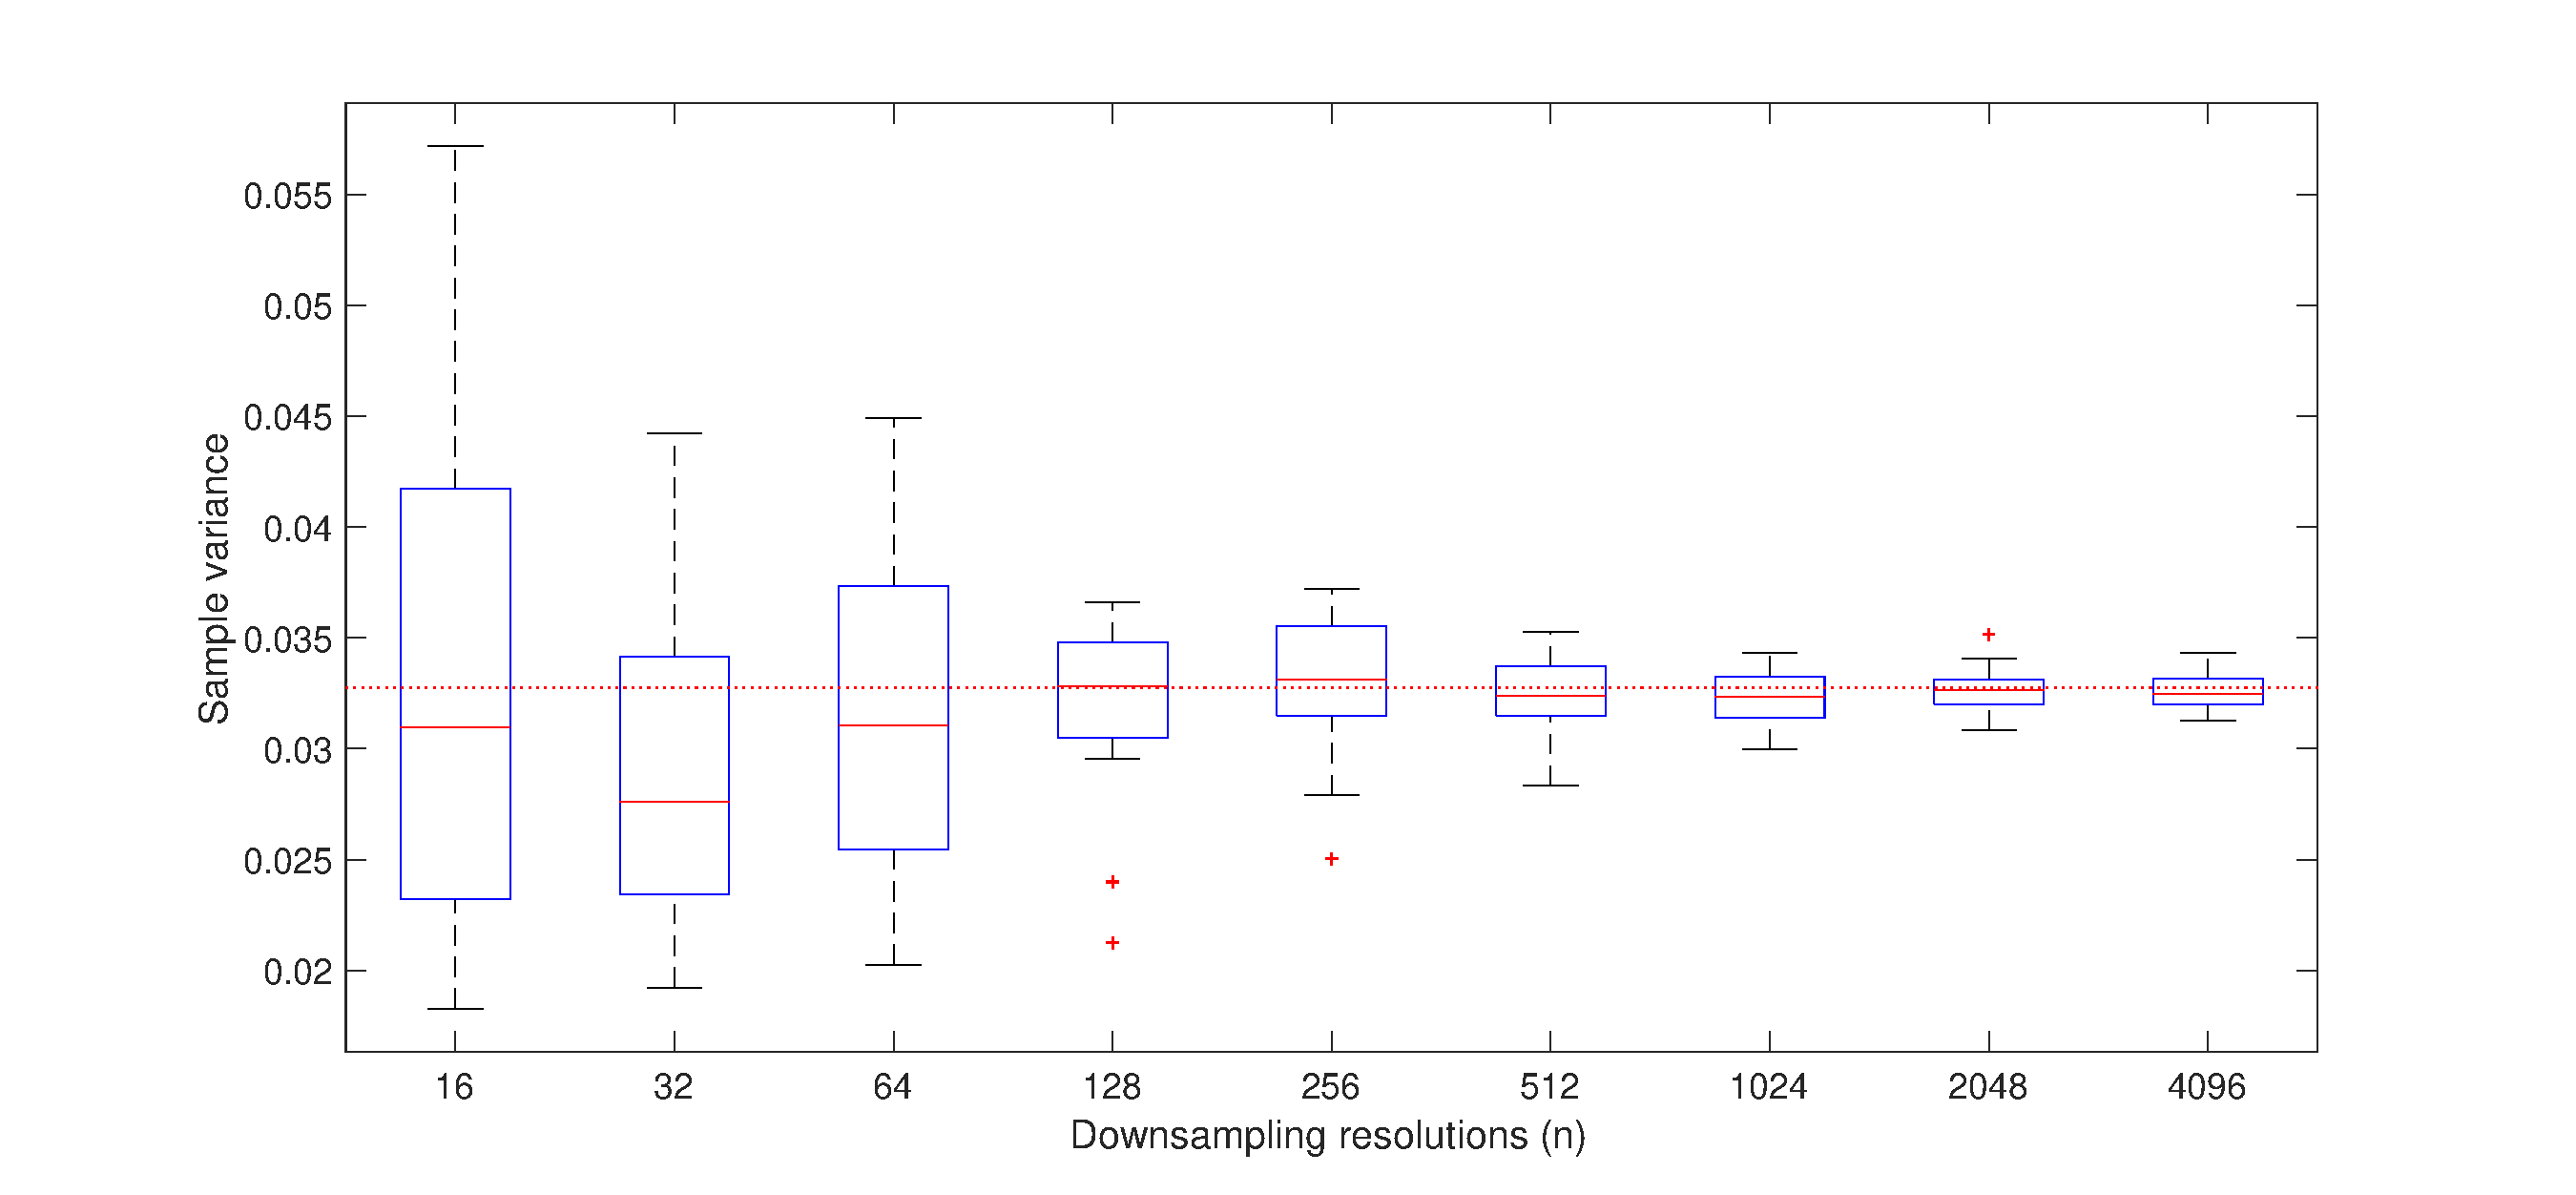
\includegraphics[scale=0.45]{Figures/VarPlot1D_F1_S05_W100_R20.eps}}
\caption{The boxplots were generated from the sample variances of downsampled noise vectors. The theoretical variance of the noise was set to 0.0327, which is indicated by the horizontal dotted line. This figure illustrates that as the lengths of the downsampled vectors decrease, the variance in the computed sample variances increases.}
\label{VarPlot1D}
\end{figure}

One description of the effects of downsampling a vector in terms of the DFT is the Downsampling Theorem \cite[Ch.~7]{AudioDFT}. Given a vector $\mathbf{x} \in \mathbb{C}^N$, where $N = LM$ for positive integers $L$ and $M$, and \textit{aliasing operator} $\alias_L(\cdot) : \mathbb{C}^N \rightarrow \mathbb{C}^M$ is defined as
\[\left(\alias_L(\mathbf{x})\right)_j = \sum_{k=0}^{L-1} x_{j+kM}, \quad \mathbf{x} \in \mathbb{C}^N, \quad j \in \{0,1,\ldots,M-1\}.\]
The vector $\alias_L(\mathbf{x})$ is is the result of partitioning the vector $\mathbf{x}$ into $L$ vectors of length $M$ and summing them. The aliasing operator is linear and thus could be defined using a matrix representation; if $L = 2$, the aliasing operator has an $M \times N$ matrix representation $A$ that has entries
\[A_{j,k} = \begin{cases}
1, & j = k \bmod M, \\
0, & \text{otherwise}
\end{cases}, \quad 0 \leq j \leq M-1, ~ 0 \leq k \leq N-1.\]
With the aliasing operator defined, the Downsampling Theorem can be stated.
\begin{theorem}{Downsampling Theorem}
Let $\mathbf{x} \in \mathbb{C}^N$, where $N = LM$ for positive integers $L$ and $M$, let $\mathbf{y} = \mathbf{x}^M$, and let $\dft{y}$ and $\dft{x}$ denote the DFT of $\mathbf{y}$ and $\mathbf{x}$, respectively. Then
\[\dft{\mathbf{y}} = \frac{1}{\sqrt{L}}\alias_L\left(\dft{\mathbf{x}}\right).\]
\end{theorem}
\begin{proof}
Since the length of $\dft{\mathbf{x}}$ is $N$, $\alias_L\left(\dft{\mathbf{x}}\right)$ has length $M = N/L$. Letting $\mathbf{z} = \alias\left(\dft{\mathbf{x}}\right)$, we have that
\[z_j = \sum_{k=0}^{L-1}\dft{x}_{j+kM}, \quad j\in\{0,1,\ldots,M-1\},\]
because each component of $\mathbf{z}$ is the sum of $L$ components of $\dft{\mathbf{x}}$. Fixing some $j\in\{0,1,\ldots,M-1\}$, the definition of the DFT and the fact that $M/N = L$ give
\begin{align*}
\sum_{k=0}^{L-1}\dft{x}_{j+kM} &= \sum_{k=0}^{L-1} \left(\frac{1}{\sqrt{N}}\sum_{\ell=0}^{N-1} x_{\ell}\exp\left(\frac{-2\pi{i}(j+kM)\ell}{N}\right)\right) \\
&= \frac{1}{\sqrt{N}} \sum_{k=0}^{L-1} \sum_{\ell=0}^{N-1} x_{\ell}\exp\left(\frac{-2\pi{ij\ell}}{N}\right)\exp\left(\frac{-2\pi{ikM\ell}}{N}\right) \\
&= \frac{1}{\sqrt{N}} \sum_{k=0}^{L-1} \sum_{\ell=0}^{N-1} x_{\ell}\exp\left(\frac{-2\pi{ij\ell}}{N}\right)\exp\left(\frac{-2\pi{ik\ell}}{L}\right) \\
&= \frac{1}{\sqrt{N}} \sum_{\ell=0}^{N-1} x_{\ell} \exp\left(\frac{-2\pi{ij\ell}}{N}\right) \left(\sum_{k=0}^{L-1} \exp\left(\frac{-2\pi{ik\ell}}{L}\right)\right).
\end{align*}
The sum over $k$ is geometric:
\[\sum_{k=0}^{L-1} \exp\left(\frac{-2\pi{ik\ell}}{L}\right) = \sum_{k=0}^{L-1} \left(\exp\left(\frac{-2\pi{i\ell}}{L}\right)\right)^k.\]
If $n = 0 \bmod L$, then the summands are all 1 and the sum is equal to $L$. If $n \neq 0 \bmod L$, then the formula for a geometric sum produces
\[\sum_{k=0}^{L-1} \left(\exp\left(\frac{-2\pi{i\ell}}{L}\right)\right)^k = \frac{1-\exp(-2\pi{i\ell})}{1-\exp(-2\pi{i\ell/L})} = 0,\]
where the last equality comes from noting that $\exp(-2\pi{i\ell}) = 1$ for all integers $\ell$. Performing the change of index $m = \ell/L$, the results regarding the sum over $k$ imply
\[\frac{1}{\sqrt{N}} \sum_{\ell=0}^{N-1} x_{\ell} \exp\left(\frac{-2\pi{ij\ell}}{N}\right) \left(\sum_{k=0}^{L-1} \exp\left(\frac{-2\pi{ik\ell}}{L}\right)\right) = \frac{L}{\sqrt{N}} \sum_{m=0}^{(N/L)-1} x_{mL} \exp\left(\frac{-2\pi{ijmL}}{N}\right)\]
because integral values of $m = \ell/L$ means that $\ell = 0 \bmod L$. Using $N = LM$ and noting that $x_{mL} = y_m$ yields
\[z_j = \frac{L}{\sqrt{N}} \sum_{m=0}^{(N/L)-1} x_{mL} \exp\left(\frac{-2\pi{ijmL}}{N}\right) = \frac{L}{\sqrt{N}} \sum_{m=0}^{M-1} y_m \exp\left(\frac{-2\pi{ijm}}{M}\right) = \frac{L\sqrt{M}}{\sqrt{N}} \dft{y}_j.\]
Therefore $\dft{\mathbf{y}} = \frac{1}{\sqrt{L}}\mathbf{z} = \frac{1}{\sqrt{L}}\alias_L\left(\dft{\mathbf{x}}\right)$.
\end{proof}
In words, the Downsampling Theorem states that the DFT of a downsampled vector is equal to a (scaled) summed partition of the DFT of the original vector. A direction of future work will be to see if the Downsampling Theorem can be directly applied to the parameter estimation functions in Chapter \ref{ch:Parameter estimation methods} to analyze the effects of downsampling on the functions themselves. \par 
Each function in Chapter \ref{ch:Parameter estimation methods} uses the assumption that noise is present in the given data. Since data in the context of the DFT are often considered discretizations of analog signals, a common quantifier of noise in data is the signal-to-noise ratio (SNR). Though the definition of SNR varies, the definition chosen for this investigation is
\begin{equation}
\label{eq:SNR}
\text{SNR} = 10\log_{10}\left(\frac{P_{\text{signal}}}{P_{\text{noise}}}\right)
\end{equation}
where $P$ denotes average power. In the discrete setting, the average power of a signal $\mathbf{f}$ of length $N$ is defined as $\|\mathbf{f}\|^2/N$. Using this definition, $P_{\text{signal}} = \|\gVec\|^2/N$ and $P_{\text{noise}} = \|\noiseVec\|^2/N$ and so the quotient in the logarithm is $\|\gVec\|^2/\|\noiseVec\|^2$. The quotient can also be expressed as $(\|\gVec\|/\|\gnoiseVec - \gVec\|)^2$, which is the square of the multiplicative inverse of the relative error of $\gnoiseVec$. \par
In MATLAB, the noise vector $\noiseVec$ can be constructed by first taking an $N$-vector $\mathbf{e}$ drawn from the multivariate standard normal distribution and multiplying the vector by a constant $\noiseSD$. Doing so ensures that $\noiseVec$ has variance $\noiseSD^2$ because $\Var(\noise) = \Var(\noiseSD\:\mathbf{e}) = \noiseSD^2\:\Var(\mathbf{e})$ and $\mathbf{e}$ has unit variance. Thus it is useful to rearrange the equation defining SNR into an equation that provides a way of finding the necessary variance for a given SNR value. The rearrangement is shown below, with $\|\noiseVec\|^2$ replaced by $\E(\|\noiseVec\|^2)$.
\[\E(\|\noiseVec\|^2) = \frac{\|\gVec\|^2}{10^{(\text{SNR}/10)}}\]
Using the properties of expected value and the fact that $\E(\|\noiseVec\|^2) = \E(\|\noiseSD\:\mathbf{e}\|^2)$, the term on the left hand side of the equation can be changed as
\[\E(\|\noiseVec\|^2) = \E(\|\noiseSD\:\mathbf{e}\|^2) = \noiseSD^2 \sum_{j=1}^N \E(\mathbf{e}_i^2) = \noiseSD^2 \sum_{j=1}^N \left(\E(\mathbf{e}_i)^2 + \Var(\mathbf{e}_i)\right) = \noiseSD^2 \sum_{j=1}^N \left(0^2 + 1\right) = \noiseSD^2\:N.\]
Utilizing this change, the following equation for variance is obtained.
\begin{equation}
\label{eq:Var}
\noiseSD^2 = \frac{\|\gVec\|^2}{N \cdot 10^{(\text{SNR}/10)}}
\end{equation}
This equation is used for the numerical construction of the noise vectors. SNR values of 5 and 25 are used to generate the white noise added to $\gVec$, and one such data realization is shown in Figure \ref{NoisePlot1D_F2_S05_W200}. \par

\begin{figure}
	\centerline{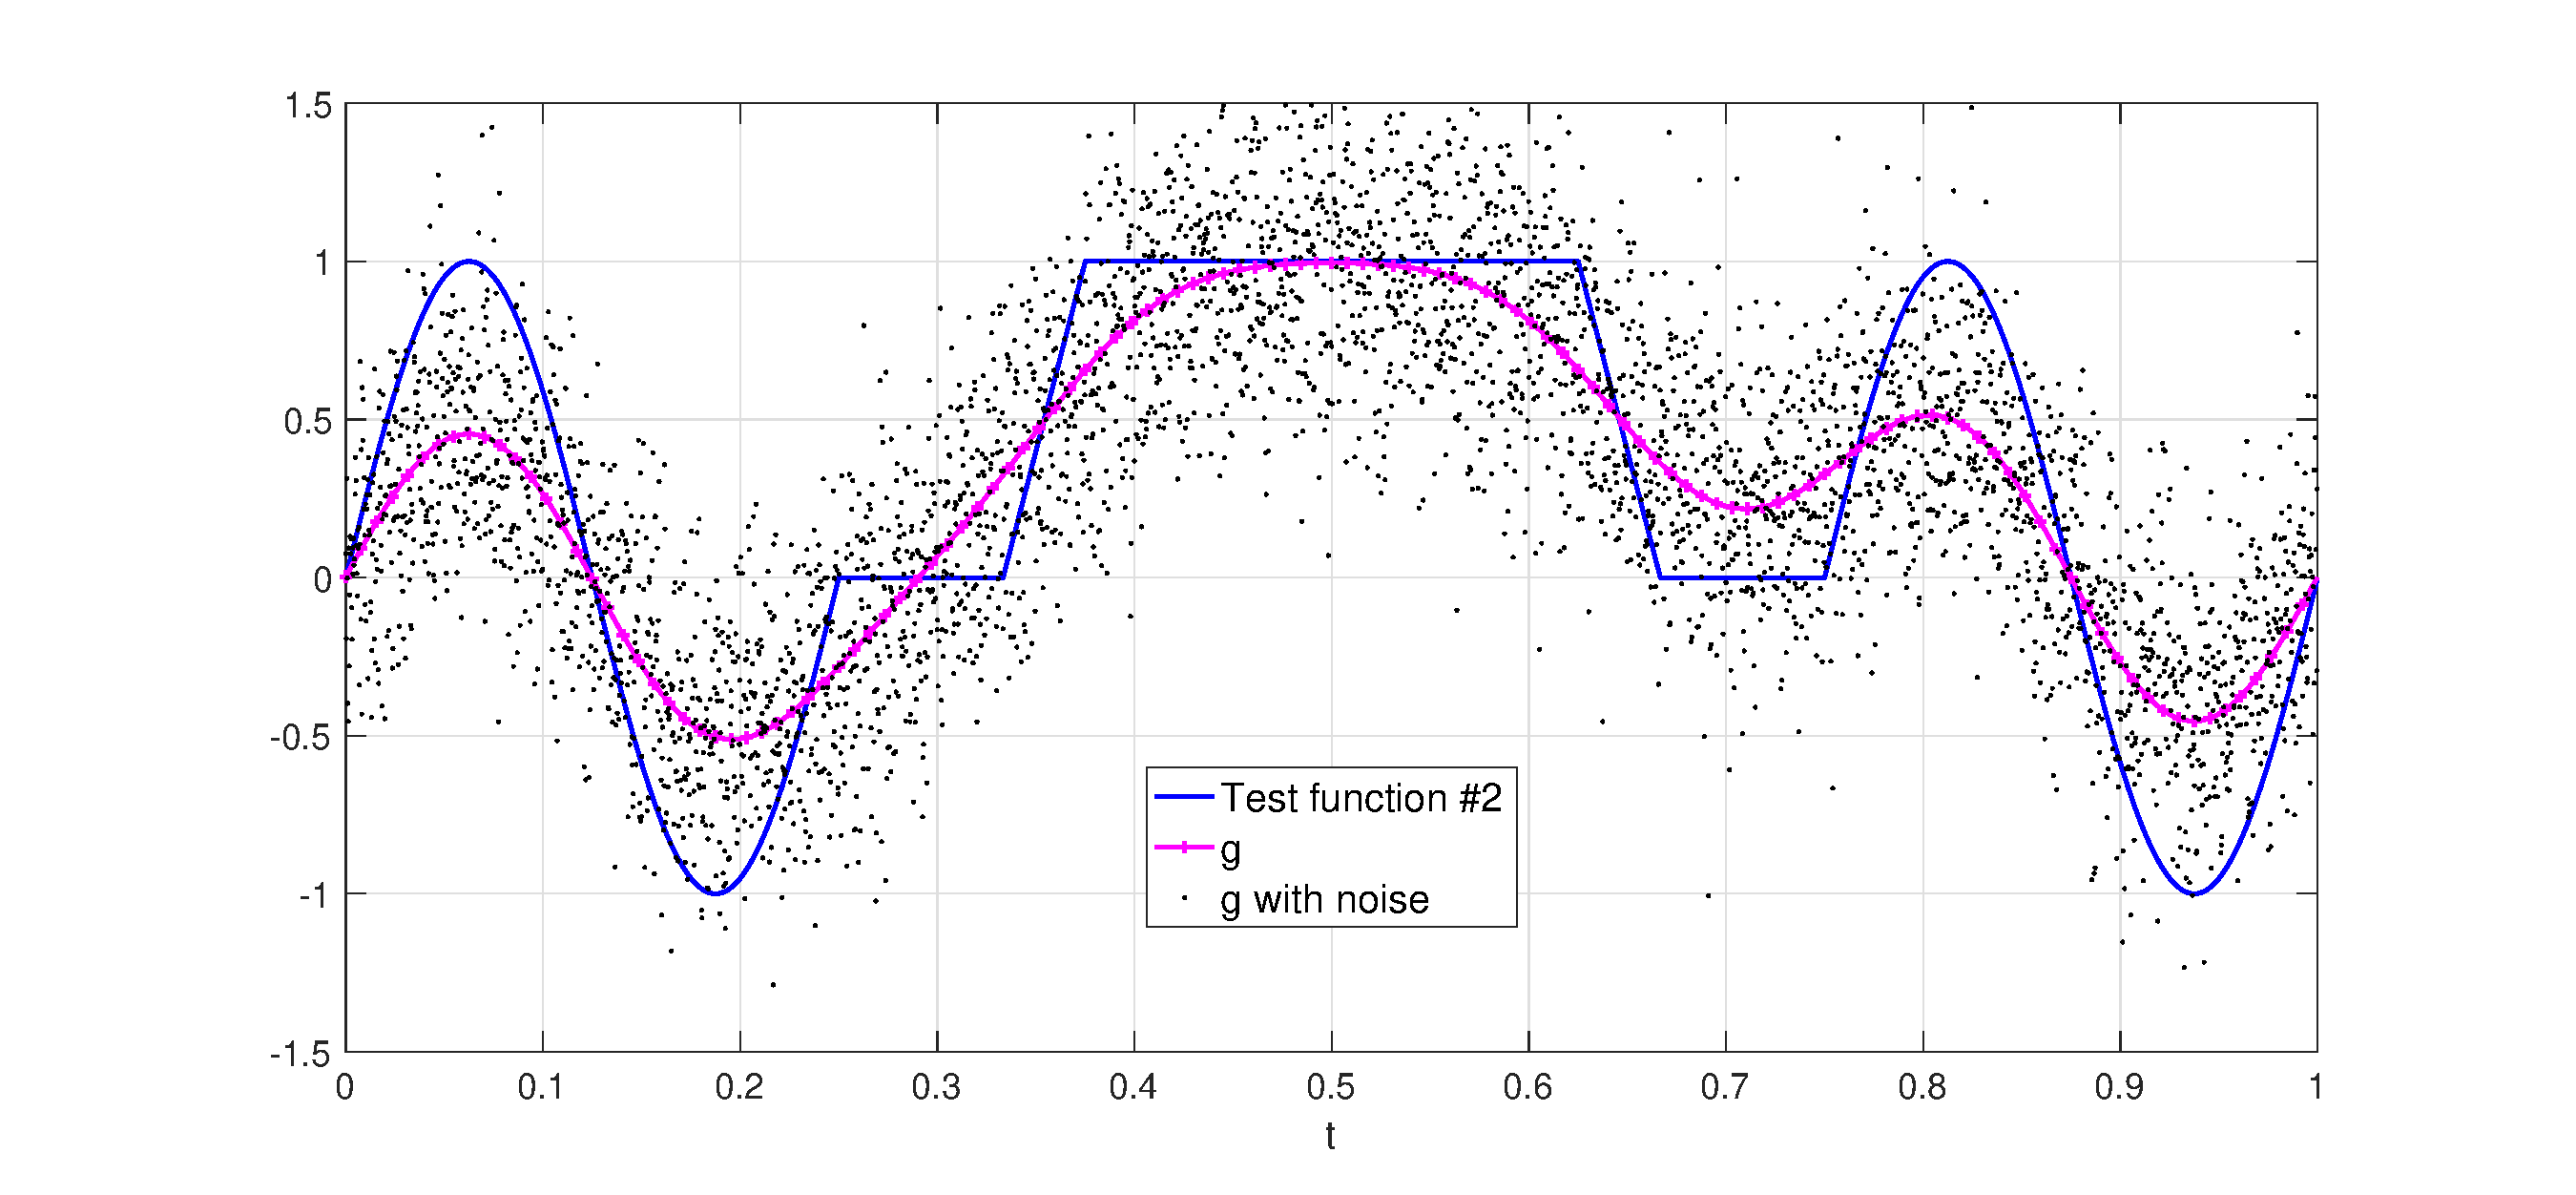
\includegraphics[scale = 0.45]{Figures/NoisePlot1D_F2_S05_W200.eps}}
\caption{The plot shows one data realization of $\gVec$ with noise, where the original function $f$ was the second test function. The SNR value is 5 and the width of the Gaussian kernel is 200.}
\label{NoisePlot1D_F2_S05_W200}
\end{figure}

For an accurate evaluation of the numerical examples and their results, multiple realizations of noise are used. A primary advantage of multiple noise realizations is that the sample variance of noise vectors approaches the desired variance as the number of realizations increases. More rigorously, the mean of the sample variances of the noise vectors converges almost surely to the expected value of the sample variance, which is the desired variance $\noiseSD^2$; this is a direct consequence of the (strong) law of large numbers and the fact that the noise vectors are independent and identically distributed with standard normal distribution.

\chapter{Statistical considerations} \label{ch:Stats}

Since the parameter estimation methods in Chapter \ref{ch:Parameter estimation methods} involve DFT's and DCT's of the vector $\gnoiseVec = \gVec + \noiseVec$, some results regarding the distribution of the components of $\dft{\noiseVec}$ and $\dct{\noiseVec}$ will be presented. Since the DFT is a map from $\mathbb{C}^n$ to $\mathbb{C}^n$ and $\noiseVec$ is assumed to be a realization of a real random vector, some effort is necessary to carefully examine the distribution of the components of $\dft{\noiseVec}$. In contrast, the DCT (and DST) is a map from $\mathbb{R}^n$ to $\mathbb{R}^n$, so the statistics regarding the DCT of white noise are more straightforward.

\section{DFT of white noise} \label{ch:DFT of white noise}
The first results will be in regard to the real and imaginary parts of the $\dft{\noiseVec}$. Letting $A$ and $B$ be the real and imaginary parts, respectively, of the $n \times n$ DFT matrix, Euler's identity gives
\begin{equation}
A_{j,k} = \frac{1}{\sqrt{n}}\cos\left(\frac{-2\pi{jk}}{n}\right), \quad B_{j,k} = \frac{1}{\sqrt{n}}\sin\left(\frac{-2\pi{jk}}{n}\right),
\label{eq:Components Re(F) and Im(F)}
\end{equation}
for $0 \leq j,k \leq n-1$. It is clear from \eqref{eq:Components Re(F) and Im(F)} that the matrices $A$ and $B$ are symmetric. The rows (and by symmetry, columns) of $A$ and $B$ have the following orthogonality properties. For compactness, let $\mathbf{e}_j$ denote the $n$-vector with 1 as the $j$th component and zeros elsewhere and let $J$ denote the $n \times n$ exchange matrix.
\begin{lemma}
\label{lem:Inner products}
Let $A$ and $B$ be the real and imaginary parts, respectively, of the $n \times n$ DFT matrix, and let $\langle\cdot,\cdot\rangle$ denote standard inner product (dot product) of $\mathbb{R}^n$. Then for $0 \leq j,k \leq n-1$:
\begin{enumerate}
\item $\langle A_{j,\cdot}, B_{k,\cdot}\rangle = 0$.
\item If $n$ is even, then 
\begin{align*}
\langle A_{j,\cdot}, A_{k,\cdot}\rangle &= \begin{cases}
1 & j = k = 0 \text{ or } j = k = n/2 \\ 
1/2 & j = k \neq 0 \text{ or } j = k \neq n/2 \\ 
1/2 & j \neq k \text{ and } k = n - j \\ 
0 & \text{otherwise} \end{cases}, \\
\langle B_{j,\cdot}, B_{k,\cdot}\rangle &= \begin{cases}
0 & j = k = 0 \text{ or } j = k = n/2 \\ 
1/2 & j = k \neq 0 \text{ or } j = k \neq n/2 \\ 
-1/2 &  j \neq k \text{ and } k = n - j \\ 
0 & \text{otherwise} \end{cases}.
\end{align*}
Equivalently,
\[A\trans{A} = \frac{1}{2}I + \frac{1}{2}\left(\mathbf{e}_0\trans{\mathbf{e}}_0 + \mathbf{e}_{n/2}\trans{\mathbf{e}}_{n/2} + J\right), \quad B\trans{B} = \frac{1}{2}I - \frac{1}{2}\left(\mathbf{e}_0\trans{\mathbf{e}}_0 + \mathbf{e}_{n/2}\trans{\mathbf{e}}_{n/2} + J\right).\]
\item If $n$ is odd, then
\[\langle A_{j,\cdot}, A_{k,\cdot}\rangle = \begin{cases}
1 & j = k = 0 \\ 
1/2 & j = k \neq 0 \\
1/2 & j+k = n \\
0 & \text{otherwise} \end{cases}, \quad 
\langle B_{j,\cdot}, B_{k,\cdot}\rangle = \begin{cases}
0 & j = k = 0 \\ 
1/2 & j = k \neq 0 \\
-1/2 & j+k = n \\
0 & \text{otherwise} \end{cases}.\]
Equivalently,
\[A\trans{A} = \frac{1}{2}I + \frac{1}{2}\left(\mathbf{e}_0\trans{\mathbf{e}}_0 + J\right), \quad B\trans{B} = \frac{1}{2}I - \frac{1}{2}\left(\mathbf{e}_0\trans{\mathbf{e}}_0 + J\right).\]
\end{enumerate}
Notice that in both the even and odd cases, $A\trans{A} + B\trans{B} = I$.
\end{lemma}
\begin{proof}
Property (i) will first be established. Letting $A$ and $B$ be as required, \eqref{eq:Components Re(F) and Im(F)} gives
\begin{equation}
\langle A_{j,\cdot}, B_{k,\cdot}\rangle = \frac{1}{n}\sum_{\ell=0}^{n-1}\cos\left(\frac{-2\pi{j\ell}}{n}\right)\sin\left(\frac{-2\pi{\ell{k}}}{n}\right) = \frac{1}{n}\sum_{\ell=0}^{n-1}\cos\left(-\theta_{j\ell}\right)\sin\left(-\theta_{k\ell}\right),
\label{eq: <Re(F),Im(F)>}
\end{equation}
where $\theta_{j\ell} = 2\pi{j\ell}/n$. Applying the appropriate product-to-sum trigonometric identity and using the fact that sine is an odd function allows for the sum in \eqref{eq: <Re(F),Im(F)>} to be evaluated as
\begin{align*}
\frac{1}{n}\sum_{\ell=0}^{n-1}\cos\left(-\theta_{j\ell}\right)\sin\left(-\theta_{k\ell}\right) &= \frac{1}{2n}\sum_{\ell=0}^{n-1}\left[\sin\left(-\theta_{(j+k)\ell}\right) - \sin\left(-\theta_{(k-j)\ell}\right)\right] \\
&= \frac{1}{2n}\sum_{\ell=0}^{n-1}\left[\sin\left(\theta_{(k-j)\ell}\right) - \sin\left(\theta_{(j+k)\ell}\right)\right] \\
&= \frac{1}{2n}\left(s_1 - s_2\right),
\end{align*}
where
\[s_1 = \sum_{\ell=0}^{n-1}\sin\left(\theta_{(k-j)\ell}\right), \quad s_2 = \sum_{\ell=0}^{n-1}\sin\left(\theta_{(j+k)\ell}\right).\]
Both $s_1$ and $s_2$ are of the form $\sum_{\ell=0}^{n-1} \sin(\theta_{p\ell})$, where $p$ is an integer (either $k-j$ or $j+k$). This form can be written as
\[\sum_{\ell=0}^{n-1} \sin\left(\theta_{p\ell}\right) = \Im\left(\sum_{\ell=0}^{n-1} \exp\left(i\theta_{p\ell}\right)\right).\] 
If $p$ is a multiple of $n$, then $p = mn$ for some $m \in \mathbb{Z}$. Thus $\exp(i\theta_{p\ell}) = \exp(i2\pi{mn}\ell/n) = \exp(i2\pi{m\ell}) = 1$, and so
\[\Im\left(\sum_{\ell=0}^{n-1} \exp\left(i\theta_{p\ell}\right)\right) = \Im\left(\sum_{\ell=0}^{n-1} 1\right) = 0.\]
If $p$ is not a multiple of $n$, then
\[\Im\left(\sum_{\ell=0}^{n-1} \exp\left(i\theta_{p\ell}\right)\right) = \Im\left(\frac{1-\exp(i\theta_{np})}{1-\exp(i\theta_p)}\right).\]
However, $\theta_{np} = 2\pi{np}/n = 2\pi{p}$. Since $p$ is an integer, $\exp(i\theta_{np})  =\exp(i2\pi{p}) = 1$, meaning that the preceding equation is equal to zero. Therefore
\begin{align*}
s_1 &= \sum_{\ell=0}^{n-1}\sin\left(\theta_{(k-j)\ell}\right) = \Im\left(\sum_{\ell=0}^{n-1}\exp\left(i\theta_{(k-j)\ell}\right)\right) = 0, \\
s_2 &= \sum_{\ell=0}^{n-1}\sin\left(\theta_{(j+k)\ell}\right) = \Im\left(\sum_{\ell=0}^{n-1}\exp\left(i\theta_{(j+k)\ell}\right)\right) = 0
\end{align*}
for all $0 \leq j,k \leq n-1$, which implies $\langle A_{j,\cdot},B_{k,\cdot}\rangle = (s_1 - s_2)/2n = 0$. \par 
The results of properties (ii) and (iii) regarding $A$ will now be proved; the results regarding $B$ will be handled afterwards. Utilizing \eqref{eq:Components Re(F) and Im(F)} again,
\[\langle A_{j,\cdot}, A_{k,\cdot}\rangle = \frac{1}{n}\sum_{\ell=0}^{n-1}\cos\left(\frac{-2\pi{j\ell}}{n}\right)\cos\left(\frac{-2\pi{\ell{k}}}{n}\right) = \frac{1}{n}\sum_{\ell=0}^{n-1}\cos\left(-\theta_{j\ell}\right)\cos\left(-\theta_{k\ell}\right).\]
By the fact that cosine is an even function and applying another product-to-sum identity gives $\langle A_{j\cdot}, A_{k\cdot}\rangle = (c_1 + c_2)/2n$, where
\begin{equation}
c_1 = \sum_{\ell=0}^{n-1}\cos\left(\theta_{(j-k)\ell}\right), \quad c_2 = \sum_{\ell=0}^{n-1}\cos\left(\theta_{(j+k)\ell}\right).
\label{eq:c_1 and c_2}
\end{equation} 
Both $c_1$ and $c_2$ are of the form $\sum_{\ell=0}^{n-1} \cos(\theta_{p\ell})$, where $p$ is an integer (either $j-k$ or $j+k$). This form can be written as
\[\sum_{\ell=0}^{n-1} \cos\left(\theta_{p\ell}\right) = \Re\left(\sum_{\ell=0}^{n-1} \exp\left(i\theta_{p\ell}\right)\right).\] 
If $p$ is a multiple of $n$, then $p = mn$ for some $m \in \mathbb{Z}$. Thus $\exp(i\theta_{p\ell}) = \exp(i2\pi{mn}\ell/n) = \exp(i2\pi{m\ell}) = 1$, and so
\[\Re\left(\sum_{\ell=0}^{n-1} \exp\left(i\theta_{p\ell}\right)\right) = \Re\left(\sum_{\ell=0}^{n-1} 1\right) = n.\]
If $p$ is not a multiple of $n$, then
\[\Re\left(\sum_{\ell=0}^{n-1} \exp\left(i\theta_{p\ell}\right)\right) = \Re\left(\frac{1-\exp(i\theta_{np})}{1-\exp(i\theta_p)}\right).\]
However, $\theta_{np} = 2\pi{np}/n = 2\pi{p}$. Since $p$ is an integer, $\exp(i\theta_{np})  =\exp(i2\pi{p}) = 1$, meaning that the preceding equation is equal to zero. Thus 0 and $n$ are the two possible values of $c_1$ and $c_2$, which depend upon whether or not $j-k$ and $j+k$ are multiples of $n$. \par 
First consider property (ii), the case where $n$ is even.
\begin{itemize}
\item If $j = k = 0$ or $j = k = n/2$, then $j-k = 0$ and $j+k$ is either 0 or $n$. In other words, both $j-k$ and $j+k$ are multiples of $n$, and so $c_1 = c_2 = n$. This implies that $\langle A_{j,\cdot},A_{k,\cdot} \rangle = (c_1 + c_2)/2n = (n+n)/2n = 1$.
\item If $j = k \neq 0$ or $j = k \neq n/2$, then $j-k = 0$ but $j+k$ is not a multiple of $n$. Thus $c_1 = n$ and $c_2 = 0$, and so $\langle A_{j,\cdot},A_{k,\cdot} \rangle = (c_1 + c_2)/2n = (n+0)/2n = 1/2$.
\item If $j \neq k$ and $k = n-j$, then $j-k$ is not a multiple of $n$ but $j+k = n$. Thus $c_1 = 0$ and $c_2 = n$, and so $\langle A_{j,\cdot},A_{k,\cdot} \rangle = (c_1 + c_2)/2n = (0+n)/2n = 1/2$.
\item If $j \neq k$ and $k \neq n-j$, then neither $j-k$ nor $j+k$ are multiples of $n$. Thus $c_1 = c_2 = 0$, and so $\langle A_{j,\cdot},A_{k,\cdot} \rangle = (c_1 + c_2)/2n = (0+0)/2n = 0$.
\end{itemize}
For property (iii), the case where $n$ is odd, $n/2$ need not be considered and the preceding argument holds. \par 
For the results regarding $B$,
\[\langle B_{j,\cdot}, B_{k,\cdot} \rangle = \frac{1}{n}\sum_{\ell=0}^{n-1}\sin\left(\frac{-2\pi{j\ell}}{n}\right)\sin\left(\frac{-2\pi{\ell{k}}}{n}\right) = \frac{1}{n}\sum_{\ell=0}^{n-1}\sin\left(-\theta_{j\ell}\right)\sin\left(-\theta_{k\ell}\right).\]
By the fact that sine is an odd function and applying another product-to-sum identity gives $\langle B_{j,\cdot}, B_{k,\cdot}\rangle = (c_1 - c_2)/2n$, where $c_1$ and $c_2$ are defined by \eqref{eq:c_1 and c_2}. Again 0 and $n$ are the two possible values of $c_1$ and $c_2$, which depend upon whether or not $j-k$ and $j+k$ are multiples of $n$. \par 
First consider property (ii), the case where $n$ is even.
\begin{itemize}
\item If $j = k = 0$ or $j = k = n/2$, then $j-k = 0$ and $j+k$ is either 0 or $n$. In other words, both $j-k$ and $j+k$ are multiples of $n$, and so $c_1 = c_2 = n$. This implies that $\langle B_{j,\cdot},B_{k,\cdot} \rangle = (c_1 - c_2)/2n = (n-n)/2n = 0$.
\item If $j = k \neq 0$ or $j = k \neq n/2$, then $j-k = 0$ but $j+k$ is not a multiple of $n$. Thus $c_1 = n$ and $c_2 = 0$, and so $\langle B_{j,\cdot},B_{k,\cdot} \rangle = (c_1 - c_2)/2n = (n-0)/2n = 1/2$.
\item If $j \neq k$ and $k = n-j$, then $j-k$ is not a multiple of $n$ but $j+k = n$. Thus $c_1 = 0$ and $c_2 = n$, and so $\langle B_{j,\cdot},B_{k,\cdot} \rangle = (c_1 - c_2)/2n = (0-n)/2n = -1/2$.
\item If $j \neq k$ and $k \neq n-j$, then neither $j-k$ nor $j+k$ are multiples of $n$. Thus $c_1 = c_2 = 0$, and so $\langle B_{j,\cdot},B_{k,\cdot} \rangle = (c_1 - c_2)/2n = (0+0)/2n = 0$.
\end{itemize}
For property (iii), the case where $n$ is odd, $n/2$ need not be considered and again the preceding argument holds.
\end{proof}

There are some important consequences of Lemma \ref{lem:Inner products}. First, it provides a means to visualize the structure of the matrices $A^2 = A\trans{A}$ and $B^2 = B\trans{B}$. For example, if $n = 6$ then the matrices $A^2$ and $B^2$ are
\[A^2 = \begin{bmatrix}
1 & 0 & 0 & 0 & 0 & 0 \\
0 & \frac{1}{2} & 0 & 0 & 0 & \frac{1}{2} \\
0 & 0 & \frac{1}{2} & 0 & \frac{1}{2} & 0 \\
0 & 0 & 0 & 1 & 0 & 0 \\
0 & 0 & \frac{1}{2} & 0 & \frac{1}{2} & 0 \\
0 & \frac{1}{2} & 0 & 0 & 0 & \frac{1}{2} \\
\end{bmatrix}, \quad B^2 = \begin{bmatrix}
0 & 0 & 0 & 0 & 0 & 0 \\
0 & \frac{1}{2} & 0 & 0 & 0 & -\frac{1}{2} \\
0 & 0 & \frac{1}{2} & 0 & -\frac{1}{2} & 0 \\
0 & 0 & 0 & 0 & 0 & 0 \\
0 & 0 & -\frac{1}{2} & 0 & \frac{1}{2} & 0 \\
0 & -\frac{1}{2} & 0 & 0 & 0 & \frac{1}{2} \\
\end{bmatrix}.\]
Second, Lemma \ref{lem:Inner products} shows that while the rows (columns) of $F$ form an orthonormal basis for $\mathbb{C}^n$, the orthogonality of the rows of $A$ and $B$ are limited by conditions on the row indices. Another consequence is that while $F$ is invertible and therefore has full rank, the matrices $A$ and $B$ are rank-deficient. Just as the components of $A$ and $B$ depend upon the parity of $n$, Lemma \ref{lem:Rank of A and B} illustrates that the rank of $A$ and $B$ depend upon $n$ as well.

\begin{lemma}
\label{lem:Rank of A and B}
Let $A$ and $B$ be the real and imaginary parts, respectively, of the $n \times n$ DFT matrix. If $n$ is even, then $\rank(A) = (n/2)+1$ and $\rank(B) = (n/2)-1$. If $n$ is odd, then $\rank(A) = (n+1)/2$ and $\rank(B) = (n-1)/2$. 
\begin{proof}
Let the matrices $A$, and $B$ be as required. By applying various properties of the rank of a matrix, all of the effort can be dedicated to finding the rank of $A$. Since the rank of a matrix is equal to the dimension of the row space (or column space), the approach that will be taken is to determine the dimension of the row space of $A$ using Lemma \ref{lem:Rank of A and B}. The dimension of the row space will be determined by counting the number of linearly independent rows of $A$. \par 
Assuming that $n$ is even, let $0 \leq j,\ell \leq n/2$ with $j \neq \ell$. From Lemma \ref{lem:Inner products},
\[\langle A_{j,\cdot},A_{\ell,\cdot}\rangle = \begin{cases}
1/2 & j+\ell \equiv 0 \bmod n \\
0 & j+\ell \not\equiv 0 \bmod n
\end{cases}.\]
However, $0 \leq j,\ell \leq n/2$ implies that $j+\ell \not\equiv 0 \bmod n$ because congruence is only achieved if both $j$ and $\ell$ are zero or $n/2$, and this would violate the condition that $j \neq \ell$. Thus the first $(n/2)+1$ rows of $A$ form an orthogonal set of vectors, and so they are linearly independent. \par 
However, this only shows that $\rank(A) \geq (n/2)+1$. In order to show equality, it will now be shown that the remaining $(n/2)-1$ rows of $A$ are copies of preceding rows. Let $0 \leq j \leq n/2$, and consider row $\ell = n - j$. From \eqref{eq:Components Re(F) and Im(F)} and the parity of cosine, the components of row $\ell$ are
\[A_{\ell,{k}} = \frac{1}{\sqrt{n}}\cos\left(\frac{-2\pi{\ell{k}}}{n}\right) = \frac{1}{\sqrt{n}}\cos\left(\frac{-2\pi{(n-j){k}}}{n}\right) = \frac{1}{\sqrt{n}}\cos\left(\frac{-2\pi{jk}}{n} + 2\pi{k}\right).\]
Since the column index $k$ is an integer, the periodicity of cosine gives $A_{\ell,{k}} = A_{j,k}$. Thus rows $j$ and $n-j$ of the matrix $A$ are the same for all $0 \leq j \leq n/2$, and therefore $\rank(A) = (n/2)+1$.  The argument that $\rank(A) = (n+1)/2$ for odd $n$ is identical with the exception that $j$ and $\ell$ are restricted so $j \neq \ell$ and $0 \leq j,\ell \leq (n-1)/2$. \par 
A similar argument for the rank of $B$ could be made, but for the sake of brevity a different approach can be taken which uses some matrix rank inequalities and  the result from Lemma \ref{lem:Inner products} that $A\trans{B}$ is a zero matrix (regardless of the parity of $n$). Recalling that an invertible matrix has full rank and using the subadditive property of rank,
\[n = \rank(F) = \rank(A + iB) \leq \rank(A) + \rank(iB) = \rank(A) + \rank(B).\] 
Applying Sylvester's rank inequality to the product $A\trans{B}$ gives
\[\rank(A) + \rank(B) - n = \rank(A) + \rank(\trans{B}) - n \leq \rank(A\trans{B}) = 0,\]
which implies that $\rank(A) + \rank(B) \leq n$. Thus $\rank(A) + \rank(B) = n$, and since the rank of $A$ has been determined for both even and odd $n$, the rank of $B$ immediately follows. 
\end{proof}
\end{lemma} 

The rank deficiency of $A$ and $B$ have statistical significance as well.  Given $\noiseVec \sim \mathcal{N}(\zeroVec,\noiseSD^2I)$ and using the properties of the multivariate normal distribution, 
\begin{equation}
\Re(\dft{\noiseVec}) = A\noise \sim \mathcal{N}(\zeroVec,\noiseSD^2 A\trans{A}), \quad \Im(\dft{\noiseVec}) = B\noiseVec \sim \mathcal{N}(\zeroVec,\noiseSD^2 B\trans{B}), \quad
\label{eq:Real and imaginary distributions}
\end{equation}
However, the covariance matrices of $\Re(\dft{\noiseVec})$ and $\Im(\dft{\noiseVec})$ are rank-deficient, and therefore do not have density functions in the traditional sense; their density functions exist in $\rank(A\trans{A})$ and $\rank(B\trans{B})$-dimensional subspaces of $\mathbb{R}^n$. These density functions can be expressed using the pseudoinverses of the covariance matrices or, equivalently, by defining new transformations based on the rank of $A\trans{A}$ and $B\trans{B}$ \cite[p.~527-528]{Rao1973}. \par 
Instead of dealing with density functions of multivariate distributions, the distribution of the components of $\Re(\dft{\noiseVec})$ and $\Im(\dft{\noiseVec})$ will be determined individually. As a step towards this goal, the independence of the components of $\Re(\dft{\noiseVec})$ and $\Im\{\dft{\noiseVec}\}$ can be established by applying the following result regarding independence of linear combinations of random variables \cite{LukacsKing}.

\begin{theorem}[Lukacs \& King, 1954]
\label{thm:Independence Theorem}
Let $Z_1,\ldots,Z_n$ be $n$ independently distributed random variables, and assume that the $n$th moment of each $Z_{\ell}$ exists, i.e. $\E(Z_\ell^n)$ exists for each $\ell = 1,\ldots,n$. The necessary and sufficient conditions for the existence of two statistically independent linear forms $\sum_{\ell=1}^n a_{\ell}Z_{\ell}$ and $\sum_{\ell=1}^n b_{\ell}Z_{\ell}$ are:
\begin{enumerate}
\item Each random variable which has a nonzero coefficient in both forms is normally distributed.
\item $\sum_{\ell=1}^n a_{\ell}b_{\ell}\sigma_{\ell}^2 = 0$, where $\sigma_{\ell}^2$ denotes the variance of $Z_{\ell}$ $(\ell = 1,\ldots,n)$.
\end{enumerate}
\end{theorem}

\begin{lemma}
\label{lem:App of Ind Thm}
Let $\noiseVec$ be a random $n$-vector with $\noiseVec \sim \mathcal{N}(\zeroVec,\noiseSD^2 I)$, $X = \Re(\dft{\noiseVec})$ and $Y = \Im(\dft{\noiseVec})$. Then $X_j$ and $Y_k$ are independent random variables for each $0 \leq j,k \leq n-1$.
\begin{proof}
Let $X$ and $Y$ be as required. For each $0 \leq j,k \leq n-1$, the components $X_j$ and $Y_k$ are linear combinations of the components of $\noiseVec$, with coefficients given by \eqref{eq:Components Re(F) and Im(F)}:
\[X_j = \sum_{\ell=0}^{n-1} \frac{1}{\sqrt{n}}\cos\left(\frac{-2\pi{j\ell}}{n}\right)\noise_{\ell}, \quad Y_k = \sum_{\ell=0}^{n-1} \frac{1}{\sqrt{n}}\sin\left(\frac{-2\pi{k\ell}}{n}\right)\noise_{\ell}.\]
Since the covariance matrix of $\noiseVec$ is $\noiseSD^2 I$, the components of $\noiseVec$ are independent. Furthermore, $\noise_{\ell} \sim \mathcal{N}(0,\noiseSD^2)$ and so each component has an $n$th moment. Thus the first condition of Theorem \ref{thm:Independence Theorem} is satisfied. As for the final condition, the following sum must be shown to be equal to zero:
\[\sum_{\ell=0}^{n-1} \left[\frac{1}{\sqrt{n}}\cos\left(\frac{-2\pi{j\ell}}{n}\right)\right]\left[\frac{1}{\sqrt{n}}\sin\left(\frac{-2\pi{k\ell}}{n}\right)\right]\noiseSD_{\ell}^2.\]
The $\noise_{\ell}$ are identically distributed with $\noiseSD_{\ell}^2 = \noiseSD^2$ for all $0 \leq \ell \leq n-1$. Thus
\[\sum_{\ell=0}^{n-1} \left[\frac{1}{\sqrt{n}}\cos\left(\frac{-2\pi{j\ell}}{n}\right)\right]\left[\frac{1}{\sqrt{n}}\sin\left(\frac{-2\pi{k\ell}}{n}\right)\right]\noiseSD_\ell^2 = \noiseSD^2 \langle A_{j\cdot},B_{k\cdot}\rangle = 0,\]
where the last equality follows from Lemma \ref{lem:Inner products}. Therefore $X_j$ and $Y_k$ are independent for each $0 \leq j,k \leq n-1$.
\end{proof}
\end{lemma}

Having established the independence of the components of $\Re(\dft{\noiseVec})$ and $\Im(\dft{\noiseVec})$, their individual distributions will be determined. 

\begin{lemma}
\label{lem:Component distributions}
Let $X = \Re(\dft{\noiseVec})$ and $Y = \Im(\dft{\noiseVec})$, where $\noiseVec$ is a random $n$-vector with $\noiseVec \sim \mathcal{N}(\zeroVec,\noiseSD^2 I)$. Also let $J = \{0,n/2\}$ if $n$ is even and $J = \{0\}$ if $n$ is odd. Then for $0 \leq j \leq n-1$, the distribution of $X_j$ and $Y_j$ is as follows.  
\[X_j \sim \begin{cases}
\mathcal{N}(0,\noiseSD^2), & j \in J \\
\mathcal{N}(0,\noiseSD^2/2), & j \not\in J \end{cases}, \quad Y_j \sim \begin{cases}
0, & j \in J \\
\mathcal{N}(0,\noiseSD^2/2), & j \not\in J
\end{cases}.\]
(The notation $Y_j \sim 0$ means that $Y_j$ is a constant random variable with value $0$.)
\begin{proof}
Let $X$ and $Y$ be as required. Using \eqref{eq:Components Re(F) and Im(F)}, $X_j$ can be written as
\[X_j = \sum_{k=0}^{n-1} \frac{1}{\sqrt{n}}\cos\left(\frac{-2\pi{jk}}{n}\right)\noise_k.\]
Since the covariance matrix of $\noiseVec$ is $\noiseSD^2 I$, the components of $\noiseVec$ are independent and identically distributed $\mathcal{N}(0,\noiseSD^2)$. Thus by the properties of a sum of independent normal random variables \cite[p.~184]{CasellaBerger02},
\[X_j \sim \mathcal{N}\left(0, \noiseSD^2\sum_{k=0}^{n-1} \left(\frac{1}{\sqrt{n}}\cos\left(\frac{-2\pi{jk}}{n}\right)\right)^2\right) = \mathcal{N}\left(0, \noiseSD^2 \langle A_{j\cdot},A_{j\cdot} \rangle\right) = \mathcal{N}\left(0, \noiseSD^2 (A\trans{A})_{jj}\right).\]
Lemma \ref{lem:Inner products} then provides the cases for evaluation of the inner product. Determination of the distribution of $Y_k$ is similar.
\end{proof}
\end{lemma}

Before discussing the distribution of the components of $|\dft{\noiseVec}|^2$, distributions other than the Gaussian distribution will be introduced. First, the gamma distribution with shape parameter $\alpha > 0$ and scale parameter $\beta > 0$ has the probability density function
\begin{equation}
\label{eq:Gamma PDF}
f(x) = \frac{1}{\Gamma(\alpha)\beta^\alpha} x^{\alpha-1} \exp(-x/\beta), \quad x > 0.
\end{equation}
A specific case of the gamma distribution is the exponential distribution, for which $\alpha = 1$; the probability density function of the exponential distribution is
\begin{equation}
\label{eq:Exp PDF}
f(x) =  \frac{1}{\beta} \exp(-x/\beta), \quad x > 0,
\end{equation}
where again $\beta$ is considered the scale parameter. Another specific case of the gamma distribution occurs when $\alpha = p/2$ and $\beta = 2$, where $p$ is a positive integer. The resulting distribution is the chi-squared distribution with $p$ degrees of freedom, commonly denoted $\chi^2(p)$. The probability density function of the $\chi^2(p)$ distribution is
\begin{equation}
\label{eq:chi^2 PDF}
f(x) = \frac{1}{\Gamma(p/2)2^{p/2}} x^{(p/2)-1} \exp(-x/2), \quad x > 0.
\end{equation}
A generalization of the chi-squared distribution is the noncentral chi-squared distribution. As suggested by the term ``noncentral", the noncentral chi-squared distribution has a noncentrality parameter $\lambda$ in addition to $p$ degrees of freedom; the distribution is denoted by $\NCchi^2(p,\lambda)$. One representation of the probability density function of the $\NCchi^2(p,\lambda)$ distribution is found in \cite[p.~166]{CasellaBerger02}, which is
\begin{equation}
\label{eq:NCchi^2 PDF}
f(x) = \sum_{\ell=0}^{\infty} \frac{x^{(p/2)+\ell-1}\exp(-x/2)}{\Gamma((p/2)+\ell)2^{(p/2)+\ell}} \frac{\lambda^\ell\exp(-\lambda)}{\ell!}, \quad x > 0.
\end{equation}
Here the notation for the noncentrality parameter is not to be confused with $\lambda$ defined by \eqref{eq:GSVD lambda} part of the GSVD in Section \ref{sec:Tikhonov reg.}. When $\lambda = 0$, the term $\lambda^\ell$ in the series \eqref{eq:NCchi^2 PDF} forces the series to simplify to the $\ell = 0$ term
\[\frac{x^{(p/2)-1}\exp(-x/2)}{\Gamma(p/2)2^{p/2}},\]
which matches \eqref{eq:chi^2 PDF}. In other words, a zero noncentrality parameter means that the noncentral chi-squared distribution is reduced to the (central) chi-squared distribution. \par
With the pertinent probability distributions introduced, Theorem \ref{thm:Mag. squared theorem} summarizes the results regarding the distribution of the components of $|\dft{\noiseVec}|^2$.

\begin{theorem}
\label{thm:Mag. squared theorem}
Let $\noiseVec$ be a random $n$-vector with $\noiseVec \sim \mathcal{N}(\zeroVec,\noiseSD^2 I)$. Also let $J = \{0,n/2\}$ if $n$ is even and $J = \{0\}$ if $n$ is odd. Then for $0 \leq j \leq n-1$, the distribution of $|\dft{\noise}_j|^2 = \Re(\dft{\noise}_j)^2 + \Im(\dft{\noise}_j)^2$ is as follows.
\[|\dft{\noise}_j|^2 \sim \begin{cases}
\emph{gamma}(1/2,2\noiseSD^2), & j \in J \\
\emph{exponential}(\noiseSD^2), & j \not\in J \end{cases}.\]
\begin{proof}
Let $\noiseVec \sim \mathcal{N}(\zeroVec,\noiseSD^2 I)$, $\mathbf{X} = \Re(\dft{\noiseVec})$, and $\mathbf{Y} = \Im(\dft{\noiseVec})$. The proof relies on determining the distribution of the components of $\mathbf{X}^2$ and $\mathbf{Y}^2$ (here the exponent indicates that the components are individually squared) and then looking at their sum. Determination of the distribution of the components of $\mathbf{X}^2$ and $\mathbf{Y}^2$ is carried out by applying a result regarding univariate one-to-one transformations \cite[p.~53]{CasellaBerger02}. Without loss of generality, we assume that $n$ is odd. \par
First consider the components of $\mathbf{X}^2$. Since $n$ is odd, the two cases of $X^2_j$ to be considered are for $j = 0$ and $j \neq 0$, both of which are handled by Lemma \ref{lem:Component distributions}. If $j = 0$, then $X_j \sim \mathcal{N}(0,\noiseSD^2)$. Letting $g(x) = x^2$, the transformation $U = g(X_j) = X^2_j$ is not one-to-one on the entire sample space $\mathbb{R}$. However, $\mathbb{R}$ can be partitioned as $A_0 \cup A_1 \cup A_2$ with $A_0 = \{0\}$, $A_1 = (-\infty,0)$, and $A_2 = (0,\infty)$. Defining $g_1(x) = x^2$ and $g_2(x) = x^2$ with $g_1^{-1}(u) = -\sqrt{u}$ and $g_2^{-1}(u) = \sqrt{u}$,
\begin{enumerate}
\item $g(x) = g_1(x) = g_2(x)$ for all $x \in A_1 \cup A_2$,
\item $g_1$ and $g_2$ are monotone on $A_1$ and $A_2$, respectively,
\item $g_1(A_1) = g_2(A_2) = (0,\infty)$, and
\item the derivatives $g_1^{-1}$ and $g_2^{-1}$ are continuous on $(0,\infty)$.
\end{enumerate}
Lastly the set $A_0$ is of no concern since $P(X_j \in A_0) = P(X_j = 0) = 0$. Then using the probability density function of the normal distribution, the density function of $U$ is
\begin{align*}
f_U(u) &= \frac{1}{\sqrt{2\pi\noiseSD^2}}\exp\left(\frac{-(g_1^{-1}(u))^2}{2\noiseSD^2}\right)\left|\frac{d}{du}g_1^{-1}(u)\right| + \frac{1}{\sqrt{2\pi\noiseSD^2}}\exp\left(\frac{-(g_2^{-1}(u))^2}{2\noiseSD^2}\right)\left|\frac{d}{du}g_2^{-1}(u)\right| \\
&= \frac{1}{\sqrt{2\pi\noiseSD^2}}\exp\left(\frac{-u}{2\noiseSD^2}\right)\left|\frac{-1}{2\sqrt{u}}\right| + \frac{1}{\sqrt{2\pi\noiseSD^2}}\exp\left(\frac{-u}{2\noiseSD^2}\right)\left|\frac{1}{2\sqrt{u}}\right| \\
&= \frac{1}{\sqrt{2\pi\noiseSD^2}} \frac{1}{\sqrt{u}} \exp\left(\frac{-u}{2\noiseSD^2}\right).
\end{align*}
This is the probability density function of the gamma distribution with shape parameter $1/2$ and scale parameter $2\noiseSD^2$. The same argument holds for $j \neq 0$, with scale parameter instead being $\noiseSD^2$. The argument can also be applied for $Y_j^2$ when $j \neq 0$ since $X_j$ and $Y_j$ are identically distributed in this case. When $j = 0$, $Y_j$ is a constant random variable with $Y_j = 0$, and so $Y_j^2 = 0$ as well. \par 
Now that the distribution of $X_j^2$ and $Y_j^2$ is known, the distribution of their sum can be established. If $j = 0$, then $X_j^2 + Y_j^2$ has the same distribution as just $X_j^2$. The situation is more interesting when $j \neq 0$ since $Y_j^2$ is no longer a constant random variable. By Lemma \ref{lem:App of Ind Thm}, $X_j$ and $Y_j$ are independent for all $0 \leq j \leq n-1$. As a consequence, $X_j^2$ and $Y_j^2$ are independent for all $0 \leq j \leq n-1$. Let $f_{X_j^2}$ and $f_{Y_j^2}$ denotes the probability density functions of $X_j^2$ and $Y_j^2$, respectively. Since the probability density function of a sum of two independent continuous random variables is equal to the convolution of their individual density functions \cite[p.~215]{CasellaBerger02}, the density function of $V = X_j^2 + Y_j^2$ is given by 
\[f_V(v) = \int_{-\infty}^{\infty} f_{X_j^2}(w)f_{Y_j^2}(v-w) \: dw.\]
Fortunately $X_j^2$ and $Y_j^2$ are non-negative, meaning that the interval of integration of the convolution can be reduced; $f_{X_j^2}(w) = 0$ for $w < 0$ and $f_{Y_j^2}(v-w) = 0$ for $w > v$ implies an interval of integration of $[0,v]$. Using the density functions and the substitution $t = w/v$ then gives
\begin{align*}
f_V(v) &= \int_0^v \left[\frac{1}{\sqrt{\pi\noiseSD^2}} \frac{1}{\sqrt{w}} \exp\left(\frac{-w}{\noiseSD^2}\right)\right]\left[\frac{1}{\sqrt{\pi\noiseSD^2}} \frac{1}{\sqrt{v-w}} \exp\left(\frac{-(v-w)}{\noiseSD^2}\right)\right] \: dw \\
&= \frac{1}{\pi\noiseSD^2} \exp\left(\frac{-v}{\noiseSD^2}\right) \int_0^v \frac{1}{\sqrt{w}} \frac{1}{\sqrt{v-w}} \: dw \\
&= \frac{1}{\pi\noiseSD^2} \exp\left(\frac{-v}{\noiseSD^2}\right) \int_0^1 \frac{1}{\sqrt{vt}} \frac{1}{\sqrt{v-vt}}v \: dt \\
&= \frac{1}{\pi\noiseSD^2} \exp\left(\frac{-v}{\noiseSD^2}\right) \int_0^1 \frac{1}{\sqrt{t}} \frac{1}{\sqrt{1-t}} \: dt.
\end{align*}
The last integral represents $B(1/2,1/2)$, the beta function evaluated at $(1/2,1/2)$. Since $B(1/2,1/2) = \pi$, the probability density function of $V_j$ is
\[f_V(v) = \frac{1}{\noiseSD^2} \exp\left(\frac{-v}{\noiseSD^2}\right).\]
This is the density function of the exponential distribution with scale parameter $\noiseSD^2$.
\end{proof}
\end{theorem}

The statistics of the DFT of white noise are now established, which allows the focus to be shifted towards analyzing the combination $\gVec + \noiseVec = \gnoiseVec$. By the properties of the multivariate normal distribution, if $\noiseVec \sim \mathcal{N}(\zeroVec,\noiseSD^2 I)$ then $\gnoiseVec \sim \mathcal{N}(\gVec,\noiseSD^2 I)$ because $\gVec$ is a constant vector. Thus the distribution of the components of $\Re(\dft{\gnoiseVec})$ and $\Im(\dft{\gnoiseVec})$ are readily obtained by extending previous results.

\begin{lemma}[Extension of Lemma \ref{lem:Component distributions}]
\label{lem:Component distributions ext.}
Let $\mathbf{X} = \Re(\dft{\gnoiseVec})$ and $\mathbf{Y} = \Im(\dft{\gnoiseVec})$, where $\gnoiseVec$ is a random $n$-vector with $\gnoiseVec \sim \mathcal{N}(\gVec,\noiseSD^2 I)$. Also let $J = \{0,n/2\}$ if $n$ is even and $J = \{0\}$ if $n$ is odd. Then for $0 \leq j \leq n-1$, the distribution of $X_j$ and $Y_j$ is as follows.  
\[X_j \sim \begin{cases}
\mathcal{N}(\Re(\dft{g}_j),\noiseSD^2), & j \in J \\
\mathcal{N}(\Re(\dft{g}_j),\noiseSD^2/2), & j \not\in J \end{cases}, \quad Y_j \sim \begin{cases}
0, & j \in J \\
\mathcal{N}(\Im(\dft{g}_j),\noiseSD^2/2), & j \not\in J
\end{cases}.\]
\begin{proof}
Let $X$ and $Y$ be as required. Using \eqref{eq:Components Re(F) and Im(F)}, $X_j$ can be written as
\[X_j = \sum_{k=0}^{n-1} \frac{1}{\sqrt{n}}\cos\left(\frac{-2\pi{jk}}{n}\right)\gnoiseVec_k.\]
Since the covariance matrix of $\gnoiseVec$ is $\noiseSD^2 I$, the components $\gnoiseVec_k$ are independent and distributed $\mathcal{N}(\gVec_k,\noiseSD^2)$ for all $0 \leq k \leq n-1$. Thus by the properties of a sum of independent normal random variables \cite[p.~184]{CasellaBerger02},
\begin{align*}
X_j &\sim \mathcal{N}\left(\sum_{k=0}^{n-1} \frac{1}{\sqrt{n}}\cos\left(\frac{-2\pi{jk}}{n}\right)g_k, \noiseSD^2\sum_{k=0}^{n-1} \left(\frac{1}{\sqrt{n}}\cos\left(\frac{-2\pi{jk}}{n}\right)\right)^2\right) \\
&= \mathcal{N}\left(\Re(\dft{g}_j), \noiseSD^2 \langle A_{j\cdot},A_{j\cdot} \rangle\right) \\
&= \mathcal{N}\left(\Re(\dft{g}_j), \noiseSD^2 (A\trans{A})_{jj} \right) 
\end{align*}
Lemma \ref{lem:Inner products} then provides the cases for evaluation of the inner product. Determination of the distribution of $Y_k$ is similar.
\end{proof}
\end{lemma}

In contrast, however, to the results regarding the components of $|\dft{\noiseVec}|^2$, the distribution of the components of $|\dft{\gnoiseVec}|^2$ is somewhat  complicated. To illustrate this, consider $U = X_0^2$, where $\mathbf{X} = \Re(\dft{\gnoiseVec})$ for odd-length $\gnoiseVec$ distributed $\mathcal{N}(\gVec,\noiseSD^2 I)$. To simplify notation, let $\mathbf{\mu} = \Re(\dft{\gVec})$ so that by Lemma \ref{lem:Component distributions ext.}, $X_0 \sim \mathcal{N}(\mu_0,\noiseSD^2)$. Applying the same transformation technique from Theorem \ref{thm:Mag. squared theorem}, the probability density function of $U$ is 
\begin{align*}
f_U(u) &= \frac{1}{\sqrt{2\pi\noiseSD^2}}\exp\left(\frac{-(-\sqrt{u} - \mu_0)^2}{2\noiseSD^2}\right)\left|\frac{-1}{2\sqrt{u}}\right| + \frac{1}{\sqrt{2\pi\noiseSD^2}}\exp\left(\frac{-(\sqrt{u} - \mu_0)^2}{2\noiseSD^2}\right)\left|\frac{1}{2\sqrt{u}}\right| \\
&= \frac{1}{2\sqrt{2\pi\noiseSD^2}} \frac{1}{\sqrt{u}} \left[\exp\left(\frac{-(\sqrt{u} + \mu_0)^2}{2\noiseSD^2}\right) + \exp\left(\frac{-(\sqrt{u} - \mu_0)^2}{2\noiseSD^2}\right)\right].
\end{align*}
Unfortunately this density function is not easily identified. However, rescaling $X_0$ as $X_0/\noiseSD$ before applying the square transformation results in a random variable that has a more tractable density function. The density function of $V = (X_0/\noiseSD)^2$ can be equated to that of the noncentered chi-squared distribution with 1 degree of freedom and noncentrality parameter $\lambda = (\mu_0/\noiseSD)^2/2$. \par 
Before the distribution of the scaled components of $\dft{\gnoiseVec}$ is stated, Lemma \ref{lem:App of Ind Thm 2} establishes the independence of the (squared) real and imaginary parts.

\begin{lemma}
\label{lem:App of Ind Thm 2}
Let $\gnoiseVec$ be a random $n$-vector with $\gnoiseVec \sim \mathcal{N}(\gVec,\noiseSD^2 I)$, $J = \{0,n/2\}$ if $n$ is even and $J = \{0\}$ if $n$ is odd. Define the diagonal matrix $M$ by
\[M_{j,j} = \begin{cases}
1/\noiseSD & j \in J \\
\sqrt{2}/\noiseSD & j \not\in J
\end{cases}.\]
Then $\Re((M\dft{\gnoiseVec})_j)^2$ and $\Im((M\dft{\gnoiseVec})_k)^2$ are independent for all $0 \leq j,k \leq n-1$.
\end{lemma}
\begin{proof}
Let $\gnoiseVec \sim \mathcal{N}(\gVec,\noiseSD^2 I)$, $\mathbf{X} = \Re(M\dft{\gnoiseVec})$, and $\mathbf{Y} = \Im(M\dft{\gnoiseVec})$. Since $\dft{\gnoiseVec} = \dft{\gVec} + \dft{\noiseVec}$, $X_j^2$ and $Y_k^2$ can be expressed as 
\[X_j^2 = [M_{j,j}(\Re(\dft{g}_j) + \Re(\dft{\noise}_j))]^2, \quad Y_k^2 = [M_{k,k}(\Im(\dft{g}_k) + \Im(\dft{\noise}_k))]^2.\]
$X_j^2$ and $Y_k^2$ are thus functions of only the random variables $\Re(\dft{\noise}_j)$ and $\Im(\dft{\noise}_k)$, respectively. $\Re(\dft{\noise}_j)$ and $\Im(\dft{\noise}_k)$ are independent by Lemma \ref{lem:App of Ind Thm}, and therefore $X_j^2 = \Re((M\dft{\gnoiseVec})_j)^2$ and $Y_k^2 = \Im((M\dft{\gnoiseVec})_k)^2$ are independent as well.
\end{proof}

The distribution of the scaled components of $\dft{\gnoiseVec}$ can now be stated. 

\begin{theorem}[Extension of Theorem \ref{thm:Mag. squared theorem}]
Let $\gnoiseVec$ be a random $n$-vector with $\gnoiseVec \sim \mathcal{N}(\gVec,\noiseSD^2 I)$, $J = \{0,n/2\}$ if $n$ is even and $J = \{0\}$ if $n$ is odd. Define the diagonal matrix $M$ by
\[M_{j,j} = \begin{cases}
1/\noiseSD & j \in J \\
\sqrt{2}/\noiseSD & j \not\in J
\end{cases}.\]
Then for $0 \leq j \leq n-1$, the distribution of $|(M\dft{\gnoiseVec})_j|^2 = \Re((M\dft{\gnoiseVec})_j)^2 + \Im((M\dft{\gnoiseVec})_j)^2$ is as follows.
\[|(M\dft{\gnoiseVec})_j|^2 \sim \begin{cases}
\NCchi^2\left(1,\dfrac{1}{2}\left(\dfrac{\Re(\dft{g}_j)}{\noiseSD}\right)^2\right), & j \in J \\
\NCchi^2\left(2,\dfrac{|\dft{g}_j|^2}{\noiseSD^2}\right), & j \not\in J \end{cases},\]
where $\NCchi^2(k,\lambda)$ denotes the noncentral chi-squared distribution with $k$ degrees of freedom and noncentrality parameter $\lambda$.
\label{thm:Mag. squared theorem ext.}
\end{theorem}
\begin{proof}
Let $\gnoiseVec \sim \mathcal{N}(\gVec,\noiseSD^2 I)$, $\mathbf{X} = \Re(M\dft{\gnoiseVec})$, and $\mathbf{Y} = \Im(M\dft{\gnoiseVec})$. Again without loss of generality, we assume that $n$ is odd so that the two cases to be considered are $j = 0$ and $j \neq 0$. \par
First, the components of $\mathbf{X}^2$ will be determined. If $j = 0$, then $\Re(\dft{\gnoiseVec}_j) \sim \mathcal{N}(\mu_j,\noiseSD^2)$ from Lemma \ref{lem:Component distributions ext.}, where $\mathbf{\mu} = \Re(\dft{\gVec})$ for readability. Thus by the properties of the normal distribution \cite[p.~184]{CasellaBerger02}, $\Re(\dft{\gnoiseVec}_j/\noiseSD) = \Re((M\dft{\gnoiseVec})_j) = X_j \sim \mathcal{N}(\sqrt{2\lambda},1)$ where $\lambda = (\mu_j/\noiseSD)^2/2$. Applying the transformation technique used in Theorem \ref{thm:Mag. squared theorem}, the probability density function of $V = X_j^2$ is
\[f_V(v) = \frac{1}{2\sqrt{2\pi}} \frac{1}{\sqrt{v}} \left[\exp\left(\frac{-(\sqrt{v} + \sqrt{2\lambda})^2}{2}\right) + \exp\left(\frac{-(\sqrt{v} - \sqrt{2\lambda})^2}{2}\right)\right].\]
Expanding the arguments of the exponential terms allows for the function to be rewritten as
\begin{align*}
f_V(v) &= \frac{1}{2\sqrt{2\pi}} \frac{1}{\sqrt{v}} \left[\exp\left(\frac{-(\sqrt{v} + \sqrt{2\lambda})^2}{2}\right) + \exp\left(\frac{-(\sqrt{v} - \sqrt{2\lambda})^2}{2}\right)\right] \\
&= \frac{1}{2\sqrt{2\pi}} \frac{1}{\sqrt{v}} \left[\exp\left(-\frac{v}{2} - \sqrt{2\lambda{v}} - \lambda\right) + \exp\left(-\frac{v}{2} + \sqrt{2\lambda{v}} - \lambda\right)\right] \\
&= \frac{1}{\sqrt{2\pi}} \frac{1}{\sqrt{v}}\exp\left(\frac{-v}{2}-\lambda\right) \left[\frac{\exp(-\sqrt{2\lambda{v}}) + \exp(\sqrt{2\lambda{v}})}{2}\right] \\ 
&= \frac{1}{\sqrt{2\pi}} \frac{1}{\sqrt{v}}\exp\left(\frac{-v}{2}-\lambda\right)\cosh(\sqrt{2\lambda{v}}).
\end{align*}
Hyperbolic cosine is an entire function with Taylor expansion $\cosh(z) = \sum_{\ell=0}^{\infty} z^{2\ell}/(2\ell)!$. From \cite[p.~255]{AS}, 
\begin{equation}
\label{eq:Gamma relation}
\Gamma\left(\ell + \frac{1}{2}\right) = \frac{1\cdot3\cdot5\cdot7\cdot\ldots\cdot(2\ell-1)}{2^\ell}\Gamma\left(\frac{1}{2}\right) = \frac{(2\ell-1)!!}{2^\ell}\sqrt{\pi}
\end{equation} 
for all integers $\ell$. Thus as an intermediate step, the double factorial $(2\ell-1)!!$ must be related to $(2\ell)!$ in order to modify the density function to the desired form. This is accomplished by using the relation 
\begin{equation}
\label{eq:Factorial relation}
(2\ell-1)!!2^\ell\ell! = (2\ell)!,
\end{equation}
which is validated by noting that
\begin{align*}
(2\ell-1)!!2^\ell\ell! &= \left[(2\ell-1)(2\ell-3)(2\ell-5)\cdots(1)\right]2^\ell\left[(\ell)(\ell-1)(\ell-2)\cdots(1)\right] \\
&= \left[(2\ell-1)(2\ell-3)(2\ell-5)\cdots(1)\right]\left[(2\ell)(2(\ell-1))(2(\ell-2))\cdots(2)\right] \\
&=  \left[(2\ell-1)(2\ell-3)(2\ell-5)\cdots(1)\right]\left[(2\ell)(2\ell-2)(2\ell-4)\cdots(2)\right] \\
&= (2\ell)(2\ell-1)(2\ell-2)(2\ell-3)(2\ell-4)(2\ell-5)\cdots(2)(1) \\
&= (2\ell)!.
\end{align*}
In light of \eqref{eq:Factorial relation}, \eqref{eq:Gamma relation} becomes the identity $\Gamma(\ell + 1/2) = (2\ell)!\sqrt{\pi}/4^\ell{\ell!}$. Therefore,
\begin{align*}
f_V(v) &= \frac{1}{\sqrt{2\pi}} \frac{1}{\sqrt{v}}\exp\left(\frac{-v}{2}-\lambda\right) \sum_{\ell=0}^{\infty} \frac{(\sqrt{2\lambda{v}})^{2\ell}}{(2\ell)!} \\
&= \frac{1}{\sqrt{2\pi}} \frac{1}{\sqrt{v}}\exp\left(\frac{-v}{2}-\lambda\right) \sum_{\ell=0}^{\infty} \frac{(2\lambda{v})^{\ell}\sqrt{\pi}}{\Gamma(n + 1/2)4^n{n!}} \\
&= \sum_{\ell=0}^{\infty} \exp\left(\frac{-v}{2}-\lambda\right)\frac{(\lambda{v})^{\ell}v^{-1/2}}{\Gamma(n + 1/2)2^n{n!}\sqrt{2}} \\
&= \sum_{\ell=0}^{\infty} \frac{v^{\ell - 1/2}\exp(-v/2)\lambda^\ell\exp(-\lambda)}{\Gamma(\ell + 1/2)2^{\ell+1/2}\ell!},
\end{align*}
matching the probability density function \eqref{eq:NCchi^2 PDF} of the noncentral chi-squared distribution with 1 degree of freedom and noncentrality parameter $\lambda = (\mu_j/\noiseSD)^2/2 = (\Re(\dft{g}_j)/\noiseSD)^2/2$. \par
If $j \neq 0$, then Lemma \ref{lem:Component distributions ext.} gives that $\Re(\dft{\gnoiseVec}_j) \sim \mathcal{N}(\Re(\dft{g}_j),\noiseSD^2/2)$. This implies that $\Re((\sqrt{2}\dft{\gnoiseVec}/\noiseSD)_j) = \Re((M\dft{\gnoiseVec})_j) = X_j \sim \mathcal{N}(\sqrt{2\lambda},1)$, now with $\lambda = (\mu_j/\noiseSD)^2$. Thus the same argument can be applied so that $X_j^2 \sim \NCchi^2(1,(\mu_j/\noiseSD)^2) = \NCchi^2(1,(\Re(\dft{g}_j)/\noiseSD)^2)$. \par 
With the components of $\mathbf{X}^2$ examined, focus can directed towards the components of $\mathbf{Y}^2$. If $j = 0$, then Lemma \ref{lem:Component distributions ext.} gives that $\Im(\dft{\gnoiseVec}_j) = 0$ (a constant random variable). This implies that $\Im(\dft{\gnoiseVec}_j/\noiseSD) = \Im((M\dft{\gnoiseVec})_j) = Y_j = 0$, meaning $Y_j^2 = 0$ as well. If $j \neq 0$, then $\Im(\dft{\gnoiseVec}_j) \sim \mathcal{N}(\Im(\dft{g}_j),\noiseSD^2/2)$. Thus by the argument for $X_j$, $Y_j^2 \sim \NCchi^2(1,(\Im(\dft{g}_j)/\noiseSD)^2)$. \par 
The final part of the proof is to establish the distribution of $X_j^2 + Y_j^2$ for the two cases of $j$. If $j = 0$, then $Y_j^2 = 0$ and so $X_j^2 + Y_j^2$ has the same distribution of $X_j^2$, which is $\NCchi^2(1,(\Re(\dft{g}_j)/\noiseSD)^2/2)$. If $j \neq 0$, then $X_j^2$ and $Y_j^2$ are distributed $\NCchi^2(1,(\Re(\dft{g}_j)/\noiseSD)^2)$ and $\NCchi^2(1,(\Im(\dft{g}_j)/\noiseSD)^2)$, respectively. Their independence is given by Lemma \ref{lem:App of Ind Thm 2}, and so the reproductive property of the noncentral chi-squared distribution \cite[p.~182]{Rao1973} produces
\[X_j^2 + Y_j^2 \sim \NCchi^2\left(1 + 1,\left(\frac{\Re(\dft{g}_j)}{\noiseSD}\right)^2 + \left(\frac{\Im(\dft{g}_j)}{\noiseSD}\right)^2\right) = \NCchi^2\left(2,\frac{|\dft{g}_j|^2}{\noiseSD^2}\right).\]
\end{proof}

From Theorem \ref{thm:Mag. squared theorem ext.}, there are conditions which simplify the distribution of $|(M\dft{\gnoiseVec})_j|^2$. If $j = 0$ (or $n/2$ when $n$ is even), the noncentrality parameter of the noncentral chi-squared distribution is $(\Re(\dft{g}_0))^2/2\noiseSD^2$. By the definition of the DFT,
\[\Re(\dft{g}_0) = \frac{1}{\sqrt{n}}\sum_{\ell=0}^{n-1} \cos\left(\frac{-2\pi(0)\ell}{n}\right)g_\ell = \frac{1}{\sqrt{n}}\sum_{\ell=0}^{n-1} g_\ell.\]
It is certainly possible that $\sum_{\ell=0}^{n-1} g_\ell = 0$. A situation that would lend itself to this possibility would be a function $g(t)$ whose integral over the interval being considered is zero, e.g. $\sin(2\pi{t})$ defined on the interval $[0,1]$. Even if $\Re(\dft{g}_0)$ is nonzero, $\lambda = (\Re(\dft{g}_0))^2/2\noiseSD^2$ can be near zero when $\Re(\dft{g}_0)$ is small or the variance $\noiseSD^2$ is large. Extending these observations for general indices $j$, a zero noncentrality parameter means
\begin{equation}
\label{eq:Central chi}
|(M\dft{\gnoiseVec})_j|^2 \sim \begin{cases}
\NCchi^2\left(1,0\right) = \chi^2(1), & j = 0 \\
\NCchi^2\left(2,0\right) = \chi^2(2), & \text{otherwise} \end{cases},
\end{equation}
again for $n$ being even; the same holds for odd $n$, with the inclusion of the $n/2$ case.  Recalling that $M$ in Theorem \ref{thm:Mag. squared theorem ext.} is a diagonal matrix, \eqref{eq:Central chi} can be restated as
\[|(M\dft{\gnoiseVec})_j|^2 = \begin{cases}
|\dft{\tilde{g}}_j|^2/\noiseSD^2 \sim \chi^2(1), & j = 0 \\
2|\dft{\tilde{g}}_j|^2/\noiseSD^2 \sim \chi^2(2), & \text{otherwise} \end{cases}.\]
Fortunately, this result agrees with Theorem \ref{thm:Mag. squared theorem}. The connection can be stated as a lemma.

\begin{lemma}
\label{lem:Thm connection}
Let $\noiseSD^2 > 0$, $Z_1 \sim \chi^2(1)$, and $Z_2 \sim \chi^2(2)$. Then $V_1 = \noiseSD^2 Z_1 \sim \emph{gamma}(1/2,2\noiseSD^2)$ and $V_2 = \noiseSD^2 Z_1/2 \sim \emph{exponential}(\noiseSD^2)$. 
\end{lemma}
\begin{proof}
Let $\noiseSD^2 > 0$, $Z_1 \sim \chi^2(1)$, $Z_2 \sim \chi^2(2)$, and define $V_1 = \noiseSD^2 Z_1$ and $V_2 = \noiseSD^2 Z_1/2$. In addition, let $g_1(z) = \noiseSD^2 z$ and $g_2(z) = \noiseSD^2 z/2$. Then $V_1 = g_1(Z_1)$ and $V_2 = g_2(Z_2)$, both $g_1$ and $g_2$ are monotone on the sample space $(0,\infty)$ of chi-squared random variables, and $g_1^{-1}(v) = v/\noiseSD^2$ and $g_2^{-1}(v) = 2v/\noiseSD^2$. Using $g_1^{-1}$ and the probability density function of the $\chi^2(1)$ distribution, the density function of $V_1$ is
\[f_{V_1}(v) = \frac{1}{\Gamma(1/2)\sqrt{2}}\left(\frac{v}{\noiseSD^2}\right)^{-1/2}\exp\left(\frac{-v}{2\noiseSD^2}\right)\left|\frac{1}{\noiseSD^2}\right| = \frac{1}{\Gamma(1/2)\sqrt{2\noiseSD^2}}v^{-1/2}\exp\left(\frac{-v}{2\noiseSD^2}\right),\]
which is the density function of the $\text{gamma}(1/2,2\noiseSD^2)$ distribution. Similarly using $g_2^{-1}$ and the probability density function of the $\chi^2(2)$ distribution, the density function of $V_2$ is
\[f_{V_2}(v) = \frac{1}{\Gamma(1)\cdot 2}\exp\left(\frac{-2v}{2\noiseSD^2}\right)\left|\frac{2}{\noiseSD^2}\right| = \frac{1}{\noiseSD^2}\exp\left(\frac{-v}{\noiseSD^2}\right),\]
which is the density function of the $\text{exponential}(\noiseSD^2)$ distribution. An alternative method for showing $V_2 \sim \text{exponential}(\noiseSD^2)$ would be to note that the $\chi^2(2)$ distribution is the same as the $\text{exponential}(1/2)$ distribution and then perform the scalar transformation.
\end{proof}

Ultimately there is a trade-off between the frequency content of the function $g(t)$ and the variance in the added noise. If the function $g(t)$ has a small amount of high frequency content (relative to the variance of the noise), then the statistics of corresponding terms $|(M\dft{\gnoiseVec})_j|^2$ will resemble those of chi-squared random variables. \par 
Since Theorem \ref{thm:Mag. squared theorem ext.} will be used in Sections \ref{sec:Unbiased Predictive Risk Estimator} and \ref{sec:Discrepancy Principle}, some statistics regarding the noncentral chi-squared distribution will be stated for later convenience. 
\begin{theorem}
\label{thm:NCchi Mean and Var}
Let $X \sim \NCchi^2(p,\lambda)$. Then $\E(X) = p + \lambda$ and $\Var(X) = 2p + 4\lambda$.
\end{theorem} 
\begin{proof}
Let $X \sim \NCchi^2(p,\lambda)$. As noted in \cite[p.~167]{CasellaBerger02}, the probability density function \eqref{eq:NCchi^2 PDF} of the noncentral chi-squared distribution can be considered a mixture distribution; for the hierarchy $X | Y \sim \chi^2(p+2Y)$ and $Y \sim \text{Poisson}(\lambda)$, the marginal distribution of $X$ is \eqref{eq:NCchi^2 PDF}. Then by the properties of expected value and the chi-squared and Poisson distributions,
\[\E(X) = \E(\E(X|Y)) = \E(p + 2Y) = p + 2\E(Y) = p + 2\lambda.\]
The variance of $X$ is calculated in a similar way:
\begin{align*}
\Var(X) &= \E(\Var(X|Y)) + \Var(\E(X|Y)) \\
&= \E(2p) + \Var(p + 2Y) \\
&= 2p + 4\Var(Y) \\
&= 2p + 4\lambda.
\end{align*}
\end{proof}
\noindent Using the results from Theorem \ref{thm:Mag. squared theorem ext.}, Theorem \ref{thm:NCchi Mean and Var} has the following corollary. 
\begin{corollary}
\label{cor:gnoise Mean and Var}
Let $\gnoiseVec$ be a random $n$-vector with $\gnoiseVec \sim \mathcal{N}(\gVec,\noiseSD^2 I)$, $J = \{0,n/2\}$ if $n$ is even and $J = \{0\}$ if $n$ is odd. Define the diagonal matrix $M$ by
\[M_{j,j} = \begin{cases}
1/\noiseSD & j \in J \\
\sqrt{2}/\noiseSD & j \not\in J
\end{cases}.\]
Then 
\[\E\left(|(M\dft{\gnoiseVec})_j|^2\right) = \begin{cases}
\dfrac{1}{2}\left(2 + \dfrac{|\dft{g}_j|^2}{\noiseSD^2}\right), & j \in J \\
2 + \dfrac{|\dft{g}_j|^2}{\noiseSD^2}, & j \not\in J \end{cases}\]
and
\[\Var\left(|(M\dft{\gnoiseVec})_j|^2\right) = \begin{cases}
2\left(1 + \dfrac{|\dft{g}_j|^2}{\noiseSD^2}\right), & j \in J \\
4\left(1 + \dfrac{|\dft{g}_j|^2}{\noiseSD^2}\right), & j \not\in J \end{cases}.\]
\end{corollary}

The final statistical result presented here is the covariance of $|M_j\dft{\gnoiseVec}_j|^2$ and $|M_k\dft{\gnoiseVec}_k|^2$, which will be used in Chapter \ref{ch:Parameter estimation methods}.  

% Here is the univariate approach
A step in Theorem \ref{thm:Cov of mag squared} is to determine covariances between components of $M\dft{\gnoiseVec} = M\dft{\gVec} + M\dft{\noiseVec}$. Lemma \ref{lem:App of Ind Thm 2} establishes that the real and imaginary parts of $M\dft{\noiseVec}$ are independent, but Lemma \ref{lem:App of Ind Thm 3} establishes the relationship between any two real or imaginary components of $M\dft{\noiseVec}$.

\begin{lemma}
\label{lem:App of Ind Thm 3}
Let $\noise \sim \mathcal{N}(\zeroVec,\noiseSD^2 I)$, $A$ and $B$ be the real and imaginary parts, respectively, of the $n \times n$ DFT matrix, $J = \{0,n/2\}$ if $n$ is even and $J = \{0\}$ if $n$ is odd. Define the diagonal matrix $M$ by
\[M_{j,j} = \begin{cases}
1/\noiseSD & j \in J \\
\sqrt{2}/\noiseSD & j \not\in J
\end{cases}.\]
Then $(MA\noiseVec)_j$ and $(MA\noiseVec)_k$ are independent for all $0 \leq j < k \leq n-1$ with $j + k \neq n$. When $j + k = n$, $(MA\noiseVec)_j = (MA\noiseVec)_k$. The same result holds for the components of $MB\noiseVec$.
\end{lemma}
\begin{proof}
Let $0 \leq j < k \leq n-1$ with $j + k \neq n$. The components $(MA\noiseVec)_j$ and $(MA\noiseVec)_k$ are
\[(MA\noiseVec)_j = \sum_{\ell=0}^{n-1} \frac{M_{j,j}}{\sqrt{n}}\cos\left(\frac{-2\pi{j\ell}}{n}\right)\noise_{\ell}, \quad (MA\noiseVec)_k = \sum_{\ell=0}^{n-1} \frac{M_{k,k}}{\sqrt{n}}\cos\left(\frac{-2\pi{k\ell}}{n}\right)\noise_{\ell}.\]
As stated in Lemma \ref{lem:App of Ind Thm}, the $\noise_\ell$ are independent and their $n$th moments exist for each $0 \leq \ell \leq n-1$. Thus the first condition of Theorem \ref{thm:Independence Theorem} is satisfied. The second condition follows from
\[\sum_{\ell=0}^{n-1} \left[\frac{M_{j,j}}{\sqrt{n}}\cos\left(\frac{-2\pi{j\ell}}{n}\right)\right]\left[\frac{M_{k,k}}{\sqrt{n}}\cos\left(\frac{-2\pi{k\ell}}{n}\right)\right] = M_{j,j}M_{k,k} \langle A_{j,\cdot}A_{k,\cdot} \rangle = 0,\]
where the last equality is given by Lemma \ref{lem:Inner products}. The proof of $(MA\noiseVec)_j = (MA\noiseVec)_k$ when $j+k = n$ is contained in the proof of Lemma \ref{lem:Rank of A and B}. The same argument applies to $(MB\noiseVec)_j$ and $(MB\noiseVec)_k$.
\end{proof}

% Here is the start of the density function approach
%A step in Theorem \ref{thm:Cov of mag squared} is to calculate the \textit{pseudo-determinant} of a covariance matrix $\Sigma$, which is defined as the product of its nonzero eigenvalues. Adopting the notation used for pseudo-inverses, the pseudo-determinant of a matrix $\Sigma$ will be denoted $\pdet(\Sigma)$. Theorem \ref{thm:Covariance eigenvalues} gives nonzero eigenvalues of the covariance matrices used in Theorem \ref{thm:Cov of mag squared}, which will then be used to evaluate the pseudo-determinants. The algebraic multiplicity of an eigenvalue $\lambda$ is denoted $\mu(\lambda)$.
%
%\begin{theorem}
%\label{thm:Covariance eigenvalues}
%Let $A$ and $B$ be the real and imaginary parts, respectively, of the $n \times n$ DFT matrix, $J = \{0,n/2\}$ if $n$ is even and $J = \{0\}$ if $n$ is odd, and let $\noiseSD^2 > 0$. Define the diagonal matrix $M$ by
%\[M_{j,j} = \begin{cases}
%1/\noiseSD & j \in J \\
%\sqrt{2}/\noiseSD & j \not\in J
%\end{cases}.\]
%The only nonzero eigenvalues of the matrix $\noiseSD^2 MA^2M$ are 1 and 2 with algebraic multiplicities
%\[\mu(1) = \begin{cases}
%1, & n \text{ odd} \\
%2, & n \text{ even}
%\end{cases},\quad \mu(2) = \rank(A) - \mu(1).\]
%The only nonzero eigenvalue of the matrix $\noiseSD^2 MB^2M$, existing only for $n \geq 3$, is 2 with algebraic multiplicity equal to $\rank(B)$.
%\end{theorem}
%\begin{proof}
%The nonzero eigenvalues of $\noiseSD^2MA^2M$ will be calculated first. For simplification, let $\Sigma = \noiseSD^2MA^2M$. Due to the structure of $\Sigma$, its characteristic polynomial $\det(\Sigma - \lambda I)$ can be expressed without much difficulty. Since $M$ is diagonal, pre-multiplication scales each row of $A^2$ by the corresponding diagonal entries of $M$; post-multiplication scales the columns of $A^2$ in the same way. $A^2$ is symmetric with elements given by Lemma \ref{lem:Inner products}, and so the matrix $\Sigma$ has the structure
%\[\Sigma_{j,k} = \begin{cases}
%1, & j = k \\ 
%1, & j \neq k \text{ and } j + k = n \\ 
%0, & \text{otherwise} \end{cases}, \qquad 0 \leq j,k \leq n-1.\]
%The structure of $\Sigma - \lambda I$ is then
%\[(\Sigma - \lambda I)_{j,k} = \begin{cases}
%1-\lambda, & j = k \\ 
%1, & j \neq k \text{ and } j + k = n \\ 
%0, & \text{otherwise} \end{cases}, \qquad 0 \leq j,k \leq n-1.\]
%The approach to finding the determinant of $\Sigma - \lambda I$ is to perform a cofactor expansion to reduce $\Sigma - \lambda I$ to expression involving a minor that has simpler structure and then uses combinatorial argument along with Leibniz's formula for matrix determinants. The cofactor expansion depends upon the parity of $n$. \par 
%If $n$ is odd, then every row (and by symmetry, column) of $\Sigma - \lambda I$ has exactly two nonzero elements except for the zeroth row, which has only $(\Sigma - \lambda I)_{0,0}$ as a nonzero element. Exploiting this observation, a cofactor expansion along the zeroth row results in
%\begin{equation}
%\label{eq:Cofactor expansion}
%\det(\Sigma - \lambda I) = (1 - \lambda)\det((1 - \lambda)I + J),
%\end{equation}
%where the identity $I$ and exchange matrix $J$ are dimension $m \times m$ with $m = n-1$. The minor $(1 - \lambda)I + J$ has the property that each row (column) has exactly two nonzero elements: $1 - \lambda$ and 1. Explicitly, the structure is
%\[((1 - \lambda)I + J)_{j,k} = \begin{cases}
%1 - \lambda, & j = k \\
%1, & j \neq k \text{ and } j + k = m - 1 \\
%0, & \text{otherwise}
%\end{cases}, \qquad 0 \leq j,k \leq m-1,\]
%after relabeling the indices to agree with the dimension of the minor. To calculate $\det((1 - \lambda)I + J)$, Leibniz's formula for matrix determinants can be utilized:
%\begin{equation}
%\label{eq:Leibniz}
%\det((1 - \lambda)I + J) = \sum_{\tau \in S_m} \left(\sgn(\tau) \prod_{j=0}^{m-1} ((1 - \lambda)I + J)_{j,\tau(j)} \right).
%\end{equation}
%Here $S_m$ denotes the symmetric group on $m$ objects (in this case represented by the set of permuations of the elements of $\{0,\ldots,m-1\}$), $\tau$ is a specific permutation, $\sgn(\tau)$ is either 1 or $-1$ depending upon the parity of the permutation, and $\tau(j)$ is the element of $\{0,\ldots,m-1\}$ in the $j$th position of the permutation \cite[p.~106-110]{DummitFoote3}. While there are $m!$ (the order of $S_m$) summands in \eqref{eq:Leibniz}, the sparse structure of $(1 - \lambda)I + J$ reduces the number of summands to $2^{m/2} \cdot 1^{m/2} = 2^{m/2}$. This is because there are exactly two nonzero elements in each row of the minor and choosing a nonzero element in each of the first $m/2$ rows leaves only one choice of a nonzero element in each of the remaining rows. For example, a permutation $\tau$ with
%\[((1 - \lambda)I + J)_{0,\tau(0)} = ((1 - \lambda)I + J)_{0,0} = (1-\lambda)\]
%must be such that
%\[((1 - \lambda)I + J)_{m-1,\tau(m-1)} = ((1 - \lambda)I + J)_{m-1,m-1} = (1-\lambda)\]
%so that the product in \eqref{eq:Leibniz} is nonzero. Any permutation that results in a zero element from $(1 - \lambda)I + J$ causes the product in \eqref{eq:Leibniz} to be zero and can therefore be ignored in the sum. \par 
%The symmetry of $(1 - \lambda)I + J$ forces nonzero products in \eqref{eq:Leibniz} to take the form
%\[(1-\lambda)^{2((m/2)-\ell)}1^{2\ell}\]
%where $\ell$ is the number of the first $m/2$ rows where $1-\lambda$ and 1 have been transposed by given permutation. Of the $m/2$ rows, the number of ways to choose $\ell$ rows for the transposition of $1-\lambda$ and 1 is $\binom{m/2}{\ell}$. As for the $\sgn(\tau)$ term in \eqref{eq:Leibniz}, $\ell$ represents the number of transpositions in the cycle decomposition of $\tau$. Since the sign of a transposition is $-1$ and the sign of a permutation is multiplicative with respect to cycles (in this case, transpositions) in a cycle decomposition \cite[p.~109-110]{DummitFoote3}, $\sgn(\tau) = (-1)^{\ell}$. Thus \eqref{eq:Leibniz} simplifies to 
%\begin{equation}
%\label{eq:Leibniz simp.}
%\det((1 - \lambda)I + J) = \sum_{\ell=0}^{m/2} \binom{m/2}{\ell}(1-\lambda)^{2((m/2)-\ell)}1^{2\ell}(-1)^{\ell}.
%\end{equation}
%Notice that 
%\[\sum_{\ell=0}^{m/2} \binom{m/2}{\ell} = 2^{m/2},\]
%agreeing with the number of permutations that result in nonzero products in \eqref{eq:Leibniz}. By rearranging exponents, the binomial theorem allows for \eqref{eq:Leibniz simp.} to be rewritten as
%\[\det((1 - \lambda)I + J) = \sum_{\ell=0}^{m/2} \binom{m/2}{\ell}(1-\lambda)^{2((m/2)-\ell)}(-1^2)^{\ell} = \left((1-\lambda)^2 + (-1^2)\right)^{m/2}.\]
%Thus by \eqref{eq:Cofactor expansion}, the characteristic polynomial of $\Sigma$ is
%\[\det(\Sigma - \lambda I) = (1 - \lambda)\left((1-\lambda)^2 + (-1^2)\right)^{m/2} = \lambda^{m/2}(1-\lambda)(\lambda - 2)^{m/2}.\]
%The eigenvalues of $\Sigma$ and their algebraic multiplicities are now apparent. \par 
%If $n$ is even, then every row (column) of $\Sigma - \lambda I$ has exactly two nonzero elements except for the zeroth row and the $(n/2)$th row. These rows only have one nonzero element each, and so two cofactor expansions (along the zeroth and $(n/2)$th rows) yield
%\begin{equation}
%\label{eq:Cofactor expansion 2}
%\det(\Sigma - \lambda I) = (1 - \lambda)^2\det((1 - \lambda)I + J).
%\end{equation}
%The argument used for the odd $n$ case can now be used for the determinant of the $m \times m$ matrix minor $(1 - \lambda)I + J$, with the exception that $m = n-2$ instead of $n-1$. The resulting characteristic polynomial is then
%\[\det(\Sigma - \lambda I) = \lambda^{m/2}(1-\lambda)^2(\lambda - 2)^{m/2}.\]
%\indent Now let $\Sigma = \noiseSD^2 MB^2M$. The structure of $\Sigma$ is now more complicated. For simplicity, let $J = \{0,n/2\}$ if $n$ is even and $J  = \{0\}$ if $n$ is odd. $\Sigma$ has the structure
%\[\Sigma_{j,k} = \begin{cases}
%0, & j = k \text{ and } j,k \in J \\ 
%1, & j = k \text{ and } j,k \not\in J \\ 
%-1, & j + k = n \text{ and } j,k \not\in J \\
%0, & \text{otherwise} \end{cases}, \qquad 0 \leq j,k \leq n-1.\]
%When $n = 1$ or $n = 2$, $\Sigma$ is the zero matrix and has no nonzero eigenvalues. Fortunately the argument made for $\noiseSD^2 MA^2M$ can be applied for both even and odd $n$ when $n \geq 3$, with some differences. First, the zeroth row (as well as the $(n/2)$th row if $n$ is even) contains all zeros, and so cofactor expansions produce factors of $-\lambda$ instead of $1-\lambda$ such as in \eqref{eq:Cofactor expansion} and \eqref{eq:Cofactor expansion 2}.  Second, the matrix minor resulting from cofactor expansions is $(1-\lambda)I - J$ instead of $(1-\lambda)I + J$. Thus the nonzero products in Leibniz's formula take the form
%\[(1-\lambda)^{2((m/2)-\ell)}(-1)^{2\ell}.\]
%However, $(-1)^{2\ell} = 1^{2\ell}$ for all integers $\ell$, and so $\det((1-\lambda)I - J)$ is equal to \eqref{eq:Leibniz simp.}. Therefore the characteristic polynomial of $\Sigma$ is
%\[\det((1-\lambda)I - J) = (-\lambda)\lambda^{m/2}(\lambda - 2)^{m/2}, \qquad m = n-1\]
%when $n$ is odd and 
%\[\det((1-\lambda)I - J) = (-\lambda)^{2}\lambda^{m/2}(\lambda - 2)^{m/2}, \qquad m = n-2\]
%when $n$ is even. Both polynomials confirm that $\lambda = 2$ is the only nonzero eigenvalue of $\Sigma = \noiseSD^2 MB^2M$ with algebraic multiplicity equal to $\rank(B)$.
%\end{proof}
%
%The pseudo-determinants of $\noiseSD^2 MA^2M$ and $\noiseSD^2 MB^2M$ follow as a corollary to Theorem \ref{thm:Covariance eigenvalues} in combination with Lemma \ref{lem:Rank of A and B}.
%
%\begin{corollary}
%\label{cor:Covariance eigenvalues}
%Let $A$ and $B$ be the real and imaginary parts, respectively, of the $n \times n$ DFT matrix, $J = \{0,n/2\}$ if $n$ is even and $J = \{0\}$ if $n$ is odd, and let $\noiseSD^2 > 0$. Define the diagonal matrix $M$ by
%\[M_{j,j} = \begin{cases}
%1/\noiseSD & j \in J \\
%\sqrt{2}/\noiseSD & j \not\in J
%\end{cases}.\]
%Then
%\[\pdet(\noiseSD^2 MA^2M) = \begin{cases}
%2^{(n/2)-1}, & n \text{ even} \\
%2^{(n-1)/2}, & n \text{ odd}
%\end{cases},\]
%and $\pdet(\noiseSD^2 MB^2M) = \pdet(\noiseSD^2 MA^2M)$ for $n \geq 3$.
%\end{corollary}

The covariance of $|M_j\dft{\gnoiseVec}_j|^2$ and $|M_k\dft{\gnoiseVec}_k|^2$ for $0 \leq j < k \leq n-1$ can now be determined.

\begin{theorem}
\label{thm:Cov of mag squared}
Let $\gnoiseVec$ be a random $n$-vector with $\gnoiseVec \sim \mathcal{N}(\gVec,\noiseSD^2 I)$, $J = \{0,n/2\}$ if $n$ is even and $J = \{0\}$ if $n$ is odd. Define the diagonal matrix $M$ by
\[M_{j,j} = \begin{cases}
1/\noiseSD & j \in J \\
\sqrt{2}/\noiseSD & j \not\in J
\end{cases}.\]
Then for $0 \leq j < k \leq n-1$,
\[\Cov\left(|M_j\dft{\gnoiseVec}_j|^2,|M_k\dft{\gnoiseVec}_k|^2\right) = \begin{cases}
4\left(1 + \dfrac{|\dft{g}_j|^2}{\noiseSD^2}\right), & j + k = n \\
0, & j + k \neq 0
\end{cases}.\]
\end{theorem}
\begin{proof}
By the linearity of covariance and rewriting the magnitudes squared in terms of real and imaginary parts,
\begin{align*}
\Cov\left(|M_j\dft{\gnoiseVec}_j|^2,|M_k\dft{\gnoiseVec}_k|^2\right) &= \Cov\left(\Re(M_j\dft{\gnoiseVec}_j)^2 + \Im(M_j\dft{\gnoiseVec}_j)^2, \Re(M_k\dft{\gnoiseVec}_k)^2 + \Im(M_k\dft{\gnoiseVec}_k)^2\right) \\
&= \Cov\left(\Re(M_j\dft{\gnoiseVec}_j)^2 ,\Re(M_k\dft{\gnoiseVec}_k)^2\right) + \Cov\left(\Re(M_j\dft{\gnoiseVec}_j)^2 ,\Im(M_k\dft{\gnoiseVec}_k)^2\right) \\
&+ \Cov\left(\Im(M_j\dft{\gnoiseVec}_j)^2 ,\Re(M_k\dft{\gnoiseVec}_k)^2\right) + \Cov\left(\Im(M_j\dft{\gnoiseVec}_j)^2 ,\Im(M_k\dft{\gnoiseVec}_k)^2\right).
\end{align*}
By Lemma \ref{lem:App of Ind Thm 2}, $\Re(M_j\dft{\gnoiseVec}_j)^2$ and $\Im(M_k\dft{\gnoiseVec}_k)^2$ are independent for all $0 \leq j,k \leq n-1$, meaning that their covariance is zero. Thus the covariance simplifies to
\[\Cov\left(|M_j\dft{\gnoiseVec}_j|^2,|M_k\dft{\gnoiseVec}_k|^2\right) = \Cov\left(\Re(M_j\dft{\gnoiseVec}_j)^2 ,\Re(M_k\dft{\gnoiseVec}_k)^2\right) + \Cov\left(\Im(M_j\dft{\gnoiseVec}_j)^2 ,\Im(M_k\dft{\gnoiseVec}_k)^2\right).\]
A further simplification can be made by using $\dft{\gnoiseVec} = \dft{\gVec} + \dft{\noiseVec}$ and expanding the squared terms:
\begin{align*}
\Cov\left(\Re(M_j\dft{\gnoiseVec}_j)^2 ,\Re(M_k\dft{\gnoiseVec}_k)^2\right) &= \Cov\left([\Re(M_j\dft{g}_j) + \Re(M_j\dft{\noise}_j)]^2,[\Re(M_k\dft{g}_k) + \Re(M_k\dft{\noise}_k)]^2\right) \\
&= \Cov\left(\Re(M_j\dft{g}_j)^2,\Re(M_k\dft{g}_k)^2\right) \\
&+ \Cov\left(\Re(M_j\dft{g}_j)^2, 2\Re(M_k\dft{g}_k)\Re(M_k\dft{\noise}_k)\right) \\
&+ \Cov\left(\Re(M_j\dft{g}_j)^2, \Re(M_k\dft{\noise}_k)^2\right) \\
&+ \Cov\left(2\Re(M_j\dft{g}_j)\Re(M_j\dft{\noise}_j), \Re(M_k\dft{g}_k)^2 )\right) \\
&+ \Cov\left(2\Re(M_j\dft{g}_j)\Re(M_j\dft{\noise}_j), 2\Re(M_k\dft{g}_k)\Re(M_k\dft{\noise}_k)\right) \\
&+ \Cov\left(2\Re(M_j\dft{g}_j)\Re(M_j\dft{\noise}_j), \Re(M_k\dft{\noise}_k)^2 )\right) \\
&+ \Cov\left(\Re(M_j\dft{\noise}_j)^2,\Re(M_k\dft{g}_k)^2\right) \\
&+ \Cov\left(\Re(M_j\dft{\noise}_j)^2, 2\Re(M_k\dft{g}_k)\Re(M_k\dft{\noise}_k)\right) \\
&+ \Cov\left(\Re(M_j\dft{\noise}_j)^2,\Re(M_k\dft{\noise}_k)^2\right).
\end{align*}
While this certainly appears to be the opposite of a simplification, any covariance term with an argument not containing $\dft{\noise}_j$ or $\dft{\noise}_k$ is zero. Five of the nine covariance terms are thus removed, leaving
\begin{align*}
\Cov\left(\Re(M_j\dft{\gnoiseVec}_j)^2 ,\Re(M_k\dft{\gnoiseVec}_k)^2\right) 
&= \Cov\left(2\Re(M_j\dft{g}_j)\Re(M_j\dft{\noise}_j), 2\Re(M_k\dft{g}_k)\Re(M_k\dft{\noise}_k)\right) \\
&+ \Cov\left(2\Re(M_j\dft{g}_j)\Re(M_j\dft{\noise}_j), \Re(M_k\dft{\noise}_k)^2 )\right) \\
&+ \Cov\left(\Re(M_j\dft{\noise}_j)^2, 2\Re(M_k\dft{g}_k)\Re(M_k\dft{\noise}_k)\right) \\
&+ \Cov\left(\Re(M_j\dft{\noise}_j)^2,\Re(M_k\dft{\noise}_k)^2\right).
\end{align*}
The constant coefficients can be factored and combined so that
\begin{align*}
\Cov\left(\Re(M_j\dft{\gnoiseVec}_j)^2 ,\Re(M_k\dft{\gnoiseVec}_k)^2\right) 
&= [4\Re(M_j\dft{g}_j)\Re(M_k\dft{g}_k)]\Cov\left(\Re(M_j\dft{\noise}_j), \Re(M_k\dft{\noise}_k)\right) \\
&+ [2\Re(M_j\dft{g}_j)]\Cov\left(\Re(M_j\dft{\noise}_j), \Re(M_k\dft{\noise}_k)^2 )\right) \\
&+ [2\Re(M_k\dft{g}_k)]\Cov\left(\Re(M_j\dft{\noise}_j)^2, \Re(M_k\dft{\noise}_k)\right) \\
&+ \Cov\left(\Re(M_j\dft{\noise}_j)^2,\Re(M_k\dft{\noise}_k)^2\right).
\end{align*}
Let $A$ be the real part of the Fourier matrix \eqref{eq:DFT-Matrix}. Then $\Re(M_j\dft{\noise}_j) = (MA\noiseVec)_j$ for all $0 \leq j \leq n-1$. Lemma \ref{lem:App of Ind Thm 2} states that $(MA\noiseVec)_j$ and $(MA\noiseVec)_k$ are independent for all $0 \leq j < k \leq n-1$ with $j+k \neq n$ and $(MA\noiseVec)_j = (MA\noiseVec)_k$ when $j+k = n$. Thus all of the covariance terms above are zero when $j + k \neq n$. As for the $j + k = n$ case, Theorem \ref{thm:Mag. squared theorem ext.} yields the final result:
\[\Cov\left(|M_j\dft{\gnoiseVec}_j|^2,|M_k\dft{\gnoiseVec}_k|^2\right) = \Var\left(|M_j\dft{\gnoiseVec}_j|^2\right) = 4\left(1 + \frac{|\dft{g}_j|^2}{\noiseSD^2}\right), \qquad j+k = n.\]

% Looking at the joint distributions:

%Since $\noiseVec \sim \mathcal{N}(\mathbf{0},\noiseSD^2 I)$, the covariance matrices of $MA\noiseVec$ and $MB\noiseVec$ are $MA(\noiseSD^2 I)\trans{A} \trans{M} = \noiseSD^2 MA^2M$ and $\noiseSD^2 MB^2M$, respectively (because the matrices $M$, $A$, and $B$ are symmetric). \par 
%Unfortunately the matrices $\noiseSD^2 MA^2M$ and $\noiseSD^2 MB^2M$  are rank-deficient. In fact they have the same ranks as $A$ and $B$, respectively, which are given by Lemma \ref{lem:Rank of A and B}. To see this for $\noiseSD^2 MA^2M$, note that $\noiseSD^2 MA^2M = C\trans{C}$ with $C = \noiseSD MA$. Since $\rank(C\trans{C}) = \rank(C)$, it only has to be shown that $\rank(C) = \rank(A)$. However, $\rank(C) = \rank(A)$ because $C = MA$ and $M$ has full rank. Thus $\rank(C\trans{C}) = \rank(\noiseSD^2 MA^2M) = \rank(A)$ and the same can be done for $B$. \par 
%As stated in the discussion following Lemma \ref{lem:Rank of A and B}, a consequence of the rank-deficiency of $\noiseSD^2 MA^2M$ and $\noiseSD^2 MB^2M$ is that the density functions of $MA\noiseVec$ and $MB\noiseVec$ do not exist in $\mathbb{R}^n$, but instead exists on subspaces. Specifically, the density functions of $MA\noiseVec$ and $MB\noiseVec$ exist on $\rank(A)$-dimensional and $\rank(B)$-dimensional subspaces of $\mathbb{R}^n$, respectively. \par 
%The approach in \cite[p.~527-528]{Rao1973} will be used to determine the density functions of $MA\noiseVec$ and $MB\noiseVec$. Starting with $MA\noiseVec$, let $\Sigma = \noiseSD^2 MA^2M$, $r = \rank(A)$, and define the $n \times r$ matrix $P$ by
%\[P_{j,k} = \begin{cases}
%1, & j = k \text{ and } j,k \in J \\ 
%\frac{1}{\sqrt{2}}, & j = k \text{ and } j,k \not\in J \\
%\frac{1}{\sqrt{2}}, & j \neq k \text{ and } j+k = n \\
%0, & \text{otherwise}
%\end{cases}, \qquad 0 \leq j \leq n, \quad 0 \leq k \leq r.\]
%In other words, the columns of $P$ are normalizations of the first $r$ columns of $\Sigma$. As such, the columns are $P$ are orthonormal vectors belonging to column space of $\Sigma$. Next, define the $n \times (n-r)$ matrix $Q$ by
%\[Q_{j,k} = \begin{cases}
%0, & j = k \text{ or } j+k = n \\ 
%1, & \text{otherwise}
%\end{cases}, \qquad 0 \leq j \leq n, \quad 0 \leq k \leq (n-r).\]
%Defining $Q$ in this way ensures that $\rank(Q) = (n - r)$ and $\trans{Q} \Sigma$ is the $(n-r) \times n$ zero matrix. Let $\mathbf{\nu} = \trans{P} MA\noiseVec$ and $\mathbf{\xi} = \trans{Q} MA\noiseVec$, so that
%\[\begin{bmatrix}
%\mathbf{\nu} \\
%\mathbf{\xi}
%\end{bmatrix} = \begin{bmatrix}
%\trans{P} MA\noiseVec \\ 
%\trans{Q} MA\noiseVec
%\end{bmatrix} = \trans{\begin{bmatrix}
%P & Q
%\end{bmatrix}} MA\noiseVec.\]
%Recalling that $\noiseVec \sim \mathcal{N}(\mathbf{0},\noiseSD^2 I)$, $\E(\mathbf{\xi}) = \trans{Q}\mathbf{0} = \mathbf{0}$ (the dimension of the zero vector changes from $n \times 1$ to $(n-r) \times 1$). By the construction of $Q$, $\Var(\mathbf{\xi}) = \trans{Q} \Sigma Q = \mathbf{0}$, which is the $(n-r) \times (n-r)$ zero matrix. Thus $\mathbf{\xi}$ is equal to the $(n-r) \times 1$ zero vector with probability 1. \par 
%In contrast, $\mathbf{\nu} \sim \mathcal{N}(\trans{P}\zeroVec,\trans{P} \Sigma P) = \mathcal{N}(\zeroVec,\trans{P} \Sigma P)$; here the second zero vector $\zeroVec$ has dimension $r \times 1$. Since the columns of $P$ belonging in the columns space of $\Sigma$ are orthonormal, $\det(\trans{P} \Sigma P) = \pdet(\Sigma) \neq 0$. Therefore $\trans{P} \Sigma P$ is nonsingular, and so the probability density function of $\mathbf{\nu}$ is
%\begin{equation}
%\label{eq:Nu density}
%f(\mathbf{\nu}) = \frac{1}{(2\pi)^{r/2}\pdet(\Sigma)}\exp\left(-\trans{\mathbf{\nu}}(\trans{P} \Sigma P)^{-1}\mathbf{\nu}\right).
%\end{equation}
\end{proof}

\section{DCT of white noise} \label{ch:DCT of white noise}

The primary challenge in dealing with statistics of the DFT applied to white noise is that the covariance matrices of $A\gnoiseVec$ and $B\gnoiseVec$ ($A$ and $B$ representing the real and imaginary parts of the DFT matrix $F$, respectively) are singular. Fortunately, this is not the case for the DCT. \par 
Let $C$ be the $n \times n$ DCT matrix defined by \eqref{eq:DCT matrix}, $\noiseVec \sim \mathcal{N}(\mathbf{0},\noiseSD^2 I)$, and $\dct{\noiseVec} = C\noiseVec$. By the orthogonality of $C$ and properties of the multivariate normal distribution, 
\begin{equation}
\dct{\noiseVec} \sim \mathcal{N}(C\mathbf{0},\noiseSD^2 \trans{C}C) = \mathcal{N}\left(\mathbf{0},\noiseSD^2 I\right).
\label{eq:DCT Noise}
\end{equation}
Thus the distribution of $\noiseVec$ is preserved under the DCT. More generally,
\[\dct{\gnoiseVec} \sim \mathcal{N}\left(\dct{\gnoiseVec},\noiseSD^2 I\right)\]
where $\gnoiseVec = \gVec + \noiseVec$. Therefore the DCT-version of Theorem \ref{thm:Mag. squared theorem ext.} is more simple.
\begin{theorem}
Let $\gnoiseVec$ be a random $n$-vector with $\gnoiseVec \sim \mathcal{N}(\gVec,\noiseSD^2 I)$ and let $\dct{\gnoiseVec}$ denote the DCT of $\gnoiseVec$. Then for all $0 \leq j \leq n-1$,
\[\frac{1}{\noiseSD^2}\left|\dct{\gnoiseVec}_j\right|^2 \sim \NCchi\left(1,\frac{1}{2\noiseSD^2}\left(\dct{g}_j\right)^2\right)\]
where $\NCchi^2(k,\lambda)$ denotes the noncentral chi-squared distribution with $k$ degrees of freedom and noncentrality parameter $\lambda$.
\label{thm:DCT Dist}
\end{theorem}
\begin{proof}
For $0 \leq j \leq n-1$, the properties of the univariate normal distribution give
\[\frac{1}{\noiseSD}\dct{g}_j \sim \mathcal{N}\left(\sqrt{2\lambda},1\right), \quad \lambda = \frac{1}{2\noiseSD^2}\left(\dct{g}_j\right)^2.\]
The techniques utilized in the proof of Theorem \ref{thm:Mag. squared theorem} can now be applied to yield
\[\frac{1}{\noiseSD^2}\left(\dct{g}_j\right)^2 \sim \NCchi\left(1,\lambda\right) = \NCchi\left(1,\frac{1}{2\noiseSD^2}\left(\dct{g}_j\right)^2\right).\]
\end{proof}

The expected value and variance then follow directly from Theorem \ref{thm:NCchi Mean and Var}.

\begin{lemma}
Let $\gnoiseVec$ be a random $n$-vector with $\gnoiseVec \sim \mathcal{N}(\gVec,\noiseSD^2 I)$ and let $\dct{\gnoiseVec}$ denote the DCT of $\gnoiseVec$. Then for all $0 \leq j \leq n-1$,
\[\E\left(\frac{1}{\noiseSD^2}\left(\dct{g}_j\right)^2\right) = 1 + \frac{1}{2\noiseSD^2}\left(\dct{g}_j\right)^2, \quad \Var\left(\frac{1}{\noiseSD^2}\left(\dct{g}_j\right)^2\right) = 2 + \frac{2}{\noiseSD^2}\left(\dct{g}_j\right)^2.\]
\label{lem:DCT Exp and Var}
\end{lemma}

%\begin{proof}
%For each $\ell = 1,\ldots,R$, let $N_\ell$ denote the length of $\noiseVec^{(\ell)}$ and let $N = \sum_{\ell=1}^R N_\ell$. Next define $B^{(\ell)}$ as the $N \times N_\ell$ matrix whose block from row $(\ell-1)N_\ell$ to row $\ell{N_\ell} - 1$ is the $N_\ell \times N_\ell$ identity matrix and zero elsewhere. These matrices allow the concatenation to be written as
%\[\widetilde{\noiseVec} = \sum_{\ell=1}^R B^{(\ell)}\noiseVec^{(\ell)}, \quad \widetilde{\bm{\mu}} = \sum_{\ell=1}^R B^{(\ell)}\bm{\mu}^{(\ell)}.\]
%By the properties of the multivariate normal distribution, 
%\[B^{(\ell)}\noiseVec^{(\ell)} \sim \mathcal{N}(B^{(\ell)}\bm{\mu}^{(\ell)}, B^{(\ell)}\Sigma^{(\ell)}\trans{(B^{(\ell)})}), \quad \ell = 1,\ldots,R.\]
%However, $\rank(B^{(\ell)}\Sigma^{(\ell)}\trans{(B^{(\ell)})}) = N_\ell < N$ and so each distribution on its own is degenerate.  Nevertheless we can now express the distribution of $\widetilde{\noiseVec}$. Since the $\{\noiseVec^{(\ell)}\}_{\ell=1}^R$ are mutually independent, so are the $\{B^{(\ell)}\noiseVec^{(\ell)}\}_{\ell=1}^R$. Thus by independence,
%\[\widetilde{\noiseVec} \sim \mathcal{N}\left(\sum_{\ell=1}^R B^{(\ell)}\bm{\mu}^{(\ell)}, \sum_{\ell=1}^R B^{(\ell)}\Sigma^{(\ell)}\trans{(B^{(\ell)})}\right) = \mathcal{N}\left(\widetilde{\bm{\mu}},\widetilde{\Sigma}\right)\]
%where $\widetilde{\Sigma} = \sum_{\ell=1}^R B^{(\ell)}\Sigma^{(\ell)}\trans{(B^{(\ell)})} = \diag(\Sigma^{(1)},\ldots,\Sigma^{(R)})$.
%\end{proof}

\chapter{Parameter estimation methods} \label{ch:Parameter estimation methods}

Perhaps the simplest method of selecting a regularization parameter is to use
\begin{equation}
\regparam_{\text{best}} := \argmin_{\regparam \geq 0} \|\xVec - \xReg\|^2.
\label{eq:Minimize Error}
\end{equation}
Here ``best'' is used to indicate the fact that the parameter is chosen to minimize the error of the regularized solution. The primary disadvantage of using this method is that the true solution $\xVec$ must be known. Not only would knowing the true solution render the process of finding a regularized solution pointless, but in practice a true solution is not known. This motivates the use of other methods, which do not rely upon knowledge of a true solution. The three such methods considered are the unbiased predictive risk estimator method (Section \ref{sec:Unbiased Predictive Risk Estimator}), the generalized cross validation method (Section \ref{sec:Generalized Cross Validation}), and the discepancy principle method (Section \ref{sec:Discrepancy Principle}). Since true solutions are known for use in the numerical examples, the method on line \eqref{eq:Minimize Error} will be used as a benchmark for comparing the other three methods.

\section{Unbiased Predictive Risk Estimator} \label{sec:Unbiased Predictive Risk Estimator}
The unbiased predictive risk estimator (UPRE) method \cite{Mallows1973} is derived by considering the quantity
\[\pVec(\regparam) := A(\xReg - \xVec).\]
This quantity $\pVec(\regparam)$ is known as the \textit{predictive error}, and is an alternative to solution error defined as $\xReg - \xVec$. Given the above definition, the mean squared norm of the predictive error is
\[\frac{1}{n}\|\pVec(\regparam)\|^2 = \frac{1}{n}\|A(\xReg - \xVec)\|^2\]
which is called the predictive risk.  As a first step in deriving the UPRE method, assume that the noise $\noiseVec$ is a random vector, instead of a realization of a random vector. Direct consequences of this assumption are that $\bVec$ and $\xReg$ are random vectors and the predictive risk $(1/n)\|\pVec(\regparam)\|^2$ is a random variable. \par
Next, an $n \times n$ matrix $\A$ is defined as $\A = A\R$ where $\R$ is a regularization matrix. The notation $\A$ is chosen to indicate that the matrix depends upon the regularization parameter contained in $\R$. Using the influence matrix with $\xReg = \R\dVec$, the predictive error can be rewritten:
\begin{align*}
\pVec(\regparam) &= A\xReg - A\xVec \\
&= \A\dVec - A\xVec \\
&= \A(A\xVec + \noiseVec) - A\xVec \\
&= (\A - I)A\xVec + \A\noiseVec
\end{align*}
By the assumption that $\noiseVec$ is a discrete white noise vector, the Trace Lemma can be utilized to obtain an expression for the expected value of predictive risk.

\begin{lemma}[{{\cite[p.~98]{Vogel:2002}}}]
Let $f \in \mathcal{H}$, where $\mathcal{H}$ is a deterministic real Hilbert space, let $\noiseVec$ be a discrete noise vector with $\noiseVec \sim \mathcal{N}(0,\noiseSD^2)$, and let $B: \mathbb{R}^n \rightarrow \mathcal{H}$ be a bounded linear operator. Then
\[\E(\|f + B\noise\|_{\mathcal{H}}^2) = \|f\|_{\mathcal{H}}^2 + \noiseSD^2\trace({B^*}B)\]
where $B^*$ denotes the adjoint of $B$.
\end{lemma}
\begin{proof}
By the linearity of inner products and the expected value operator,
\[\E(\|f + B\noiseVec\|_{\mathcal{H}}^2) = \E(\langle f + B\noiseVec, f + B\noiseVec\rangle_{\mathcal{H}}) = \E(\|f\|_{\mathcal{H}}^2) + 2\E(\langle f, B\noiseVec\rangle_{\mathcal{H}}) + \E(\langle B\noiseVec, B\noiseVec\rangle_{\mathcal{H}}).\]
The term $\E(\|f\|_{\mathcal{H}}^2)$ reduces to $\|f\|_{\mathcal{H}}^2$ because $f$ is an element of a deterministic Hilbert space. Next, the inner products can be rewritten using the adjoint of $B$:
\begin{align*}
\E(\|f + B\noiseVec\|_{\mathcal{H}}^2) &= \|f\|_{\mathcal{H}}^2 + 2\E(\langle f, B\noiseVec\rangle_{\mathcal{H}}) + \E(\langle B\noiseVec, B\noiseVec\rangle_{\mathcal{H}}) \\
&= \|f\|_{\mathcal{H}}^2 + 2\E(\trans{({\ctrans{B}}f)}\noiseVec) + \E({\trans{\noiseVec}}{\ctrans{B}}B\noiseVec) \\
&= \|f\|_{\mathcal{H}}^2 + 2\sum_{j=1}^n ({B^*}f)_j \E(\noise_j) + \sum_{j=1}^n\sum_{k=1}^n ({\ctrans{B}}B)_{jk} \E({\noise_j}{\noise_k})
\end{align*}
Since $\noiseVec \sim \mathcal{N}(0,\noiseSD^2)$, the expected values of $\noise_j$ and ${\noise_j}{\noise_k}$ are zero and $\noiseSD^2\delta_{jk}$, respectively. Therefore the second term above is zero and the third term is a summation expression for $\noiseSD^2\trace({B^*}B)$.
\end{proof}

% Complex version
%\begin{proof}
%By the linearity of inner products and the expected value operator,
%\begin{align*}
%\E(\|f + B\dft{\noiseVec}\|_{\mathcal{H}}^2) &= \E(\langle f + B\noiseVec, f + B\noiseVec\rangle_{\mathcal{H}}) \\
%&= \E(\|f\|_{\mathcal{H}}^2) + \E\left(\langle f, B\noiseVec\rangle_{\mathcal{H}} + \overline{\langle f, B\noiseVec\rangle_{\mathcal{H}}}\right) + \E(\langle B\noiseVec, B\noiseVec\rangle_{\mathcal{H}}) \\
%&= \E(\|f\|_{\mathcal{H}}^2) + 2\E\left(\Re(\langle f, B\noiseVec\rangle_{\mathcal{H}})\right) + \E(\langle B\noiseVec, B\noiseVec\rangle_{\mathcal{H}}) \\
%&= \E(\|f\|_{\mathcal{H}}^2) + 2\Re\left(\E(\langle f, B\noiseVec\rangle_{\mathcal{H}})\right) + \E(\langle B\noiseVec, B\noiseVec\rangle_{\mathcal{H}}).
%\end{align*}
%The term $\E(\|f\|_{\mathcal{H}}^2)$ reduces to $\|f\|_{\mathcal{H}}^2$ because $f$ is an element of a deterministic Hilbert space. The inner products can be rewritten using the adjoint of $B$:
%\begin{align*}
%\E(\|f + B\noiseVec\|_{\mathcal{H}}^2) &= \|f\|_{\mathcal{H}}^2 + 2\Re\left(\E(\langle f, B\noiseVec\rangle_{\mathcal{H}})\right) + \E(\langle B\noiseVec, B\noiseVec\rangle_{\mathcal{H}}) \\
%&= \|f\|_{\mathcal{H}}^2 + 2\Re\left(\E(\langle \trans{B}f, \noiseVec\rangle)\right) + \E(\langle \trans{B}B\noiseVec,\noiseVec\rangle) \\
%&= \|f\|_{\mathcal{H}}^2 + 2\Re\left(\E(\trans{\noiseVec}\trans{B}f)\right) + \E(\trans{\noiseVec}{\trans{B}}B\noiseVec) \\
%&= \|f\|_{\mathcal{H}}^2 + 2\sum_{j=1}^{N} \E(\noise_j)\Re((\trans{B}f)_j) + \sum_{j=1}^{N}\sum_{k=0}^{N-1} \E(\noise_j\noise_k)(\trans{B}B)_{j,k}.
%\end{align*}
%Since $\noiseVec \sim \mathcal{N}(\bm{\mu},\Sigma)$, $\E(\noise_j) = \mu_j$ and $\E(\noise_j\noise_k) = \Sigma_{j,k}$. Thus
%\[\E(\|f + B\noiseVec\|_{\mathcal{H}}^2) = \|f\|_{\mathcal{H}}^2 + 2\sum_{j=1}^{N} \mu_j\Re((\trans{B}f)_j) + \sum_{j=1}^{N}\sum_{k=1}^{N} \Sigma_{j,k}(\trans{B}B)_{j,k}.\]
%The double summation can be written using the Frobenius inner product as $\langle \Sigma, \trans{B}B\rangle_F := \trace(\trans{\Sigma}\trans{B}B) = \trace(\trans{\Sigma}\trans{B}B)$. The symmetry of $\Sigma$ and the cyclic property of the trace operator yield the final result:
%\[\E(\|f + B\noiseVec\|_{\mathcal{H}}^2) = \|f\|_{\mathcal{H}}^2 + 2\sum_{j=1}^{N} \mu_j\Re((\trans{B}f)_j) + \trace(B\Sigma\trans{B}).\]
%\end{proof}

\noindent Applying the Trace Lemma to the expression for predictive risk yields
\begin{align*}
    \E\left(\frac{1}{n}\|\pVec(\regparam)\|^2\right) &= \frac{1}{n}\E\left(\|(\A-I)A\xVec + \A\noiseVec\|^2\right) \\
    &= \frac{1}{n}\|(\A-I)A\xVec\|^2 + \frac{\noiseSD^2}{n}\trace({\trans{\A}}\A).
\end{align*}
If Tikhonov regularization is used, then the influence matrix $\A$ is
\[\A = A(\ctrans{A}A + \regparam{\ctrans{D}}D)^{-1}\ctrans{A}.\]
The matrix $(\ctrans{A}A + \regparam{\ctrans{D}}D)^{-1}$ is symmetric as a result of $\ctrans{A}A$ and $\regparam\ctrans{D}D$ being individually symmetric, and thus the corresponding influence matrix $\A$ is symmetric.  With a symmetric matrix $\A$, the expected value of predictive risk is simplified to
\begin{equation}
\label{eq:PR}
\E\left(\frac{1}{n}\|\pVec(\regparam)\|^2\right) = \frac{1}{n}\|(\A-I)A\xVec\|^2 + \frac{\noiseSD^2}{n}\trace(\A^2).
\end{equation}
\indent The last step in the derivation of the UPRE method is to introduce the \textit{regularized residual}, which is defined as $\rReg = A\xReg - \dVec$. The regularized residual is important because it is also used in the derivation of the generalized cross validation and discrepancy principle methods. Using the influence matrix $\A$, the expression for $\rReg$ can also be written as
\[\rReg = (\A-I)\dVec = (\A-I)(A\xVec + \noiseVec) = (\A-I)A\xVec + (\A-I)\noiseVec.\]
By the Trace Lemma and the expression for $\rReg$, the expected value of $(1/n)\|\rReg\|^2$ is
\[\E\left(\frac{1}{n}\|\rReg\|^2\right) = \frac{1}{n}\|(\A-I)A\xVec\|^2 + \frac{\noiseSD^2}{n}\trace({\trans{(\A-I)}}(\A-I))\]
For symmetric $\A$, the term $\trans{(\A-I)}(\A-I)$ becomes $(\A-I)^2 = \A^2 - 2\A + I$ and so by the linearity of the trace operator,
\begin{equation}
\label{eq:RR}
\E\left(\frac{1}{n}\|\rReg\|^2\right) = \frac{1}{n}\|(\A-I)A\xVec\|^2 + \frac{\noiseSD^2}{n}\trace(\A^2) - \frac{2\noiseSD^2}{n}\trace(\A) + \noiseSD^2.
\end{equation}
By comparing \eqref{eq:PR} and \eqref{eq:RR}, the equation for the expected value of $(1/n)\|\pVec(\regparam)\|^2$ can be expressed as
\[\E\left(\frac{1}{n}\|\pVec(\regparam)\|^2\right) = \E\left(\frac{1}{n}\|\rReg\|^2\right) + \frac{2\noiseSD^2}{n}\trace(\A) - \noiseSD^2.\]
The UPRE is defined to be
\begin{equation}
\label{eq:UPRE}
\UDown{n}(\regparam) = \frac{1}{n}\|\rReg\|^2 + \frac{2\noiseSD^2}{n}\trace(\A) - \noiseSD^2
\end{equation}
and the UPRE method is to pick $\regparam_{\text{UPRE}} = \argmin_{\regparam \geq 0} \U(\regparam)$. The prescript of $\UDown{n}(\regparam)$ indicates the function also depends upon $n$. \par
% We first derive the UPRE function for Tikhonov regularization under the more general condition that $\noiseVec \sim \mathcal{N}(\bm{0},\Sigma)$. To this end, we can then use the following lemma, which is a modification of the Trace Lemma stated in \cite[p.~98]{Vogel:2002}.
% \begin{lemma}
% \label{lem:Generalized Trace Lemma}
% Let $\xVec \in \mathbb{R}^m$ be a constant vector, $\noiseVec$ be a real random $n$-vector with $\noiseVec \sim \mathcal{N}(\bm{\mu},\Sigma)$, $B \in \mathbb{R}^{m \times n}$, and let $\langle \cdot,\cdot \rangle$ be the standard Euclidean inner product. Then
% \[\E(\|\xVec + B\noiseVec\|_2^2) = \|\xVec\|_2^2 + 2\sum_{j=1}^{n} (\trans{\xVec}B)_j \mu_j + \trace\left(B\Sigma\trans{B}\right).\]
% \end{lemma}
% \begin{proof}
% By the linearity of the expected value operator and inner product,
% \[\E(\|\xVec + B\noiseVec\|_2^2) = \E(\langle \xVec + B\noiseVec, \xVec + B\noiseVec\rangle) =  \E(\|\xVec\|_2^2) + 2\E(\langle \xVec, B\noiseVec\rangle) + \E(\|B\noiseVec\|_2^2).\]
% $\E(\|\xVec\|_2^2) = \|\xVec\|_2^2$ because $\xVec$ is a constant vector. Moreover, the definition of the Euclidean inner product can be used to write $\E(\langle \xVec, B\noiseVec\rangle)$ as $\E(\sum_{j=1}^n (\trans{\xVec}B)_j \noise_j) = \sum_{j=1}^n (\trans{\xVec}B)_j \E(\noise_j)$. Thus,
% \begin{align*}
% \E(\|\xVec + B\noiseVec\|_2^2) &= \|\xVec\|_2^2 + 2\sum_{j=1}^{n} (\trans{\xVec}B)_j \E(\noise_j) + \E(\|B\noiseVec\|_2^2) \\
% &= \|\xVec\|_2^2 + 2\sum_{j=1}^{n} (\trans{\xVec}B)_j \mu_j + \E(\|B\noiseVec\|_2^2).
% \end{align*}
% Focusing on $\E(\|B\noiseVec\|_2^2)$, we can write
% \[\E(\|B\noiseVec\|_2^2) = \E\left(\sum_{j=1}^n (B\noiseVec)_j^2\right) = \sum_{j=1}^n \E((B\noiseVec)_j^2) = \sum_{j=1}^n \E(y_j^2)\]
% where $\mathbf{y} = B\noiseVec$.
% Since $\noiseVec \sim \mathcal{N}(\bm{\mu},\Sigma)$, $\mathbf{y} \sim \mathcal{N}(B\bm{\mu},B\Sigma\trans{B})$ \cite{Rao1973}. Lastly, $\E(y_j^2) = \Var(y_j) = (B\Sigma\trans{B})_{j,j}$ for each $j = 1,\ldots,n$. Therefore $\sum_{j=1}^n \E(y_j^2) = \sum_{j=1}^n \Var(y_j) = \trace(B\Sigma\trans{B})$ and
% \[\E(\|\xVec + B\noiseVec\|_2^2) = \|\xVec\|_2^2 + 2\sum_{j=1}^{n} (\trans{\xVec}B)_j \mu_j + \trace(B\Sigma\trans{B}).\]
% \end{proof}

% \noindent Applying Lemma \ref{lem:Generalized Trace Lemma} to the norm of $\pVec(\regparam)$ and noting that $\E(\noiseVec) = \zeroVec$ produces
% \begin{equation}
% \label{eq:New Predicitive Risk 1}
% \E\left(\frac{1}{\mA}\left\|\pVec(\regparam)\right\|_2^2\right) = \frac{1}{\mA}\left\|\left(\A - I_{\mA}\right)A\xVec\right\|_2^2 + \frac{1}{\mA}\trace\left(\A\Sigma\trans{A}(\regparam)\right).
% \end{equation}
% The regularized residual $\rVec(\regparam)$ can be rewritten as
% \begin{equation}
% \label{eq:New Regularized Residual}
% \rVec(\regparam) = \left(\A - I_{\mA}\right)A\xVec + \left(\A - I_{\mA}\right)\noiseVec,
% \end{equation}
% and so applying Lemma \ref{lem:Generalized Trace Lemma} to the norm of $\rVec(\regparam)$ yields
% \[\E\left(\frac{1}{\mA}\left\|\rVec(\regparam)\right\|_2^2\right) = \frac{1}{\mA}\left\|\left(\A - I_{\mA}\right)A\xVec\right\|_2^2 + \frac{1}{\mA}\trace\left(\trans{\left(\A - I_{\mA}\right)}\Sigma\left(\A - I_{\mA}\right)\right).\]
% The trace term can be expanded as
% \begin{align*}
%     &\trace\left(\trans{\left(\A - I_{\mA}\right)}\Sigma\left(\A - I_{\mA}\right) \right) \\
%     &= \trace\left(\trans{A}(\regparam)\Sigma\A\right) - \trace\left(\trans{A}(\regparam)\Sigma\right) - \trace\left(\Sigma\A\right) + \trace\left(\Sigma\right).
% \end{align*}
% The cyclic property of the trace operator and the fact that $\Sigma$ and $\A = A(\trans{A}A + \regparam^2\trans{L}L)^{-1}\trans{A}$ are symmetric matrices give
% \[\trace\left(\trans{\left(\A - I_{\mA}\right)}\Sigma\left(\A - I_{\mA}\right)\right) = \trace\left(\A\Sigma\trans{A}(\regparam)\right) - 2\trace\left(\Sigma\A\right) + \trace\left(\Sigma\right),\]
% and so \eqref{eq:New Predicitive Risk 1} can be expressed as
% \begin{equation}
% \label{eq:New Predictive Risk 2}
% \E\left(\frac{1}{\mA}\left\|\pVec(\regparam)\right\|_2^2\right) = \E\left(\frac{1}{\mA}\left\|\rVec(\regparam)\right\|_2^2\right) + \frac{2}{\mA}\trace\left(\Sigma\A\right) - \frac{1}{\mA}\trace\left(\Sigma\right).
% \end{equation}
% Analogous to the standard UPRE function, we can define $\U(\regparam)$ as
% \begin{equation}
% \label{eq:UPRE 2}
% \U(\regparam) = \frac{1}{\mA}\left\|\rVec(\regparam)\right\|_2^2 + \frac{2}{\mA}\trace\left(\Sigma\A\right) - \frac{1}{\mA}\trace\left(\Sigma\right).
% \end{equation}
% so that $\UBig(\regparam)$ is an unbiased estimator of predictive risk. The standard UPRE function \eqref{eq:UPRE} is recovered from \eqref{eq:UPRE 2} if $\Sigma = \noiseSD^2 I_{\mA}$ (which is Assumption \ref{Assumption_Noise} with $R = 1$).
Since the DFT is a the primary tool in the report, a spectral form of the UPRE function (one that involves DFT's) is desirable, as are spectral forms of the GCV and discrepancy principal functions in Sections \ref{sec:Generalized Cross Validation} and \ref{sec:Discrepancy Principle}. To derive a spectral form of \eqref{eq:UPRE}, first recall that for Tikhonov regularization, $\A = A(\ctrans{A}A + \regparam\ctrans{D}D)^{-1}\ctrans{A}$. Assuming $A$ is circulant, \eqref{eq:CircDiag} gives $A = \ctrans{F}\Delta{F}$ where $\Delta = \diag(\sqrt{n}\dft{\kVec})$. If $D = \ctrans{F}\Lambda{F}$ as well (with $\Lambda = \diag(\sqrt{n}\dft{\dVec})$), then
\begin{align*}
\A &= A(\ctrans{A}A + \regparam{\ctrans{D}}D)^{-1}\ctrans{A} \\
&= \ctrans{F}\Delta{F}(\ctrans{(\ctrans{F}\Delta{F})} \ctrans{F}\Delta{F} + \regparam\ctrans{(\ctrans{F}\Lambda{F})} \ctrans{F}\Lambda{F})^{-1}\ctrans{(\ctrans{F}\Delta{F})} \\
&= \ctrans{F}\Delta{F}(\ctrans{F}\ctrans{\Delta}\Delta{F} + \regparam{\ctrans{F}\ctrans{\Lambda}\Lambda{F}})^{-1}\ctrans{F}\ctrans{\Delta}{F} \\
&= \ctrans{F}\Delta{F}(\ctrans{F}(\ctrans{\Delta}\Delta + \regparam\ctrans{\Lambda}\Lambda)F)^{-1}\ctrans{F}\ctrans{\Delta}{F} \\
&= \ctrans{F}\Delta{F}\ctrans{F}(\ctrans{\Delta}\Delta + \regparam\ctrans{\Lambda}\Lambda)^{-1}F\ctrans{F}\ctrans{\Delta}{F} \\
&= \ctrans{F}\Delta(\ctrans{\Delta}\Delta + \regparam\ctrans{\Lambda}\Lambda)^{-1}\ctrans{\Delta}{F}.
\end{align*}
The matrix $\Delta(\ctrans{\Delta}\Delta + \regparam\ctrans{\Lambda}\Lambda)^{-1}\ctrans{\Delta}$ is diagonal, and so its diagonal entries are the the eigenvalues of $\A$. Then by definition of $\Delta$ and $\Lambda$, the $j$th diagonal entry of $\Delta(\ctrans{\Delta}\Delta + \regparam\ctrans{\Lambda}\Lambda)^{-1}\ctrans{\Delta}$ is $|\dft{k}_j|^2/(|\dft{k}_j|^2 + \regparam|\dft{d}_j|^2)$. Therefore,
\begin{equation}
\trace(\A) = \sum_{j = 0}^{n-1} \frac{|\dft{k}_j|^2}{|\dft{k}_j|^2 + \regparam|\dft{d}_j|^2} = \sum_{j = 0}^{n-1} \filt(\regparam,|\dft{k}_j|)
\label{eq:TraceUPRE}
\end{equation}
where $\filt$ is the Tikhonov filter function \eqref{eq:TikFilt}. Since the operator $D$ is fixed, the vector $\dft{\dVec}$ can be pre-computed; this is reflected by the notation $\filt(\regparam,|\dft{k}_j|)$. \par
Next, the definition of $\rReg$ gives
\[\frac{1}{n}\|\rReg\|^2 = \frac{1}{n}\|A\xReg - \dVec\|^2 = \frac{1}{n}\sum_{j = 0}^{n-1} |\dft{k}_j\dft{(\xReg)}_j - \dft{\dVec}_j|^2,\]
and \eqref{eq:TikFiltPsi} and \eqref{eq:TikSol} then produce
\begin{equation}
\frac{1}{n}\|\rReg\|^2 = \frac{1}{n}\sum_{j = 0}^{n-1} |\filt(\regparam,|\dft{k}_j|)\dft{\dVec}_j - \dft{\dVec}_j|^2 = \frac{1}{n}\sum_{j = 0}^{n-1} |\dft{\dVec}_j|^2(\mfilt(\regparam,|\dft{k}_j|))^2.
\label{eq:RegResNorm}
\end{equation}
Combining \eqref{eq:TraceUPRE} and \eqref{eq:RegResNorm} produces the spectral form of the UPRE function:
\begin{equation}
\U(\regparam) = \frac{1}{n}\sum_{j = 0}^{n-1} |\dft{\dVec}_j|^2(\mfilt(\regparam,|\dft{k}_j|))^2 + \frac{2\noiseSD^2}{n}\sum_{j = 0}^{n-1} \filt(\regparam,|\dft{k}_j|) - \noiseSD^2.
\label{eq:SpectralUPRE}
\end{equation} 
Since the UPRE method relies on finding a minimum of \eqref{eq:SpectralUPRE}, the last term $-\noiseSD^2$ can be ignored during implementation. \par
The spectral form of the UPRE function can also be derived by starting with the DFT of the predictive error:
\[\dft{\pVec(\regparam)} = FA(\xReg - \xVec) = \Delta(\dft{\xReg} - \dft{\xVec}).\]
Since the influence matrix $\A$ is defined as $\A = A\R = \ctrans{F}\Delta{F}\R$ with regularization matrix $\R$, conjugation of $\A$ by $F$ gives $F\A{\ctrans{F}} = \Delta{F}\R{\ctrans{F}}$. Combined with $\dft{\xReg} = F\R\dVec = F\R{\ctrans{F}}\dft{\dVec}$, the predictive error can be rewritten as
\begin{align*}
\dft{\pVec(\regparam)} &= \Delta\dft{\xReg} - \Delta\dft{\xVec} \\
&= F\A{\ctrans{F}}\dft{\dVec} - \Delta\dft{\xVec} \\
&= F\A{\ctrans{F}}(\Delta\dft{\xVec} + \dft{\noiseVec}) - \Delta\dft{\xVec} \\
&= [F(\A - I)\ctrans{F}]\Delta\dft{\xVec} + [F\A{\ctrans{F}}]\dft{\noiseVec}.
\end{align*}
Since the components of $\dft{\xVec}$ and $\dft{\noiseVec}$ are not guaranteed to be real, the Trace Lemma as previously stated can no longer be directly applied. Instead, the Trace Lemma can be modified to accommodate the existence of complex components.

\begin{lemma}
Let $f \in \mathcal{H}$, where $\mathcal{H}$ is a deterministic complex Hilbert space, let $\noiseVec$ be a discrete white noise vector with $\noiseVec \sim \mathcal{N}(\mathbf{0},\noiseSD^2{I})$, and let $B: \mathbb{C}^n \rightarrow  \mathcal{H}$ be a bounded linear operator. Furthermore let $\dft{\noiseVec} = F\noiseVec$ where $F$ is the $n \times n$ unitary DFT matrix. Then
\[\E(\|f + B\dft{\noiseVec}\|_{\mathcal{H}}^2) = \|f\|_{\mathcal{H}}^2 + \noiseSD^2\trace(\ctrans{B}{B})\]
where $\ctrans{B}$ denotes the adjoint of $B$.
\end{lemma}
\begin{proof}
By the linearity of inner products and the expected value operator,
\begin{align*}
\E(\|f + B\dft{\noiseVec}\|_{\mathcal{H}}^2) &= \E(\langle f + B\dft{\noiseVec}, f + B\dft{\noiseVec}\rangle_{\mathcal{H}}) \\
&= \E(\|f\|_{\mathcal{H}}^2) + \E\left(\langle f, B\dft{\noiseVec}\rangle_{\mathcal{H}} + \overline{\langle f, B\dft{\noiseVec}\rangle_{\mathcal{H}}}\right) + \E(\langle B\dft{\noiseVec}, B\dft{\noiseVec}\rangle_{\mathcal{H}}) \\
&= \E(\|f\|_{\mathcal{H}}^2) + 2\E\left(\Re(\langle f, B\dft{\noiseVec}\rangle_{\mathcal{H}})\right) + \E(\langle B\dft{\noiseVec}, B\dft{\noiseVec}\rangle_{\mathcal{H}}).
\end{align*}
This difference between the real and complex versions of the Trace Lemma comes from the fact that the inner product on a complex Hilbert space is a sesquilinear form instead of a bilinear form. Again the term $\E(\|f\|_{\mathcal{H}}^2)$ reduces to $\|f\|_{\mathcal{H}}^2$ because $f$ is an element of a deterministic Hilbert space. The inner products can be rewritten using $\dft{\noiseVec} = F\noiseVec$ and the adjoint of $B$:
\begin{align*}
\E(\|f + B\dft{\noiseVec}\|_{\mathcal{H}}^2) &= \E(\|f\|_{\mathcal{H}}^2) + 2\E\left(\Re(\langle f, B\dft{\noiseVec}\rangle_{\mathcal{H}})\right) + \E(\langle B\dft{\noiseVec}, B\dft{\noiseVec}\rangle_{\mathcal{H}}) \\
&= \E(\|f\|_{\mathcal{H}}^2) + 2\E\left(\Re(\ctrans{(\dft{\noiseVec})}{\ctrans{B}}f)\right) + \E(\trans{\noiseVec}{\ctrans{F}}{\ctrans{B}}BF\noiseVec) \\
&= \E(\|f\|_{\mathcal{H}}^2) + 2\sum_{j=0}^{n-1} \E(\trans{\noiseVec}_j)(\ctrans{F}{\ctrans{B}}f)_j + \sum_{j=0}^{n-1}\sum_{k=0}^{n-1} ({\ctrans{F}}{\ctrans{B}}BF)_{j,k}\E(\noise_j\noise_k).
\end{align*}
Since $\noiseVec \sim \mathcal{N}(\mathbf{0},\noiseSD^2{I})$, the expected values of $\noise_j$ and ${\noise_j}{\noise_k}$ are zero and $\noiseSD^2\delta_{j,k}$, respectively. Therefore the second term above is zero and the third term is a summation expression for $\noiseSD^2\trace(\ctrans{F}{B^*}BF)$. Lastly since $F$ is unitary and the trace operation is invariant under similarity transformations, $\noiseSD^2\trace(\ctrans{F}{B^*}BF) = \noiseSD^2\trace(\ctrans{B}{B})$.
\end{proof}

Applying the DFT version of the Trace Lemma to the DFT of the predictive error yields
\begin{align*}
\E\left(\frac{1}{n}\left\|\dft{\pVec(\regparam)}\right\|^2\right) &= \frac{1}{n}\E\left(\left\|[F(\A - I)\ctrans{F}]\Delta\dft{\xVec} + [F\A{\ctrans{F}}]\dft{\noiseVec}\right\|^2\right) \\
&= \frac{1}{n}\left\|[F(\A - I)\ctrans{F}]\Delta\dft{\xVec}\right\|^2 + \frac{\noiseSD^2}{n}\trace\left(\ctrans{(F\A{\ctrans{F}})}{F\A{\ctrans{F}}}\right) \\
&= \frac{1}{n}\left\|[F(\A - I)\ctrans{F}]\Delta\dft{\xVec}\right\|^2 + \frac{\noiseSD^2}{n}\trace\left(\ctrans{\A}\A\right).
\end{align*}
The DFT of the regularized residual $\rReg$ is
\[\dft{\rReg} = F(A\xReg - \dVec) = F\ctrans{F}\Delta{F}\xReg - F\dVec = \Delta\dft{\xReg} - \dft{\dVec}.\]
Using $F{\A}\ctrans{F}$, the expression for $\dft{\rReg}$ can be rewritten as
\[\dft{\rReg} = F(\A - I){\ctrans{F}}\left(\Delta\dft{\xVec} + \dft{\noiseVec}\right) = \left[F(\A - I){\ctrans{F}}\right]\Delta\dft{\xVec} + \left[F(\A - I){\ctrans{F}}\right]\dft{\noiseVec}.\]
Applying the DFT version of the Trace Lemma produces
\begin{align*}
&\E\left(\frac{1}{n}\left\|\dft{\rReg}\right\|^2\right) \\
&= \frac{1}{n}\left\|[F(\A - I)\ctrans{F}]\Delta\dft{\xVec}\right\|^2 + \frac{\noiseSD^2}{n}\trace\left(F\ctrans{(\A - I)}(\A - I){\ctrans{F}}\right) \\
&= \frac{1}{n}\left\|[F(\A - I)\ctrans{F}]\Delta\dft{\xVec}\right\|^2 + \frac{\noiseSD^2}{n}\trace\left(F(\ctrans{\A}\A - (\ctrans{\A} + \A) + I){\ctrans{F}}\right) \\
&= \frac{1}{n}\left\|[F(\A - I)\ctrans{F}]\Delta\dft{\xVec}\right\|^2 + \frac{\noiseSD^2}{n}\trace\left(\ctrans{\A}\A\right) - \frac{2\noiseSD^2}{n}\trace\left(\Re(\A)\right) + \noiseSD^2.
\end{align*}
Thus the $\E(\|\dft{\pVec(\regparam)}\|^2/n)$ can be expressed as
\[\E\left(\frac{1}{n}\left\|\dft{\pVec(\regparam)}\right\|^2\right) = \E\left(\frac{1}{n}\left\|\dft{\rReg}\right\|^2\right) + \frac{2\noiseSD^2}{n}\trace\left(\Re(\A)\right) - \noiseSD^2.\]
The last step needed to obtain \eqref{eq:SpectralUPRE} to use the fact that the Tikhonov regularization matrix $\A$ is real and the assumption that $\A$ can be written as $\A = A(\ctrans{A}A + \regparam{\ctrans{D}}D)^{-1}\ctrans{A}$. \par
The same derivation can be applied for the DCT-version of the UPRE function under the assumption that $A$ can be diagonalized by the DCT. Since the DCT maps real vectors to real vectors, the standard Trace Lemma can be utilized. The DCT-version of the UPRE function is
\begin{equation}
\U(\regparam) = \frac{1}{n}\sum_{j = 0}^{n-1} |\dct{\dVec}_j|^2(\mfilt(\regparam,|\dct{k}_j|))^2 + \frac{2\noiseSD^2}{n}\sum_{j = 0}^{n-1} \filt(\regparam,|\dct{k}_j|) - \noiseSD^2.
\label{eq:UPRE DCT}
\end{equation}
In order to apply Corollary \ref{cor:gnoise Mean and Var} to \eqref{eq:SpectralUPRE}, the UPRE function must be modified. Let the factors $M_j$ for $j = 0,\ldots,n-1$ be defined by
\[M_j = \begin{cases}
1/\noiseSD & j = 0, n/2 \\
\sqrt{2}/\noiseSD & \text{otherwise}
\end{cases},\]
where $n/2$ is ignored if $n$ is odd. Then \eqref{eq:SpectralUPRE} can be rewritten as
\begin{equation}
\label{eq:SpectralUPREnModified}
\UDown{n}(\regparam) = \sum_{j = 0}^{n-1} |M_j\dft{\dVec}_j|^2\left(\frac{\mfilt(\regparam,|\dft{k}_j|)}{M_j}\right)^2 + \frac{2\noiseSD^2}{n}\sum_{j = 0}^{n-1} \filt(\regparam,|\dft{k}_j|) - \noiseSD^2.
\end{equation}
By the properties of expected value,
\begin{align*}
\E\left(\UDown{n}(\regparam)\right) &= \E\left(\sum_{j = 0}^{n-1} |M_j\dft{\dVec}_j|^2\left(\frac{\mfilt(\regparam,|\dft{k}_j|)}{M_j}\right)^2 + \frac{2\noiseSD^2}{n}\sum_{j = 0}^{n-1} \filt(\regparam,|\dft{k}_j|) - \noiseSD^2\right) \\
&= \sum_{j = 0}^{n-1} \E\left(|M_j\dft{\dVec}_j|^2\right)\left(\frac{\mfilt(\regparam,|\dft{k}_j|)}{M_j}\right)^2 + \frac{2\noiseSD^2}{n}\sum_{j = 0}^{n-1} \filt(\regparam,|\dft{k}_j|) - \noiseSD^2.
\end{align*}
Corollary \ref{cor:gnoise Mean and Var} then gives
\begin{align*}
&\E(\UDown{n}(\regparam)) \\
&= \sum_{j = 0}^{n-1} \frac{\noiseSD^2}{2}\left(2 + \frac{|\dft{g}_j|^2}{\noiseSD^2}\right)(\mfilt(\regparam,|\dft{k}_j|))^2 + \frac{2\noiseSD^2}{n}\sum_{j = 0}^{n-1} \filt(\regparam,|\dft{k}_j|) - \noiseSD^2 \\
&= \frac{1}{2}\sum_{j = 0}^{n-1} |\dft{\dVec}_j|^2(\mfilt(\regparam,|\dft{k}_j|))^2 + \noiseSD^2\sum_{j = 0}^{n-1} (\mfilt(\regparam,|\dft{k}_j|))^2 + \frac{2\noiseSD^2}{n}\sum_{j = 0}^{n-1} \filt(\regparam,|\dft{k}_j|) - \noiseSD^2.
\end{align*}
The variance of $\UDown{n}$ can be determined as well. The second and third terms in both \eqref{eq:SpectralUPRE} and \eqref{eq:SpectralUPREnModified} are deterministic, and so
\begin{equation}
\label{eq:UPRE Var Sum}
\begin{split}
\Var\left(\UDown{n}(\regparam)\right) &= \Var\left(\sum_{j = 0}^{n-1} |M_j\dft{\dVec}_j|^2\left(\frac{\mfilt(\regparam,|\dft{k}_j|)}{M_j}\right)^2\right) \\
&= \sum_{j=0}^{n-1} \sum_{\ell=0}^{n-1} \left(\frac{\mfilt(\regparam,|\dft{k}_j|)\mfilt(\regparam,|\dft{k}_\ell|)}{M_jM_\ell}\right)^2 \Cov\left(|M_j\dft{\dVec}_j|^2,|M_\ell\dft{\dVec}_\ell|^2\right).
\end{split}
\end{equation}
By Theorem \ref{thm:Cov of mag squared}, the covariance terms are only nonzero when $j = \ell$ or $j + \ell = n$. In either case,
\[\left(\frac{\mfilt(\regparam,|\dft{k}_j|)\mfilt(\regparam,|\dft{k}_\ell|)}{M_jM_\ell}\right)^2 \Cov\left(|M_j\dft{\dVec}_j|^2,|M_\ell\dft{\dVec}_\ell|^2\right) = \left(\frac{\mfilt(\regparam,|\dft{k}_j|)}{M_j}\right)^4 \Var\left(|M_j\dft{\dVec}_j|^2\right),\]
Let $J = \{0,n/2\}$ if $n$ is even and $J = \{0\}$ if $n$ is odd. Corollary \ref{cor:gnoise Mean and Var} states that
\[\left(\frac{\mfilt(\regparam,|\dft{k}_j|)}{M_j}\right)^4 \Var\left(|M_j\dft{\dVec}_j|^2\right) = 2\noiseSD^4\left(1 + \dfrac{|\dft{g}_j|^2}{\noiseSD^2}\right)\left(\mfilt(\regparam,|\dft{k}_j|)\right)^4, \qquad j \in J\]
and similarly
\[\left(\frac{\mfilt(\regparam,|\dft{k}_j|)}{M_j}\right)^4 \Var\left(|M_j\dft{\dVec}_j|^2\right) = \noiseSD^4\left(1 + \dfrac{|\dft{g}_j|^2}{\noiseSD^2}\right)\left(\mfilt(\regparam,|\dft{k}_j|)\right)^4, \qquad j \not\in J\]
If $j \in J$, $\ell = j$ is the only $0 \leq \ell \leq n-1$ such that $j + \ell = n$. On the other hand, if $j \not\in J$ then there are two values of $\ell$ such that $j + \ell = n$: $\ell = j$ and $\ell = n - j$. Thus \eqref{eq:UPRE Var Sum} is
\begin{equation}
\label{eq:UPRE Var Sum Simple}
\Var\left(\UDown{n}(\regparam)\right) = 2\noiseSD^4\sum_{j=0}^{n-1} \left(1 + \dfrac{|\dft{g}_j|^2}{\noiseSD^2}\right)\left(\mfilt(\regparam,|\dft{k}_j|)\right)^4.
\end{equation}

%The problem of finding a minimizer of \eqref{eq:SpectralUPRE} can be recast as a root-finding problem by using the derivative of the UPRE function, which is
%\begin{equation}
%\U'_n(\regparam) = 2\regparam^2\left[\sum_{j = 0}^{n-1} \frac{|\dft{\dVec}_j|^2|\dft{k}_j|^2}{(|\dft{k}_j|^2 + \regparam^2)^3} - \frac{2\noiseSD^2}{n}\sum_{j = 0}^{n-1} \frac{|\dft{k}_j|^2}{(|\dft{k}_j|^2 + \regparam^2)^2}\right].
%\label{eq:SpectralUPREnDeriv}
%\end{equation}
%It is clear that $\regparam = 0$ is a root of \eqref{eq:SpectralUPREnDeriv} regardless of the data and operator spectra, so this root should be ignored (since a solution generated for $\regparam = 0$ is in fact a non-regularized solution). Therefore any meaningful regularization parameter selected from the UPRE method will be a root of
%\begin{equation}
%V_n(\regparam) := \sum_{j = 0}^{n-1} \frac{|\dft{\dVec}_j|^2|\dft{k}_j|^2}{(|\dft{k}_j|^2 + \regparam^2)^3} - \frac{2\noiseSD^2}{n}\sum_{j = 0}^{n-1} \frac{|\dft{k}_j|^2}{(|\dft{k}_j|^2 + \regparam^2)^2}.
%\label{eq:SpectralUPREnDeriv2}
%\end{equation}
Now consider the case where multiple data sets are available, which can arise from repeated observations of some time-invariant event. As an alternative to finding a regularization parameter for each data set, a single regularization parameter can be obtained by constructing an averaged version of \eqref{eq:SpectralUPRE}, assuming that $n$ is constant across all data sets to be considered. It is reasonable to expect that this single regularization parameter will perform worse that each individual parameter with respect to their corresponding data sets. However, computational time/resources could be saved because the method would involved solving a single minimization problem instead of solving a minimization problem for each data set. To bring this idea to fruition, some notation will be expanded. Let $R$ be the number of available data sets, and denote the $j$th data set by $\dVec^j$. Similarly, let $\UDown{n}^j(\regparam)$ be the UPRE function associated with the $j$th data set.  The average of the UPRE functions is then 
\begin{align*}
\frac{1}{R}\sum_{j=1}^R \UDown{n}^j(\regparam) &= \frac{1}{R}\sum_{j=1}^R \left(\sum_{\ell = 0}^{n-1} |\dft{\dVec^j}_\ell|^2(\mfilt(\regparam,|\dft{k}_\ell|))^2 + \frac{2\noiseSD^2}{n}\sum_{\ell = 0}^{n-1} \filt(\regparam,|\dft{k}_\ell|) - \noiseSD^2\right) \\
&= \frac{1}{R}\sum_{j=1}^R \left(\sum_{\ell = 0}^{n-1} |\dft{\dVec^j}_\ell|^2(\mfilt(\regparam,|\dft{k}_\ell|))^2\right) + \frac{1}{R}\sum_{j=1}^R \left(\frac{2\noiseSD^2}{n}\sum_{\ell = 0}^{n-1} \filt(\regparam,|\dft{k}_\ell|)\right) - \noiseSD^2.
\end{align*}
By factoring terms from the first sum and noting that the summand of the second sum does not depend upon $j$, the function simplifies to
\begin{equation}
\frac{1}{R}\sum_{j=1}^R \UDown{n}^j(\regparam) =  \sum_{\ell = 0}^{n-1} \left(\frac{1}{R}\sum_{j=1}^R |\dft{\dVec^j}_\ell|^2\right)(\mfilt(\regparam,|\dft{k}_\ell|))^2 + \frac{2\noiseSD^2}{n}\sum_{\ell = 0}^{n-1} \filt(\regparam,|\dft{k}_\ell|) - \noiseSD^2.
\label{eq:SpectralUPREavg}
\end{equation}
Numerically, \eqref{eq:SpectralUPREavg} can be readily obtained by summing the DFT's of the data sets; note that $\dft{\kVec}$ is unchanged across data sets.

\section{Generalized Cross Validation} \label{sec:Generalized Cross Validation}
The UPRE method requires knowledge of the variance $\noiseSD^2$ of the noise vector $\noiseVec$. In contrast, the generalized cross validation (GCV) method \cite{Wahba1977,Wahba1990} does not require knowledge of $\noiseSD^2$. The GCV function is
\begin{equation}
\label{eq:GCV}
\G(\regparam) = \frac{\frac{1}{n}\|\rReg\|^2}{\left[\frac{1}{n}\trace(I-\A)\right]^2},
\end{equation}
where $\rReg$ is the regularized residual defined in the derivation of the UPRE method. Similarities between the GCV and UPRE methods are that both functions are estimators of the predictive risk, and the regularization parameter $\regparam$ is chosen as the minimizers of these functions. \par 
By the linearity of the trace operator, $\trace(I-\A) = \trace(I)-\trace(\A) = n - \trace(\A)$. Then by \eqref{eq:TikFiltPsi} and \eqref{eq:TraceUPRE} and assuming that $A$ can be diagonalized by the DFT,
\begin{equation}
\trace(I-\A) = n - \sum_{j = 0}^{n-1} \filt(\regparam,|\dft{k}_j|) = \sum_{j = 0}^{n-1} 1 - \filt(\regparam,|\dft{k}_j|) = \sum_{j = 0}^{n-1} \mfilt(\regparam,|\dft{k}_j|).
\label{eq:TraceGCV}
\end{equation}
Substituting \eqref{eq:RegResNorm} and \eqref{eq:TraceGCV} into \eqref{eq:GCV} produces the spectral form of the GCV function:
\begin{equation}
\G(\regparam) = \frac{\sum_{j = 0}^{n-1} |\dft{\dVec}_j|^2(\mfilt(\regparam,|\dft{k}_j|))^2}{(\frac{1}{n}\sum_{j = 0}^{n-1} \mfilt(\regparam,|\dft{k}_j|))^2} = \frac{n^2\sum_{j = 0}^{n-1} |\dft{\dVec}_j|^2(\mfilt(\regparam,|\dft{k}_j|))^2}{(\sum_{j = 0}^{n-1} \mfilt(\regparam,|\dft{k}_j|))^2}.
\label{eq:SpectralGCV}
\end{equation}
If $A$ can be diagonalized by the DCT, the DCT-version of the GCV function is
\begin{equation}
\G(\regparam) = \frac{\sum_{j = 0}^{n-1} |\dct{\dVec}_j|^2(\mfilt(\regparam,|\dct{k}_j|))^2}{(\frac{1}{n}\sum_{j = 0}^{n-1} \mfilt(\regparam,|\dct{k}_j|))^2} = \frac{n^2\sum_{j = 0}^{n-1} |\dct{\dVec}_j|^2(\mfilt(\regparam,|\dct{k}_j|))^2}{(\sum_{j = 0}^{n-1} \mfilt(\regparam,|\dct{k}_j|))^2}.
\label{eq:GCV DCT}
\end{equation}

The case where multiple data sets are available will now be considered using notation analogous to that introduced in Section \ref{sec:Unbiased Predictive Risk Estimator}; let $\GDown{n}^j(\regparam)$ be the GCV function associated with the $j$th data set $\dVec^j$ for $j = 1,\ldots,R$. Since the denominator in \eqref{eq:SpectralGCV} is independent of the data,
\begin{equation}
\frac{1}{R}\sum_{j=1}^R \GDown{n}^j(\regparam)  = \frac{n^2\sum_{j = 0}^{n-1} \left(\sum_{j=1}^R |\dft{\dVec^j}_j|^2\right)(\mfilt(\regparam,|\dft{k}_j|))^2}{R(\sum_{j = 0}^{n-1} \mfilt(\regparam,|\dft{k}_j|))^2}.
\label{eq:SpectralGCVsum}
\end{equation}

\section{Discrepancy Principle} \label{sec:Discrepancy Principle}
As a start to a stochastic derivation of the discrepancy principle method \cite{Morozov1966} (for a deterministic derivation, see \cite[p.~8-9]{Vogel:2002}), consider the case where $\xReg \approx \xVec$. In this case,
\[\rReg = A\xReg - \dVec \approx A\xVec - \dVec = \noiseVec.\]
with a direct consequence being that $\E((1/n)\|\rReg\|^2) \approx \E((1/n)\|\noiseVec\|^2) =\noiseSD^2$. Thus the discrepancy principle is to choose $\regparam$ such that $(1/n)\|\rReg\|^2 = \noiseSD^2$. A similarity exists between the discrepancy principle and the UPRE method in that the variance of the noise in the data must be known for both methods. \par 
Implementation of this method requires finding a solution of $\DDown{n}(\regparam) = 0$, where $\DDown{n}(\regparam)$ is defined to be
\begin{equation}
\label{eq:DP}
\DDown{n}(\regparam) = \frac{1}{n}\|\rReg\|^2 - \noiseSD^2.
\end{equation}
In other words, implementation of the discrepancy principle method is equivalent to finding a root of $\DDown{n}(\regparam)$. The spectral form of the discrepancy principle function is obtained directly from \eqref{eq:RegResNorm} by substituting the regularized residual term:
\begin{equation}
\DDown{n}(\regparam) = \sum_{j = 0}^{n-1} |\dft{\dVec}_j|^2(\mfilt(\regparam,|\dft{k}_j|))^2 - \noiseSD^2.
\label{eq:SpectralDP}
\end{equation}
Comparing the UPRE function $\UDown{n}$ on \eqref{eq:SpectralUPRE} with $\DDown{n}(\regparam)$, it can be seen that
\begin{equation}
\label{eq:UPRE DP Comp}
\DDown{n}(\regparam) = \UDown{n}(\regparam) - \frac{2\noiseSD^2}{n}\sum_{j = 0}^{n-1} \filt(\regparam,|\dft{k}_j|).
\end{equation}
If $A$ can be diagonalized by the DCT, then the DCT-version of the discrepancy principle function is
\begin{equation}
\DDown{n}(\regparam) = \sum_{j = 0}^{n-1} |\dct{\dVec}_j|^2(\mfilt(\regparam,|\dct{k}_j|))^2 - \noiseSD^2.
\label{eq:DP DCT}
\end{equation}

The function $\DDown{n}(\regparam)$ will be near zero when the sum in \eqref{eq:SpectralDP} is close to $\noiseSD^2$.  Furthermore, $\DDown{n}(\regparam)$ is monotone increasing on $(0,\infty)$ because for all $\regparam > 0$,
\[\frac{d}{d\regparam}\left\{\DDown{n}(\regparam)\right\} = 4\sum_{j = 0}^{n-1} |\dft{\dVec}_j|^2\frac{|\dft{k}_j|^2\regparam^3}{\left(|\dft{k}_j|^2 + \regparam^2\right)^3} \geq 0.\]
If the range of $\regparam$ being considered for roots of \eqref{eq:SpectralDP} is not chosen carefully, it is possible that no regularization parameter will be obtained. If \eqref{eq:SpectralDP} does not have a root in $[0,\infty)$ (recall that by definition, $\regparam \geq 0$), there is only one possibility because $\DDown{n}(0) = -\noiseSD^2 < 0$. Since the function is monotone increasing, the function must have a root or approach some negative horizontal asymptote. By looking at \eqref{eq:TikFiltPsi}, it is clear that $(\mfilt(\regparam,|\dft{k}_i|))^2 \leq 1$ for all $\regparam \geq 0$. Thus,
\[\sum_{j = 0}^{n-1} |\dft{\dVec}_j|^2(\mfilt(\regparam,|\dft{k}_j|))^2 - \noiseSD^2 \leq \sum_{j = 0}^{n-1} |\dft{\dVec}_j|^2 - \noiseSD^2,\]
and so \eqref{eq:SpectralDP} will approach a negative horizontal asymptote if $\sum_{j = 0}^{n-1} |\dft{\dVec}_j|^2 < \noiseSD^2$. \par
Analogous to \eqref{eq:SpectralUPREnModified}, the spectral form of the $\DDown{n}(\regparam)$ can be rewritten as
\begin{equation}
\label{eq:SpectralDPModified}
\DDown{n}(\regparam) = \sum_{j = 0}^{n-1} |M_j\dft{\dVec}_j|^2\left(\frac{\mfilt(\regparam,|\dft{k}_j|}{M_j}\right)^2 - \noiseSD^2.
\end{equation}
As with the UPRE method, the rescaling of $|\dft{\dVec}_j|^2$ is justified by the fact that the discrepancy principle is based on prior knowledge of $\noiseSD^2$. The benefit of \eqref{eq:SpectralDPModified} is that the statistics of $\DDown{n}(\regparam)$ can be analyzed using Corollary \ref{cor:gnoise Mean and Var}. By the properties of expected value,
\begin{align*}
    \E\left(\DDown{n}(\regparam)\right) &= \E\left(\sum_{j = 0}^{n-1} |M_j\dft{\dVec}_j|^2\left(\frac{\mfilt(\regparam,|\dft{k}_j|}{M_j}\right)^2 - \noiseSD^2\right) \\
    &= \sum_{j = 0}^{n-1} \E\left(|M_j\dft{\dVec}_j|^2\right)\left(\frac{\mfilt(\regparam,|\dft{k}_j|)}{M_j}\right)^2 - \noiseSD^2.
\end{align*}
Corollary \ref{cor:gnoise Mean and Var} then gives
\begin{align*}
\E(\DDown{n}(\regparam)) &= \sum_{j = 0}^{n-1} \frac{\noiseSD^2}{2}\left(2 + \frac{|\dft{g}_j|^2}{\noiseSD^2}\right)(\mfilt(\regparam,|\dft{k}_j|))^2 - \noiseSD^2 \\
&= \frac{1}{2}\sum_{j = 0}^{n-1} |\dft{\dVec}_j|^2(\mfilt(\regparam,|\dft{k}_j|))^2 + \noiseSD^2\sum_{j = 0}^{n-1} (\mfilt(\regparam,|\dft{k}_j|))^2 - \noiseSD^2.
\end{align*}
The derivative of $\E(\DDown{n}(\regparam))$ with respect to $\regparam$ is
\begin{align*}
\frac{d}{d\regparam}\left\{\E\left(\DDown{n}(\regparam)\right)\right\} &= \frac{1}{2}\sum_{j = 0}^{n-1} |\dft{\dVec}_j|^2 \frac{d}{d\regparam}\left\{(\mfilt(\regparam,|\dft{k}_j|))^2\right\} + \noiseSD^2\sum_{j = 0}^{n-1} \frac{d}{d\regparam}\left\{(\mfilt(\regparam,|\dft{k}_j|))^2\right\} \\
&= 2\sum_{j = 0}^{n-1} |\dft{\dVec}_j|^2\frac{|\dft{k}_j|^2\regparam^3}{\left(|\dft{k}_j|^2 + \regparam^2\right)^3} + 4\noiseSD^2 \sum_{j = 0}^{n-1} \frac{|\dft{k}_j|^2\regparam^3}{\left(|\dft{k}_j|^2 + \regparam^2\right)^3},
\end{align*}
which is nonnegative for all $\regparam > 0$. Thus $\E(\DDown{n}(\regparam))$ is monotone increasing on $(0,\infty)$. \par
Since the last term $-\noiseSD^2$ in \eqref{eq:SpectralDPModified} is deterministic, the variance of $\DDown{n}(\regparam)$ is reduced to
\[\Var(\DDown{n}(\regparam)) = \Var\left(\sum_{j = 0}^{n-1} |M_j\dft{\dVec}_j|^2\left(\frac{\mfilt(\regparam,|\dft{k}_j|)}{M_j}\right)^2\right),\]
and so the variance is the same as the UPRE function given by \eqref{eq:UPRE Var Sum Simple}. This is interesting since the functions  $\DDown{n}(\regparam)$ and $\UDown{n}(\regparam)$ have different properties; for example, $\DDown{n}(\regparam)$ is monotone increasing while $\UDown{n}(\regparam)$ is not. \par 
Again adopting the notation introduced in Section \ref{sec:Unbiased Predictive Risk Estimator}, let $\DDown{n}^j(\regparam)$ be the MDP function associated with the $j$th data set $\dVec^j$ for $j = 1,\ldots,R$. Then 
\begin{equation}
\frac{1}{R}\sum_{j=1}^R \DDown{n}^j(\regparam)  = \sum_{\ell = 0}^{n-1} \left(\frac{1}{R} \sum_{j=1}^R |\dft{\dVec^j}_\ell|^2\right)(\mfilt(\regparam,|\dft{k}_\ell|))^2 - \noiseSD^2. 
\label{eq:SpectralDPavg}
\end{equation}
As previously stated, the discrepancy function \eqref{eq:SpectralDP} is monotone increasing, and so the scaled sum \eqref{eq:SpectralDPavg} is monotone increasing as well. If there are data realizations that would otherwise result in discrepancy principle functions that prove difficult for finding a root, averaging these functions with better-behaved functions could provide a single function with a meaningful root (here ``better-behaved" means that the function has a root located within an interval that is not excessively large). The hope is that the poorly-behaved functions are outliers so that the average of the functions can be expected to have a root. If for some reason the better-behaved functions are themselves the outliers, then this averaging approach would not be expected to yield meaningful results.

%Unlike the UPRE and GCV functions, the monotonicity of the MDP function can used to at least provide an interval for a root of \eqref{eq:SpectralDPavg}. 
%\begin{lemma}
%Let $f_1,\ldots,f_R$ be a family of continuous, monotone increasing functions on an interval $I = [a,b]$ having roots $x_1,\ldots x_R \in I$, respectively. Then the function $\overline{f} = (1/R)\sum_{j=1}^R f_i$ has a root in $[x_m,x_M]$, where $x_m = \min\{x_1,\ldots x_R\}$ and $x_M = \max\{x_1,\ldots x_R\}$.
%\end{lemma}
%\begin{proof}
%Let the family of functions $f_1,\ldots,f_R$ be as required. Relabel the functions so that their respective roots are such that $x_1 \leq \ldots \leq x_R$. Then $x_m = \min\{x_1,\ldots,x_R\} = x_1$ and $x_M = \max\{x_1,\ldots,x_R\} = x_R$. Thus it must be shown that $\overline{f} = (1/R)\sum_{j=1}^R f_i$ has a root in $[x_1,x_R]$. Since each $f_i$ is monotone increasing on $[a,b] \supseteq [x_1,x_R]$ and $x_1 \leq \ldots \leq x_R$, $f_\ell(x_1) \leq 0$ for $i = 1,\ldots,R$. Similarly, $f_\ell(x_R) \geq 0$ for $\ell = 1,\ldots,R$. Thus $\overline{f}(x_1) \leq 0$ and $\overline{f}(x_R) \geq 0$, with equality only when $x_1 = \ldots = x_R$. However if this were the case, $\overline{f}(x_1) = \overline{f}(x_R) = 0$ and so certainly $\overline{f}$ has a root in $[x_1,x_R] = \{x_1\} = \ldots = \{x_R\}$. \par 
%If roots are not equal, then $\overline{f}(x_1) < 0$ and $\overline{f}(x_R) > 0$ since there would exist some $\ell = 1,\ldots,k$ such that $f_\ell(x_1) < 0$ or $f_\ell(x_R) > 0$, again following from the monotoncity of each function in the family. Since $\overline{f}$ is a linear combination of continuous functions, $\overline{f}$ itself is continuous. Thus having $\overline{f}(x_1) < 0$ and $\overline{f}(x_R) > 0$ implies that $\overline{f}$ has a root in $[x_1,x_R]$ by Bolzano's theorem (a corollary to the intermediate value theorem).
%\end{proof}

%\subsection{Numerical implementation} \label{sec:Implementation}
%In an effort to streamline a discussion on the implementation of the parameter selection methods, we will use the version of the GSVD outlined in Section \ref{sec:Introduction} (which uses the assumption that the system matrix in \eqref{eq:TikSol3} has full column rank). Specifically, we assume that
%\begin{equation}
%\label{eq:Fourier diagonalization}
%A^{(\ell)} = U{\Delta^{(\ell)}}\trans{X}, \quad L^{(\ell)} = V{\Lambda^{(\ell)}}\trans{X}, \qquad \ell = 1,\ldots,R
%\end{equation}
%While this is an extremely strong and unrealistic assumption (the belief that such a factorization does not exist in general is expressed in \cite{Brezinski2003}), it certainly becomes realistic if $A^{(\ell)} = A$ and $L^{(\ell)} = L$ for all $\ell = 1,\ldots,R$. We use \eqref{eq:Fourier diagonalization} to simply present the following derivation in the most general setting. An analogous approach could be taken if the matrices $A^{(\ell)}$ and $L^{(\ell)}$ can be simultaneously diagonalized with respect to a orthogonal/unitary transformation, such as the discrete cosine transform (DCT) or discrete Fourier transform (DFT); test problems using the DCT and DFT are considered in Section \ref{sec:Validation}. \par
%As motivation for the following derivation, observe that the UPRE, MDP, and GCV methods all involve terms $\frac{1}{n}\|\rVec^{(\ell)}(\regparam)\|_2^2$. In addition, the UPRE and GCV methods involve $\trace(\A^{(\ell)})$. Thus for the implementation of these methods, we consider different representations of $\frac{1}{n}\|\rVec^{(\ell)}(\regparam)\|_2^2$ and $\trace(\A^{(\ell)})$. Using \eqref{eq:Fourier diagonalization}, the matrix $\A^{(\ell)}$ given by \eqref{eq:Influence matrix} can be expressed as
%\begin{equation}
%\label{eq:Fourier diagonalization 2}
%\A^{(\ell)} = U\Delta^{(\ell)}\left[\trans{(\Delta^{(\ell)})}\Delta^{(\ell)} + \regparam^2\trans{(\Lambda^{(\ell)})}\Lambda^{(\ell)}\right]^{-1}\trans{(\Delta^{(\ell)})}\trans{U}, \qquad \ell = 1,\ldots,R.
%\end{equation}
%If $\Sigma^{(\ell)} = \noiseSD_\ell^2I$ for all $\ell = 1,\ldots,R,$ then the similarity invariance of the trace operator gives
%\begin{align}
%\trace\left(\Sigma^{(\ell)}\A^{\ell}\right) &= \noiseSD_\ell^2 \trace\left(\Delta^{(\ell)}\left[\trans{(\Delta^{(\ell)})}\Delta^{(\ell)} + \regparam^2\trans{(\Lambda^{(\ell)})}\Lambda^{(\ell)}\right]^{-1}\trans{(\Delta^{(\ell)})}\right) \nonumber \\
%&= \noiseSD_\ell^2 \sum_{j=1}^{n} \frac{\bm{\delta}_j^{(\ell)}}{\bm{\delta}_j^{(\ell)} + \regparam^2 \bm{\lambda}_j^{(\ell)}}
%\label{eq:Trace}
%\end{align}
%where $\bm{\delta}^{(\ell)} = \diag(\trans{(\Delta^{(\ell)})}\Delta^{(\ell)})$ and $\bm{\lambda}^{(\ell)} = \diag(\trans{(\Lambda^{(\ell)})}\Lambda^{(\ell)})$. Another benefit of using \eqref{eq:Fourier diagonalization 2} is that we can write
%\begin{align}
%\frac{1}{n}\|\rVec^{(\ell)}(\regparam)\|_2^2 &= \frac{1}{n}\left\|U\left(\Delta^{(\ell)}\left[\trans{(\Delta^{(\ell)})}\Delta^{(\ell)} + \regparam^2\trans{(\Lambda^{(\ell)})}\Lambda^{(\ell)}\right]^{-1}\trans{(\Delta^{(\ell)})} - I\right)\trans{U}\dVec^{(\ell)}\right\|_2^2 \nonumber \\
%&= \frac{1}{n}\left\|\left(\Delta^{(\ell)}\left[\trans{(\Delta^{(\ell)})}\Delta^{(\ell)} + \regparam^2\trans{(\Lambda^{(\ell)})}\Lambda^{(\ell)}\right]^{-1}\trans{(\Delta^{(\ell)})} - I\right)\dft{\dVec}^{(\ell)}\right\|_2^2 \nonumber \\
%&= \frac{1}{n}\sum_{j=1}^{n} \left(\frac{-\regparam^2\bm{\lambda}_j^{(\ell)}}{\bm{\delta}_j^{(\ell)} + \regparam^2\bm{\lambda}_j^{(\ell)}}\dft{\dVec}_j^{(\ell)}\right)^2,
%\label{eq:Fourier regularized residual}
%\end{align}
%where $\dft{\dVec} = \trans{U}\dVec$. \par 
%Using \eqref{eq:Filter functions}, the trace term \eqref{eq:Trace} can be written as
%\begin{equation}
%\label{eq:Trace filter}
%\trace\left(\Sigma^{(\ell)}\A^{\ell}\right) = \noiseSD_\ell^2 \sum_{j=1}^{n} \filt_j^{(\ell)}
%\end{equation}
%and the regularized residual term \eqref{eq:Fourier regularized residual} can be written as
%\begin{equation}
%\label{eq:Fourier regularized residual filter}
%\frac{1}{n}\|\rVec^{(\ell)}(\regparam)\|_2^2 = \frac{1}{n}\sum_{j=1}^{n} \left(-\mfilt_j^{(\ell)}\dft{\dVec}_j^{(\ell)}\right)^2 = \frac{1}{n}\sum_{j=1}^{n} \left(\mfilt_j^{(\ell)}\right)^2\left(\dft{\dVec}_j^{(\ell)}\right)^2.
%\end{equation}
%The representations \eqref{eq:Trace filter} and \eqref{eq:Fourier regularized residual filter}, or equivalently \eqref{eq:Trace} and \eqref{eq:Fourier regularized residual}, provide a means to explicitly describe the UPRE, MDP, and GCV functions in terms of the spectra of the system and penalty matrices as well as the components of $\dft{\dVec}$. \par 
%One application of these representation is the differentiation of the UPRE and GCV functions, which is useful for turning the UPRE and GCV methods from minimization problems to root-finding problems. The derivative of \eqref{eq:Averaged UPRE} with respect to $\regparam$ is
%\[\widetilde{U}'(\regparam) = \frac{1}{R}\sum_{\ell=1}^R \frac{d}{d\regparam}U^{(\ell)}(\regparam)\]
%where
%\begin{align}
%\frac{d}{d\regparam}U^{(\ell)}(\regparam) &= \frac{d}{d\regparam}\left\{\frac{1}{n}\|\rVec^{(\ell)}(\regparam)\|_2^2 + \frac{2}{n} \trace\left(\Sigma^{(\ell)} A_\regparam^{(\ell)}\right) - \frac{1}{n} \trace\left(\Sigma^{(\ell)}\right)\right\} \nonumber \\
%&= \frac{1}{n} \frac{d}{d\regparam}\left\{\sum_{j=1}^{n} \left(\mfilt_j^{(\ell)}\right)^2\left(\dft{\dVec}_j^{(\ell)}\right)^2 + 2 \trace\left(\Sigma^{(\ell)} A_\regparam^{(\ell)}\right) \right\} \nonumber \\
%&= \frac{4\regparam}{n} \left[\sum_{j=1}^{n} \frac{\regparam^2\bm{\delta}_j^{(\ell)}\left(\bm{\lambda}_j^{(\ell)}\right)^2}{\left(\bm{\delta}_j^{(\ell)} + \regparam^2 \bm{\lambda}_j^{(\ell)}\right)^3} \left(\dft{\dVec}_j^{(\ell)}\right)^2 - \noiseSD_\ell^2 \sum_{j=1}^{n} \frac{\bm{\delta}_j^{(\ell)}\bm{\lambda}_j^{(\ell)}}{\left(\bm{\delta}_j^{(\ell)} + \regparam^2 \bm{\lambda}_j^{(\ell)}\right)^2}\right].
%\end{align}
%Since the regularization parameter is chosen as a zero of $\widetilde{U}'(\regparam)$, the leading constants can be dropped during numerical implementation. \par 
%Differentiation of the adapted GCV function \eqref{eq:GCV Big 2} is more complicated without the assumption that $A^{(\ell)} = A$ and $L^{(\ell)} = L$ for all $\ell = 1,\ldots,R$. Writing $\widetilde{G}(\regparam)$ in terms of filter functions \eqref{eq:Filter functions} first yields
%\[\widetilde{G}(\regparam) = \frac{\frac{1}{N}\sum_{\ell=1}^R \left(\sum_{j=1}^n \left(\mfilt_j^{(\ell)}\right)^2\left(\dft{\dVec}_j^{(\ell)}\right)^2\right)}{\left[1 - \frac{1}{N}\sum_{\ell=1}^R \left(\sum_{j=1}^n \filt_j^{(\ell)}\right)\right]^2}.\]
%Since finding a zero of $\widetilde{G}'(\regparam)$ is equivalent to finding a zero of the numerator of $\widetilde{G}'(\regparam)$, focus is dedicated to just the numerator of $\widetilde{G}'(\regparam)$:
%\begin{align*}
%\frac{2}{N}\left[1 - \frac{1}{N}\sum_{\ell=1}^R \left(\sum_{j=1}^n \filt_j^{(\ell)}\right)\right]^2\left[\sum_{\ell=1}^R \left(\sum_{j=1}^n \mfilt_j^{(\ell)}\left(\frac{d}{d\regparam}\mfilt_j^{(\ell)}\right)\left(\dft{\dVec}_j^{(\ell)}\right)^2\right)\right] \\
%+ \frac{2}{N^2}\left[\sum_{\ell=1}^R \left(\sum_{j=1}^n \left(\mfilt_j^{(\ell)}\right)^2\left(\dft{\dVec}_j^{(\ell)}\right)^2\right)\right]\left[1 - \frac{1}{N}\sum_{\ell=1}^R \left(\sum_{j=1}^n \filt_j^{(\ell)}\right)\right]\left[\sum_{\ell=1}^R \left(\sum_{j=1}^n \frac{d}{d\regparam}\filt_j^{(\ell)}\right)\right].
%\end{align*}
%Factoring terms, the process of finding zeros of $\widetilde{G}'(\regparam)$ is reduced to finding solutions of 
%\begin{align*}
%0 = \left[1 - \frac{1}{N}\sum_{\ell=1}^R \left(\sum_{j=1}^n \filt_j^{(\ell)}\right)\right]\left[\sum_{\ell=1}^R \left(\sum_{j=1}^n \mfilt_j^{(\ell)}\left(\frac{d}{d\regparam}\mfilt_j^{(\ell)}\right)\left(\dft{\dVec}_j^{(\ell)}\right)^2\right)\right] \\
%+ \frac{1}{N}\left[\sum_{\ell=1}^R \left(\sum_{j=1}^n \left(\mfilt_j^{(\ell)}\right)^2\left(\dft{\dVec}_j^{(\ell)}\right)^2\right)\right]\left[\sum_{\ell=1}^R \left(\sum_{j=1}^n \frac{d}{d\regparam}\filt_j^{(\ell)}\right)\right].
%\end{align*}
%\indent We conclude Section \ref{sec:Methods} by showing a relationship between the adapted methods and the methods as simply applied to averaged data; the relationship is shown by first making some additional assumptions. The assumptions we make in addition to $\Sigma^{(\ell)} = \noiseSD_\ell^2 I$ are that $A^{(\ell)} = A$ and $L^{(\ell)} = L$ as well for all $\ell = 1,\ldots,R$. The consequence of these assumptions is that $\filt_j^{(\ell)} = \filt_j$ (and $\mfilt_j^{(\ell)} = \mfilt_j$) for all $\ell = 1,\ldots,R$. As a remark, recall from Section \ref{sec:Methods} that these assumptions are not necessary for obtaining the results \eqref{eq:Averaged UPRE} and \eqref{eq:Averaged MDP} for the UPRE and MDP methods, respectively. However, these assumptions are necessary in obtaining the corresponding result \eqref{eq:Averaged GCV} for the GCV method. We are now in a situation where all three results hold. \par 
%Though the following manipulations are done to the adapted UPRE function, they can also be done for the adapted MDP and GCV functions. Using representations \eqref{eq:Trace filter} and \eqref{eq:Fourier regularized residual filter}, we can write \eqref{eq:Averaged UPRE} as
%\begin{align}
%\label{eq:Non-average UPRE}
%\frac{1}{R} \sum_{\ell=1}^R \U^{(\ell)}(\regparam) &= \frac{1}{R} \sum_{\ell=1}^R \left[\frac{1}{n}\sum_{j=1}^{n} \left(\mfilt_j\right)^2|\dft{\dVec}_j^{(\ell)}|^2 + \frac{2\noiseSD_\ell^2}{n} \sum_{j=1}^{n} \filt_j - \noiseSD_\ell^2\right] \nonumber \\
%&= \frac{1}{R} \sum_{\ell=1}^R \left(\frac{1}{n}\sum_{j=1}^{n} \left(\mfilt_j\right)^2|\dft{\dVec}_j^{(\ell)}|^2\right) + \frac{1}{R} \sum_{\ell=1}^R \left(\frac{2\noiseSD_\ell^2}{n} \sum_{j=1}^{n} \filt_j\right) - \frac{1}{R} \sum_{\ell=1}^R\noiseSD_\ell^2 \nonumber \\
%&= \frac{1}{n}\sum_{j=1}^{n} \left(\mfilt_j\right)^2\left(\frac{1}{R} \sum_{\ell=1}^R |\dft{\dVec}_j^{(\ell)}|^2\right) + \frac{2}{n} \left(\frac{1}{R} \sum_{\ell=1}^R \noiseSD_\ell^2\right) \left(\sum_{j=1}^{n} \filt_j\right) - \frac{1}{R} \sum_{\ell=1}^R\noiseSD_\ell^2 \nonumber \\
%&= R\left[\frac{1}{n}\sum_{j=1}^{n} \left(\mfilt_j\right)^2\left(\frac{1}{R^2} \sum_{\ell=1}^R |\dft{\dVec}_j^{(\ell)}|^2\right) + \frac{2}{n} \left(\frac{1}{R^2} \sum_{\ell=1}^R \noiseSD_\ell^2\right) \left(\sum_{j=1}^{n} \filt_j\right) - \frac{1}{R^2} \sum_{\ell=1}^R\noiseSD_\ell^2\right]
%\end{align}
%where the last equality is obtained through multiplication by $\frac{R}{R}$. Note that the term $\frac{1}{R^2} \sum_{\ell=1}^R\noiseSD_\ell^2$ is the variance of $\frac{1}{R} \sum_{\ell=1}^R \noiseVec^{(\ell)}$ since the random vectors $\{\noiseVec^{(\ell)}\}_{\ell=1}^R$ are mutually independent. However, \eqref{eq:Non-average UPRE} is not equal to $R$ times the UPRE function as applied to the average of the data
%\[\aVec \coloneqq \frac{1}{R}\sum_{\ell=1}^R \dVec^{(\ell)} = \frac{1}{R} \sum_{\ell=1}^R \bVec^{(\ell)} + \frac{1}{R} \sum_{\ell=1}^R \noiseVec^{(\ell)}\] 
%because of the term $\frac{1}{R^2} \sum_{\ell=1}^R |\dft{\dVec}_j^{(\ell)}|^2$. If the UPRE method was used with the average $\aVec$, then
%\begin{equation}
%\label{eq:Coefficients of Average}
%|\dft{\aVec}_j|^2 = \frac{1}{R^2}\left|\sum_{\ell=1}^R \dft{\dVec}_j^{(\ell)}\right|^2 \leq \frac{1}{R^2} \sum_{\ell=1}^R |\dft{\dVec}_j^{(\ell)}|^2, \qquad j = 1,\ldots,n.
%\end{equation}
%Thus the result \eqref{eq:Non-average UPRE} shows that for
%\begin{equation}
%\label{eq:UPRE of Average}
%\overline{U}(\regparam) \coloneqq \frac{1}{n}\sum_{j=1}^{n} \left(\mfilt_j\right)^2|\dft{\aVec}_j|^2 + \frac{2}{n} \left(\frac{1}{R^2} \sum_{\ell=1}^R \noiseSD_\ell^2\right) \left(\sum_{j=1}^{n} \filt_j\right) - \frac{1}{R^2} \sum_{\ell=1}^R\noiseSD_\ell^2,
%\end{equation}
%i.e. $\overline{U}(\regparam)$ is the UPRE function as applied to the average $\aVec$ of the data $\{\dVec^{(\ell)}\}_{\ell=1}^R$, we have that
%\begin{equation}
%\label{eq:UPRE Bound}
%\widetilde{U}(\regparam) = \frac{1}{R} \sum_{\ell=1}^R \U^{(\ell)}(\regparam) \leq R \overline{U}(\regparam), \qquad \regparam \geq 0.
%\end{equation}
%Therefore the adapted UPRE function is truly distinct from simply applying the UPRE method to the average of the data, and the bound \eqref{eq:UPRE Bound} demonstrates a relationship between the two modalities. \par 
%Analogous bounds can be obtained for the MDP and GCV functions as well. For the GCV method,
%\[\widetilde{\G}(\regparam) = \frac{1}{R} \sum_{\ell=1}^R \G^{(\ell)}(\regparam) = \frac{1}{R}\sum_{\ell=1}^R \left[\frac{\frac{1}{n}\|\rReg^{(\ell)}\|_2^2}{\left[1 - \frac{1}{n}\trace\left(\A\right)\right]^2}\right]  = R\frac{\frac{1}{n}\sum_{j=1}^{n} \left(\mfilt_j\right)^2\left(\frac{1}{R^2} \sum_{\ell=1}^R |\dft{\dVec}_j^{(\ell)}|^2\right)}{\left[1 - \frac{1}{n}\trace\left(\A\right)\right]^2},\]
%again where the last equality is obtained through multiplication by $\frac{R}{R}$. Using \eqref{eq:Coefficients of Average} and letting
%\[\overline{\G}(\regparam) = \frac{\frac{1}{n}\sum_{j=1}^{n} \left(\mfilt_j\right)^2|\dft{\aVec}_j|^2}{\left[1 - \frac{1}{n}\trace\left(\A\right)\right]^2},\]
%we have
%\begin{equation}
%\label{eq:GCV Bound}
%\widetilde{\G}(\regparam) = \frac{1}{R} \sum_{\ell=1}^R \G^{(\ell)}(\regparam) \leq R \overline{\G}(\regparam), \qquad \regparam \geq 0.
%\end{equation}
%Lastly, for the MDP method we have $\widetilde{\D}(\regparam)$ is equal to
%\[\frac{1}{R} \sum_{\ell=1}^R \D^{(\ell)}(\regparam) = \frac{1}{R}\sum_{\ell=1}^R \left[\frac{1}{n}\|\rVec^{(\ell)}(\regparam)\|_2^2 - \noiseSD_{\ell}^2\right] = R\left[\frac{1}{n}\sum_{j=1}^{n} \left(\mfilt_j\right)^2\left(\frac{1}{R^2} \sum_{\ell=1}^R |\dft{\dVec}_j^{(\ell)}|^2\right) - \frac{1}{R^2}\sum_{\ell=1}^R \noiseSD_{\ell}^2\right]\]
%so that letting
%\[\overline{\D}(\regparam) = \frac{1}{n}\sum_{j=1}^{n} \left(\mfilt_j\right)^2 |\dft{\aVec}_j|^2 - \frac{1}{R^2}\sum_{\ell=1}^R \noiseSD_{\ell}^2\]
%results in
%\begin{equation}
%\label{eq:MDP Bound}
%\widetilde{\D}(\regparam) = \frac{1}{R} \sum_{\ell=1}^R \D^{(\ell)}(\regparam) \leq R \overline{\D}(\regparam), \qquad \regparam \geq 0.
%\end{equation}

%% Fourier version
%\subsection{Numeric implementation} \label{sec:Implementation}
%In an effort to streamline a discussion on the implementation of the parameter selection methods, we assume that
%\begin{equation}
%\label{eq:Fourier diagonalization}
%A^{(\ell)} = \trans{F}{\Delta^{(\ell)}}F, \quad L^{(\ell)} = \trans{F}{\Lambda^{(\ell)}}F, \qquad \ell = 1,\ldots,R
%\end{equation}
%where $F$ is the unitary discrete Fourier transform (DFT) matrix and $\Delta^{(\ell)}$ and $\Lambda^{(\ell)}$ are diagonal matrices. This assumption is made for the sake of convenience; if the matrices $A^{(\ell)}$ and $L^{(\ell)}$ cannot be simultaneously diagonalized with respect to the DFT or any other unitary transformation, such as the discrete sine or cosine transform, then the GSVD could be utilized instead. \par
%As motivation for the following derivation, observe that the UPRE, MDP, and GCV methods all involve terms $\frac{1}{n}\|\rVec^{(\ell)}(\regparam)\|_2^2$. In addition, the UPRE and GCV methods involve $\trace(\A^{(\ell)})$. Thus for the implementation of these methods, we consider different representations of $\frac{1}{n}\|\rVec^{(\ell)}(\regparam)\|_2^2$ and $\trace(\A^{(\ell)})$. Using \eqref{eq:Fourier diagonalization}, the matrix $\A^{(\ell)}$ given by \eqref{eq:Influence matrix} can be expressed as
%\begin{equation}
%\label{eq:Fourier diagonalization 2}
%\A^{(\ell)} = \trans{F}\Delta^{(\ell)}\left[\trans{(\Delta^{(\ell)})}\Delta^{(\ell)} + \regparam^2\trans{(\Lambda^{(\ell)})}\Lambda^{(\ell)}\right]^{-1}\trans{(\Delta^{(\ell)})}F, \qquad \ell = 1,\ldots,R.
%\end{equation}
%If $\Sigma^{(\ell)} = \noiseSD_\ell^2I$ for all $\ell = 1,\ldots,R,$ then the similarity invariance of the trace operator gives
%\begin{align}
%\trace\left(\Sigma^{(\ell)}\A^{\ell}\right) &= \noiseSD_\ell^2 \trace\left(\Delta^{(\ell)}\left[\trans{(\Delta^{(\ell)})}\Delta^{(\ell)} + \regparam^2\trans{(\Lambda^{(\ell)})}\Lambda^{(\ell)}\right]^{-1}\trans{(\Delta^{(\ell)})}\right) \nonumber \\
%&= \noiseSD_\ell^2 \sum_{j=1}^{n} \frac{|\bm{\delta}_j^{(\ell)}|^2}{|\bm{\delta}_j^{(\ell)}|^2 + \regparam^2 |\bm{\lambda}_j^{(\ell)}|^2}
%\label{eq:Trace}
%\end{align}
%where $\bm{\delta}^{(\ell)} = \diag(\Delta^{(\ell)})$ and $\bm{\lambda}^{(\ell)} = \diag(\Lambda^{(\ell)})$. Another benefit of using \eqref{eq:Fourier diagonalization 2} is that we can write
%\begin{align}
%\frac{1}{n}\|\rVec^{(\ell)}(\regparam)\|_2^2 &= \frac{1}{n}\left\|\trans{F}\left(\Delta^{(\ell)}\left[\trans{(\Delta^{(\ell)})}\Delta^{(\ell)} + \regparam^2\trans{(\Lambda^{(\ell)})}\Lambda^{(\ell)}\right]^{-1}\trans{(\Delta^{(\ell)})} - I\right)F\dVec^{(\ell)}\right\|_2^2 \nonumber \\
%&= \frac{1}{n}\left\|\left(\Delta^{(\ell)}\left[\trans{(\Delta^{(\ell)})}\Delta^{(\ell)} + \regparam^2\trans{(\Lambda^{(\ell)})}\Lambda^{(\ell)}\right]^{-1}\trans{(\Delta^{(\ell)})} - I\right)\left(\sqrt{n}\right)\dft{\dVec}^{(\ell)}\right\|_2^2 \nonumber \\
%&= \sum_{j=1}^{n} \left(\frac{-\regparam^2|\bm{\lambda}_j^{(\ell)}|^2}{|\bm{\delta}_j^{(\ell)}|^2 + \regparam^2|\bm{\lambda}_j^{(\ell)}|^2}|\dft{\dVec}_j^{(\ell)}|\right)^2,
%\label{eq:Fourier regularized residual}
%\end{align}
%which uses $F\dVec = (\sqrt{n})\dft{\dVec}$ with $\dft{\dVec}$ being the standard DFT of $\dVec$ \cite{Vogel:2002}. Filter functions similar to \eqref{eq:TikFilt} can be introduced to further simplify notation; letting
%\begin{equation}
%\label{eq:Filter functions}
%\filt_j^{(\ell)} = \frac{|\bm{\delta}_j^{(\ell)}|^2}{|\bm{\delta}_j^{(\ell)}|^2 + \regparam^2 |\bm{\lambda}_j^{(\ell)}|^2}, \quad \mfilt_j^{(\ell)} = 1 - \filt_j^{(\ell)} = \frac{\regparam^2|\bm{\lambda}_j^{(\ell)}|^2}{|\bm{\delta}_j^{(\ell)}|^2 + \regparam^2 |\bm{\lambda}_j^{(\ell)}|^2},
%\end{equation}
%the trace term \eqref{eq:Trace} can be written as
%\begin{equation}
%\label{eq:Trace filter}
%\trace\left(\Sigma^{(\ell)}\A^{\ell}\right) = \noiseSD_\ell^2 \sum_{j=1}^{n} \filt_j^{(\ell)}
%\end{equation}
%and the regularized residual term \eqref{eq:Fourier regularized residual} can be written as
%\begin{equation}
%\label{eq:Fourier regularized residual filter}
%\frac{1}{n}\|\rVec^{(\ell)}(\regparam)\|_2^2 = \sum_{j=1}^{n} \left(-\mfilt_j^{(\ell)}|\dft{\dVec}_j^{(\ell)}|\right)^2 = \sum_{j=1}^{n} \left(\mfilt_j^{(\ell)}\right)^2|\dft{\dVec}_j^{(\ell)}|^2.
%\end{equation}
%The representations \eqref{eq:Trace filter} and \eqref{eq:Fourier regularized residual filter}, or equivalently \eqref{eq:Trace} and \eqref{eq:Fourier regularized residual}, provide a means to explicitly describe the UPRE, MDP, and GCV functions in terms of the spectra of the system and penalty matrices as well as the components of $\dft{\dVec}$. We conclude Section \ref{sec:Methods} by showing a relationship between the adapted methods and the methods as simply applied to averaged data; the relationship is shown by first making some additional assumptions. \par 
%The assumptions we make in addition to $\Sigma^{(\ell)} = \noiseSD_\ell^2 I$ are that $A^{(\ell)} = A$ and $L^{(\ell)} = L$ as well for all $\ell = 1,\ldots,R$. The consequence of these assumptions is that $\filt_j^{(\ell)} = \filt_j$ (and $\mfilt_j^{(\ell)} = \mfilt_j$) for all $\ell = 1,\ldots,R$. As a remark, recall from Section \ref{sec:Methods} that these assumptions are not necessary for obtaining the results \eqref{eq:Averaged UPRE} and \eqref{eq:Averaged MDP} for the UPRE and MDP methods, respectively. However, these assumptions are necessary in obtaining the corresponding result \eqref{eq:Averaged GCV} for the GCV method. We are now in a situation where all three results hold. \par 
%Though the following manipulations are done to the adapted UPRE function, they can also be done for the adapted MDP and GCV functions. Using representations \eqref{eq:Trace filter} and \eqref{eq:Fourier regularized residual filter}, we can write \eqref{eq:Averaged UPRE} as
%\begin{align}
%\label{eq:Non-average UPRE}
%\frac{1}{R} \sum_{\ell=1}^R \U^{(\ell)}(\regparam) &= \frac{1}{R} \sum_{\ell=1}^R \left[\sum_{j=1}^{n} \left(\mfilt_j\right)^2|\dft{\dVec}_j^{(\ell)}|^2 + \frac{2\noiseSD_\ell^2}{n} \sum_{j=1}^{n} \filt_j - \noiseSD_\ell^2\right] \nonumber \\
%&= \frac{1}{R} \sum_{\ell=1}^R \left(\sum_{j=1}^{n} \left(\mfilt_j\right)^2|\dft{\dVec}_j^{(\ell)}|^2\right) + \frac{1}{R} \sum_{\ell=1}^R \left(\frac{2\noiseSD_\ell^2}{n} \sum_{j=1}^{n} \filt_j\right) - \frac{1}{R} \sum_{\ell=1}^R\noiseSD_\ell^2 \nonumber \\
%&= \sum_{j=1}^{n} \left(\mfilt_j\right)^2\left(\frac{1}{R} \sum_{\ell=1}^R |\dft{\dVec}_j^{(\ell)}|^2\right) + \frac{2}{n} \left(\frac{1}{R} \sum_{\ell=1}^R \noiseSD_\ell^2\right) \left(\sum_{j=1}^{n} \filt_j\right) - \frac{1}{R} \sum_{\ell=1}^R\noiseSD_\ell^2 \nonumber \\
%&= R\left[\sum_{j=1}^{n} \left(\mfilt_j\right)^2\left(\frac{1}{R^2} \sum_{\ell=1}^R |\dft{\dVec}_j^{(\ell)}|^2\right) + \frac{2}{n} \left(\frac{1}{R^2} \sum_{\ell=1}^R \noiseSD_\ell^2\right) \left(\sum_{j=1}^{n} \filt_j\right) - \frac{1}{R^2} \sum_{\ell=1}^R\noiseSD_\ell^2\right]
%\end{align}
%where the last equality is obtained through multiplication by $\frac{R}{R}$. Note that the term $\frac{1}{R^2} \sum_{\ell=1}^R\noiseSD_\ell^2$ is the variance of $\frac{1}{R} \sum_{\ell=1}^R \noiseVec^{(\ell)}$ since the random vectors $\{\noiseVec^{(\ell)}\}_{\ell=1}^R$ are mutually independent. However, \eqref{eq:Non-average UPRE} is not equal to $R$ times the UPRE function as applied to the average of the data
%\[\aVec \coloneqq \frac{1}{R}\sum_{\ell=1}^R \dVec^{(\ell)} = \frac{1}{R} \sum_{\ell=1}^R \bVec^{(\ell)} + \frac{1}{R} \sum_{\ell=1}^R \noiseVec^{(\ell)}\] 
%because of the term $\frac{1}{R^2} \sum_{\ell=1}^R |\dft{\dVec}_j^{(\ell)}|^2$. If the UPRE method was used with the average $\aVec$, then
%\begin{equation}
%\label{eq:Coefficients of Average}
%|\dft{\aVec}_j|^2 = \frac{1}{R^2}\left|\sum_{\ell=1}^R \dft{\dVec}_j^{(\ell)}\right|^2 \leq \frac{1}{R^2} \sum_{\ell=1}^R |\dft{\dVec}_j^{(\ell)}|^2, \qquad j = 1,\ldots,n.
%\end{equation}
%Thus the result \eqref{eq:Non-average UPRE} shows that for
%\begin{equation}
%\label{eq:UPRE of Average}
%\overline{U}(\regparam) \coloneqq \sum_{j=1}^{n} \left(\mfilt_j\right)^2|\dft{\aVec}_j|^2 + \frac{2}{n} \left(\frac{1}{R^2} \sum_{\ell=1}^R \noiseSD_\ell^2\right) \left(\sum_{j=1}^{n} \filt_j\right) - \frac{1}{R^2} \sum_{\ell=1}^R\noiseSD_\ell^2,
%\end{equation}
%i.e. $\overline{U}(\regparam)$ is the UPRE function as applied to the average $\aVec$ of the data $\{\dVec^{(\ell)}\}_{\ell=1}^R$, we have that
%\begin{equation}
%\label{eq:UPRE Bound}
%\widetilde{U}(\regparam) = \frac{1}{R} \sum_{\ell=1}^R \U^{(\ell)}(\regparam) \leq R \overline{U}(\regparam), \qquad \regparam \geq 0.
%\end{equation}
%Therefore the adapted UPRE function is truly distinct from simply applying the UPRE method to the average of the data, and the bound \eqref{eq:UPRE Bound} demonstrates a relationship between the two modalities. Analogous bounds can be obtained for the MDP and GCV functions as well.
%
%In an effort to streamline a discussion on the implementation of the parameter selection methods, we assume that
%\begin{equation}
%\label{eq:Fourier diagonalization}
%A^{(\ell)} = \trans{F}{\Delta^{(\ell)}}F, \quad L^{(\ell)} = \trans{F}{\Lambda^{(\ell)}}F, \qquad \ell = 1,\ldots,R
%\end{equation}
%where $F$ is the unitary discrete Fourier transform (DFT) matrix and $\Delta^{(\ell)}$ and $\Lambda^{(\ell)}$ are diagonal matrices. This assumption is made for the sake of convenience; if the matrices $A^{(\ell)}$ and $L^{(\ell)}$ cannot be simultaneously diagonalized with respect to the DFT or any other unitary transformation, such as the discrete sine or cosine transform, then the GSVD could be utilized instead. \par
%As motivation for the following derivation, observe that the UPRE, MDP, and GCV methods all involve terms $\frac{1}{n}\|\rVec^{(\ell)}(\regparam)\|_2^2$. In addition, the UPRE and GCV methods involve $\trace(\A^{(\ell)})$. Thus for the implementation of these methods, we consider different representations of $\frac{1}{n}\|\rVec^{(\ell)}(\regparam)\|_2^2$ and $\trace(\A^{(\ell)})$. Using \eqref{eq:Fourier diagonalization}, the matrix $\A^{(\ell)}$ given by \eqref{eq:Influence matrix} can be expressed as
%\begin{equation}
%\label{eq:Fourier diagonalization 2}
%\A^{(\ell)} = \trans{F}\Delta^{(\ell)}\left[\trans{(\Delta^{(\ell)})}\Delta^{(\ell)} + \regparam^2\trans{(\Lambda^{(\ell)})}\Lambda^{(\ell)}\right]^{-1}\trans{(\Delta^{(\ell)})}F, \qquad \ell = 1,\ldots,R.
%\end{equation}
%If $\Sigma^{(\ell)} = \noiseSD_\ell^2I$ for all $\ell = 1,\ldots,R,$ then the similarity invariance of the trace operator gives
%\begin{align}
%\trace\left(\Sigma^{(\ell)}\A^{\ell}\right) &= \noiseSD_\ell^2 \trace\left(\Delta^{(\ell)}\left[\trans{(\Delta^{(\ell)})}\Delta^{(\ell)} + \regparam^2\trans{(\Lambda^{(\ell)})}\Lambda^{(\ell)}\right]^{-1}\trans{(\Delta^{(\ell)})}\right) \nonumber \\
%&= \noiseSD_\ell^2 \sum_{j=1}^{n} \frac{|\bm{\delta}_j^{(\ell)}|^2}{|\bm{\delta}_j^{(\ell)}|^2 + \regparam^2 |\bm{\lambda}_j^{(\ell)}|^2}
%\label{eq:Trace}
%\end{align}
%where $\bm{\delta}^{(\ell)} = \diag(\Delta^{(\ell)})$ and $\bm{\lambda}^{(\ell)} = \diag(\Lambda^{(\ell)})$. Another benefit of using \eqref{eq:Fourier diagonalization 2} is that we can write
%\begin{align}
%\frac{1}{n}\|\rVec^{(\ell)}(\regparam)\|_2^2 &= \frac{1}{n}\left\|\trans{F}\left(\Delta^{(\ell)}\left[\trans{(\Delta^{(\ell)})}\Delta^{(\ell)} + \regparam^2\trans{(\Lambda^{(\ell)})}\Lambda^{(\ell)}\right]^{-1}\trans{(\Delta^{(\ell)})} - I\right)F\dVec^{(\ell)}\right\|_2^2 \nonumber \\
%&= \frac{1}{n}\left\|\left(\Delta^{(\ell)}\left[\trans{(\Delta^{(\ell)})}\Delta^{(\ell)} + \regparam^2\trans{(\Lambda^{(\ell)})}\Lambda^{(\ell)}\right]^{-1}\trans{(\Delta^{(\ell)})} - I\right)\left(\sqrt{n}\right)\dft{\dVec}^{(\ell)}\right\|_2^2 \nonumber \\
%&= \sum_{j=1}^{n} \left(\frac{-\regparam^2|\bm{\lambda}_j^{(\ell)}|^2}{|\bm{\delta}_j^{(\ell)}|^2 + \regparam^2|\bm{\lambda}_j^{(\ell)}|^2}|\dft{\dVec}_j^{(\ell)}|\right)^2,
%\label{eq:Fourier regularized residual}
%\end{align}
%which uses $F\dVec = (\sqrt{n})\dft{\dVec}$ with $\dft{\dVec}$ being the standard DFT of $\dVec$ \cite{Vogel:2002}. Filter functions similar to \eqref{eq:TikFilt} can be introduced to further simplify notation; letting
%\begin{equation}
%\label{eq:Filter functions}
%\filt_j^{(\ell)} = \frac{|\bm{\delta}_j^{(\ell)}|^2}{|\bm{\delta}_j^{(\ell)}|^2 + \regparam^2 |\bm{\lambda}_j^{(\ell)}|^2}, \quad \mfilt_j^{(\ell)} = 1 - \filt_j^{(\ell)} = \frac{\regparam^2|\bm{\lambda}_j^{(\ell)}|^2}{|\bm{\delta}_j^{(\ell)}|^2 + \regparam^2 |\bm{\lambda}_j^{(\ell)}|^2},
%\end{equation}
%the trace term \eqref{eq:Trace} can be written as
%\begin{equation}
%\label{eq:Trace filter}
%\trace\left(\Sigma^{(\ell)}\A^{\ell}\right) = \noiseSD_\ell^2 \sum_{j=1}^{n} \filt_j^{(\ell)}
%\end{equation}
%and the regularized residual term \eqref{eq:Fourier regularized residual} can be written as
%\begin{equation}
%\label{eq:Fourier regularized residual filter}
%\frac{1}{n}\|\rVec^{(\ell)}(\regparam)\|_2^2 = \sum_{j=1}^{n} \left(-\mfilt_j^{(\ell)}|\dft{\dVec}_j^{(\ell)}|\right)^2 = \sum_{j=1}^{n} \left(\mfilt_j^{(\ell)}\right)^2|\dft{\dVec}_j^{(\ell)}|^2.
%\end{equation}
%The representations \eqref{eq:Trace filter} and \eqref{eq:Fourier regularized residual filter}, or equivalently \eqref{eq:Trace} and \eqref{eq:Fourier regularized residual}, provide a means to explicitly describe the UPRE, MDP, and GCV functions in terms of the spectra of the system and penalty matrices as well as the components of $\dft{\dVec}$. We conclude Section \ref{sec:Methods} by showing a relationship between the adapted methods and the methods as simply applied to averaged data; the relationship is shown by first making some additional assumptions. \par 
%The assumptions we make in addition to $\Sigma^{(\ell)} = \noiseSD_\ell^2 I$ are that $A^{(\ell)} = A$ and $L^{(\ell)} = L$ as well for all $\ell = 1,\ldots,R$. The consequence of these assumptions is that $\filt_j^{(\ell)} = \filt_j$ (and $\mfilt_j^{(\ell)} = \mfilt_j$) for all $\ell = 1,\ldots,R$. As a remark, recall from Section \ref{sec:Methods} that these assumptions are not necessary for obtaining the results \eqref{eq:Averaged UPRE} and \eqref{eq:Averaged MDP} for the UPRE and MDP methods, respectively. However, these assumptions are necessary in obtaining the corresponding result \eqref{eq:Averaged GCV} for the GCV method. We are now in a situation where all three results hold. \par 
%Though the following manipulations are done to the adapted UPRE function, they can also be done for the adapted MDP and GCV functions. Using representations \eqref{eq:Trace filter} and \eqref{eq:Fourier regularized residual filter}, we can write \eqref{eq:Averaged UPRE} as
%\begin{align}
%\label{eq:Non-average UPRE}
%\frac{1}{R} \sum_{\ell=1}^R \U^{(\ell)}(\regparam) &= \frac{1}{R} \sum_{\ell=1}^R \left[\sum_{j=1}^{n} \left(\mfilt_j\right)^2|\dft{\dVec}_j^{(\ell)}|^2 + \frac{2\noiseSD_\ell^2}{n} \sum_{j=1}^{n} \filt_j - \noiseSD_\ell^2\right] \nonumber \\
%&= \frac{1}{R} \sum_{\ell=1}^R \left(\sum_{j=1}^{n} \left(\mfilt_j\right)^2|\dft{\dVec}_j^{(\ell)}|^2\right) + \frac{1}{R} \sum_{\ell=1}^R \left(\frac{2\noiseSD_\ell^2}{n} \sum_{j=1}^{n} \filt_j\right) - \frac{1}{R} \sum_{\ell=1}^R\noiseSD_\ell^2 \nonumber \\
%&= \sum_{j=1}^{n} \left(\mfilt_j\right)^2\left(\frac{1}{R} \sum_{\ell=1}^R |\dft{\dVec}_j^{(\ell)}|^2\right) + \frac{2}{n} \left(\frac{1}{R} \sum_{\ell=1}^R \noiseSD_\ell^2\right) \left(\sum_{j=1}^{n} \filt_j\right) - \frac{1}{R} \sum_{\ell=1}^R\noiseSD_\ell^2 \nonumber \\
%&= R\left[\sum_{j=1}^{n} \left(\mfilt_j\right)^2\left(\frac{1}{R^2} \sum_{\ell=1}^R |\dft{\dVec}_j^{(\ell)}|^2\right) + \frac{2}{n} \left(\frac{1}{R^2} \sum_{\ell=1}^R \noiseSD_\ell^2\right) \left(\sum_{j=1}^{n} \filt_j\right) - \frac{1}{R^2} \sum_{\ell=1}^R\noiseSD_\ell^2\right]
%\end{align}
%where the last equality is obtained through multiplication by $\frac{R}{R}$. Note that the term $\frac{1}{R^2} \sum_{\ell=1}^R\noiseSD_\ell^2$ is the variance of $\frac{1}{R} \sum_{\ell=1}^R \noiseVec^{(\ell)}$ since the random vectors $\{\noiseVec^{(\ell)}\}_{\ell=1}^R$ are mutually independent. However, \eqref{eq:Non-average UPRE} is not equal to $R$ times the UPRE function as applied to the average of the data
%\[\aVec \coloneqq \frac{1}{R}\sum_{\ell=1}^R \dVec^{(\ell)} = \frac{1}{R} \sum_{\ell=1}^R \bVec^{(\ell)} + \frac{1}{R} \sum_{\ell=1}^R \noiseVec^{(\ell)}\] 
%because of the term $\frac{1}{R^2} \sum_{\ell=1}^R |\dft{\dVec}_j^{(\ell)}|^2$. If the UPRE method was used with the average $\aVec$, then
%\begin{equation}
%\label{eq:Coefficients of Average}
%|\dft{\aVec}_j|^2 = \frac{1}{R^2}\left|\sum_{\ell=1}^R \dft{\dVec}_j^{(\ell)}\right|^2 \leq \frac{1}{R^2} \sum_{\ell=1}^R |\dft{\dVec}_j^{(\ell)}|^2, \qquad j = 1,\ldots,n.
%\end{equation}
%Thus the result \eqref{eq:Non-average UPRE} shows that for
%\begin{equation}
%\label{eq:UPRE of Average}
%\overline{U}(\regparam) \coloneqq \sum_{j=1}^{n} \left(\mfilt_j\right)^2|\dft{\aVec}_j|^2 + \frac{2}{n} \left(\frac{1}{R^2} \sum_{\ell=1}^R \noiseSD_\ell^2\right) \left(\sum_{j=1}^{n} \filt_j\right) - \frac{1}{R^2} \sum_{\ell=1}^R\noiseSD_\ell^2,
%\end{equation}
%i.e. $\overline{U}(\regparam)$ is the UPRE function as applied to the average $\aVec$ of the data $\{\dVec^{(\ell)}\}_{\ell=1}^R$, we have that
%\begin{equation}
%\label{eq:UPRE Bound}
%\widetilde{U}(\regparam) = \frac{1}{R} \sum_{\ell=1}^R \U^{(\ell)}(\regparam) \leq R \overline{U}(\regparam), \qquad \regparam \geq 0.
%\end{equation}
%Therefore the adapted UPRE function is truly distinct from simply applying the UPRE method to the average of the data, and the bound \eqref{eq:UPRE Bound} demonstrates a relationship between the two modalities. Analogous bounds can be obtained for the MDP and GCV functions as well.

%It is from \eqref{eq:Coefficients of Average} and \eqref{eq:UPRE Bound} that we base a heuristic advocating the use of $\widetilde{U}(\regparam)$ for the selection of a regularization parameter for multiple data sets. If the data are similar, in that
%\begin{equation}
%\label{eq:Heuristic Assumption}
%\frac{1}{R^2}\left|\sum_{\ell=1}^R \dft{\dVec}_j^{(\ell)}\right|^2 \approx \frac{1}{R^2} \sum_{\ell=1}^R |\dft{\dVec}_j^{(\ell)}|^2, \qquad j = 1,\ldots,n,
%\end{equation}
%then $\widetilde{U}(\regparam) \approx R \overline{U}(\regparam)$ which would suggest that the minimizers of these functions could be close in value.

%is that we can express terms in the UPRE, GCV, and MDP functions in a way that is more tractable for differentiation with respect to $\regparam$. \par
%Since the MDP method relies on finding a root, the UPRE and GCV functions will be cast as in a similar way. Starting with the UPRE method from Section \ref{sec:UPRE}, we now write \eqref{eq:Individual UPRE} as
%\begin{equation}
%\label{eq:Individual UPRE 2}
%\U^{(\ell)}(\regparam) = \sum_{j=1}^{n} \left(\mfilt_j^{(\ell)}(\regparam)\right)^2|\dft{\dVec}_j^{(\ell)}|^2 + \frac{2\noiseSD_\ell^2}{n}\sum_{j=1}^{n} \filt_j^{(\ell)}(\regparam) - \noiseSD_{\ell}^2
%\end{equation}
%for $\ell = 1,\ldots,R$. The first and second derivatives of \eqref{eq:Individual UPRE 2} with respect to $\regparam$ are, respectively,
%\begin{align}
%\frac{d}{d\regparam}\U^{(\ell)}(\regparam) &= 2\sum_{j=1}^{n} \mfilt_j^{(\ell)}(\regparam)\left(\frac{d}{d\regparam}\mfilt_j^{(\ell)}(\regparam)\right)|\dft{\dVec}_j^{(\ell)}|^2 + \frac{2\noiseSD_\ell^2}{n} \sum_{j=1}^{n} \frac{d}{d\regparam}\left(\filt_j^{(\ell)}(\regparam)\right), \\
%\frac{d^2}{d\regparam^2}\U^{(\ell)}(\regparam) &= 2\sum_{j=1}^{n} \left[\left(\frac{d}{d\regparam}\mfilt_j^{(\ell)}(\regparam)\right)^2 + \mfilt_j^{(\ell)}(\regparam)\left(\frac{d^2}{d\regparam^2}\mfilt_j^{(\ell)}(\regparam)\right)\right]|\dft{\dVec}_j^{(\ell)}|^2 + \frac{2\noiseSD_\ell^2}{n} \sum_{j=1}^{n} \frac{d^2}{d\regparam^2}\left(\filt_j^{(\ell)}(\regparam)\right).
%\end{align}
%Second derivatives will be used later for an argument regarding convexity of the parameter selection functions. \par 
%For the GCV method, we can write \eqref{eq:Individual GCV} as 
%\begin{equation}
%\label{eq:Individual GCV 2}
%\G^{(\ell)}(\regparam) = \frac{\sum_{j=1}^{n} \left(\mfilt_j^{(\ell)}(\regparam)\right)^2|\dft{\dVec}_j^{(\ell)}|^2}{\left[1 - \frac{1}{n}\sum_{j=1}^{n} \filt_j^{(\ell)}(\regparam)\right]^2} = n^2 \frac{\sum_{j=1}^{n} \left(\mfilt_j^{(\ell)}(\regparam)\right)^2|\dft{\dVec}_j^{(\ell)}|^2}{\left[\sum_{j=1}^{n} \mfilt_j^{(\ell)}(\regparam)\right]^2}, \quad \ell = 1,\ldots,R.
%\end{equation}
%Recall from Section \ref{sec:GCV} that \eqref{eq:GCV Big 3} only holds if $\A^{(\ell)} = \A$, or equivalently $\mfilt_j^{(\ell)}(\regparam) = \mfilt_j(\regparam)$, for all $\ell = 1,\ldots,R$. Assuming this is the case, the first derivative of \eqref{eq:Individual GCV 2} is
%\begin{align}
%\frac{d}{d\regparam}\G^{(\ell)}(\regparam) &= \frac{n^2}{\left[\sum_{j=1}^{n} \mfilt_j^{(\ell)}(\regparam)\right]^4}  \Bigg(2\left[\sum_{j=1}^{n} \mfilt_j^{(\ell)}(\regparam)\left(\frac{d}{d\regparam}\mfilt_j^{(\ell)}(\regparam)\right)|\dft{\dVec}_j^{(\ell)}|^2\right]\left[\sum_{j=1}^{n} \mfilt_j^{(\ell)}(\regparam)\right]^2 \\
%&- \left[\sum_{j=1}^{n} \left(\mfilt_j^{(\ell)}(\regparam)\right)^2|\dft{\dVec}_j^{(\ell)}|^2\right]\Bigg[2\sum_{j=1}^{n}\mfilt_j^{(\ell)}(\regparam)\left(\frac{d}{d\regparam}\mfilt_j^{(\ell)}(\regparam)\right) \\
%&+ \sum_{j \neq k} \left(\frac{d}{d\regparam}\mfilt_j(\regparam)\right)\mfilt_k(\regparam) + \mfilt_j(\regparam)\left(\frac{d}{d\regparam}\mfilt_k(\regparam)\right)\Bigg]\Bigg).
%\end{align}
%
%The MDP function can be written as
%\begin{equation}
%\label{eq:Individual MDP 2}
%\D^{(\ell)}(\regparam) = \sum_{j=1}^{n} \left(\mfilt_j^{(\ell)}(\regparam)\right)^2|\dft{\dVec}_j^{(\ell)}|^2 - \noiseSD_\ell^2, \quad \ell = 1,\ldots,R.
%\end{equation}
%The first derivative of \eqref{eq:Individual MDP 2} with respect to $\regparam$ is 
%\begin{equation}
%\label{eq:Individual MDP Derivative}
%\frac{d}{d\regparam}\D^{(\ell)}(\regparam) = 2\sum_{j=1}^{n} \mfilt_j^{(\ell)}(\regparam)\left(\frac{d}{d\regparam}\mfilt_j^{(\ell)}(\regparam)\right)|\dft{\dVec}_j^{(\ell)}|^2.
%\end{equation}

% Upper bound on MDP:
Before extending the MDP method to account for multiple data sets, some comments on the behavior of the MDP function \eqref{eq:MDP} are warranted. The term $\frac{1}{\mA}\|\rVec(\regparam)\|_2^2$ is a monotone increasing function of $\regparam$ for $\regparam > 0$, which can be seen by differentiating the summands of \eqref{eq:Fourier regularized residual} for $R = 1$:
\[\frac{d}{d\regparam}\left(\left(\mfilt_j\right)^2\left(\dft{d}_j\right)^2\right) = 2 \left(\dft{d}_j\right)^2 \mfilt_j\left(\frac{d}{d\regparam}\mfilt_j\right) = 2 \left(\dft{d}_j\right)^2 \mfilt_j \frac{2\regparam\bm{\lambda_j}\bm{\delta_j}}{\left(\bm{\delta}_j + \regparam^2 \bm{\lambda}_j\right)^2} \geq 0, \quad \regparam > 0.\]
The monotonicity of $\frac{1}{\mA}\|\rVec(\regparam)\|_2^2$ does not guarantee, however, the existence of a zero of $\D(\regparam)$. If the selected value of $\noiseSD^2$ is too large, then it is possible that $\D(\regparam) < 0$ for all $\regparam > 0$ and a root will not exist. This can be attributed to the limiting behavior of $\frac{1}{\mA}\|\rVec(\regparam)\|_2^2$, which is described by Lemma \ref{lem:Residual limit}.
\begin{lemma}
\label{lem:Residual limit}
\[\lim_{\regparam\rightarrow\infty} \frac{1}{\mA}\|\rVec(\regparam)\|_2^2 \leq \frac{1}{\mA}\|\dVec\|_2^2.\]
\end{lemma}
\begin{proof}
Writing $\frac{1}{\mA}\|\rVec(\regparam)\|_2^2$ in terms of filter functions \eqref{eq:Filter functions},
\[\lim_{\regparam\rightarrow\infty} \frac{1}{\mA}\|\rVec(\regparam)\|_2^2 = \lim_{\regparam\rightarrow\infty} \frac{1}{\mA} \sum_{j=1}^{n} \left(\mfilt_j\right)^2\left(\dft{d}_j\right)^2 = \frac{1}{\mA} \sum_{j=1}^{n} \left(\lim_{\regparam\rightarrow\infty}\left(\mfilt_j\right)^2\right)\left(\dft{d}_j\right)^2.\]
Expanding the denominator of $\left(\mfilt_j\right)^2$ makes the limit clear:
\[\lim_{\regparam\rightarrow\infty} \left(\mfilt_j\right)^2 = \lim_{\regparam\rightarrow\infty}\frac{\regparam^4\bm{\lambda}_j}{\regparam^4\bm{\lambda}_j + 2\regparam^2\bm{\lambda}_j\bm{\delta}_j + \bm{\delta}_j^2} = \begin{cases}
1, & \bm{\lambda}_j \neq 0 \\
0, & \bm{\lambda}_j = 0
\end{cases}.\]
Therefore
\[\lim_{\regparam\rightarrow\infty} \frac{1}{\mA}\|\rVec(\regparam)\|_2^2 = \frac{1}{\mA} \sum_{j=1}^{n} \left(\lim_{\regparam\rightarrow\infty}\left(\mfilt_j\right)^2\right)\left(\dft{d}_j\right)^2 \leq \frac{1}{\mA} \sum_{j=1}^{n} \left(\dft{d}_j\right)^2 = \frac{1}{\mA}\|\svd{\dVec}\|_2^2 = \frac{1}{\mA}\|\dVec\|_2^2,\]
with the last equality following from $\svd{\dVec} = \trans{U}\dVec$ with orthogonal $U$.
\end{proof}
\noindent Lemma \ref{lem:Residual limit} implies that if the selected value of $\noiseSD^2$ is larger than $\frac{1}{\mA}\|\dVec\|_2^2$, $\D(\regparam)$ will not have a root for $\regparam > 0$ and the MDP method fails to select a regularization parameter. Sometimes a safety parameter $\safeparam > 0$ is introduced to modify the MDP function to
\begin{equation}
\label{eq:MDP Safety}
\D(\regparam) = \frac{1}{\mA}\|\rVec(\regparam)\|_2^2 - \safeparam\noiseSD^2.
\end{equation}
to account for root-finding difficulties \cite{ABT,IRTools}, though selecting an appropriate value of $\safeparam$ is an ad hoc process and depends on the confidence of $\noiseSD^2$ as the true noise. The original MDP function is recovered from \eqref{eq:MDP Safety} when $\safeparam = 1$. \par

\chapter{The DFT approach} \label{ch:DFT}
As with the DFT the DCT have diagonalization properties for specific types of matrices. These properties will be presented in the context of convolution and boundary conditions. Recall when the kernel $k(x,t)$ is of the form $k(x,t) = k(x-t)$, \eqref{eq:FIE} is specific case of the convolution
\begin{equation}
\label{eq:Inf. Cont. Conv.}
g(x) = \int_{-\infty}^{\infty} k(x-t)f(t) ~dt.
\end{equation}
The functions $k$ and $f$ can be expressed as bi-infinite sequences by sampling the functions at a countable number of points in $\mathbb{R}$:
\[(k_n) = (\ldots,k_{-1},k_{0},k_{1},\ldots), \quad (f_n) = (\ldots,f_{-1},f_{0},f_{1},\ldots).\]
The convolution \eqref{eq:Inf. Cont. Conv.} then has an analogous definition for sequences; the $j$th entry $g_j$ of $(g_n)$ is
\begin{equation}
\label{eq:Inf. Disc. Conv.}
g_j = \sum_{\ell=-\infty}^{\infty} k_{j-\ell}f_{\ell}.
\end{equation}
If the kernel has compact support, then $(k_n)$ will have finitely many nonzero terms and can be expressed as
\begin{equation}
\label{eq:Kernel seq.}
(k_n) = (\ldots,0,k_{-m+1},\ldots,k_{-1},k_{0},k_{1},\ldots,k_{m-1},0,\ldots),
\end{equation}
In this representation $(k_n)$ has $2m-1$ nonzero terms. Furthermore if the data vector $\gnoiseVec$ has length $n$, then \eqref{eq:Inf. Disc. Conv.} can be expressed as the matrix-vector product
\begin{equation}
\label{eq:FIEv. Prod.}
\begin{bmatrix}
k_{m-1} & \cdots & k_0 & \cdots k_{-m+1} & & & & & \\
 & k_{m-1} & & k_0 & & k_{-m+1} & & & 0 & \\
 & & \ddots & \ddots & \ddots & \ddots & \ddots & & & \\
 & & & \ddots & \ddots & \ddots & \ddots & \ddots & & \\
 & 0 & & & k_{m-1} & & k_0 & & k_{-m+1} & \\
 & & & & & k_{m-1} & \cdots & k_0 & \cdots & k_{-m+1}
\end{bmatrix}\begin{bmatrix}
f_{-m+2} \\
f_{-m+3} \\
\vdots \\
f_0 \\
f_1 \\
\vdots \\
f_{n-1} \\
f_n \\
\vdots \\
f_{n+m-2} \\
f_{n+m-1}
\end{bmatrix}.
\end{equation}
The product \eqref{eq:FIEv. Prod.} can be expressed as
\begin{equation}
\label{eq: Tf = g}
T_{l}\fVec_{l} + T\fVec + T_{r}\fVec_{r} = \gVec
\end{equation}
where
\[\fVec_{l} = \begin{bmatrix}
f_{-m+2} \\
f_{-m+3} \\
\vdots \\
f_{-1}
\end{bmatrix}, \quad \fVec = \begin{bmatrix}
f_{0} \\
f_{1} \\
\vdots \\
f_{n-1}
\end{bmatrix}, \quad \fVec_{r} = \begin{bmatrix}
f_{n} \\
f_{n+1} \\
\vdots \\
f_{n+m-1}
\end{bmatrix}\]
and
\[T_{l} = \begin{bmatrix}
k_{m-1} & \cdots & k_{1} \\
 & \ddots & \ddots \\
 & & k_{m-1} \\
 & & \\
0 & & 
\end{bmatrix},
T = \begin{bmatrix}
k_{0} & \cdots & k_{-m+1} & & 0 \\
\vdots & \ddots & \ddots & \ddots &  \\
k_{m-1} & \ddots & \ddots & \ddots & k_{-m+1} \\
 & \ddots & \ddots & \ddots & \vdots \\
0 & & k_{m-1} & \cdots & k_{0} \\
\end{bmatrix}
T_{r} = \begin{bmatrix}
 & & 0 \\
 & & \\
k_{-m+1} & & \\
\vdots & \ddots &  \\
k_{-1} & \cdots & k_{-m+1} \\
\end{bmatrix}.\]
The goal is to obtain a solution $\fVec = \trans{[f_0,\ldots,f_{n-1}]}$. However, it is clear that $\fVec$ depends not only upon the choice of kernel $k$ but on the boundaries of $\fVec$, i.e. the terms $f_j$ of $(f_n)$ where $j \not\in \{0,1,n-1\}$. There are a number of ways in which the boundaries can be handled; Dirichlet, periodic, and Neumann boundary conditions are considered in \cite{NeumannDCT}. The most-simplifying condition in terms of the result system is the Dirichlet condition, which assumed that $\fVec_l = \fVec_r = \zeroVec$. The resulting system \eqref{eq: Tf = g} is $T\fVec = \gVec$. The matrix $T$ is Toeplitz, and methods such as those presented in \cite{Vogel:2002} can be used to obtain solutions. The situation becomes more complicated in higher dimensions: for 2D problems, the system matrix is block-Toeplitz with Toeplitz blocks and solving such a system requires $O(n^4)$ operations \cite{KalouptsidisCarayannisManolakis}. \par 
The DFT is well-suited for situations in which the boundary conditions are assumed to be periodic. For one-dimensional problem, the resulting kernel matrix $\kMat$ is circulant and is therefore diagonalized by the DFT. For two-dimensional problems, $\kMat$ is a block-circulant matrix with circulant blocks; adopting the notation from \cite[p.~71-72]{Vogel:2002}, such matrices will be referred to as BCCB matrices. Analogously, BCCB matrices can be diagonalized with two-dimensional DFTs. \par 
Focusing on the one-dimension case, imposing periodic boundary conditions on $\fVec$ means that $f_j = f_{n-j}$ in \eqref{eq:FIEv. Prod.} The result is that \eqref{eq: Tf = g} becomes
\[ C\fVec = [(\zeroVec ~|~ T_l) + T + (T_r ~|~ \zeroVec)]\fVec = \gVec,\]
where $C$ is a circulant matrix. The diagonalization property \eqref{eq:CircDiag} then allows for the Tikhonov regularization parameter to be determined by DFT-versions of the methods in Chapter \ref{ch:Parameter estimation methods}. 

%\section{Accuracy of the DFT components} \label{sec:Accuracy of DFT}
%
%As stated at the start of Chapter \ref{ch:DFT}, the DFT can be derived as an approximation of the Fourier coefficients of a given function. The relationships between the DFT and Fourier coefficients will now be discussed. \par 
%Let $\Pi$ denote the vector space of integrable complex-valued functions defined on $\mathbb{R}$ with period 1. We only consider function that are integrable real-valued and defined on $[0,1]$, though their periodic extensions are contained in $\Pi$.  The Fourier coefficients of a function $f \in \Pi$ are given by 
%\begin{equation}
%\label{eq:Fourier coefficients}
%c_j = \int_0^1 f(t)\exp(-2\pi{i}jt) \: dt, j \in \mathbb{Z}
%\end{equation}
%so that the $f$ can be expanded as the Fourier series
%\begin{equation}
%\label{eq:Fourier series}
%f(x) = \sum_{j=-\infty}^{\infty} c_j \exp(2\pi{i}jx).
%\end{equation}
%The expansion of functions as Fourier series relies on the fact that the set $\{\exp(2\pi{i}jx)\:|\:j\in\mathbb{Z}\}$ forms is an orthonormal basis for $\Pi$; the Fourier coefficients \eqref{eq:Fourier coefficients} are inner products of the function $f$ with these basis elements. \par
%Letting $\mathbf{f}$ be the $n$-point discretization of $f$ on $[0,1]$ defined by $f_j = f(j/n)$ with $j \in \{0,\ldots,n-1\}$, the difference between $c_j$ and $\dft{f}_j$ can be conveniently quantified if the Fourier series of $f$ is assumed to be absolutely convergent, i.e.
%\[\sum_{j=-\infty}^{\infty} |c_j| < \infty.\]
%The quantification is stated as Theorem \ref{thm:Fourier accuracy}, which is a variation of a theorem in \cite[p.~19]{Henrici3}.
%\begin{theorem}
%\label{thm:Fourier accuracy}
%If $f \in \Pi$ is the sum of an absolutely convergent Fourier series, then
%\[\frac{1}{\sqrt{n}}\dft{f}_j - c_j = \sum_{\substack{
%k = -\infty \\
%k \neq 0
%}}^{\infty} = \sum_{k=1}^{\infty} (c_{j+k{n}} + c_{j-k{n}}).\]
%\end{theorem}
%\begin{proof}
%Let $f \in \Pi$ with
%\[f(x) = \sum_{k=-\infty}^{\infty} c_j \exp(2\pi{i}kx), \quad \sum_{k=-\infty}^{\infty} |c_k| < \infty.\]
%Using the Fourier series and the definition of $\dft{f}_j$,
%\[\frac{1}{\sqrt{n}}\dft{f}_j = \frac{1}{n}\sum_{\ell=0}^{n-1} f_{\ell}\exp\left(\frac{-2\pi{ij\ell}}{n}\right) = \frac{1}{n} \sum_{\ell=0}^{n-1} \left(\sum_{k=-\infty}^{\infty} c_k \exp\left(\frac{2\pi{i}k\ell}{n}\right)\right)\exp\left(\frac{-2\pi{ij\ell}}{n}\right).\]
%Since the Fourier series converges absolutely, the order of summation can be switched so that
%\[\frac{1}{\sqrt{n}}\dft{f}_j = \sum_{k=-\infty}^{\infty} c_k \left(\frac{1}{n} \sum_{\ell=0}^{n-1} \exp\left(\frac{2\pi{i}\ell(k-j)}{n}\right)\right).\]
%The now innermost sum is geometric and is thus equal to $n$ only when $k - j \equiv 0 \bmod n$ (otherwise the sum is zero). Thus
%\[\frac{1}{\sqrt{n}}\dft{f}_j = \sum_{k=-\infty}^{\infty} c_{j+kn},\]
%and subtracting $c_j$ from both sides produces the desired result.
%\end{proof}

\section{Numerical results} \label{sec:Numerical results (DFT)}
For the numerical examples, three test functions are considered. While these functions vary in the extent of smoothness, it is assumed that the information about the measured function $g(x)$ is only known over the $[0,1]$; this will also be the initial domain of definition for $f(t)$. However, the interval $[0,1]$ can be mapped to any other interval using an affine transformation. In general, the transformation from $[a,b]$ to $[c,d]$ such that $a \mapsto c$ and $b \mapsto d$ has a point-slope representation
\[y - c = \left(\frac{d-c}{b-a}\right)(x - a)\]
where $y \in [c,d]$ is the image of $x \in [a,b]$. \par
The first test function is $f(t) = \cos(4\pi{t})\sin(6\pi{t})$, which is infinitely differentiable on all of $\mathbb{R}$. The second test function \eqref{eq:Test Function 2} is piecewise-smooth. The third and final test function is
\begin{equation}
f(t) = \cos(8\pi{t})\exp(\sin(10\pi{t})-1)
\label{eq:Test Function 3}
\end{equation}
which is also infinitely differentiable on $\mathbb{R}$; the third function was selected to be more interesting than the first test function. Graphs of all three test functions are found in Figure \ref{TestFunctions}.  \par

\begin{figure}
	\centerline{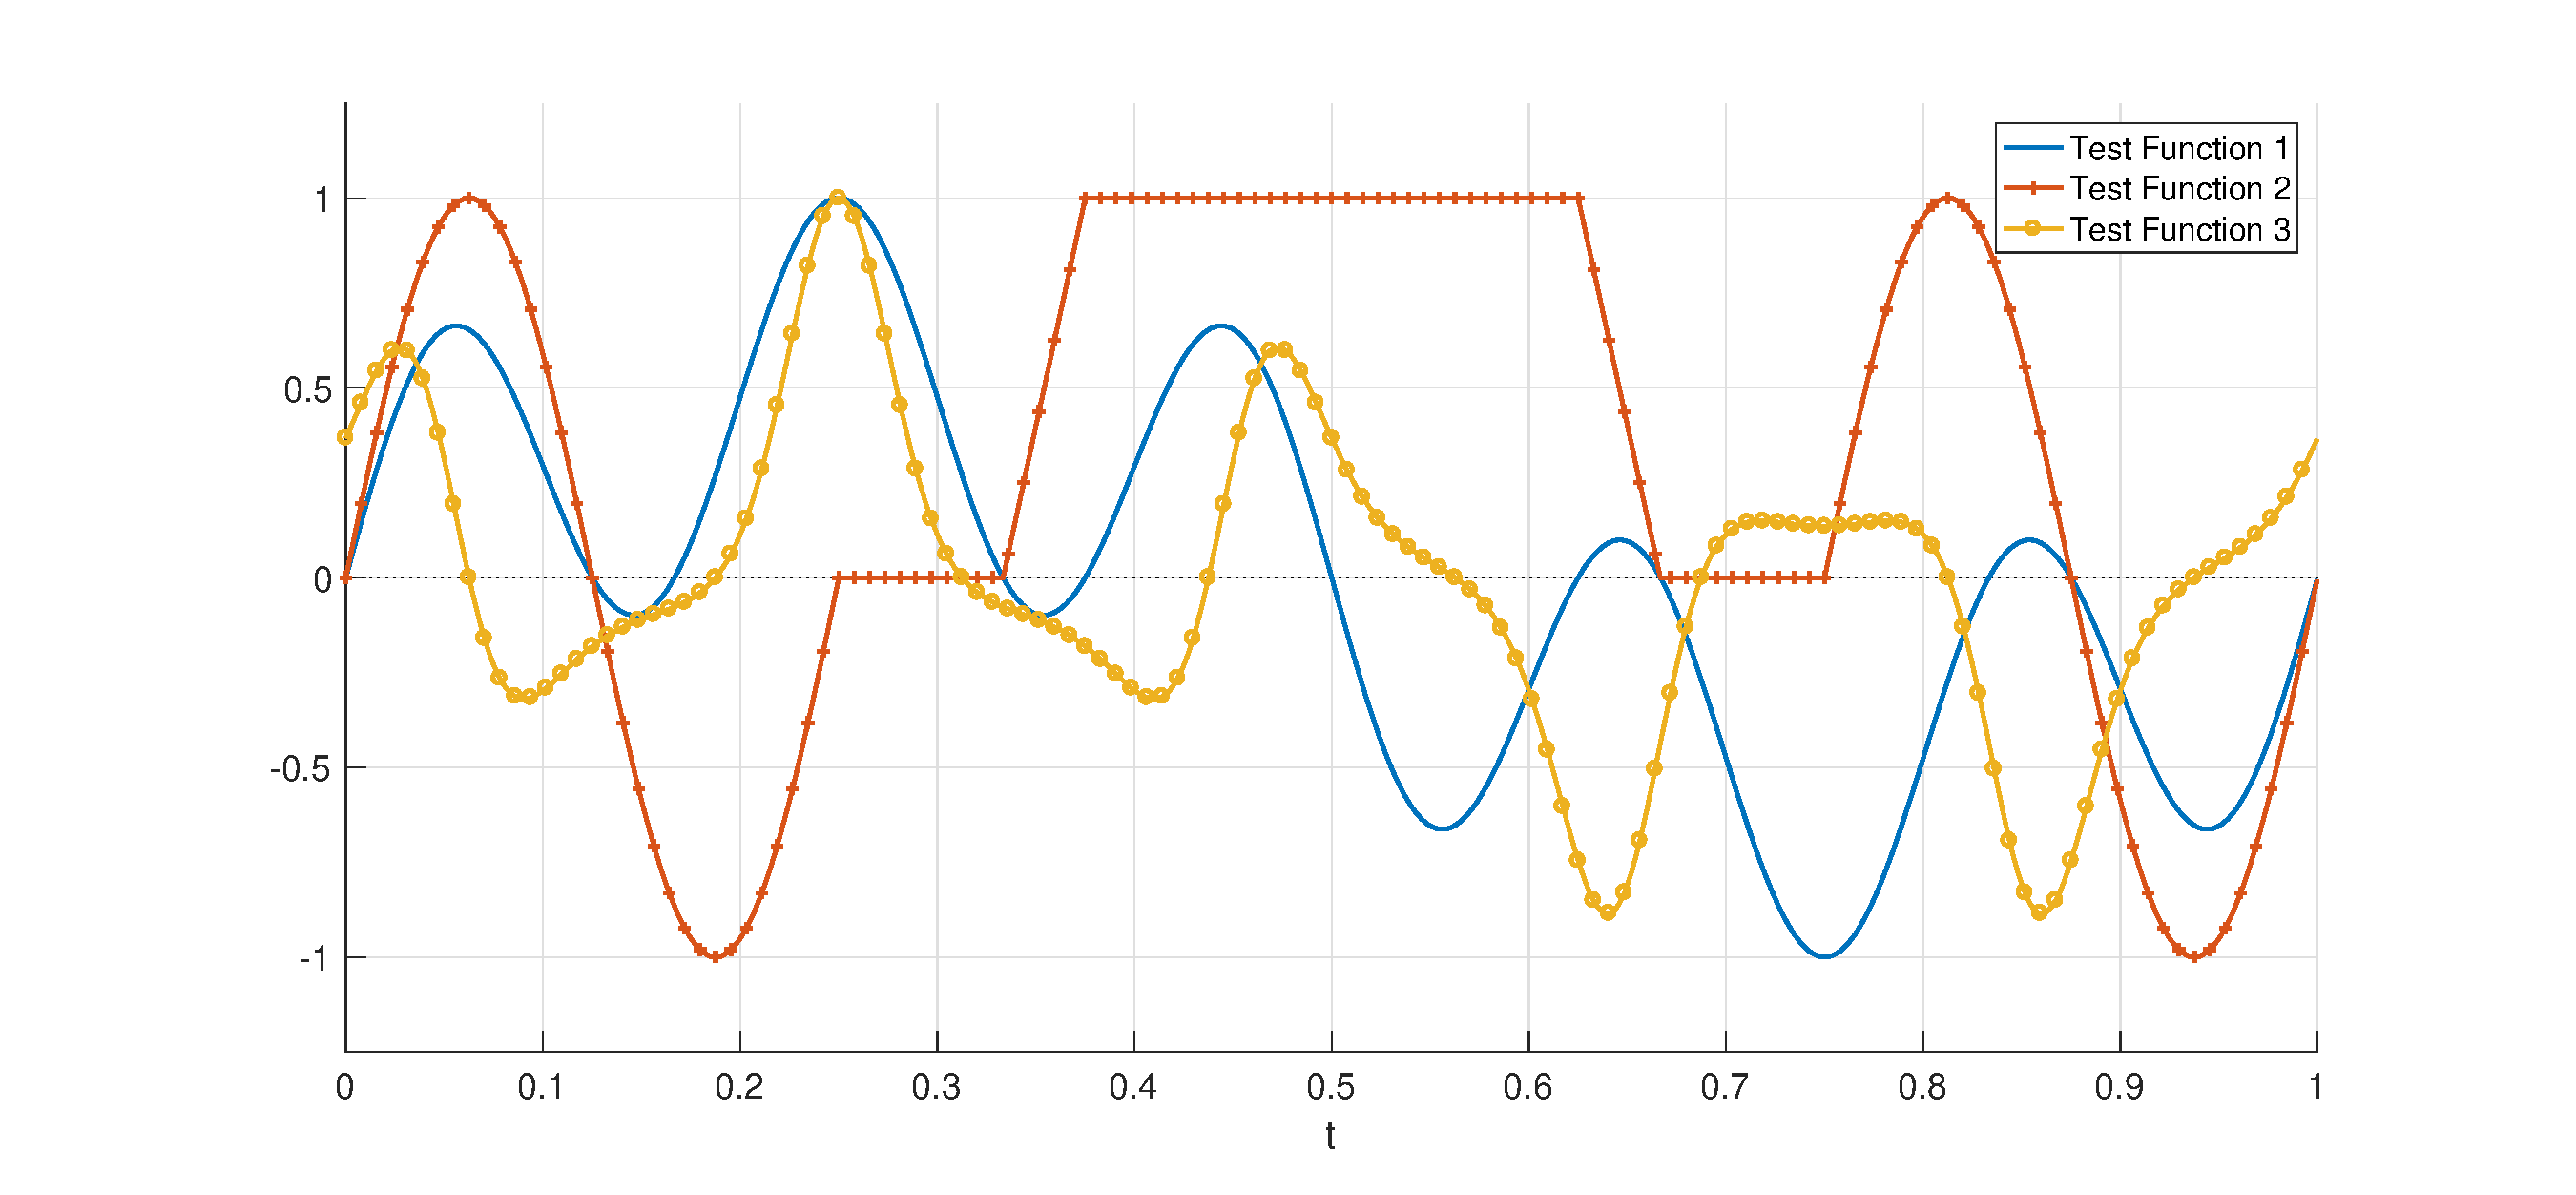
\includegraphics[scale = 0.45]{Figures/TestFunctions1D.eps}}
\caption{The three test functions considered in the numerical examples. Note that the second test function is only piecewise-smooth, while the first and second functions are smooth.}
\label{TestFunctions}
\end{figure}

The interval $[0,1]$ is discretized as equispaced points $0, 1/N, 2/N, \ldots, (N-1)/N$ for $N = 4096$. In other words, the interval is discretized as the vector $\tVec = [t_0,t_1,\ldots,t_{N-1}]$ with $t_\ell = \ell/N$. Samples of $g(x)$ are given at these points so that the discrete date $\gVec = [g_0,g_1,\ldots,g_{N-1}]$ has elements $g_\ell = g(t_\ell)$. The truncated Gaussian kernel $k(x,t)$ is assumed to be centered at the origin and compactly supported on the interval $[-\frac{1}{2},\frac{1}{2}]$. In the numerical examples, the width of the Gaussian kernels (i.e. the value of $1/2\noiseSD^2$ in \eqref{eq:Gaussian kernel}) is chosen to be 100 and 200. With a support of $[-\frac{1}{2},\frac{1}{2}]$, the test functions $f(t)$ must be defined on the interval $[-\frac{1}{2},\frac{3}{2}]$ for the convolution to be defined; see Chapter \ref{ch:Introduction}. As stated at the beginning of this chapter, $f(t)$ is initially defined over the interval $[0,1]$ and so the extensions of $f(t)$ on $[-\frac{1}{2},0)$ and $(1,\frac{3}{2}]$ will reflect the boundary condition being imposed.

%\begin{figure}
%	\centerline{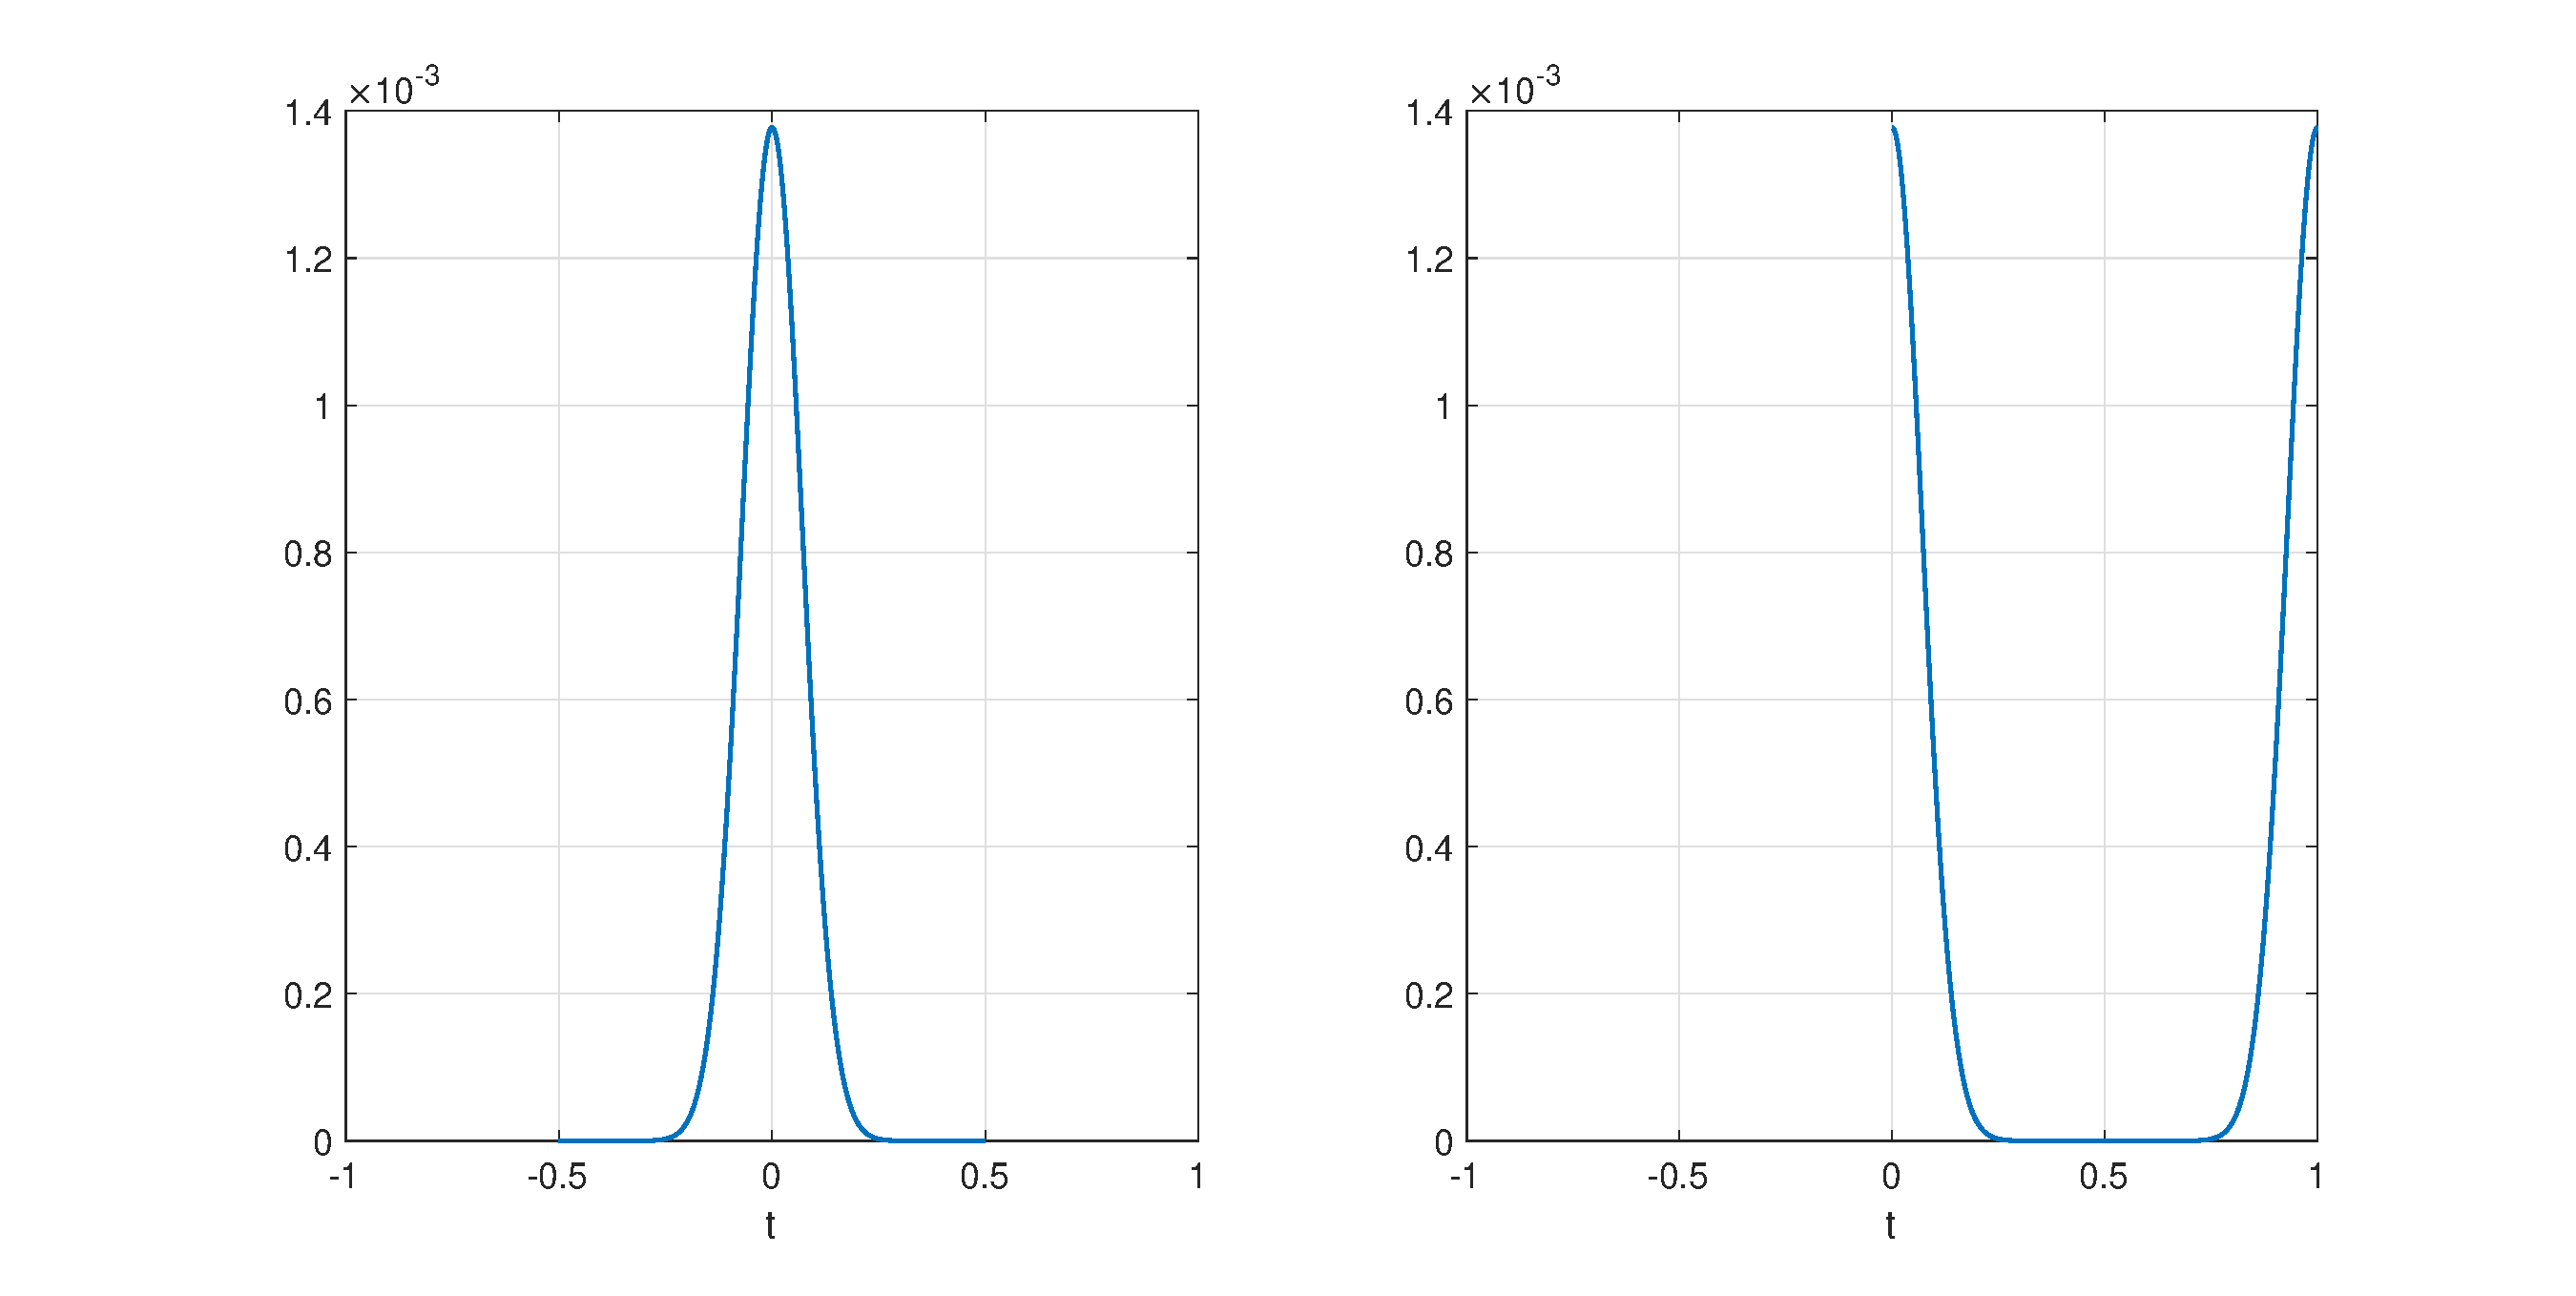
\includegraphics[scale = 0.45]{Figures/RegAndTroughGaussian.eps}}
%\caption{Plots of different discretizations of the kernel $k(t)$. The discretization on the left reflects the compact support of $k(t)$ on the interval $[-1/2,1/2]$. The discretization on the right represents the periodic extension of $k(t)$ on the interval $[0,1]$.}
%\label{RegAndTroughGaussian}
%\end{figure}

With the discretizations $\fVec$ and $\kVec$ determined, the discretization $\gVec$ of $g(t)$ can be evaluation using either a circular convolution or a linear convolution with appropriate vector padding. Ultimately the vectors $\fVec$, $\kVec$, and $\gVec$ are vector discretizations of $f(t)$, $k(x-t)$, and $g(t)$, respectively. \par
Overall, two selections for the width of the Gaussian kernel, two selections 5 and 25 for SNR value, and three test functions lead to a total of 12 configurations. For each configuration, 20 noise realizations were generated and tested. The full resolution problem was constructed using $N = 4096$ points. The downsamped resolutions were selected as $n \in \{16,32,\ldots,2048\}$ for a total of nine resolutions (eight values of $n$). \par 
A primary challenge of using the UPRE method with downsampled signals is that for a course downsampling (in other words, a small number of sample points), the resulting UPRE graphs are shallow. This shallowness makes finding a minimum difficult, and sometime the selected parameter is too small. Figure \ref{fig:UPRElambdas} shows that there are often outlier parameters that are too small, even sometimes for downsamplings with a moderate number of points. At $n = 16$, the range of the parameter values is larger than for the other downsampling levels, which can also be attributed to the shallowness of the function graphs. \par 
A consequence of choosing the regularization parameter to be too small is that the resulting relative errors are large; the outliers in Figure \ref{fig:UPREerrors} are the relative errors corresponding to the parameter outliers in Figure \ref{fig:UPRElambdas}. Unfortunately the error outliers can be significant, as even evidenced by the outlier at the full $N = 4096$ level. \par 
Fortunately, the averaged UPRE method appears to overcome the effects of the outliers. Figure \ref{fig:UPRElambdas} shows that for each downsampling level, the parameter found using the average UPRE method was larger than the mean of the parameters found by applying the UPRE to the noise realizations individually. As a result, the corresponding relative errors are less than the means of the errors for each downsampling level, displayed in Figure \ref{fig:UPREerrors}. However, the benefit derived from using the averaged UPRE method might be a consequence of the outliers themselves. Following the approximate region of the minimums of the UPRE functions (shown in Figure \ref{fig:UPREfunctions}), the functions increase rapidly. Thus functions that are excessively shallow may have this region of rapid increase located before the region of the minimums of the other functions. It could be the case that when the average UPRE function is formed, these outlier regions of rapid increase might push the final minimum toward a location that is actually beyond the region of the minimums of the non-outlier functions, resulting in a parameter that is larger than the mean of the individual parameters. Of course, this analysis is not rigorous and perhaps worthy of further investigation. 

% \begin{figure}
% 	\centering
% 	\begin{subfigure}[b]{0.45\textwidth}
%         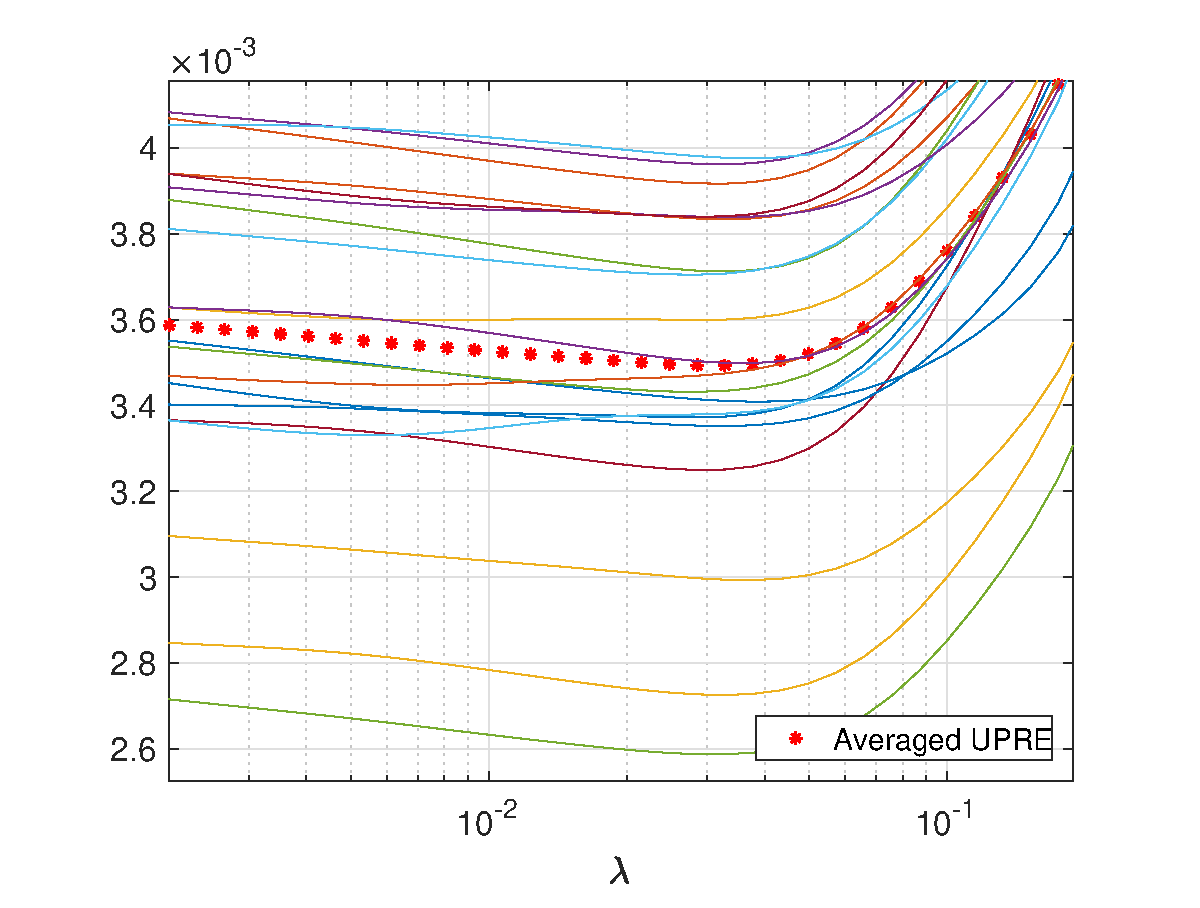
\includegraphics[width=\textwidth]{Figures/UPRE_AvgPlot1D_F1_S15_W100_R20.eps}
%         \caption{}
%         \label{fig:UPREfunctions}
%     \end{subfigure}
%     \begin{subfigure}[b]{0.45\textwidth}
%         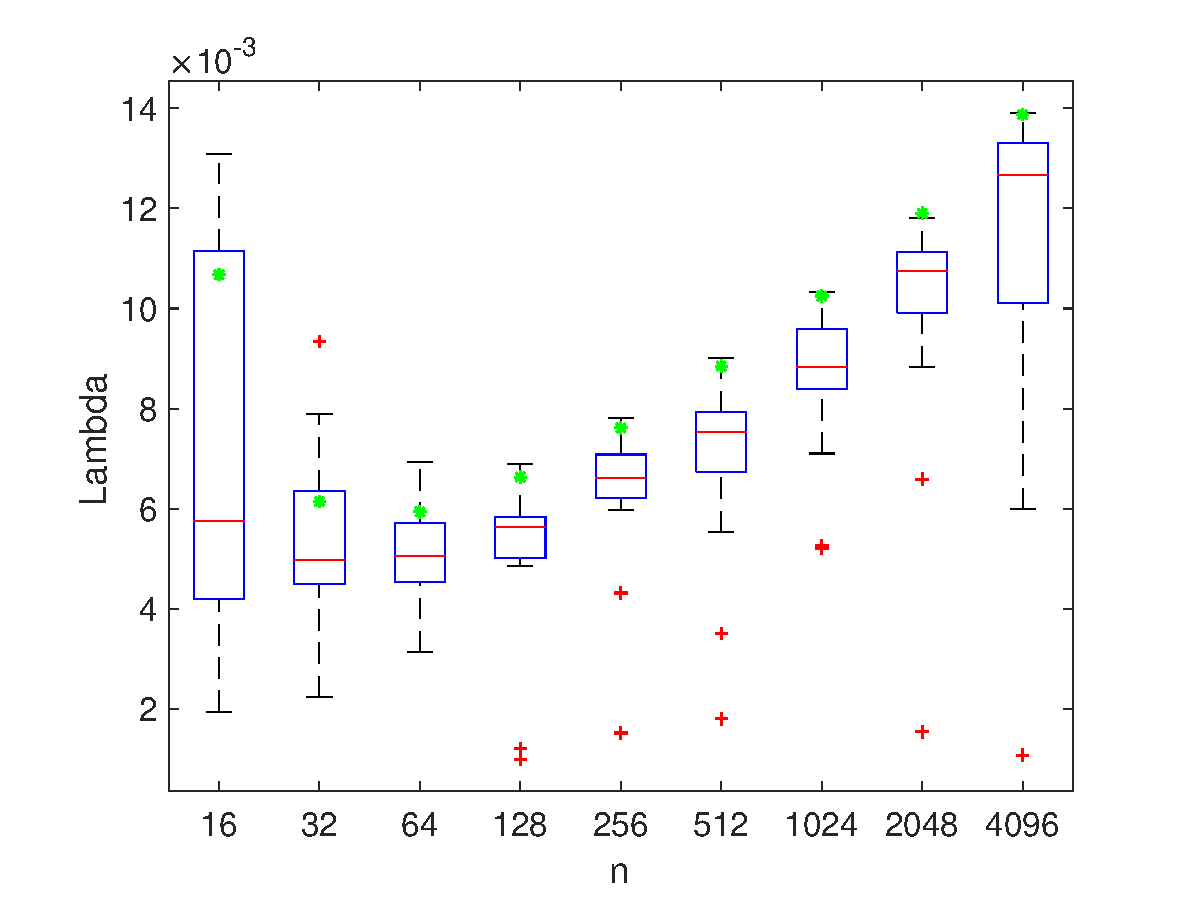
\includegraphics[width=\textwidth]{Figures/UPRE_LamPlot1D_F1_S15_W100_R20.eps}
%         \caption{}
%         \label{fig:UPRElambdas}
%     \end{subfigure}
%     \begin{subfigure}[b]{0.45\textwidth}
%         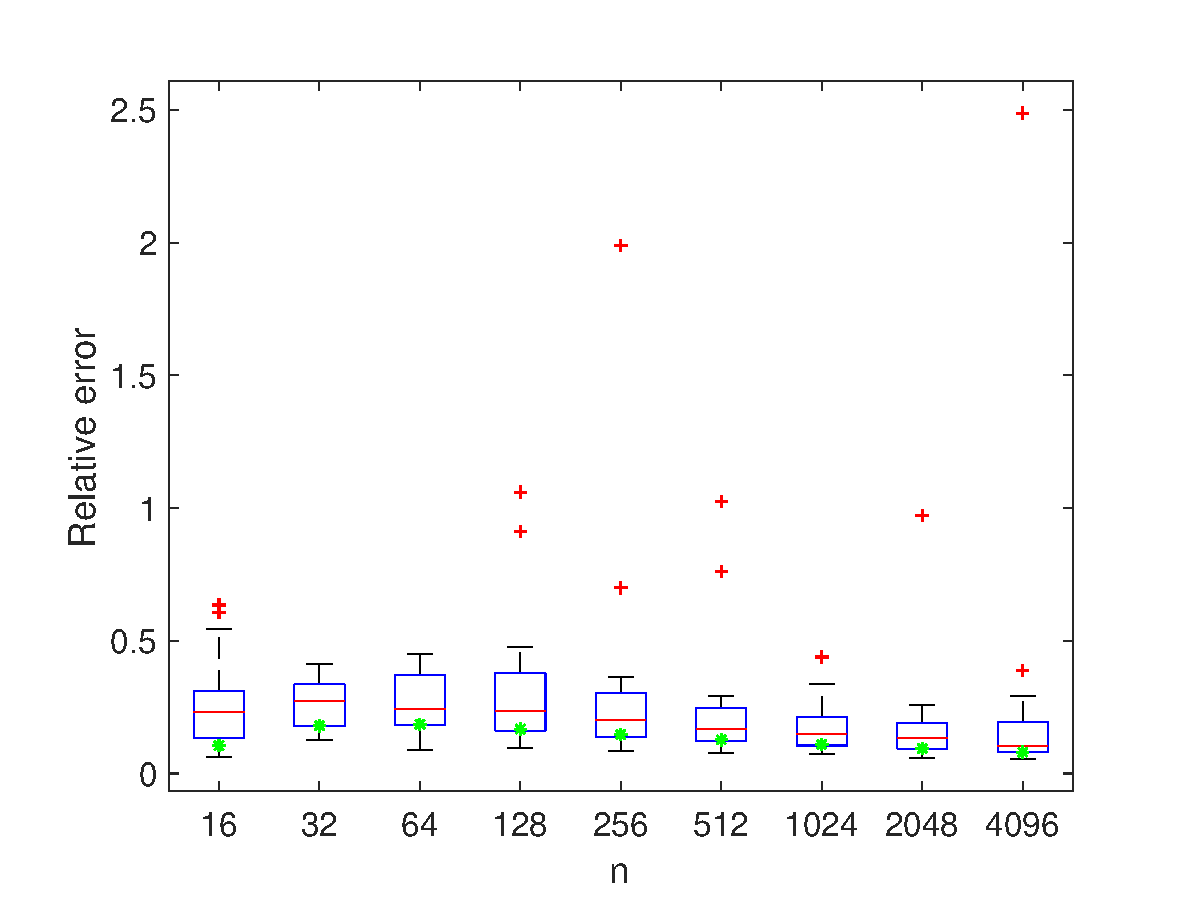
\includegraphics[width=\textwidth]{Figures/UPRE_ErrPlot1D_F1_S15_W100_R20.eps}
%         \caption{}
%         \label{fig:UPREerrors}
%     \end{subfigure}
%     \caption{Three plots showing the averaged UPRE results for the first test function with an SNR of 15 and  a Gaussian width parameter of 100. Figure \ref{fig:UPREfunctions} shows a zoomed-in portion of the averaged UPRE graph in comparison with graphs pertaining to the 20 noise realizations at a downsampling level of $n = 128$. Figure \ref{fig:UPRElambdas} shows that the resulting regularization parameter is typically greater than the average of the individual regularization parameters. Figure \ref{fig:UPREerrors} shows that the relative error corresponding to the parameter chosen from the average UPRE method is less than the average of the individual relative errors.}
% \label{fig:UPREplots}
% \end{figure} 

The numerical results of the GCV method are similar to those of the UPRE method. At times the graphs of the GCV functions are shallow and thus difficult to minimize. This is apparent from the parameter outliers in Figure \ref{fig:GCVlambdas} and the corresponding error outliers in Figure \ref{fig:GCVerrors}. The range of the parameters selected at the $n = 16$ is again significant. Some of the parameters at this level were selected so small (quite near to zero) so that the relative errors were excessively large; the largest relative error was approximately 35, and as a result the vertical axis in Figure \ref{fig:GCVerrors} had to be scaled so that errors larger than 2 are simply grouped in a non-scaled region to produce a tractable plot. \par 
In contrast to the UPRE method, the averaged version of the GCV method selected a regularization parameter that was worse than those selected by using individual noise realizations. The consequence of this is that the corresponding relative errors were larger than the mean of the individual relative errors. Thus the averaged GCV method does not appear to be a viable parameter selection approach.
%As previously mentioned, for the minimization-based methods UPRE and GCV, the shallowness of some of the curves made finding a meaningful minimum difficult. The approach that might be worth considering is to find the location of maximum curvature, which follows the observations and analysis presented in \cite{HansenOLeary}. \par 
%The signed curvature of a function $f$, assuming appropriate differentiablility, is
%\begin{equation}
%\kappa(x) = \frac{f''(x)}{(1+(f'(x))^2)^{3/2}}.
%\label{Eq:Curvature}
%\end{equation}
%Including the sign of the curvature is useful since a location of maximum curvature could be associated with local maximum instead of a minimum. A numerical approximation to \eqref{Eq:Curvature} can be readily obtained by discretizing $f$ on the domain of interest and using the finite difference approximations
%\[f'(x) \approx \frac{x_{j+1} - x_{j}}{\Delta{x}} \text{ and } f''(x) \approx \frac{x_{j-1} - 2x_j + x_{j+1}}{(\Delta{x})^2}\]
%for approximations of the derivatives. In MATLAB, the built-in function \texttt{diff} can be used to generate the derivative approximations. \par 
%Once a discretization of curvature is obtained, the location of maximum curvature is determined and this location is taken to be the regularization parameter from the UPRE and GCV methods. While the approach of maximizing curvature is not the same as finding a minimum a function itself, this approach could avoid the numerical challenges of minimizing the shallow UPRE and GCV functions. 

% \begin{figure}
% 	\centering
% 	\begin{subfigure}[b]{0.45\textwidth}
%         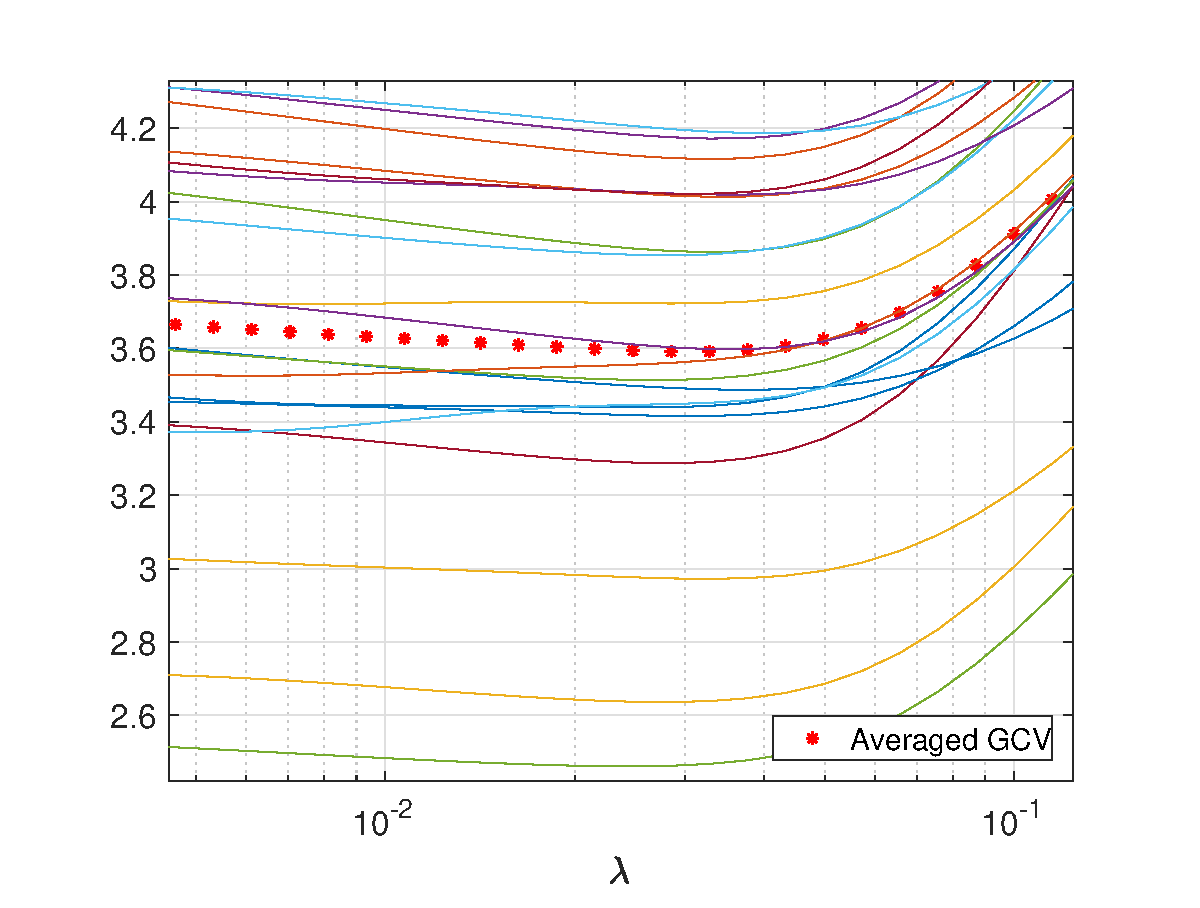
\includegraphics[width=\textwidth]{Figures/GCV_AvgPlot1D_F1_S15_W100_R20.eps}
%         \caption{}
%         \label{fig:GCVfunctions}
%     \end{subfigure}
%     \begin{subfigure}[b]{0.45\textwidth}
%         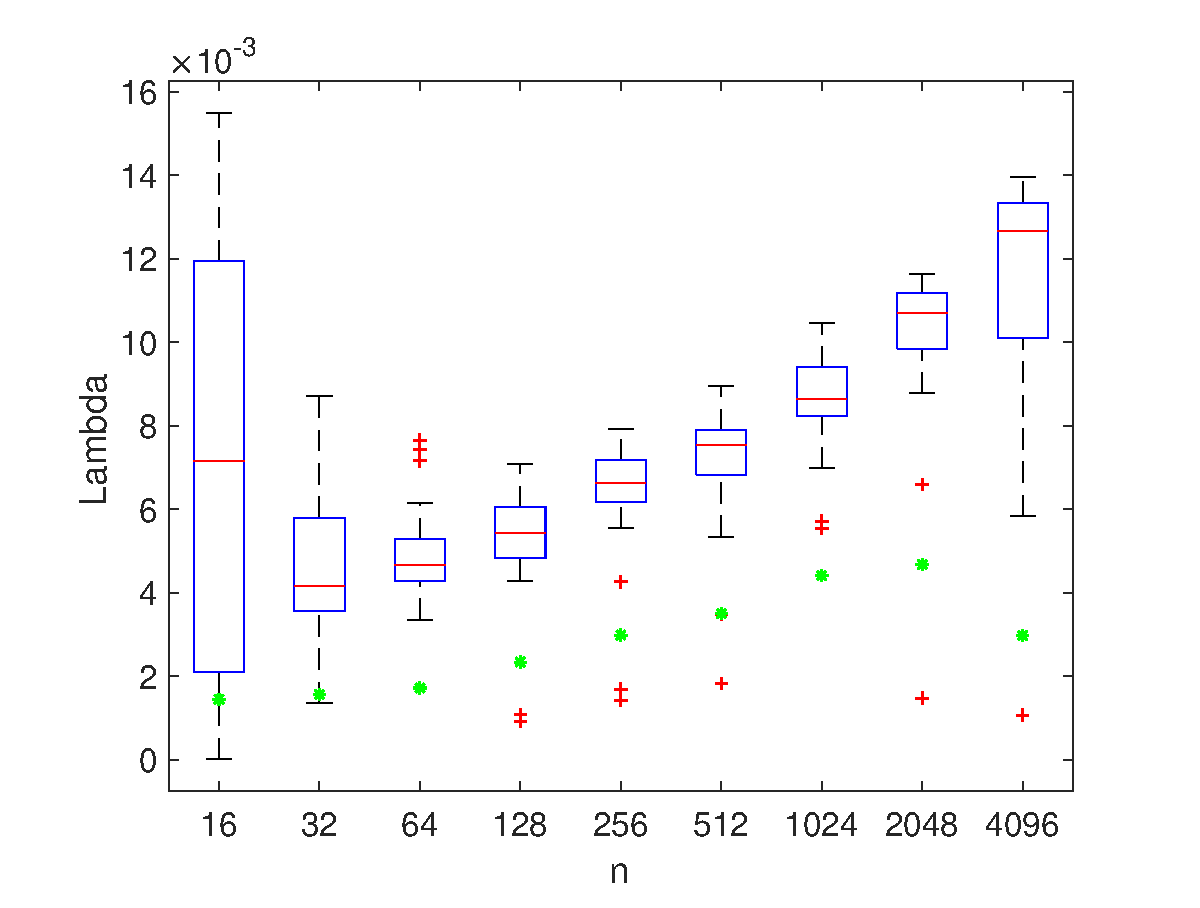
\includegraphics[width=\textwidth]{Figures/GCV_LamPlot1D_F1_S15_W100_R20.eps}
%         \caption{}
%         \label{fig:GCVlambdas}
%     \end{subfigure}
%     \begin{subfigure}[b]{0.45\textwidth}
%         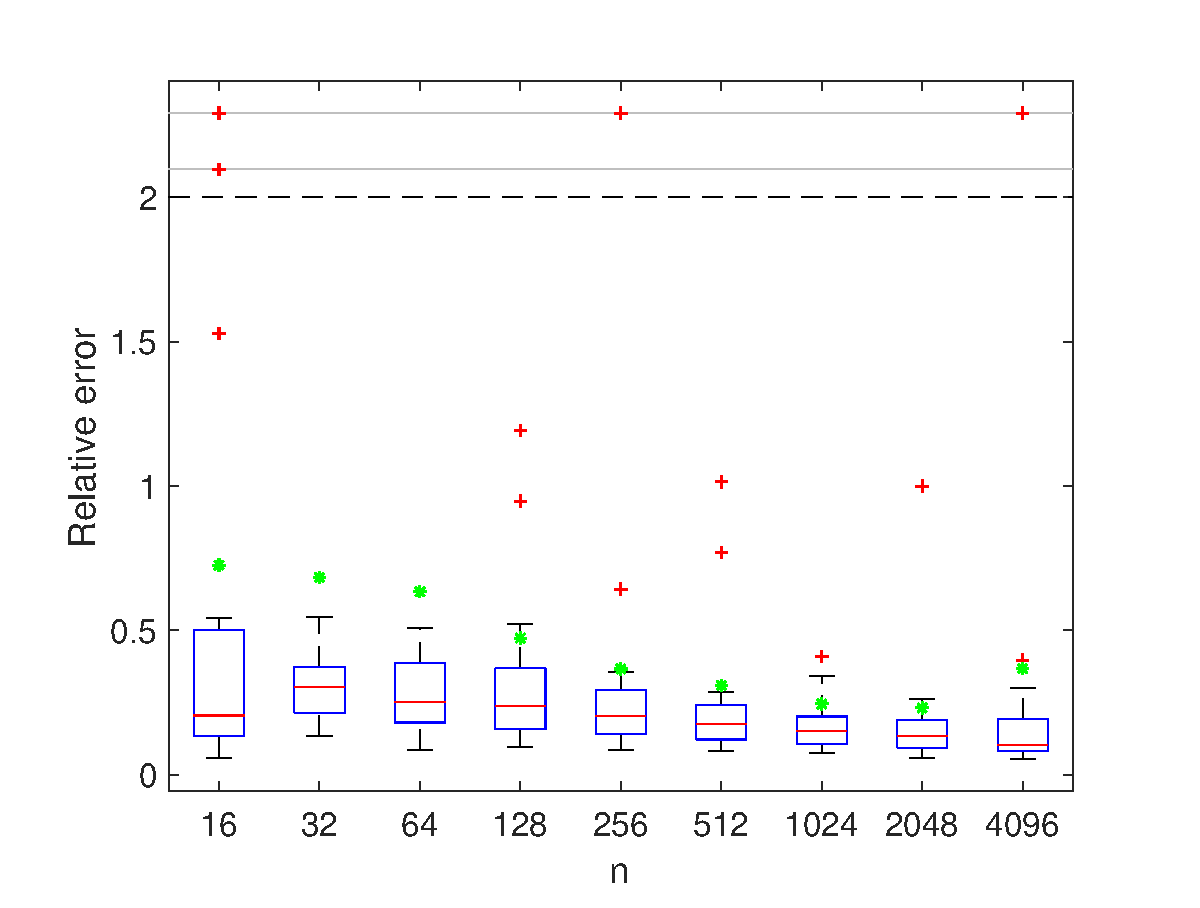
\includegraphics[width=\textwidth]{Figures/GCV_ErrPlot1D_F1_S15_W100_R20.eps}
%         \caption{}
%         \label{fig:GCVerrors}
%     \end{subfigure}
%     \caption{Three plots showing the averaged GCV results for the first test function with an SNR of 15 and a Gaussian width parameter of 100. Figure \ref{fig:GCVfunctions} shows a zoomed-in portion of the averaged GCV graph in comparison with graphs pertaining to the 20 noise realizations at a downsampling level of $n = 128$. Figure \ref{fig:GCVlambdas} shows that the resulting regularization parameter is typically less than the average of the individual regularization parameters. Figure \ref{fig:GCVerrors} shows that the relative error corresponding to the parameter chosen from the average GCV method is greater than the average of the individual relative errors.}
% \label{fig:GCVplots}
% \end{figure}

\chapter{The DCT approach} \label{ch:DCT}

The first boundary condition that will be considered is the Neumann boundary condition, defined by setting
\[\begin{cases}
f_{-1} = f_0 \\
f_{-2} = f_1 \\
\vdots \\
f_{-m+2} = f_{n-1}
\end{cases} ~ \text{and} ~
\begin{cases}
f_{n} = f_{n-1} \\
f_{n+1} = f_{n-2} \\
\vdots \\
f_{n+m-1} = f_{n-m}
\end{cases}.\]
Letting $J$ denote the $n \times n$ exchange matrix, the Neumann boundary condition allows for \eqref{eq: Tf = g} to be written as
\begin{equation}
\label{eq:Neumann Kf = g}
K\fVec = [(0~|~T_{l})J + T + (T_{r}~|~0)J]\fVec = \gVec,
\end{equation}
where $(0~|~T_{l})$ and $(T_{r}~|~0)$ are the $n \times n$ Toeplitz matrices formed by augmenting $T_{l}$ and $T_{r}$ with $n-m+1$ zero columns. As a result, the matrices $(0~|~T_{l})J$ and $(T_{r}~|~0)J$ are Hankel matrices. Therefore since $T$ is a Toeplitz matrix, the sum $[(0~|~T_{l})J + T + (T_{r}~|~0)J]$ is a Toeplitz-plus-Hankel matrix. Fortunately, this type of matrix is diagonalized by the DCT as stated in Section \ref{sec:Discrete trig. transforms}. The DCT-versions of the UPRE function \eqref{eq:UPRE DCT}, the GCV function \eqref{eq:GCV DCT}, and the discrepancy principle function \eqref{eq:DP DCT} can thus be used to select the Tikhonov regularization parameter $\regparam$. \par 
An version of the Downsampling Theorem can be obtained for the DCT. First, the following lemma will be established.
\begin{lemma}
Let $\mathbf{x} \in \mathbb{C}^N$, where $N = LM$ for positive integers $L$ and $M$. Then
\begin{align*}
\Re\left(\alias_L(\mathbf{x})\right) = \alias_L\left(\Re(\mathbf{x})\right), \\
\Im\left(\alias_L(\mathbf{x})\right) = \alias_L\left(\Im(\mathbf{x})\right).
\end{align*}
\end{lemma}
\begin{proof}
Let $\mathbf{a} = \Re(\alias_L(\mathbf{x}))$ and $\mathbf{b} = \alias_L(\Re(\mathbf{x}))$. By the definition of the aliasing operator and the linearity of taking the real part,
\[a_j = \Re\left(\sum_{k=0}^{L-1} x_{j+kM}\right) = \sum_{k=0}^{L-1} \Re(x_{j+kM}) = b_j.\]
The proof for the imaginary part is identical.
\end{proof}

A two-dimensional Fredholm integral equation of the first kind is
\begin{equation}
g(x,y) = \int_c^d \int_a^b k(x,y,s,t)f(s,t)~ds~dt.
\label{eq:FIE_2D}
\end{equation}
If the kernel satisfies $k(x,y,s,t) = k(x-s,y-t)$ and the limits of integration are infinite, then \eqref{eq:FIE_2D} represents two-dimensional convolution:
\begin{equation}
g(x,y) = \iint_{\mathbb{R}^2} k(x-s,y-t)f(s,t)~ds~dt.
\label{eq:Con_2D}
\end{equation}
Since an image can be considered a function $f : \mathbb{R}^2 \rightarrow \mathbb{R}$, the process of finding solutions to equations of the form \eqref{eq:Con_2D} is commonly referred to \textit{image deblurring}. For an extensive handling of image deblurring techniques, see \cite{HansenNagyOLeary} and \cite[Ch.~5]{Vogel:2002}. \par
If the support of $k(x-s,y-t)$ is $[a_k,b_k] \times [c_k,d_k]$ and information about $g(x,y)$ is known only in $[a_g,b_g] \times [c_g,d_g]$, then the integral equations for the values of $g(x,y)$ on the vertices of the rectangles are
\begin{align*}
g(a_g,c_g) &= \int_{c_g-d_k}^{c_g-c_k} \int_{a_g-b_k}^{a_g-a_k} k(a_g-s,c_g-t)f(s,t)~ds~dt \\
g(b_g,c_g) &= \int_{c_g-d_k}^{c_g-c_k} \int_{b_g-b_k}^{b_g-a_k} k(b_g-s,c_g-t)f(s,t)~ds~dt \\
g(b_g,d_g) &= \int_{d_g-d_k}^{d_g-c_k} \int_{b_g-b_k}^{b_g-a_k} k(b_g-s,d_g-t)f(s,t)~ds~dt \\
g(a_g,d_g) &= \int_{d_g-d_k}^{d_g-c_k} \int_{a_g-b_k}^{a_g-a_k} k(a_g-s,d_g-t)f(s,t)~ds~dt.
\end{align*}
For the sake of simplicity, assume that the support of $k(x-s,y-t)$ is $[-\frac{1}{2},\frac{1}{2}] \times [-\frac{1}{2},\frac{1}{2}]$ and information about $g(x,y)$ is known only in the unit square $[0,1] \times [0,1]$. Then
\begin{align*}
g(0,0) &= \int_{-\frac{1}{2}}^{\frac{1}{2}} \int_{-\frac{1}{2}}^{\frac{1}{2}} k(-s,-t)f(s,t)~ds~dt \\
g(1,0) &= \int_{-\frac{1}{2}}^{\frac{1}{2}} \int_{\frac{1}{2}}^{\frac{3}{2}} k(1-s,-t)f(s,t)~ds~dt \\
g(1,1) &= \int_{\frac{1}{2}}^{\frac{3}{2}} \int_{\frac{1}{2}}^{\frac{3}{2}} k(1-s,1-t)f(s,t)~ds~dt \\
g(0,1) &= \int_{\frac{1}{2}}^{\frac{3}{2}} \int_{-\frac{1}{2}}^{\frac{1}{2}} k(-s,1-t)f(s,t)~ds~dt.
\end{align*}
From these equations, the domain of definition of $f(s,t)$ needed for the existence of the integrals is $[-\frac{1}{2},\frac{3}{2}] \times [-\frac{1}{2},\frac{3}{2}]$. Thus if information about $f(s,t)$ is only required in $[0,1] \times [0,1]$, boundary conditions must be imposed.

%\section{Resolution Analysis} \label{ch:Resolution Analysis}
%Our goal is to determine the efficacy of downsampling for regularization parameter estimation, the effects of downsampling on the parameter estimation methods must be carefully examined. The parameter estimation methods are considered from the perspective of the DFT, and so downsampling must be viewed from the same perspective. \par 
%One of the most powerful results pertaining to sampling a signal for use in Fourier analysis is the Shannon-Whittaker Sampling Theorem, which is given here without proof. The version of the theorem pertains to the Fourier transform, defined for a function $f \in L^1(\mathbb{R})$ by
%\begin{equation}
%\dft{f}(\omega) = \frac{1}{\sqrt{2\pi}}\int_{-\infty}^{\infty} f(t)\exp(-i\omega{t})\: dt. 
%\label{eq:FourierTransform}
%\end{equation}
%The variable $\omega$ represents frequency. 
%\begin{SWST}
%Suppose that $\dft{f}(\omega)$ is continuous, piecewise smooth, and $\dft{f}(\omega) = 0$ for $|\omega| > \Omega$, where $\Omega$ is some fixed, positive frequency. Then $f = \mathcal{F}^{-1}(\dft{f})$ is completely determined by its values at the points $t_j = j\pi/\Omega$ for $j = 0,\pm 1,\pm 2,\ldots$. More precisely, $f$ has the series expansion
%\[f(t) = \sum_{j=-\infty}^{\infty} f\left(\frac{j\pi}{\Omega}\right)\frac{\sin(\Omega{t}-j\pi)}{\Omega{t}-j\pi},\]
%which converges uniformly. 
%\end{SWST}
%Given the smallest frequency $\Omega$ such that $\dft{f}(\omega) = 0$ for $|\omega| > \Omega$, the quantity $\Omega/2\pi$ is called the \textit{Nyquist frequency} and the quantity $\Omega/\pi$ is called the \textit{Nyquist rate}. Functions for which $\Omega$ exists such that $\dft{f}(\omega) = 0$ for $|\omega| > \Omega$ are called \textit{band-limited}. \par 
%The test function $f(x) = \cos(4\pi{t})\sin(6\pi{t})$ is band-limited. Applying a product-to-sum identity allows for the function to be rewritten as
%\begin{equation}
%f(t) = \cos(4\pi{t})\sin(6\pi{t}) = \frac{1}{2}\left[\sin(10\pi{t}) + \sin(2\pi{t})\right].
%\label{eq:Test Function 1}
%\end{equation}
%Though $f$ is not in $L^1(\mathbb{R})$, its Fourier transform can be express using the Dirac delta function:
%\begin{equation}
%\dft{f}(\omega) = i\frac{\sqrt{\pi}}{2\sqrt{2}}\left[\delta(\omega - 10\pi) +\delta(\omega - 2\pi) - \delta(\omega + 2\pi) - \delta(\omega + 10\pi)\right].
%\label{eq:Test Function 1 FT}
%\end{equation}
%It is now clear from \eqref{eq:Test Function 1 FT} that $f$ is indeed band-limited because $\dft{f}(\omega) = 0$ for $|\omega| > 10$. The Sampling Theorem then states that $f$ must be sampled at greater than 20 equispaced points per unit interval for exact reconstruction. If the number of sample points is selected as a power of 2 (which is advantageous for computation of DFT's), then sampling $f$ at $2^5 = 32$ points would be ideal; a smaller power, such as $2^4 = 16$, would be insufficient in that the reconstruction would suffer from the effects of aliasing. \par 
%In contrast, the second test function \eqref{eq:Test Function 2} is not band-limited. This can be seen by computing the Fourier transform of the piece of $f$ on $[3/8,5/8]$:
%\begin{equation} 
%\int_{3/8}^{5/8} \exp(-i\omega{t}) \: dt = \frac{2\exp(-i\omega/2)\sin(\omega/8)}{\omega}.
%\label{eq:Test Function 2 FT}
%\end{equation}
%Certainly there does not exist an $\Omega > 0$ such that the expression in \eqref{eq:Test Function 2 FT} is zero for all $|\omega| > \Omega$.

%Depending upon the structure of $A$ in \eqref{eq:Ax = b}, the process of constructing regularized solutions can be conducted in a frequency domain rather than a spatial domain. The frequency domain we consider in this paper is the one produced from the discrete Fourier transform (DFT). The DFT is a mapping $\mathcal{F}:\mathbb{C}^n \rightarrow \mathbb{C}^n$ defined by
%\begin{equation}
%\mathcal{F}(\mathbf{f})_j = \frac{1}{\sqrt{n}}\sum_{\ell=0}^{n-1} f_{\ell}\exp\left(\frac{-2\pi{ij\ell}}{n}\right), \quad \mathbf{f}\in\mathbb{C}^n, \quad 0 \leq k \leq n-1.
%\label{eq:DFT}
%\end{equation}
%The DFT of a vector $\mathbf{f}$ will be denoted by $\widehat{\mathbf{f}}$. The inverse DFT of a vector $\widehat{\mathbf{f}}$ is given by
%\begin{equation}
%\mathcal{F}^{-1}(\widehat{\mathbf{f}})_j = \frac{1}{\sqrt{n}}\sum_{\ell=0}^{n-1} \widehat{f}_\ell\exp\left(\frac{2\pi{ij\ell}}{n}\right) = f_j.
%\end{equation}
%These definitions are nonstandard; typically the factors $1/\sqrt{n}$ in both the forward and inverse DFT definitions are combined as a single factor of $1/n$ in the definition of the forward DFT. The DFT can also be stated in terms of matrix-vector multiplication. Given an $\mathbf{f} \in \mathbb{C}^n$, $\widehat{\mathbf{f}}$ can be expressed as $F\mathbf{f}$ where the matrix $F\in\mathbb{C}^{n\times{n}}$ has components
%\begin{equation}
%F_{j,k} = \frac{1}{\sqrt{n}}\exp\left(\frac{-2\pi{ijk}}{n}\right), \quad 0 \leq j,k \leq n-1.
%\label{eq:DFT-Matrix}
%\end{equation}
%The matrix representing the inverse DFT is then $\trans{F}$, where $\trans{}$ denotes conjugate transposition. A property of $F$ is that $\trans{F}F = F\trans{F} = (1/n)\diag(n) = I$, and so splitting the factor of $1/n$ as $(1/\sqrt{n})(1/\sqrt{n})$ for the definition of the DFT provides the benefit of $F$ being a unitary matrix. A direct consequence of the DFT being unitary is Parseval's theorem: $\|\mathbf{f}\| = \|F\mathbf{f}\|$ for any $\mathbf{f} \in \mathbb{C}^n$. Another useful property of $F$ is that if $C$ is a circulant matrix, then $C = \trans{F}\Delta{F}$ where $\Delta = \diag(\sqrt{n}\dft{\mathbf{c}})$ and $\mathbf{c}$ is the first column of $C$.

\chapter{Conclusions and future work} \label{ch:Conclusion}
Overall the numerical results demonstrate some potential viability of downsampling to obtain regularization parameters. At the least, the graphs in Sections \ref{sec:Numerical results (DFT)} and \ref{sec:Numerical results (DCT)} show that the statistics of the regularization parameters obtained have structure. The DFT and DCT versions of the UPRE, GCV, and discrepancy principle functions in Chapter \ref{ch:Parameter estimation methods} are useful when the two transforms are to be used in the inversion process. The corresponding statistical results of the function in Chapter \ref{ch:Parameter estimation methods}, such as \eqref{eq:UPRE Expected Value} and \eqref{eq:UPRE Var Sum Simple}, could be useful from an analytic standpoint. \par 
There are many possible directions of future work. The most important is to quantify the statistics of the regularization parameters when downsampling is applied. Fortunately the DFT and DCT are topics which have been thoroughly investigated in a number of settings. For example, there are explicit connections between downsampling and aliasing with regard to the DFT presented in \cite[Ch.~7]{AudioDFT}; versions of these results could be derived for DCT.  Another means of quantification could be to utilize the statistics of the parameter estimation functions and try to estimate intervals in which $\regparam$ will be found for each downsampling level. In some information about the frequency content (in regard to the DFT or DCT) of the continuous solution $f(t)$ is available, then the information can be used to select an appropriate downsampling level to capture the overall behavior of the solution; the ideal result would be to explicitly show how this process effects the resulting value of $\regparam$. \par 
Another direction of future work would be to investigate the situation where multiple data sets are available. The UPRE, GCV, and discrepancy principle functions for the availability of multiple data sets are \eqref{eq:SpectralUPREavg}, \eqref{eq:SpectralGCVsum}, and \eqref{eq:SpectralDPavg}, respectively. While the assumption of multiple data sets could produce some interesting results, this assumption is not appropriate for all applications. One issue is that repeated measurements cost time and additional resources. Another issue is that repeated measurements could alter the solution itself. For example, computed tomographic imaging used X-rays to obtain measurements regarding the internal structure of the object \cite[p.~12-14]{ABT} In the object in question is a human being, repeated measurements can result in cell damage. \par 
As a final and overarching direction for future work, three-dimensional problems will be considered. Examples of setting that produce three-dimensional inverse problems include computed tomography and subsurface imaging by gravitational measurements \cite{ABT}. The primary challenges of working with three-dimensional problems are the numerical structure of the problems themselves, such as how to correctly express the problems as matrix-vector product, as well as the computational costs of solving the problems. However, three-dimensional problems could be the types of problems where downsampling is most useful. To illustrate this intuition, if the unit cube $[0,1] \times [0,1] \times [0,1]$ is discretized by using the vector $[0,\frac{1}{4},\frac{1}{2},\frac{3}{4}]$ along each dimension, then downsampling to the vector $[0,\frac{1}{2}]$ reduces the number of points from 64 to 8. While the quantitative effects of downsampling should be determined before moving to three-dimensional problems, three-dimensional problems possess the most potential for demonstrating these effects.


%-----------------------back matter

{\singlespace
% Making the references a "part" rather than a chapter gets it indented at
% level -1 according to the chart: top of page 4 of the document at
% ftp://tug.ctan.org/pub/tex-archive/macros/latex/contrib/tocloft/tocloft.pdf
\addcontentsline{toc}{part}{REFERENCES}
\bibliographystyle{asudis}
\bibliography{Parameter-Estimation}}

\renewcommand{\chaptername}{APPENDIX}
\addtocontents{toc}{APPENDIX \par}
\appendix
\chapter{Derivation of multiparameter UPRE function}
\newpage
\label{sec:Multi UPRE Derivation}


%\include{appendices/appendix4}

\end{document}
%